\documentclass[12pt,twoside]{report} % Two-sided, reduce the size of the inner margins

% \usepackage{setspace}\doublespacing
\usepackage{setspace}\onehalfspacing

% \usepackage[nochapters]{classicthesis} % nochapters
\usepackage[sc]{mathpazo}

% Packages
% \usepackage[a4paper,top=30mm,bottom=30mm,inner=20mm,outer=20mm,bindingoffset=10mm,showframe=True]{geometry}
\usepackage[a4paper,top=30mm,bottom=30mm,inner=20mm,outer=20mm,bindingoffset=10mm]{geometry}

\usepackage[utf8]{inputenc}
\usepackage{graphicx}
\usepackage{geometry}
%\usepackage{mathtools}
\usepackage{listings}
\usepackage[table]{xcolor}
\usepackage{multirow}
\usepackage{array}
\usepackage{caption}
\usepackage{subcaption}
\usepackage{hyperref}
\usepackage{amsmath}
\usepackage{amssymb}
\usepackage{booktabs}
\usepackage{rotating}
\usepackage{adjustbox}
\usepackage{quoting} % For quotes in chapters

\usepackage{printlen} % For making plots look right

\usepackage[
backend=biber,
style=numeric-comp,
sorting=none,
maxnames=3,
minnames=1
]{biblatex}
\addbibresource{refs.bib}

\usepackage{arydshln}
\usepackage{makecell}
\usepackage{pdflscape} % Landscape pdfs
\usepackage{minted} % For code

% xspace intelligently adds a space
\usepackage{xspace}

% Define custom colors
\definecolor{pomlightpurp}{rgb}{0.38, 0.07, 0.38}
\definecolor{pomdarkpurp}{rgb}{0.24, 0.01, 0.24}
\definecolor{pomcyan}{rgb}{0, 0.63, 1}
\definecolor{pomtech}{rgb}{0.77, 0, 0.29}
\definecolor{lightgray}{gray}{0.9}
\definecolor{mediumgray}{gray}{0.5}

% %~~~% Section Titles %~~~%
\usepackage{titlesec}

% Customize the style for numbered sections
\titleformat{\section}
  {\Large\bfseries\rmfamily} % Font style
  {\thesection}  % No prefix to section title
  {1em} % No spacing between prefix and title
  {} % Section numbering with space

\titleformat{\subsection}
  {\Large\bfseries\rmfamily} % Font style
  {}  % No prefix to section title
  {0em} % No spacing between prefix and title
  {\thesubsection\quad} % Section numbering with space
%~~~% %~~~% %~~~%


% %~~~% Chapter Titles %~~~%
% Define the custom chapter format
\titleformat{\chapter}[display] % Display style for chapter title
  {\Huge\bfseries\rmfamily} % Font style for chapter title
  {\filleft\fontsize{100}{110}\selectfont\color{pomlightpurp}{\thechapter}} % Large chapter number in purple
  {20pt} % Space between chapter number and title
  {\titlerule\vspace{1ex}\filleft} % Horizontal rule and vertical space, title aligned left
  [\vspace{1ex}\titlerule] % Horizontal rule after the title

% Adjust spacing before and after chapter title
\titlespacing*{\chapter}{0pt}{*5}{*5} % Adjust spacing before and after chapter title

% Define the custom numberless chapter format
\titleformat{name=\chapter,numberless}[display] % Display style for numberless chapter title
  {\Huge\bfseries\rmfamily\color{black}} % Font style for chapter title
  {} % No chapter number
  {0pt} % No space between number and title
  {\filleft} % Horizontal rule and vertical space, title aligned left

% Adjust spacing before and after numberless chapter title
\titlespacing*{\chapter}{0pt}{*3}{*4} % Adjust spacing before and after chapter title
%~~~% %~~~% %~~~%



% %~~~% Chapter Quotes %~~~%
% Define the custom quote formatting
\newcommand{\chapterquote}[1]{
  \begin{quote}
    \color{mediumgray}\itshape #1
  \end{quote}
}
%~~~% %~~~% %~~~%




%~~~% Text commands %~~~%
\newcommand{\gw}{gravitational wave\xspace}
\newcommand{\gws}{gravitational waves\xspace}
\newcommand{\Gw}{Gravitational wave\xspace}
\newcommand{\Gws}{Gravitational waves\xspace}
\newcommand{\scl}{scattered-light\xspace}
\newcommand{\Scl}{Scattered-light\xspace}
\newcommand{\cbc}{compact binary coalescence\xspace}
\newcommand{\cbcs}{compact binary coalescences\xspace}
\newcommand{\aligo}{Advanced LIGO\xspace}
%~~~% %~~~% %~~~%




%~~~% Header and Footer design %~~~%
\usepackage{fancyhdr}
\usepackage{pdfpages}
\usepackage{etoolbox}
\setlength{\headheight}{26pt}
\pagestyle{fancy}

% Define a command to include a specific PDF based on page number
\newcommand{\customsymbol}[1]{%
  \raisebox{-0.025\height}{%
    \includegraphics[width=1.5cm]{images/header/#1.pdf}
  }%
}

% Define a custom header for Arabic numerals pages
\newcommand{\arabicheader}{%
  \renewcommand{\headrule}{%
    \vspace{0pt}
    \hrulefill
    \raisebox{-10.0pt}{%
      \hspace{0.5em}%
      \customsymbol{\thepage} % Use the page number for the PDF file
    }%
    \hrulefill
  }
  \fancyhf{}
  \fancyhead[LE, RO]{\textbf{\thepage}}
  \fancyhead[CO]{\nouppercase{\leftmark}}
  \fancyhead[CE]{\nouppercase{\rightmark}}
  \fancyfoot{}
}

% Define a custom header for Roman numerals pages
\newcommand{\romanheader}{
    \fancyhf{}
    \renewcommand{\footrulewidth}{0.0pt}
    \renewcommand{\headrulewidth}{0.4pt}
    \fancyhead[LO, RE]{\textbf{\thepage}}
    \fancyhead[CO]{\nouppercase{\leftmark}}
    \fancyhead[CE]{\nouppercase{\rightmark}}
    \fancyfoot{}
    }

% Redefine \chaptermark to remove "Chapter X." 
% Redefine \sectionmark to remove the "X.X"
\renewcommand{\chaptermark}[1]{\markboth{#1}{}}
\renewcommand{\sectionmark}[1]{\markright{#1}}
%~~~% %~~~% %~~~%





%~~~% %~~~% %~~~% %~~~% %~~~% %~~~% %~~~% %~~~% %~~~%
%~~~% %~~~% %~~~% MAIN DOCUMENT %~~~% %~~~% %~~~%

%---%---%---%---%
\begin{document}

% Preliminary sections: title, abstract, etc.
\pagenumbering{roman} % Roman numerals for preliminary pages
\romanheader

%---% Title %---%
\begin{titlepage}
   \begin{center}

        \vspace*{1.5cm}

   
        \rule{\textwidth}{0.4pt}\\
        \vspace{0.4cm}
        \Huge \textbf{Improving the Detection of Gravitational-Wave Signals in Real Time}
        \rule{\textwidth}{0.4pt}

        \vspace{1.0cm}
        \textbf{Arthur Tolley}

        \vspace{1.0cm}
            
        {\large THE THESIS IS SUBMITTED IN PARTIAL FULFILMENT OF THE REQUIREMENTS FOR THE AWARD OF THE DEGREE OF DOCTOR OF PHILOSOPHY}\\
        {\large OF THE}\\
        {\large UNIVERSITY OF PORTSMOUTH}

        \vspace{2.0cm}
     
       
\includegraphics[width=0.6\textwidth]{images/preamble/UoP_Logo.pdf}
            
        \large October 2024
            
   \end{center}
\end{titlepage}

%---% Quote Page %---%
\chapter*{}
\null\vfill
% Now comes the "Funny Quote", written in italics
\textit{``Yesterday is history, tomorrow is a mystery, and today is a gift… that’s why they call it present''}

\begin{flushright}
Master Oogway
\end{flushright}

\vfill\vfill\vfill\vfill\vfill\vfill\null
\clearpage

%---% Declaration %---%
\chapter*{Declaration of Authorship}
Whilst registered as a candidate for the above degree, I have not been registered for any other research award. The results and conclusions embodied in this thesis are the work of the named candidate and have not been submitted for any other academic award.

\vspace{\baselineskip}
\noindent Ethical review code: ETHICS-10374

\vspace{\baselineskip}
\noindent Word count: 34,049

\noindent\hrulefill

\vspace{\baselineskip}
\noindent \textbf{Arthur Tolley}

\noindent \textbf{18th September 2024}

%---% Abstract %---%
\chapter*{Abstract}
\addcontentsline{toc}{chapter}{Abstract}
Lorem ipsum dolor...

%---% Dedication %---%
\chapter*{Dedication}
\addcontentsline{toc}{chapter}{Dedication}
I dedicate this document to myself.

\vspace{\baselineskip}

This document stands as proof of my perseverance, resilience and fortitude in completing one of the hardest journeys of my life, so far. For the countless hours of effort I am rewarded with this journey coming to an end, both with a reminiscence of the previous four years and an eagerness to visit the next lifetime of opportunities.

In moments of challenge and doubt, I found the strength to continue, to push the boundaries of my capabilities. In moments of success and accomplishment, I channeled the satisfaction and propelled myself toward new beginnings.

As I present this thesis, I take pride in the knowledge that my hard work, determination, and self-motivation have been woven into every page. This dedication serves as a reminder that self-belief and tenacity are the driving forces behind my academic journey.

I am proud of the knowledge I have gained, the skills I have honed, and the growth I have experienced. This dedication symbolizes self-recognition and a tribute to the part of me I invested in the pursuit of academic achievement.

\vspace{\baselineskip}

\textbf{Arthur Tolley}


%---% Acknowledgements %---%
\chapter*{Acknowledgements}
\addcontentsline{toc}{chapter}{Acknowledgements}
Enough of the big-headedness, there are over a hundred people who have each individually made me the person I am today and without them, their help, conversations, emotional support and even conflict, I would not be here at the end of this (very) long journey.

People: Ian, Andy, Mum, Dad, Lee, Jo, Claire, Vickie, Chris, Akash, Nick, Alex, Jake, Billy, George, Ricky, Muntazim, Connor W, Raf, Dan, Joe, Gareth, Ronaldas, Hooshyar, Christina, Toyah

%---% Table of Contents %---%
\tableofcontents

%---% List of Figures %---%
\listoffigures

%---% List of Tables %---%
\listoftables

% Reset page numbering and switch to Arabic numerals for main content
\cleardoublepage
\pagenumbering{arabic}
\arabicheader

%---% Introduction %---%
\chapter*{\label{chapter:introduction}Introduction}
\addcontentsline{toc}{chapter}{Introduction}
% General Relativity and Gravitational Waves
In the 20th century, Albert Einstein introduced the theory of \GR~\cite{Einstein_1:1914, Einstein_2:1914, Einstein_3:1914, Einstein_4:1915, Einstein_5:1916, Einstein_6:1917, Einstein_7:1936}, which describes gravity as the curvature of spacetime caused by massive objects, rather than as a force. In this framework, objects move along geodesics in curved spacetime. A key prediction of the theory is the existence of \gws~\cite{Einstein_8:1937, Einstein_9:1938, Einstein_10:1939, Einstein_11:1948}, which are perturbations in spacetime generated by the acceleration and collisions of massive bodies, such as black holes or neutron stars. These waves propagate at the speed of light and induce small changes in the proper distance between freely falling objects. The detector strain caused by \gws is extremely small, typically on the order of $10^{-22}$ for the most energetic sources, making direct detection highly challenging. Despite this, the observation of \gws has become a crucial tool for studying astrophysical phenomena and testing the predictions of \GR.

% First Direct Detection
The first direct detection of \gws occurred in 2015 with the observation of GW150914~\cite{GW150914:2016}, a \gwadj signal produced by the merger of two black holes. This event was detected by the Laser Interferometer Gravitational-Wave Observatory (LIGO) and the Virgo~\cite{aVirgo:2015} \gwadj observatory using ground-based interferometers. The observed signal matched the predictions of \GR~\cite{GW150914_TGR:2016} for the inspiral, merger, and ringdown phases of a binary black hole coalescence. This detection marked the beginning of \gwadj astronomy, providing the first direct evidence of black hole mergers and opening a new observational window to study the Universe.

% Expansion of Observations
Following the first detection of \gws, the global \gwadj detector network expanded with the inclusion of the KAGRA detector~\cite{KAGRA:2021}. The current International Gravitational-Wave Observatory Network (IGWN) collaboration has enabled more comprehensive and sensitive observations of \gwadj events. With a running total of 221 \gwadj events~\cite{gwtc1:2019, gwtc2:2021, gwtc21:2024, gwtc3:2023, 1OGC:2018, 2OGC:2020, 3OGC:2021, 4OGC:2021, Princeton_1:2019, Princeton_2:2019, Princeton_3a:2022, Princeton_3b:2023, gracedb_superevents:2024} from \cbcs, including two mergers of binary neutron star systems~\cite{GW170817:2017, GW190425:2020} and two neutron star–binary black hole mergers~\cite{nsbh:2021}, across four observing runs as of the drafting of this thesis.

% Thesis Scope
The work performed in this thesis focuses on improvements to the current search methods for \gws from data obtained by ground-based \gwadj observatories. Chapter~\ref{chapter:1-gravitational-waves} provides a simple derivation of \gws, a brief discussion of how the current generation of detectors operates, and the expected \gwadj emissions from a compact binary coalescence. This discussion is intended to give the reader a basic understanding of the background required to appreciate the motivation for the research conducted in later chapters; for texts with more detailed discussions, please refer to~\cite{Moore_book:2012, Maggiore_book:2007, Schutz_book:2009}. Chapter~\ref{chapter:2-searches} reviews the detection methods used for \gws, focusing on the PyCBC~\cite{PyCBC:2016} search pipeline. Chapter~\ref{chapter:3-detchar} concentrates on Detector Characterisation and the techniques employed to characterise and calibrate ground-based interferometer noise, producing high-quality data for further study.

Chapter~\ref{chapter:4-archenemy} investigates the feasibility of modelling \gwadj detector data artefacts, specifically the \scladj artefact, and subtracting these artefacts to clean the data before the search for \gws. In Chapter~\ref{chapter:5-pycbc-live}, we describe the improvements to the PyCBC Live search's ranking statistic aimed at enhancing detection sensitivity. Chapter~\ref{chapter:6-earlywarning} details the PyCBC Live Early Warning search, examining its deficiencies and suggesting improvements to ensure the identification of all potentially electromagnetically bright events. In Chapter~\ref{chapter:7-snr-optimiser}, we discuss the investigation and enhancements made to the PyCBC Live rapid detection statistic optimiser. Finally, in Chapter~\ref{chapter:8-industry}, we briefly discuss the industrial placements undertaken as a requirement of this doctoral programme.


%---% General Relativity %---%
\chapter[Gravitational Waves]{\label{chapter:1-gravitational-waves}Gravitational Waves}
\chapterquote{``The curvature of spacetime is a manifestation of gravity.'' - ChatGPT}
\section{\label{sec:GWs}Gravitational Waves}

This section will reproduce the derivation of \gws, closely following the textbook `A General Relativity Workbook' by Thomas A. Moore \cite{moore_2013}.

General Relativity (GR) is our current theory of gravitation in the Universe. GR introduces the Einstein field equations (EFEs), described by equation \ref{eqn:EFE}, which relate the curvature of spacetime to the matter and energy
within it. Solving EFEs is extremely difficult to do analytically so we must resort to looking at heavily simplified problems or using numerical relativity and the power of supercomputers.

\begin{equation}
   G^{\mu \nu} = 8 \pi G T^{\mu \nu}
   \label{eqn:EFE}
\end{equation}

Where $G^{\mu \nu}$ is the Einstein tensor, $G$ is Newton's constant of gravitation and, $T^{\mu \nu}$ is the stress-energy tensor.

One of the predictions of GR is the existence of \gws. To derive \gws with the Einstein field equations, we must begin with some assumptions about our spacetime. Far from the source of \gws, where the stress-energy tensor
$T^{\mu \nu} = 0$, we can describe the spacetime as flat with a tiny perturbation caused by the presence of \gws. Our metric can be described as follows:

\begin{equation}
   g_{\mu \nu} = \eta_{\mu \nu} + h_{\mu \nu}
   \label{eqn:g_mu_nu}
\end{equation}

Where $\eta_{\mu \nu}$ is the spacetime metric of flat spacetime and $h_{\mu \nu}$ is a small perturbation.

By saying that $h_{\mu \nu}$ is small ($|h_{\mu \nu}| << 1$) we can disregard all 2nd order and higher terms of $h_{\mu \nu}$, this is known as taking the weak-field limit. Using the metric $g_{\mu \nu}$ from equation \ref{eqn:g_mu_nu} with a linearized perturbation is known as linearized gravity.

We will proceed to work with the Einstein equation in the form:

\begin{equation}
   G^{\mu \nu} \equiv R^{\mu \nu} - \frac{1}{2} g^{\mu \nu} R = 8 \pi G T^{\mu \nu}
   \label{eqn:EFE2}
\end{equation}

Where $R^{\mu \nu}$ is the Ricci tensor and $R$ is the curvature scalar.

By substituting the trace-reversed metric perturbation:

\begin{equation}
   H^{\mu \nu} \equiv h^{\mu \nu} - \frac{1}{2} \eta^{\mu \nu} h
   \label{eqn:bigH}
\end{equation}

We get a form of the Einstein equation:

\begin{equation}
   \Box H^{\gamma \sigma} - \partial^\gamma \partial_\mu H^{\mu \sigma} - \partial^\sigma \partial_\mu H^{\mu \gamma}
   + \eta^{\gamma \sigma} \partial_\beta \partial_\mu H^{\mu \beta} = -16 \pi G T^{\gamma \sigma}
   \label{eqn:EE_long}
\end{equation}

Imposing the Lorentz gauge condition:

\begin{equation}
   \partial_\mu H^{\mu \nu} = 0
   \label{eqn:Lorentz_condition}
\end{equation}

Reduces equation \ref{eqn:EE_long} to:

\begin{equation}
   \Box H^{\mu \nu} = -16 \pi G T^{\mu \nu}
   \label{eqn:simple_EE}
\end{equation}

Where $\Box$ is the d'Alembertian operator, $\Box \equiv -\frac{\partial ^2}{\partial t^2} + \nabla^2$.

Reiterating our condition of weak-field, we can set the stress-energy tensor to 0:

\begin{equation}
   \Box H^{\mu \nu} = 0
   \label{eqn:wave_solutions}
\end{equation}

The solutions to equation \ref{eqn:wave_solutions} are plane waves
$H^{\mu \nu} = A^{\mu \nu} e^{i k_\alpha x^{\alpha}}$. $A_{\mu \nu}$ is the amplitude tensor, and, $k_\alpha = [-\omega, k_x, k_y, k_z]$ is the wave vector. Where $\omega$ is the angular frequency of the wave. The perturbations to flat spacetime appear as waves propagating through the universe, these are what we call `\gws'.

To further constrain our solutions to the simplest possible for, we consider a transformation to the gauge:

\begin{equation}
   x'^{\alpha} \equiv x^{\alpha} + \xi^{\alpha}
   \label{eqn:gauge_transformation}
\end{equation}

This is a very small transformation ($\xi^{\alpha} << 1$) and has no effect on $h_{\mu \nu}$ or $H_{\mu \nu}$ ($h_{\mu \nu} = h'_{\mu \nu}$ and $H_{\mu \nu} = H'_{\mu \nu}$). Therefore, we can impose another condition on our equations:

\begin{equation}
   \Box \xi^{\mu} = 0
   \label{eqn:gauge_trans_condition}
\end{equation}

Then if we take a gauge transformation of the form:

\begin{equation}
   \xi^{\mu} = B^{\mu} e^{i k_\alpha x^{\alpha}}
   \label{eqn:gauge_transformation_form}
\end{equation}

Which satisfies our condition in equation \ref{eqn:gauge_trans_condition}, we can take our amplitude tensor, $A_{\mu \nu}$, and transform it to a new $A_{\mu \nu}$ where:

\begin{equation}
    A^{t \mu} = A^{\mu t} = 0 \quad \text{and} \quad A^\mu_\mu = 0
    \label{eqn:TT_conditions}
\end{equation}

The first condition is telling us that all t-components of our tensor $A^{\mu \nu}$ are equal to 0 and the second condition states the trace of our tensor is also 0. This is known as the transverse-traceless (TT) gauge. The TT gauge enforces $h_{\mu \nu} = H_{\mu \nu}$, our amplitude tensor has a trace of 0 so our perturbation has no trace to reverse.

The final simplification we make is to consider the wave to be travelling exclusively in the $z$-direction. This gives a wave-vector $k_\sigma = [-\omega, 0, 0, \omega]$. Using the Lorentz gauge condition again (equation \ref{eqn:Lorentz_condition} where $H^{\mu \nu} = A^{\mu \nu} e^{i k_\alpha x^{\alpha}}$) we can see that $k_\mu A^{\mu \nu} = 0 = -\omega A^{t \nu} + \omega A^{z \nu}$ so $A^{t \nu} = A^{z \nu}$. We also know $A^{\mu \nu}$
is a symmetric tensor ($A^{\mu \nu} = A^{\nu \mu}$) and so $A^{z \nu} = A^{\nu z} = 0$.

These conditions and symmetries say that all $t$ and $z$ components of our amplitude tensor are 0. Further, the TT gauge is both traceless and symmetric so we can make assumptions about the remaining four terms. The TT gauge allows
only two polarizations of the waves: $A_{+}$, the plus polarization and; $A_{\times}$, the cross polarization.

\begin{equation}
   A_{\mu \nu} =
   \begin{pmatrix}
      0 & 0 & 0 & 0 \\
      0 & A_+ & A_\times & 0 \\
      0 & A_\times & -A_+ & 0 \\
      0 & 0 & 0 & 0
   \end{pmatrix}
   \label{eqn:A_mu_nu}
\end{equation}

\section{\label{sec:Mechanics}The Physical Effects of Gravitational Waves}

In order to detect \gws we must know how the presence of \gws changes some physical property that we can measure. We express our perturbation in the form $h_{\mu \nu}^{TT} = A_{\mu \nu} \cos(k_\sigma x^\sigma)$ (where superscript TT
indicates we are in the TT gauge and we have taken the real part of our plane wave solution) and consider a set of particles position in a ring of radius $R$, illustrated in figure \ref{fig:polarization}.

\begin{figure}
   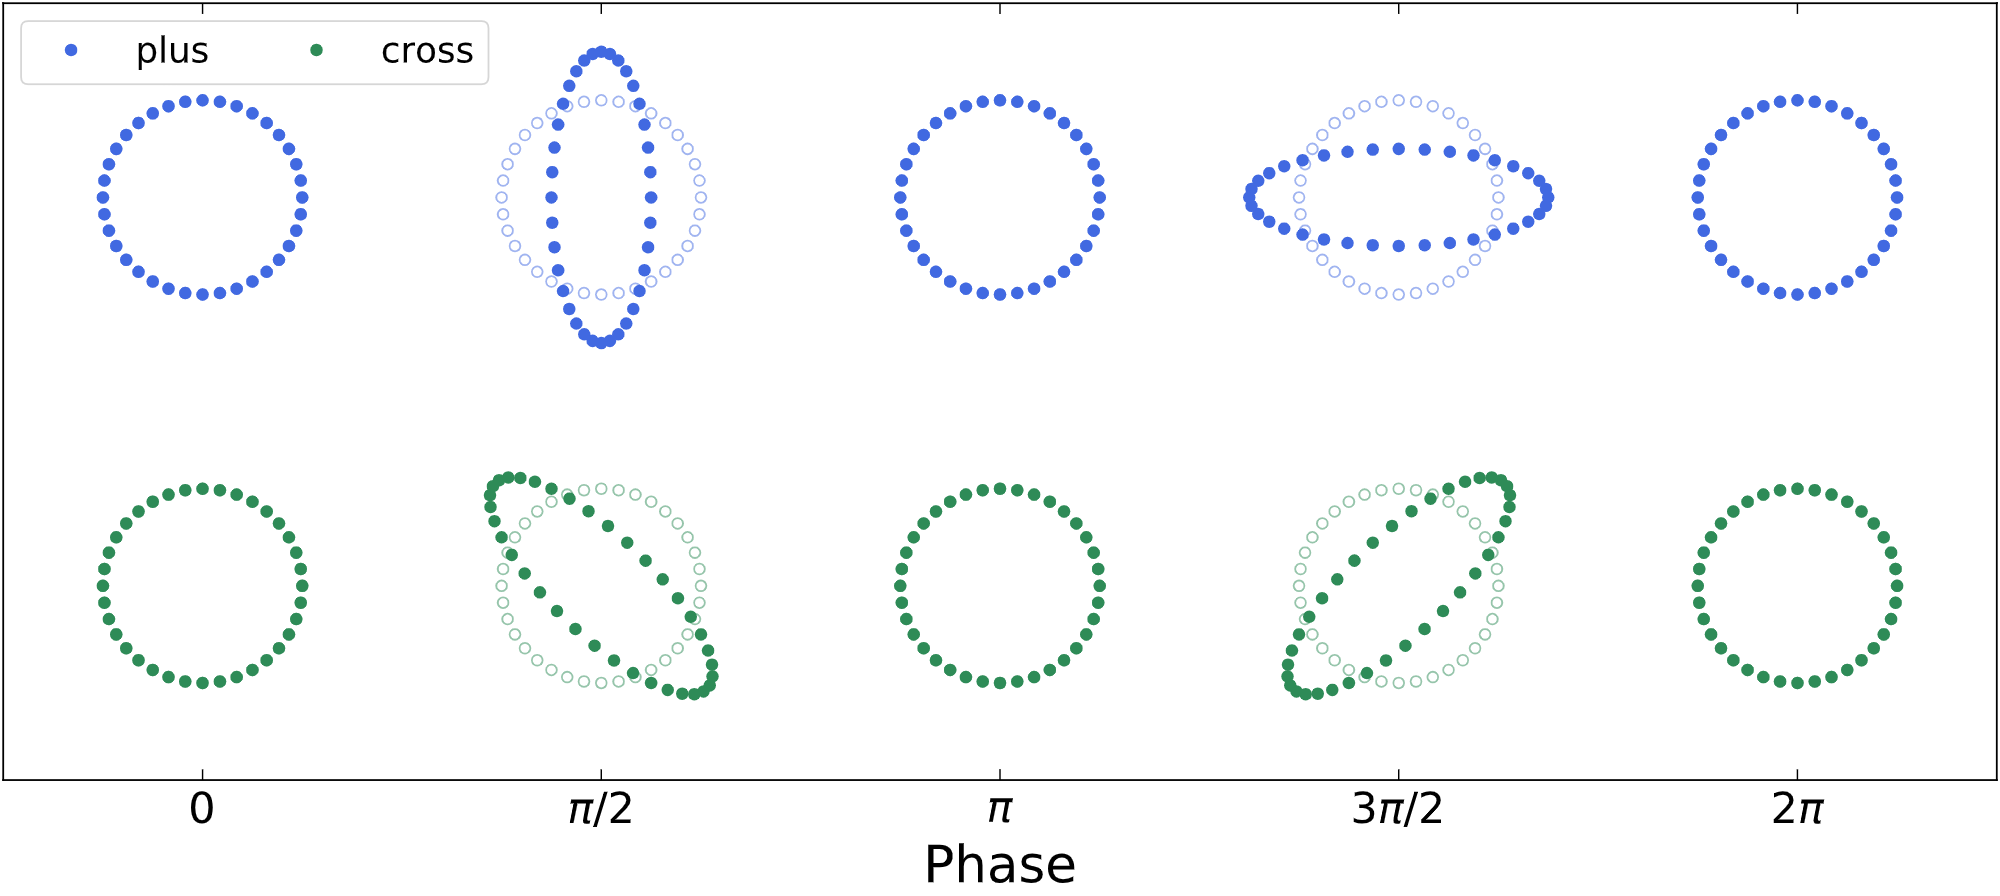
\includegraphics[width=\textwidth]{images/1_general_relativity/polarization.png}
   \caption{\label{fig:polarization}The effect of the two polarizations on a ring of test particles~\cite{gw_polarization_plots}.}
\end{figure}

A \gw polarized completely in the `plus' plane will produce a physical separation of any particle from the centre of the ring of:

\begin{equation}
   \Delta s = R[1 + \frac{1}{2} A_+ \cos(\omega t) \cos(2 \theta)]
   \label{eqn:plus_separation}
\end{equation}

Where $\Delta s$ is the physical separation of the particle from the centre, $R$ is the radius of the circle and, $\theta$ is the polar angle of each particle.

Likewise for a \gw completely polarized in the `cross' plane:

\begin{equation}
   \Delta s = R[1 + \frac{1}{2} A_{\times} \cos(\omega t) \sin(2 \theta)]
   \label{eqn:cross_separation}
\end{equation}

It is important to note that we are treating the separation between the particles and the centre in cartesian coordinates as the TT gauge is a comoving coordinate system where the coordinates of the particles are fixed
even as a \gw passes through.

\section{\label{sec:CBC}Gravitational Wave Sources - Compact Binary Coalescence}

A \cbc occurs when two stellar remnants, such as neutron stars (NSs) or black holes (BHs), in a binary system merge. This section will discuss \cbcs (CBCs) as a source of \gws.

The fraction of stars in binary systems is dependent on mass, research suggests that among very massive stars 80\% might be multiple-star systems \cite{binary_fraction:2006}. This is important as we look for black-hole binary (BBH) systems as one of the CBC sources of \gws. It is also worth mentioning that while most binary systems will form that way, there is the potential for a dynamic capture to occur where compact objects are flung and caught from
their system to other systems; especially in highly dense stellar neighbourhoods such as the centre of galaxies \cite{dynamic_capture:2000}.

Objects emit \gws continuously throughout their lifetimes, causing the orbit of the objects to lose energy and decay. Over the course of billions of years the radius decays until the two objects merge. The \gw frequency is twice that of the orbital frequency \cite{kip_book} and we can determine the frequency sweep (the change in the frequency over time) using the equation (discarding higher order terms for simplicity):

\begin{equation}
   \frac{dF}{dt} = \frac{96}{5 \pi \mathcal{M}^2} (\pi \mathcal{M} F)^{\frac{11}{3}}
   \label{eqn:frequency_sweep}
\end{equation}

Where $F$ is the \gw frequency and $\mathcal{M}$ is the chirp mass: total mass, $M = m_1 + m_2$; reduced mass, $\mu = m_1 m_2/(m_1+m_2)$, symmetric mass ratio $\eta = \mu/M$ then $\mathcal{M} = \eta^\frac{3}{5} M$ \cite{PE:1995}.

Equation \ref{eqn:frequency_sweep} shows that frequency of the \gw changes as a function of both the frequency and the chirp mass of the system. To higher order terms, the frequency evolution depends further on other parameters such as the spin-orbit and spin-spin parameter \cite{CBC_spin:1993}.

For a BBH in a circular orbit, the evolution of the system will depend on 8 parameters: the two masses and six spin components. Further complexities such as neutron stars (non-rigid bodies) or eccentric orbits will require more parameters.

\section{\label{sec:IFOs}Gravitational Wave Detection}

The detection of \gws is made possible by \gw observatories: LIGO consists of Hanford \& Livingston \cite{aLIGO:2015}; Virgo in Pisa \cite{aVirgo:2015}; KAGRA in Japan \cite{KAGRA:2021}; and GEO in Germany \cite{GEO600:2002}. This section will focus on
the design of the LIGO interferometers however, the techniques are similar for all detectors. The configuration of \aligo (aLIGO) is described in detail in the 2016 paper \cite{aLIGO:2015}.

\subsection{\label{sec:laser_interferometry}Laser Interferometry}

As seen in section \ref{sec:Mechanics}, the effects of \gws in cartesian coordinates is a stretching and squeezing of the ring of test particles. We can measure this using laser interferometry allowing the detection of the small
perturbations caused by the presence of \gws in spacetime.

We begin with a basic L-shaped Michelson interferometer, seen in figure \ref{fig:basic_michelson}:

\begin{figure}
   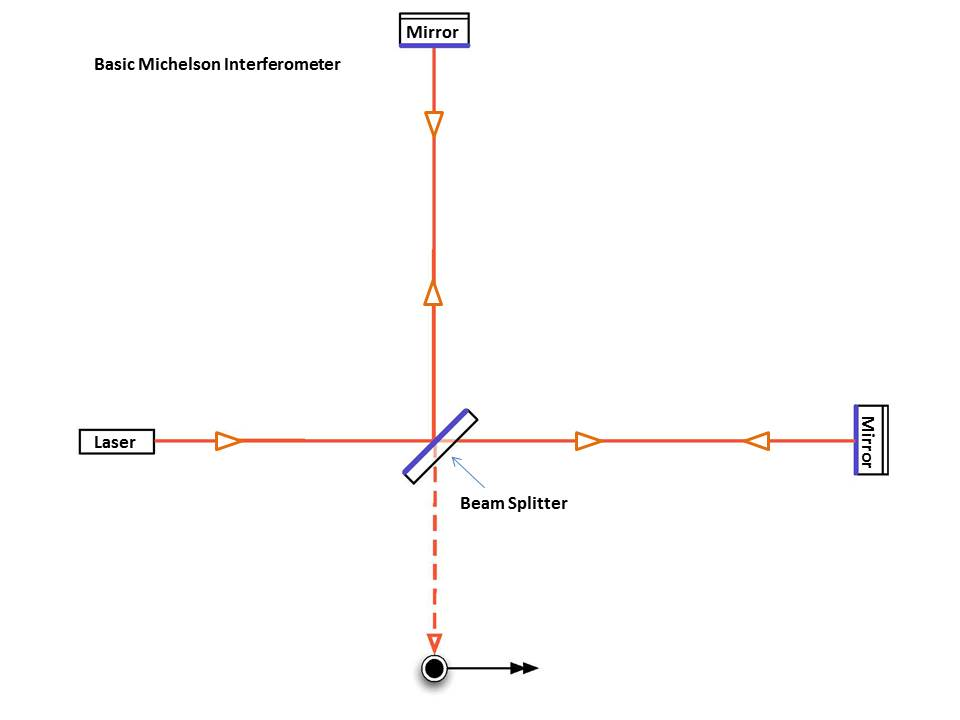
\includegraphics[width=\textwidth]{images/1_general_relativity/Basic_michelson_labeled.jpg}
   \caption{\label{fig:basic_michelson}A basic Michelson interferometer \cite{ligo_ifo}: A laser beam is shone at a beam splitter, the components are sent down equal length perpendicular arms where they reflect off the mirrors at the end, the components are then recombined back at the beam splitter and passed through to the photodetector (black circle) where the interference pattern of the laser is observed.}
\end{figure}

The LIGO detectors are identical in design with arm lengths of 4km, longer arms are able to make more precise measurements, looking at equations \ref{eqn:plus_separation} \& \ref{eqn:cross_separation}, the separation
$\Delta s$ depends on the radius $R$ (analogous to our arm length). We can further increase the distance our laser beam travels by using Fabry-Perot cavities to constantly recycle the laser in the arms. Figure \ref{fig:FP_michelson} shows the inclusion of Fabry-Perot cavities onto our basic Michelson interferometer.

\begin{figure}
   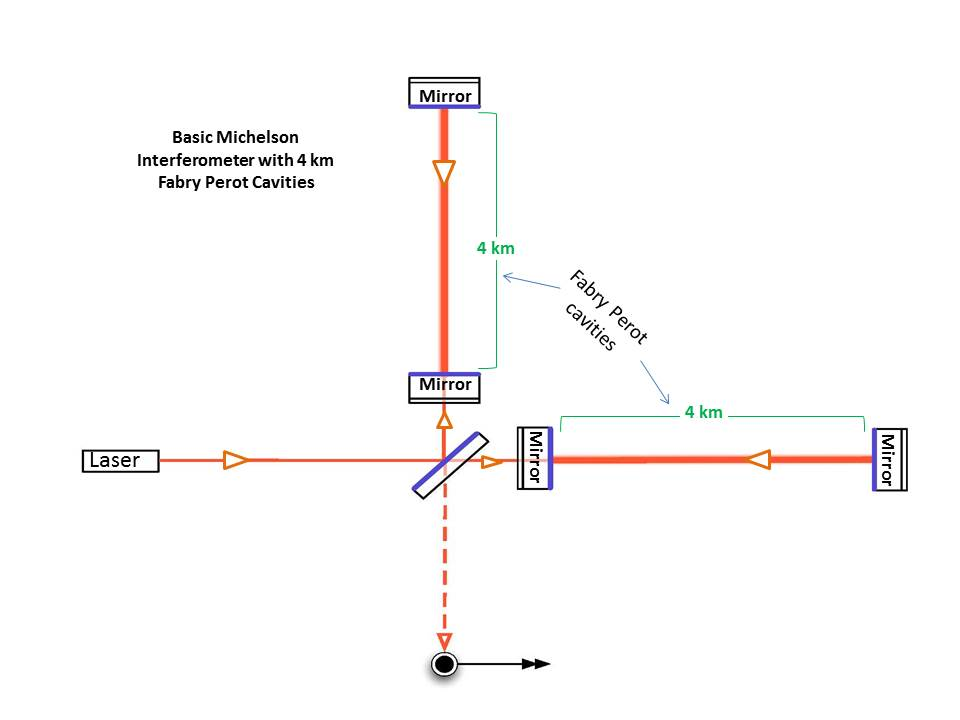
\includegraphics[width=\textwidth]{images/1_general_relativity/Basic_michelson_with_FP_labeled.jpg}
   \caption{\label{fig:FP_michelson}Fabry-Perot cavities \cite{ligo_ifo}: Additional mirrors are placed close to the beam splitter in each arm to allow the laser to traverse the arms many more times, effectively adding distance to our arms.}
\end{figure}

To create Fabry-Perot cavities extra mirrors are placed in each arm close to the beam splitter, these mirrors allow the laser to bounce back and forth within the arm many more times - effectively increasing the distance the laser has travelled. The Fabry-Perot cavities are fully evacuated, further reducing noise from the effects of interactions with particles in the air.

Laser power is continuously built up during this process, the more photons we have in our detector, the greater the resolution at our photodetector. We need to reach a laser power much higher than at the source, the Fabry-Perot
cavities don't provide enough amplification so we need to implement power recycling mirrors prior to the laser reaching the beam splitter. Some of the light from the laser is reflected towards the photodetector from the beam
splitter, the rest of it is sent back to the power recycling mirror. The power recycling mirrors can be seen in figure \ref{fig:IFO}.

\begin{figure}
   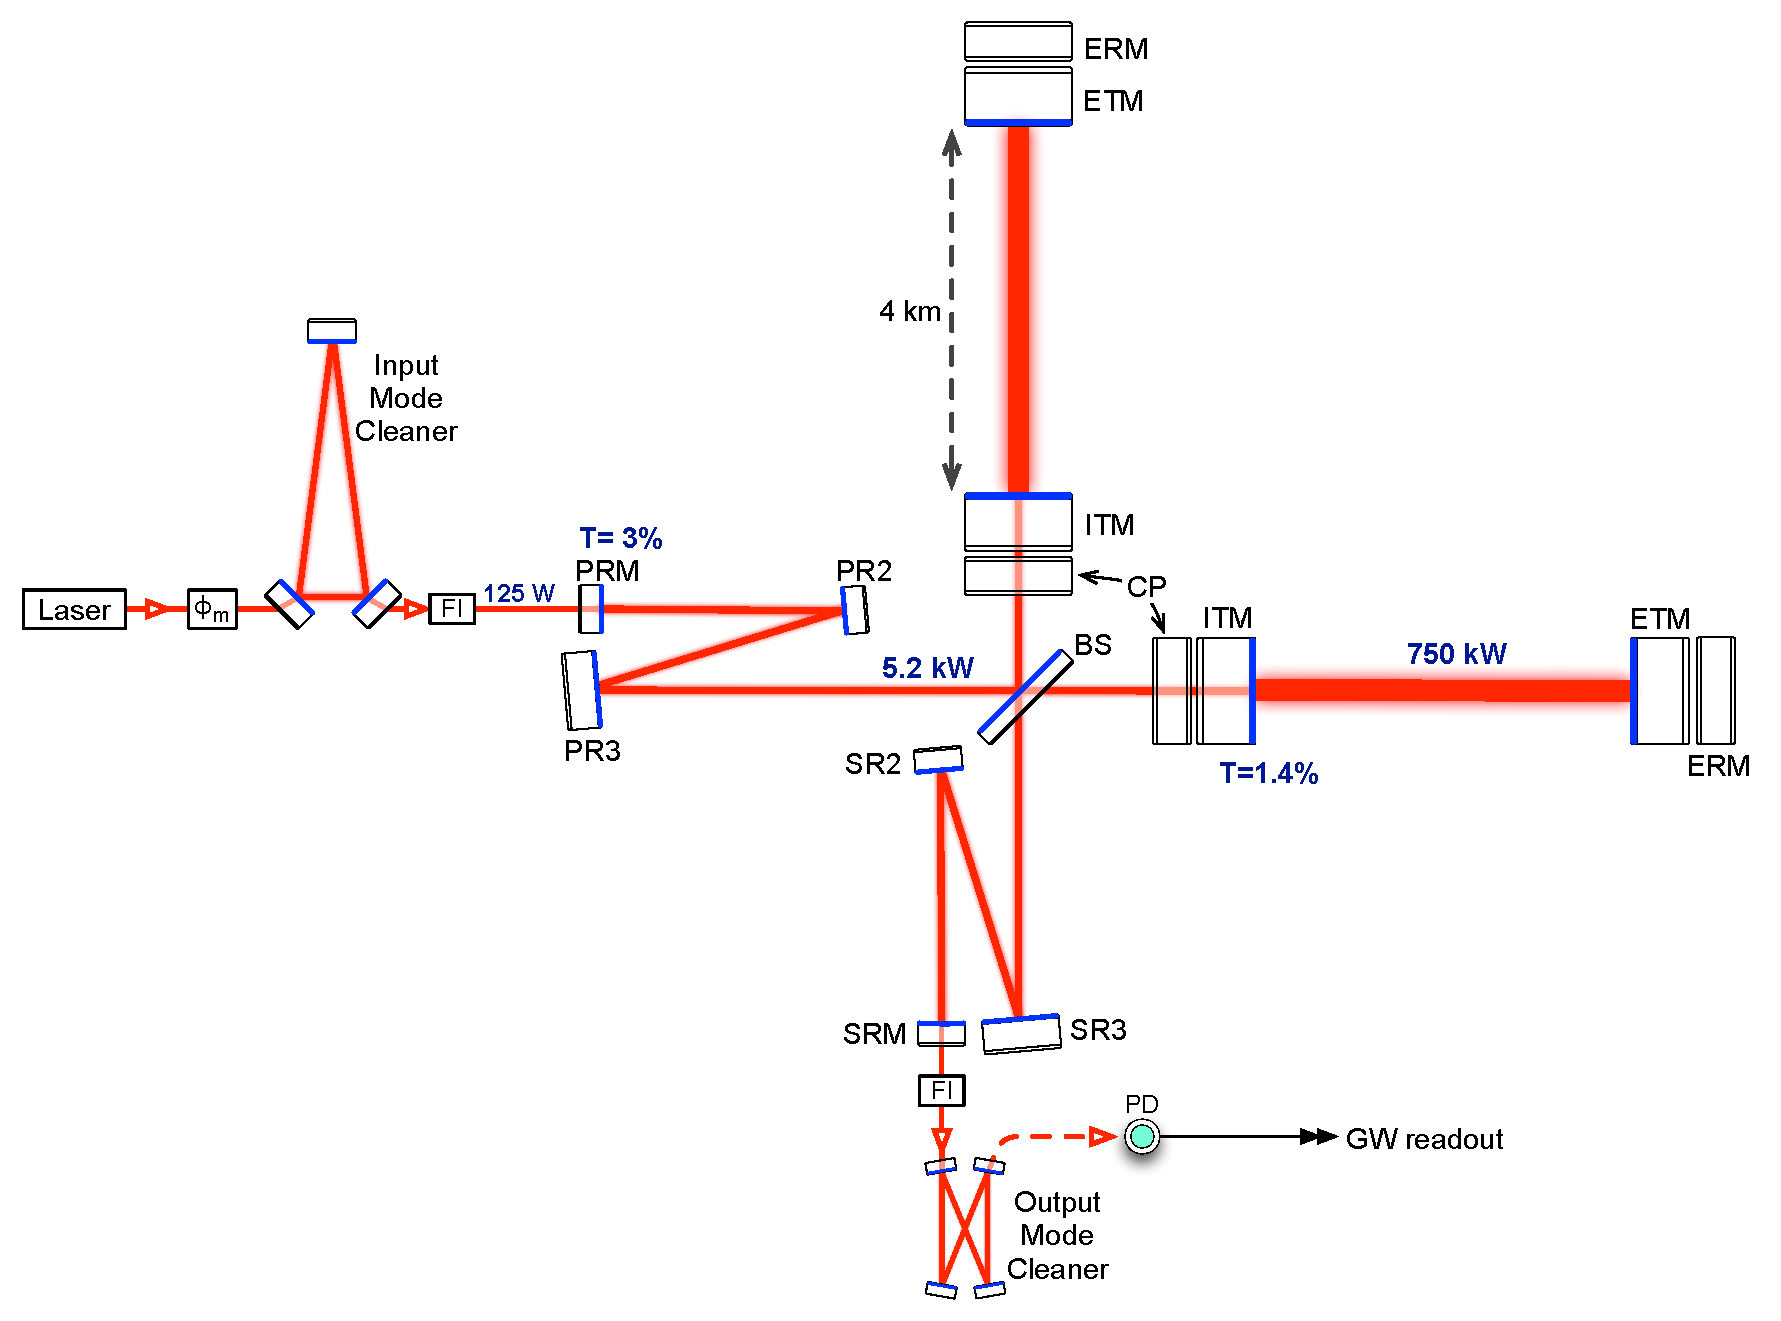
\includegraphics[width=\textwidth]{images/1_general_relativity/IFOdiagram.pdf}
   \caption{\label{fig:IFO}A more complex interferometer diagram \cite{aLIGO:2015}: The Fabry-Perot cavities are formed by the input test mass (ITM) and end test mass (ERM) of each arm, the power recycling mirrors (PRM, PR2, PR3) appear prior to the beam splitter (BS)}
\end{figure}

Within the reference frame of the beam splitter and in the absence of \gws, the distance each laser travels up the arms is equal so that upon returning to the beam splitter, we see a constant interference pattern in the photodetector.
As a \gw propagates through the detector the beam splitter remains at rest but the mirrors at the end of each arm move (in our cartesian coordinate system), the lengths of the arms are now different and the recombination of the two beams will produce a phase difference upon returning back to the beam splitter \cite{thorne_lecture}.


%---% Searches %---%
\chapter[Searching for Gravitational Waves from Compact Binary Coalescences]{\label{chapter:2-searches}Searching for Gravitational Waves from Compact Binary Coalescences}
\chapterquote{``This chapter needs a quote'' - Arthur Tolley}
%%% CBC SEARCH %%%
% Gravitational Wave data
%    h = s + n
% Signal Model
%    Waveforms
% Noise Model
%    PSD
% Search Methods
%    Matched Filter
%    Phase Maximisation
%    Template Bank
%    Signal Consistency Tests
%    Exponential Noise Model
%    PSD Variation
%    Coincidence Tests
%        Simple One
%        PhaseTD
%    Ranking Statistic
% PyCBC
%    Offline vs Live
%    Low-Latency Detection
%    SNR Optimisation
% Gravitational-Wave Observations to date



% Chapter Introduction

\Gwadj search pipelines, such as PyCBC, play a critical role in analysing data from detectors to identify \gwadj signals, both in real-time (live) and in post-processing (offline). This chapter develops the theoretical foundation for these search pipelines and explores the techniques employed in \gwadj detection. Emphasis is placed on the PyCBC pipelines---PyCBC Offline and PyCBC Live---both of which were extensively utilised and further developed as part of this thesis.

\section{\label{2:sec:gw-data}\Gwadj data}

\Gwadj observatories produce a dimensionless strain time-series, $s(t)$, which is composed of detector noise, $n(t)$, and, when present, an astrophysical \gwadj signal, $h(t)$
%
\begin{equation}
    s(t) =
    \begin{cases}
        n(t), & \text{if no signal is present}, \\
        n(t) + h(t), & \text{if a signal is present}.
    \end{cases}
\end{equation}
%
The primary objective of \gwadj search pipelines is to extract $h(t)$ from $s(t)$, detecting the astrophysical signal from inside the background noise.

\section{\label{2:sec:search-methods}Searching through \gwadj data}

Detecting \gws from \cbcs requires sophisticated search methods capable of sifting through vast amounts of data collected by \gwadj detectors. This section details the search techniques used to identify and characterize \gwadj signals. There many pipelines which search for \gws~\cite{pipelines} and in this section we will focus on the PyCBC search~\cite{PyCBC:2016, PyCBC:2017, PyCBC_package:2021}

We begin with the single detector search techniques to identify potential \gwadj events and then detail the tests and techniques used to combine single detector detections to identify coincidentally found \gwadj signals.

\subsection{\label{2:sec:matched-filter}Matched filtering}

% Use Jolien's book
Detecting \gws relies on being able to distinguish between data that contains a \gwadj signal, \( s(t) = n(t) + h(t) \), and data which is only noise, \( s(t) = n(t) \). We must construct an optimal detection statistic which expresses the value of the probability that the data contains a known signal. The optimal detection statistic is found by computing the ratio of the probability that the data contains the signal (hypothesis $\mathcal{H}_{1}$) to the probability that the data is pure noise (the null hypothesis $\mathcal{H}_{0}$)
%
\begin{equation}
    \Lambda = \frac{P(s|\mathcal{H}_{1})}{P(s|\mathcal{H}_{0})},
\end{equation}
%
where \( \Lambda \) is the likelihood ratio that serves as the detection statistic, \( P(s|\mathcal{H}_{1}) \) is the probability that the data contains the signal, and \( P(s|\mathcal{H}_{0}) \) is the probability that the data is pure noise. It is natural to use probability densities due to the detection process involving continuous data and not discrete events
%
\begin{equation}
    \Lambda = \frac{p(s|\mathcal{H}_{1})}{p(s|\mathcal{H}_{0})},
    \label{2:eq:likelihood_ratio}
\end{equation}
%
where \( p(s|\mathcal{H}_{1}) \) is the probability density that the data contains the signal, and \( p(s|\mathcal{H}_{0}) \) is the probability density that the data is pure noise.

If the detector noise is Gaussian we can compute the probability densities
%
\begin{align}
    p(s|\mathcal{H}_{0}) &\propto {\rm e}^{-(s|s)/2}, \\ 
    p(s|\mathcal{H}_{1}) &\propto {\rm e}^{-(s-h|s-h)/2},
\end{align}
%
and the likelihood ratio (equation~\ref{2:eq:likelihood_ratio})
%
\begin{equation}
    \Lambda(\mathcal{H}_{1}|s) = \frac{{\rm e}^{-(s-h|s-h)/2}}{{\rm e}^{-(s|s)/2}} = {\rm e}^{(s|h)}{\rm e}^{-(h|h)/2},
\end{equation}
%
where it is sensible to take the logarithm to obtain the log-likelihood ratio
%
\begin{equation}
    \log \Lambda(\mathcal{H}_{1}|s) = (s|h) - \frac{(h|h)}{2}.
    \label{2:eq:log_likelihood_ratio}
\end{equation}
%
From equation~\ref{2:eq:log_likelihood_ratio} we can see that the likelihood ratio depends only on the data through the inner product of $s$ and $h$. We define the noise-weighted inner product between two time series $s(t)$ and $h(t)$ as
%
\begin{equation}
  (s | h) = 4 \Re \int^{\infty}_{0} \frac{\tilde{s}(f) \tilde{h}^*(f)}{S_n(f)} df,
  \label{2:eqn:inner_product}
\end{equation}
%
where a tilde denotes a Fourier transformed version of the variable and where $S_n(f)$, represents the one-sided power spectral density (PSD) of the data, defined as
%
\begin{equation}
  \langle \tilde{s}(f) \tilde{s}(f^\prime) \rangle = \frac{1}{2} S_n(f) \delta(f - f^\prime) \;,
  \label{2:eqn:psd}
\end{equation}
%
where angle brackets denote an average over noise realisations and $\delta$ is the Dirac delta function. This inner product is the optimal detection statistic and is known as the \textit{matched filter}, effectively a noise-weighted correlation between the known signal and the data.

Since we are interested in evaluating the presence of a signal in the data, it is useful to define the \textit{signal-to-noise ratio} (SNR), \( \rho \), which quantifies how strong the signal is relative to the background noise. The SNR is defined as~\cite{FINDCHIRP:2012}
%
\begin{equation}
    \rho = \frac{(s|h)}{\sqrt{(h|h)}}.
    \label{2:eq:snr}
\end{equation}
%
This expression indicates how well the signal correlates with the data, relative to the noise level in the detector. When the detector contains a real signal a high SNR corresponds to a stronger, more detectable signal, whereas a low SNR indicates a weak signal buried in the noise. We will use the SNR value as the detection statistic moving forward.

\subsection{\label{2:sec:snr_timeseries}Signal-to-noise ratio over time}

We have assumed that we know all the parameters of the signal we are searching for, this is not likely for real \gwadj signals. We will begin to build up a more robust search in which we know very few of the initial \gwadj signal parameters. First, we consider the case of a signal that has a known waveform but an unknown amplitude and arrival time. We can describe the true signal as
%
\begin{equation}
    h(t) = A g(t - t_{0}),
\end{equation}
%
where A is the unknown amplitude of the signal, $t_{0}$ is the unknown arrival time and $g(t)$ is the known waveform. We can take the Fourier transform of this signal
%
\begin{equation}
    \tilde{h}(f) = A \tilde{g}(f) {\rm e}^{-2\pi i f t_{0}},
\end{equation}
%
and obtain the matched filter using equation~\ref{2:eqn:inner_product} to be
%
\begin{equation}
    (s|h) = 4 A \Re \int^{\infty}_{0} \frac{\tilde{s}(f) \tilde{h}^*(f)}{S_n(f)} {\rm e}^{2\pi i f t_{0}} df.
\end{equation}
%
From this we can define
%
\begin{align}
    (s|h) &= A x(t_{0}) \quad \text{where}, \\
    x(t) &= 4 \Re \int^{\infty}_{0} \frac{\tilde{s}(f) \tilde{g}^*(f)}{S_n(f)} {\rm e}^{2\pi i f t} df.
\end{align}
%
$x(t)$ is a time series representing the matched filter at any arrival time $t$. From this we can define an SNR time series $\rho(t)$ containing information about the SNR value at each point in time. To find the maximum likelihood detection statistic we simply find the largest value of $\rho(t)$ which will correspond to the amplitude and will reveal the previously unknown arrival time $t_{0}$.

\subsection{\label{2:sec:phase-maximisation}Phase maximisation}

The phase of the \gwadj signal is another unknown parameter. In section~\ref{1:sec:fourier_transform_chirp} we give a signal of the form
%
\begin{equation}
    h(t) = A(t) \cos\left(\Phi(t)\right),
\end{equation}
%
and can include an additional phase offset, $\phi_{0}$, to account for the random orientation and sky position of the binary
%
\begin{equation}
    h(t) = A(t) \cos\left(\Phi(t) + \phi_{0}\right).
    \label{2:eq:phase_signal_model}
\end{equation}
%
We can maximise over this phase offset using the matched filter by rewriting our signal as
%
\begin{equation}
    h(t) = h_{0}(t) \cos(\phi_{0}) + h_{\pi/2}(t)\sin(\phi_{0}),
\end{equation}
%
where $h_{0}(t)$ and $h_{\pi/2}(t)$ are realisations of equation~\ref{2:eq:phase_signal_model} where the phase offset has been set equal to $0$ and $\frac{\pi}{2}$ respectively~\cite{IHOPE:2012zx}.

We can then calculate $\rho^{2}$ using these two new signals to maximise over the phase
%
\begin{equation}
    \underset{\Phi}{\text{max}}(\rho^{2}(t)) = \frac{(s|h_{0})^{2} + (s|h_{\pi/2})^2}{(h_{0}|h_{0})},
    \label{2:eq:phase_max}
\end{equation}
%
having made the assumption that $\tilde{h}_{\pi/2}(f) = i\tilde{h}_{0}(f)$ which is true for frequency domain waveforms with the stationary phase approximation~\cite{Droz:1999}. We take the square root of equation~\ref{2:eq:phase_max} to get the SNR where phase has been maximised over
\begin{equation}
    \rho = \sqrt{\underset{\Phi}{\text{max}}(\rho^{2}(t))}.
\end{equation}

\subsection{\label{2:sec:template-bank}Template bank}

We have demonstrated that the matched filter can be used to analytically and efficiently maximise over the amplitude, time of arrival and phase of a known signal. We acknowledge that for a real search for \gws we will not know the $15$ parameters of the signal. The search is performed by creating many realisations of the \gwadj signal and searching over the data with each of them. However, we need to discuss how the realisation parameter values are chosen to ensure a sufficiently covered parameter space.

When a signal is found by a template\footnote{A realisation of the \gwadj signal waveform.} with parameters not equal to the true values we will expect to see a fraction loss in the expected SNR. The closer the template parameters are to the signal parameters, the closer to the maximum SNR we will see. 

We can define a signal with parameters $\lambda$
%
\begin{equation}
    h(t) = \rho u(t;\lambda),
\end{equation}
where $\rho$ is the expected SNR value with the true template. If we have a template with parameters $u(t;\lambda + \Delta \lambda)$, the expected SNR when matched filtering the signal with the template will be
%
\begin{equation}
    \rho^{\prime} = (h|u(\lambda + \Delta \lambda)) = \rho(u(\lambda)|u(\lambda + \Delta \lambda)),
\end{equation}
%
and we can see therefore that the expected fractional loss in the expected SNR is
%
\begin{equation}
    \frac{\rho - \rho^{\prime}}{\rho} = 1 - (u(\lambda)|u(\lambda + \Delta \lambda)) = 1 - \mathcal{A},
\end{equation}
%
where we can define $\mathcal{A}$ as the ambiguity function
%
\begin{equation}
    \mathcal{A}(\lambda;\lambda + \Delta \lambda) := (u(\lambda)|u(\lambda + \Delta \lambda)),
\end{equation}
%
which tells us how well our nearby template matches to the true signal\footnote{Templates are assumed to be normalised such that $(u(\lambda)|u(\lambda)) = 1$.}. If the ambiguity value is large then we have a small fraction loss and the template is a good match to the true signal, if the value is small then the template is a poor description of the signal template.

% CHANGE ALL OF THIS TO BE NOT METRIC BASED

$\lambda$ contains both the \textit{intrinsic} and \textit{extrinsic} parameters of the signal, we can define the \textit{overlap} between two templates $h_{1}$ and $h_{2}$ considering only the intrinsic parameters,
%
\begin{equation}
    \mathcal{O}(h_{1}, h_{2}) := (h_{1} | h_{2}) = \frac{(h_{1} | h_{2})}{\sqrt{(h_{1} | h_{1})(h_{2} | h_{2})}}.
\end{equation}
%
For a signal $h_{1}$, the overlap represents the fraction of SNR recovered by matched filtering the signal with template $h_{2}$. The match is then the overlap which has been maximised over time of arrival and phase~\cite{Harry_Lundgren:2012}
%
\begin{equation}
    \mathcal{M}(h_{1}, h_{2}) = \underset{\phi_0, t_{c}}{max}(\hat{h}_{1}|\hat{h}_{2}(\phi_{c}, t_{c})).
\end{equation}
%
We can then construct a bank of templates with a requirement that any signal, when matched filtered by the whole bank, can be recovered with a maximum of $3\%$~\cite{Owen_Sathya:1999} loss. This corresponds to a mismatch, $1 - \mathcal{M}$, of $0.03$, at least one template in the template bank must have a maximised overlap of at least $0.97$ with the true signal waveform.

\subsection{\label{2:sec:signal-consistency}Signal consistency tests}

We have described the matched filter as the optimal detection statistic in stationary Gaussian noise when searching for a known signal. While we have dealt with the case of an unknown signal we now consider the case where the detector noise is not Gaussian. Within the detector data we have many instances of short duration bursts of excess power that are non-Gaussian, commonly called `glitches'~\cite{LIGO_data_quality:2015}.

Glitches produce large SNRs in the matched filter even when they do not share the same morphological characteristics. To combat this we use signal consistency tests, which are able to discriminate between glitches and signal based on the distribution of the power present in the detector data.

We know the expected time and frequency evolution of a \gwadj signal using our waveform models. The time-frequency waveform consistency test described in~\cite{Allen_Chi:2005} (the Allen $\chi^{2}$ test) divides the signal template into $p$ sub-templates such that each of the sub-templates contributes equally to the total SNR
%
\begin{equation}
    4 \int^{f_{1}}_{0}\frac{\tilde{s}(f) \tilde{h}_{1}(p)^*(f)}{Sn(f)}df = 4 \int^{f_{2}}_{f_{1}}\frac{\tilde{s}(f) \tilde{h}_{2}(p)}{Sn(f)}df = ... =  4 \int^{\inf}_{f_{p-1}}\frac{\tilde{s}(f) \tilde{h}_{p}(f)}{Sn(f)}df ,
\end{equation}
%
where $\tilde{s}(f)$ is the data and $\tilde{h_{p}}(f)$ the sub-templates from discrete non-overlapping frequencies.

To calculate the divergence from the expected time-frequency distribution we can calculate the chi-squared value evaluated at some time, $t_{0}$, using
%
\begin{equation}
    \chi^{2}(t_{0}) = \sum^{p}_{i=1} \left(\frac{\rho}{\sqrt{p}} - \rho_{bin, i}\right),
\end{equation}
%
where $p$ is the number of sub-templates (bins), $\rho$ is the SNR for the full template matched-filtered with the data and $\rho_{bin}$ is the SNR found when matched filtering the sub-template and the data. The $\chi^{2}$ value will be small for data containing the true signal but will be large when the SNR found in some bins is different from the expected SNR, notably in the presence of a glitch with power distribution that does not match the signal.

If the data noise is Gaussian the $\chi^{2}$ value will be $\chi^{2}$ distributed with $2p - 2$ degrees of freedom, therefore, we use the reduced-$\chi^{2}$ value which will evaluate close to $1$ for the true signal template
%
\begin{equation}
    \chi_{r}^{2} = \frac{\chi^{2}}{2p-2}.
    \label{2:eq:reduced_chisq}
\end{equation}
%
Another $\chi^{2}$ test used by \gwadj searches is the sine-Gaussian $\chi^{2}$ test~\cite{PyCBC_sg:2018} which searches for excess power in the frequencies above the expected frequency range of the signal.

These two $\chi^{2}$ tests are used to re-weigh the SNR of the matched filter, first the Allen $\chi^{2}$ test is applied~\cite{McIsaac_Chi:2022}
%
\begin{equation}
    \rho =
    \begin{cases}
        \hat{\rho}, & \text{if \,} \chi^{2}_{r} \le 1, \\
        \rho\left[(1 + (\chi^{2}_{r})^{3}) /2\right]^{-\frac{1}{6}}, & \text{if \,} \chi^{2}_{r} > 1,
    \end{cases}
\end{equation}
%
then the sine-Gaussian $\chi^{2}$ test is applied
%
\begin{equation}
    \hat{\rho}_{sg} =
    \begin{cases}
        \hat{\rho}, & \text{if \,} \chi^{2}_{r} \le 4, \\
        \hat{\rho}\left(\chi^{2}_{r, sg})/4\right)^{-\frac{1}{2}}, & \text{if \,} \chi^{2}_{r} > 4.
    \end{cases}
\end{equation}
%
We define a detection threshold such that a template found at a time with SNR above the threshold will be considered for consideration as a \gwadj signal, we call these detections `triggers'. The re-weighted SNR is used to rank detector triggers from single detector matched filters.

\subsection{\label{2:sec:auto-gating}Auto-gating}

Some glitches are too loud to be suppressed by the signal consistency tests and will produce very large SNR values when matched-filtered with the template bank. Glitches which resemble delta-functions can produce not only a very high SNRs but can also cause a \textit{ringing} effect where the matched filter will continue to produce high SNR triggers for a short time.

These glitches are identified by looking for excess power in the whitened\footnote{Whitened data has a flat power spectral density with no frequency-dependent noise.} data and are handled by applying a windowing function around the data. This process is known as \textit{gating} and the window is applied such that a smooth transition between data and zeroing is made to avoid discontinuities in the data which can introduce more data artefacts. Figure~\ref{2:fig:autogating} shows an example of a glitch which has been gated.
%
\begin{figure}
    \centering
    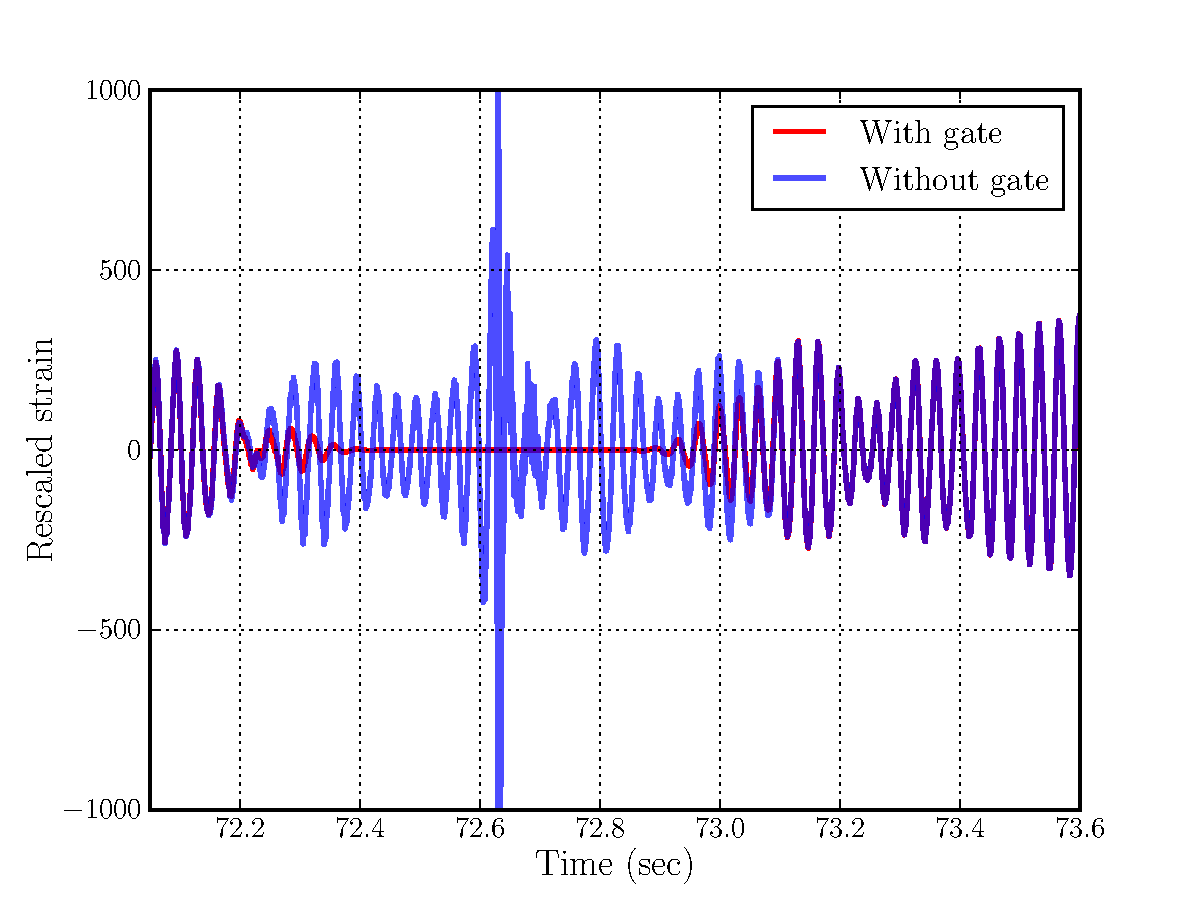
\includegraphics[width=0.9\linewidth]{images/2_searches/autogating.pdf}
    \caption{Gating a very loud noise transient. The detector strain has been rescaled by a factor of $10^{21}$ and the glitch has a peak magnitude over $5,000$. The blue line shows the data before applying the Tukey window and the red shows the data after applying the Tukey window. Note the smooth decrease in data amplitude at the edges of the windowing function. Image taken from~\cite{PyCBC:2016}.}
    \label{2:fig:autogating}
\end{figure}
%

Gating occurs automatically in \gwadj searches in a process called `auto-gating'. Auto-gating in PyCBC Live zeroes only $0.25$ seconds of data with a taper of $0.25$ seconds on either side.

\subsection{\label{2:sec:coincidence-test}Coincidence tests}

Non-Gaussian transients in our detector data lead to greatly increased possibility for a \gwadj detector to report detections of \gwadj signals caused by non-astrophysical sources. If, after our signal-consistency tests, a glitch has a large SNR we are unable to make a distinction between it and a real event.

In terms of the optimal detection statistic we must include further components which can reject glitches while ensuring we continue to detect all possible real events. The most powerful method for confirming the detection in one detector is the coincidental detection of the same signal in another detector. We call this a \textit{coincidence test}; the requirement that for a signal to be considered real it must have been observed in multiple detectors.

In a two detector example, for example LIGO-Hanford and LIGO-Livingston, the signal seen by both detectors will not be exactly the same. The detectors are located approximately $3,000 \, \text{km}$ from one another, (figure~\ref{2:fig:observatories}) and we know \gws propagate at the speed of light (section~\ref{1:sec:keplerian_derivation}).
%
\begin{figure}
    \centering
    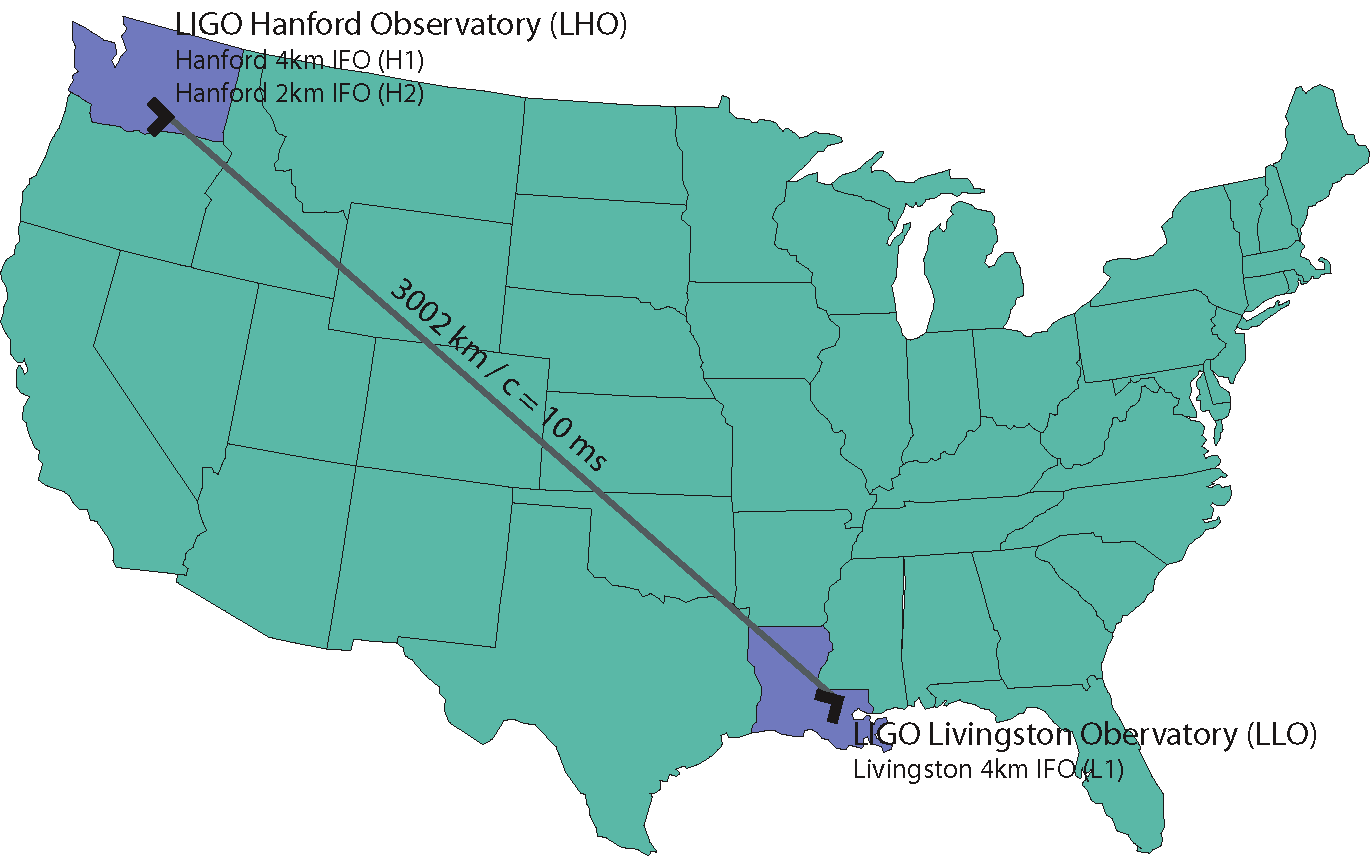
\includegraphics[width=0.8\linewidth]{images/2_searches/observatories.png}
    \caption{The two LIGO detectors locations and orientations, separated by approximately $3,000 \, \text{km}$. Taken from~\cite{Brown_Thesis:2004}.}
    \label{2:fig:observatories}
\end{figure}
%
Therefore, we can expect a maximum delay between single-detector detections of $10 \, \text{ms}$. For the coincidence test we must allow a window between single detector triggers of this light travel time. Additionally, it is only sensible to make the requirement that the intrinsic parameters of the two single detector triggers are the same, i.e. they have seen the same gravitational waveform.


\subsection{\label{2:sec:ranking-statistic}Ranking statistic}

Finally, we can combine all these components to create a ranking statistic which we treat as the optimal detection statistic for identifying \gwadj signals from \gwadj detector data. The optimal detection statistic is the likelihood ratio~\cite{Biswas:2012}
%
\begin{equation}
    \Lambda(\vec{\kappa}) = \frac{r_{n}(\vec{\kappa})}{r_{s}(\vec{\kappa})},
\end{equation}
%
where $\vec{\kappa}$ is a set of parameters
%
\begin{equation}
    \vec{\kappa} = \left\{ \left[\rho_{d}, \chi^{2}_{d}, \chi^{2}_{d, sg}, \sigma_{d}\right], \vec{\theta}, \left[\mathfrak{A}_{d_{1}d_{2}}, \delta t_{d_{1}d_{2}}, \delta\phi_{d_{1}d_{2}}\right] \right\}.
\end{equation}
%
$\vec{\kappa}$ contains three categories of parameter: first, the single detector trigger parameters for each detector $d$, SNR, Allen-$\chi^{2}$, sine-Gaussian $\chi^{2}$ and template sensitivity ($\sigma_{d}$); next, the intrinsic template parameters $\vec{\theta}$ and; the coincident trigger parameters, amplitude ratio ($\mathfrak{A}_{ab}$), time of arrival difference ($\delta t_{ab}$) and phase difference ($\delta \phi_{ab}$) between two detectors $d_{1}$ and $d_{2}$.

The likelihood ratio is expressed as a ratio of event rate densities~\cite{PyCBC_global:2020} where
%
\begin{equation}
    r_{s}(\kappa) = \frac{\text{Number of signal events}}{\text{Volume} \times \text{Time}},
\end{equation}
%
\begin{equation}
    r_{n}(\kappa) = \frac{\text{Number of noise events}}{\text{Volume} \times \text{Time}}.
\end{equation}
%
Again, it is natural to use the log-likelihood ratio due to the order of magnitude difference between the event rate densities
%
\begin{equation}
    R(\vec{\kappa}) = \log \Lambda(\vec{\kappa}) = \log r_{s}(\vec{\kappa}) - \log r_{n}(\vec{\kappa}).
\end{equation}
%
We call the log-likelihood detection statistic the ranking statistic which is constructed from a noise model and signal model. The PyCBC noise and signal models have changed over the course of the \gwadj search history. For this reason we will focus primarily on the models used in one of the first searches for \cbcs---\texttt{ihope}~\cite{IHOPE:2012zx}

\subsubsection{\label{2:sec:ihope}ihope}

The \texttt{ihope} search pipeline ranked single detector triggers by their SNR and $\chi^{2}$ values to create a re-weighted SNR, $\hat{\rho}$ for each detector. The ranking statistic noise model used by the \texttt{ihope} search pipeline was a simple quadrature sum of single detector re-weighted SNRs
%
\begin{equation}
    \hat{\rho}^{2} = \sqrt{\hat{\rho}^{2}_{d_{1}} + \hat{\rho}^{2}_{d_{2}}}.
    \label{2:eq:IHOPE_noise_model}
\end{equation}
%
The \texttt{ihope} search pipeline had no signal model and so the ranking statistic was simply the noise model presented above. As detailed in~\cite{IHOPE:2012zx}, this ranking statistic was shown to `downrank' all triggers below a re-weighted SNR of $6$ in both a Gaussian noise simulation and the $5^{th}$ science run of LIGO~\cite{S5:2012}. We note that in this case there are $0$ real signals in the data and therefore this noise model has been applied to only noise triggers.

\subsection{\label{2:sec:background-estimation}Candidate event significance}

We can define some threshold at which a coincident trigger with ranking statistic value above this threshold can be preliminary considered to be a \gwadj event, we refer to these coincident triggers as \textit{candidates}. We define the \textit{significance} of the candidate use the \textit{false-alarm rate}. False alarms are coincident triggers that have been cause entirely by noise, with no astrophysical origin. The rate of false alarms depends on the search pipeline's response to detector noise and must be measured empirically.

The PyCBC search pipeline measures the false-alarm rate using `time slides'. As discussed in section~\ref{2:sec:coincidence-test}, a coincident trigger can only be formed if the triggers are within the light travel time window. Therefore, if a coincident is made between two single detector triggers outside of this window it \textbf{must} be caused by detector noise and not an astrophysical signal. To measure the background rate of coincident triggers we can take the triggers from the first detector and count all the coincidences made with the triggers from the second detector after shifting the time in the second detector by greater than the light travel time window. This ensures that any coincidences made cannot possibly have been due to a real signal because the coincidences will have occurred outside of the light travel time window. An example of a background coincidence by these time slides for the three detector case can be seen in figure~\ref{2:fig:timeslides}.
%
\begin{figure}
    \centering
    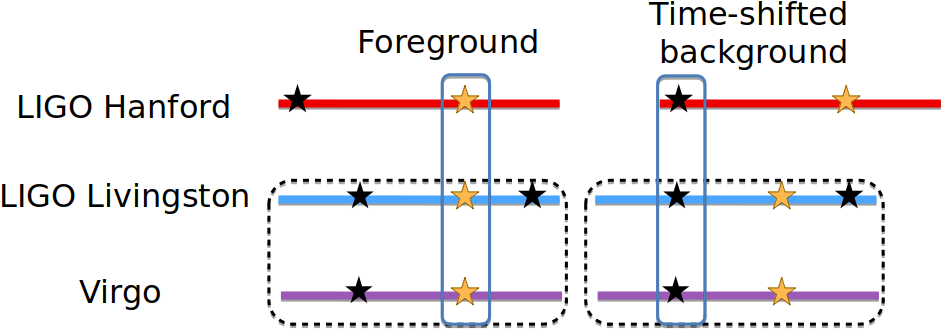
\includegraphics[width=0.9\linewidth]{images/2_searches/TimeslideExample.png}
    \caption{The time-sliding process carried out by the PyCBC search to generate a background distribution of candidate events. The foreground, real \gwadj event, is shown as a golden star and is the coincidence between three detectors with a single detector trigger in each which falls within the allowed light travel time of the detector network. The dashed black box indicates a time slide being made where two detectors have their data shifted by an interval greater than the allowed light travel time window to produce events which can only be caused by non-astrophysical noise sources. An example of a background event is shown as the three black stars in the blue box on the right image. Taken from~\cite{PyCBC_global:2020}.}
    \label{2:fig:timeslides}
\end{figure}
%

The time sliding procedure is repeated many times to produce a large sample of false-alarm coincidences which are used to compute the false-alarm rate as a function of the ranking statistic.

To measure the significance of each candidate event we assign a p-value. In our pipeline the p-value of a candidate event is the probability that there are one or more false-alarm event that have a ranking statistic value greater than or equal to the ranking statistic of the detector value, $p_{b} = P(R_{FA} \ge R_{CE})$. The p-values of candidates events are calculated under the null hypothesis that \textit{all} triggers are seen due to noise. To confidently claim the candidate event as real, we must demonstrate that the null hypothesis given the candidate event ranking statistic value is highly improbable (the p-value is small).

We can do this by measuring the number of noise background events, $n_{b}$, that have a ranking statistic value higher than the candidate event. If we do this for all ranking statistic values we can build up a mapping of ranking statistic to false-alarm rate. The function $n_{b}(R)$ gives the number of background events with a ranking statistic value higher than $R$, the ranking statistic value. The probability that one or more background events are found above $R$ given the observing time $T$ and the background time $T_{b}$ is~\cite{PyCBC:2016}
%
\begin{equation}
    p(\ge 1 \, \text{above} R|T, T_{b})_{0} = 1 - \exp \left[\frac{-T(1 + n_{b}(R))}{T_{b}}\right].
\end{equation}
%
The background time will equal $T_{b} = T^{2}/\delta$ where $\delta$ is the time-slide interval. We can produce a very large amount of background data from a relatively small period of observing data, fifteen days of coincident data with a time-slide interval of $0.1$ seconds allows us to measure false-alarm rates of $1$ in $200,000$ years.

Finally we can express the mapping of false-alarm rate to ranking statistic as
%
\begin{equation}
    \text{FAR}(R^{*}) = \int r_{n}(\vec{\kappa}) \Theta(R(\vec{\kappa}) - R^{*}) d^{n}\vec{\kappa},
    \label{2:eq:far_mapping}
\end{equation}
%
where $\Theta$ is the Heaviside step function
%
\begin{equation}
    \Theta(x) =
    \begin{cases} 
        0 & \text{if } x < 0 \\
        1 & \text{if } x \geq 0,
    \end{cases}
\end{equation}
%
and the false-alarm rate at the ranking statistic value $R^{*}$ is being calculated by integrating over all possible background events and summing up the events that have a ranking statistic greater than or equal to $R^{*}$, the ranking statistic threshold. The optimal ranking statistic will maximise the expected number of coincident events due to signals recovered above $R^{*}$.

\section{\label{2:sec:gw-pipelines}\Gwadj search pipelines}

We can develop the idea of a \gwadj search pipeline by describing the structure of the \texttt{ihope}~\cite{IHOPE:2012zx} search pipeline and how \gwadj events are identified from the initial \gwadj data using all the techniques described previously in this chapter.

\subsection{\label{2:sec:searching-for-gw-with-ihope}\texttt{ihope}}
The flow chart describing the structure of the \texttt{ihope} pipeline has been taken from the \texttt{ihope} paper and can be seen in figure~\ref{2:fig:ihope-flowchart}. We follow this flowchart in our description of the search pipeline.
%
\begin{figure}
    \centering
    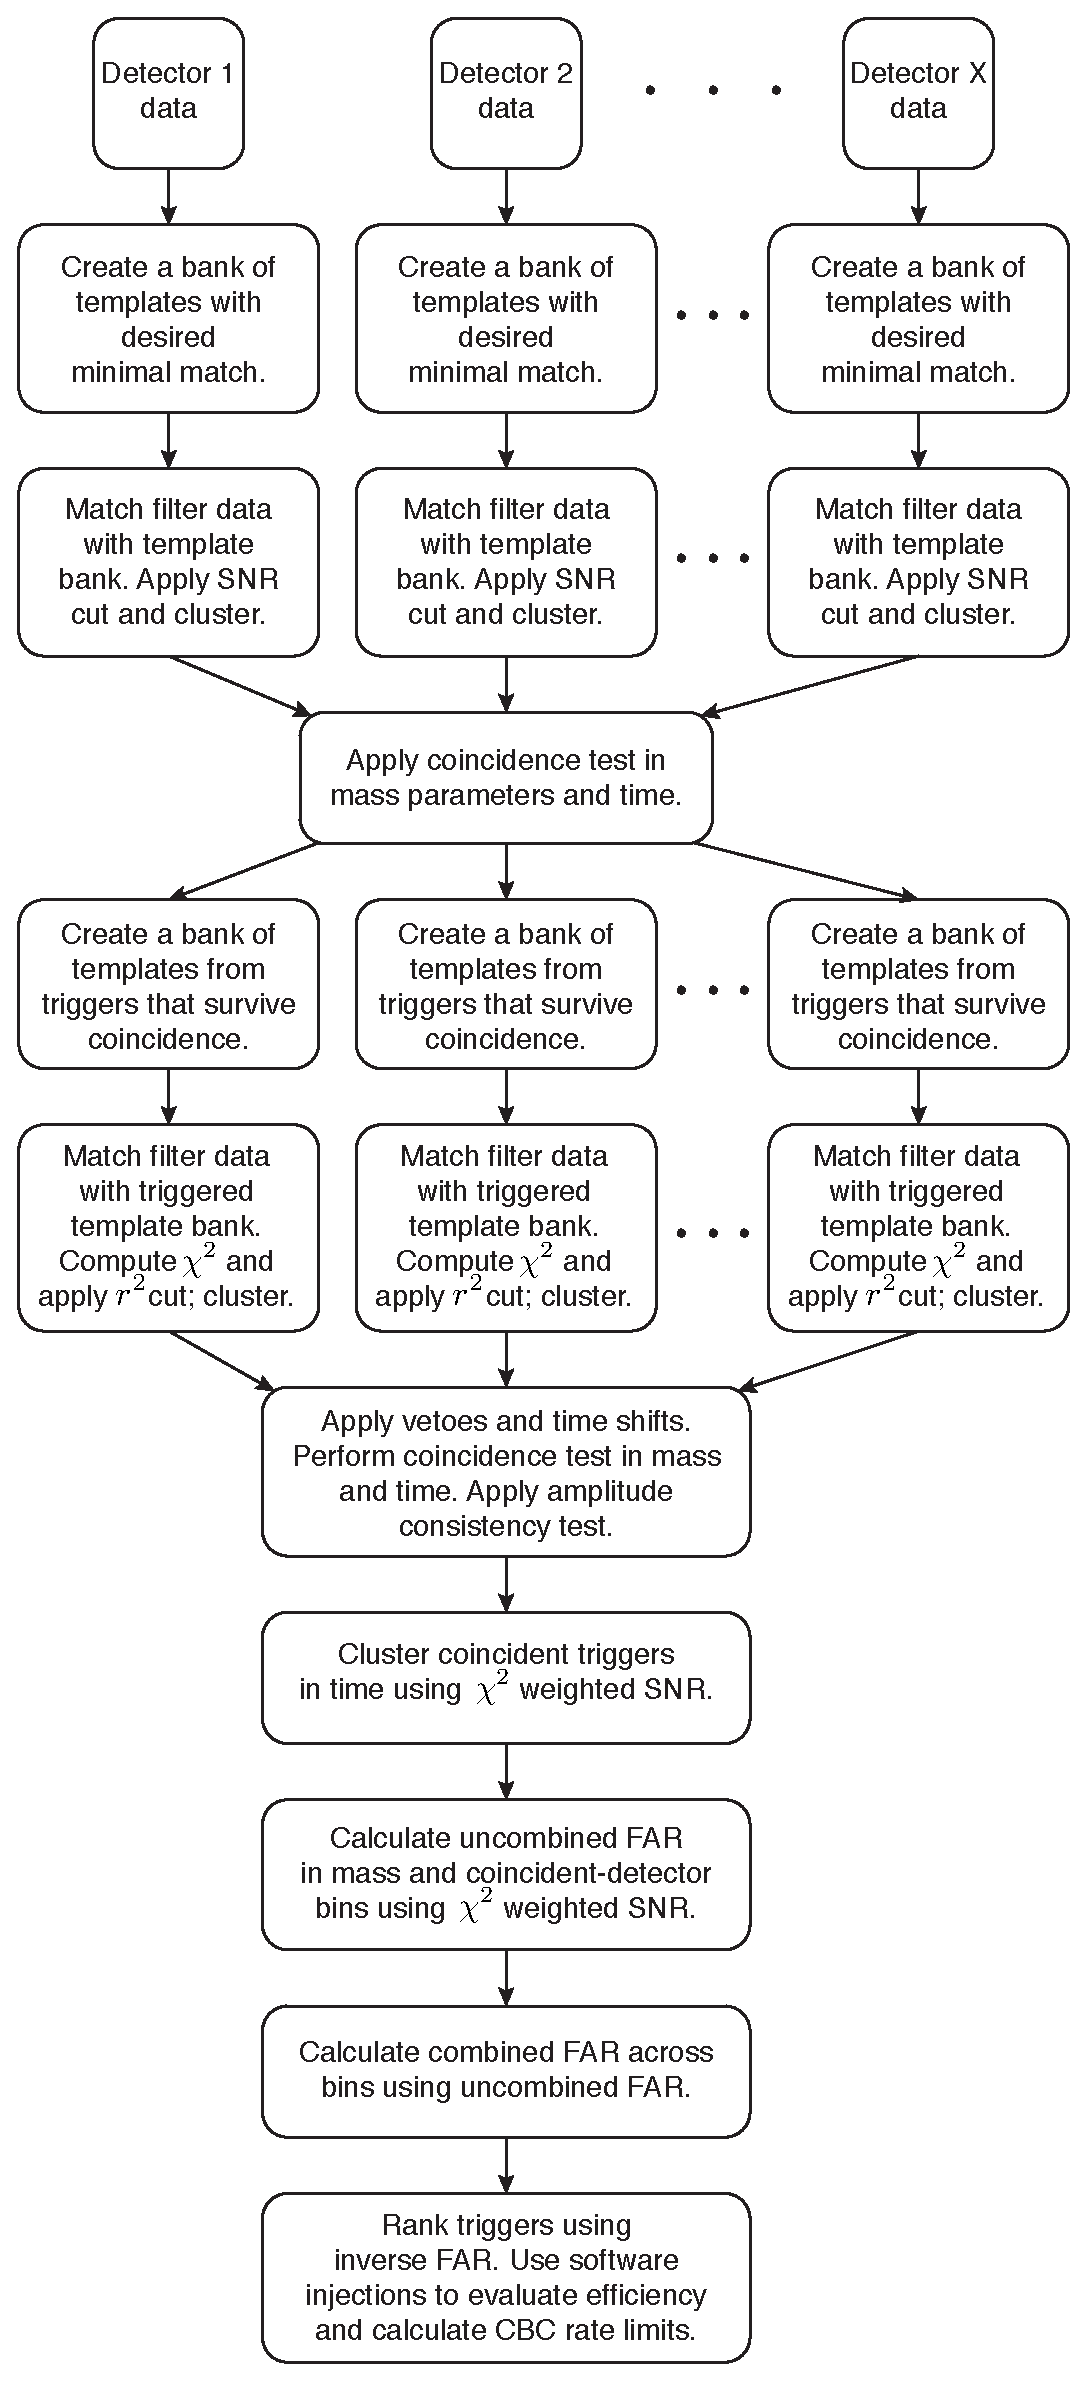
\includegraphics[width=0.6\linewidth]{images/2_searches/ihope_flowchart.pdf}
    \caption{The structure of the \texttt{ihope} search pipeline for \gws. Taken from~\cite{IHOPE:2012zx}.}
    \label{2:fig:ihope-flowchart}
\end{figure}

\subsubsection{Data conditioning}

Science data is \gwadj data that is collected during periods when the detector is functioning optimally and is capable detecting \gws. Science quality data is identified and split into $2048 \, \text{second}$ blocks, the LIGO data is initially sampled at $16,384 \, \text{Hz}$ and is down-sampled to $4096 \, \text{Hz}$ due to higher frequencies being dominated by detector noise and not containing any measurable \gwadj signal. The \texttt{ihope} pipeline also imposed a high-pass of $40 \, \text{Hz}$ due to low-frequency noise dominating below this. A $2048 \, \text{s}$ block will then be split into $15$ segments $256 \, \text{s}$ long where neighbouring segments overlap by $128 \, \text{s}$. The power spectral density (PSD) for a block of data is estimated by computing the PSD for each segment (equation~\ref{2:eqn:psd}), these are then median averaged to get the PSD for the whole block.

\subsubsection{Template bank generation}

A key consideration for \gwadj search pipelines is computational cost. A greater computational cost requires more time to analyse \gwadj data alongside greater monetary cost and carbon emission cost. The dominant cost for modelled searches is matched filtering. Therefore, the number of templates in the template bank is proportional to the computational cost of the search. The number of templates is tuned to balance a minimal loss in matched filter SNR with the computational cost.

The \texttt{ihope} template bank is placed with a minimum match of $0.97$ between any signal and the template bank. The loss in sensitivity due to this minimum match limit is equal to the minimum match$^{3}$ and is $\simeq 10\%$. Calculating the match between templates is the bank is simpler when using a flat parameter space such as ``chirp times'' $\tau_{0}$ and $\tau_{3}$~\cite{Droz:1999}
%
\begin{equation}
    \tau_{0} = \frac{5}{256\pi f_{low}\eta}\left(\frac{\pi G M f_{low}}{c^{3}}\right)^{-\frac{5}{3}},
\end{equation}
%
\begin{equation}
    \tau_{3} = \frac{5}{8 f_{low}\eta}\left(\frac{\pi G M f_{low}}{c^{3}}\right)^{-\frac{2}{3}},
\end{equation}
%
where $M$ is the total mass, $\eta$ is the symmetric mass ratio and $f_{low}$ is the lower frequency cutoff used in template generation. The template bank used by \texttt{ihope} during the later LIGO science runs was generated in the $\tau_{0}$-$\tau_{3}$ parameter space and contained approximately $6,000$ templates. The template bank depends on the noise curve of the data and therefore was generated per data block.
%
\begin{figure}
    \centering
    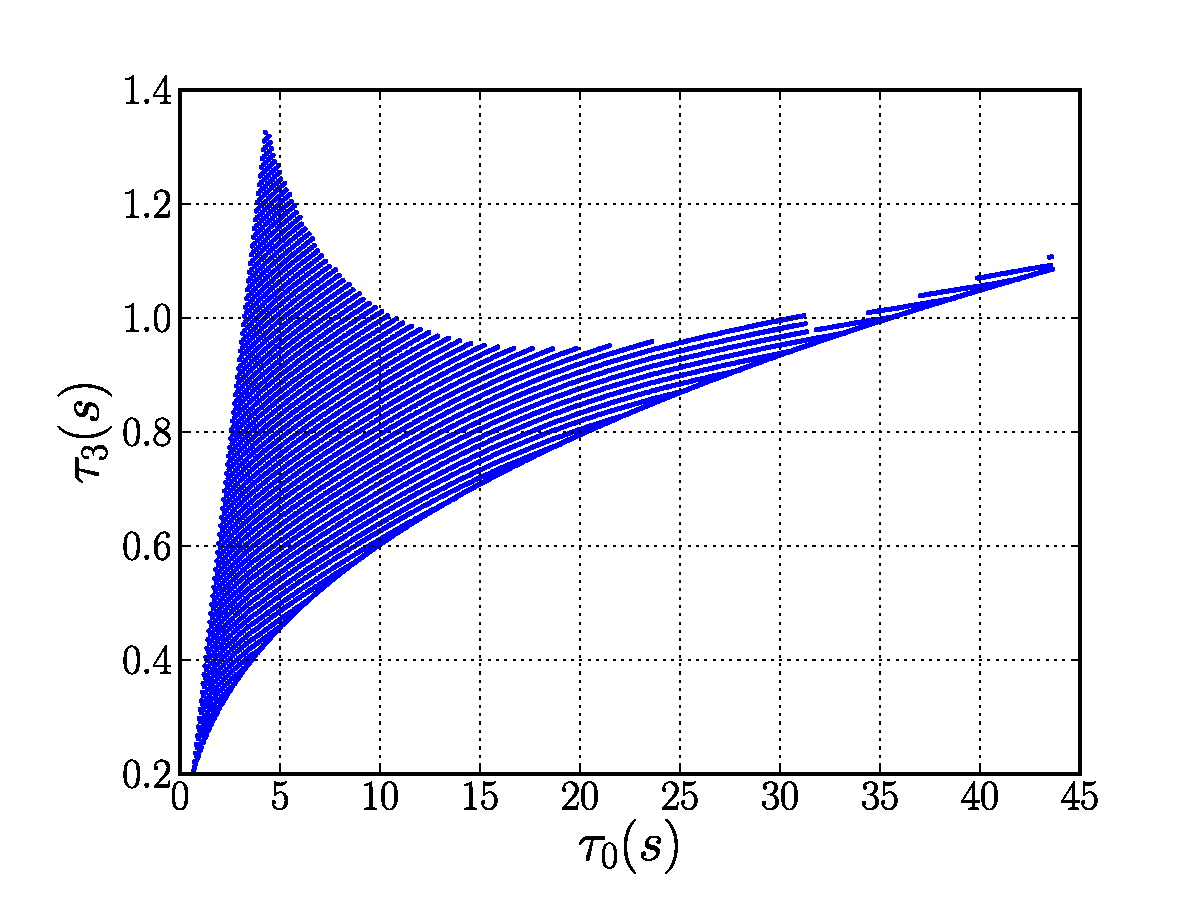
\includegraphics[width=0.75\linewidth]{images/2_searches/ihope_template_bank.pdf}
    \caption{An example of a template bank used by the \texttt{ihope} search pipeline that has been generated from a single block of data and has been created in the chirp time parameter space, $\tau_{0}$-$\tau_{3}$. Comprises of approximately $6,000$ templates. Taken from~\cite{IHOPE:2012zx}.}
    \label{2:fig:ihope-template-bank}
\end{figure}
%

\subsubsection{Matched filtering}

The matched filter between template bank and data is performed on each block of data to create a list of single detector triggers. Triggers are only stored if their matched filter SNR is greater than $5.5$. Suppose we have a trigger with an SNR of $10.0$, according to our template bank minimum match we should have at least one additional trigger (and indeed have many) above the SNR threshold for a nearby template. To prevent the recording of multiple triggers from different templates for the same candidate event we use a \textit{time clustering} algorithm which selects and keeps only the highest SNR trigger in a predefined time window. Another clustering algorithm, called \textit{TrigScan}, is employed to trigger across the template bank to prevent the triggering of a loud glitch in one region of the template bank from subduing a real signal trigger in a completely different region.

\subsubsection{Coincidence tests}

Single detector triggers are combined and evaluated based on their trigger times and template parameters, triggers that have been found within the maximum light travel time between the two detectors ($10 \, \text{ms}$ for LIGO-Hanford and LIGO-Livingston) with similar masses can be considered to originate from the same \gwadj signal~\cite{Robinson:2008}. The result of this process is a list of coincident triggers found with SNR above the threshold in two or more detectors with consistent template parameters across detectors.

\subsubsection{Matched filter again with signal consistency tests}

We note that this method has been heavily disfavoured in more modern search pipelines but we explain it briefly for completeness. The intention of the second template bank search is to save computational processing power used for the signal consistency tests.

The templates responsible for the coincident triggers found by the initial matched filter and coincidence test are used to create a \textit{triggered template bank} which is used to matched filter the data again. This time the $\chi^{2}$ test~\cite{Allen_Chi:2005} and an $r^{2}$ test are performed alongside consistency in relative signal amplitude and \textit{data-quality vetoes}.

The $\chi^{2}$ test values are calculated for each new SNR trigger found by the triggered template bank (equation~\ref{2:eq:reduced_chisq}). The \( r^{2} \) test assesses the sharpness of the SNR peak surrounding a large SNR trigger, under the premise that real \gwadj signals will exhibit a distinct peak, while non-astrophysical glitches will display a broader structure. The test counts the number of samples above a specified SNR threshold. An example of the SNR time series from a loud signal can be seen in figure~\ref{2:fig:ihope-snr-timeseries}.
%
\begin{figure}
    \centering
    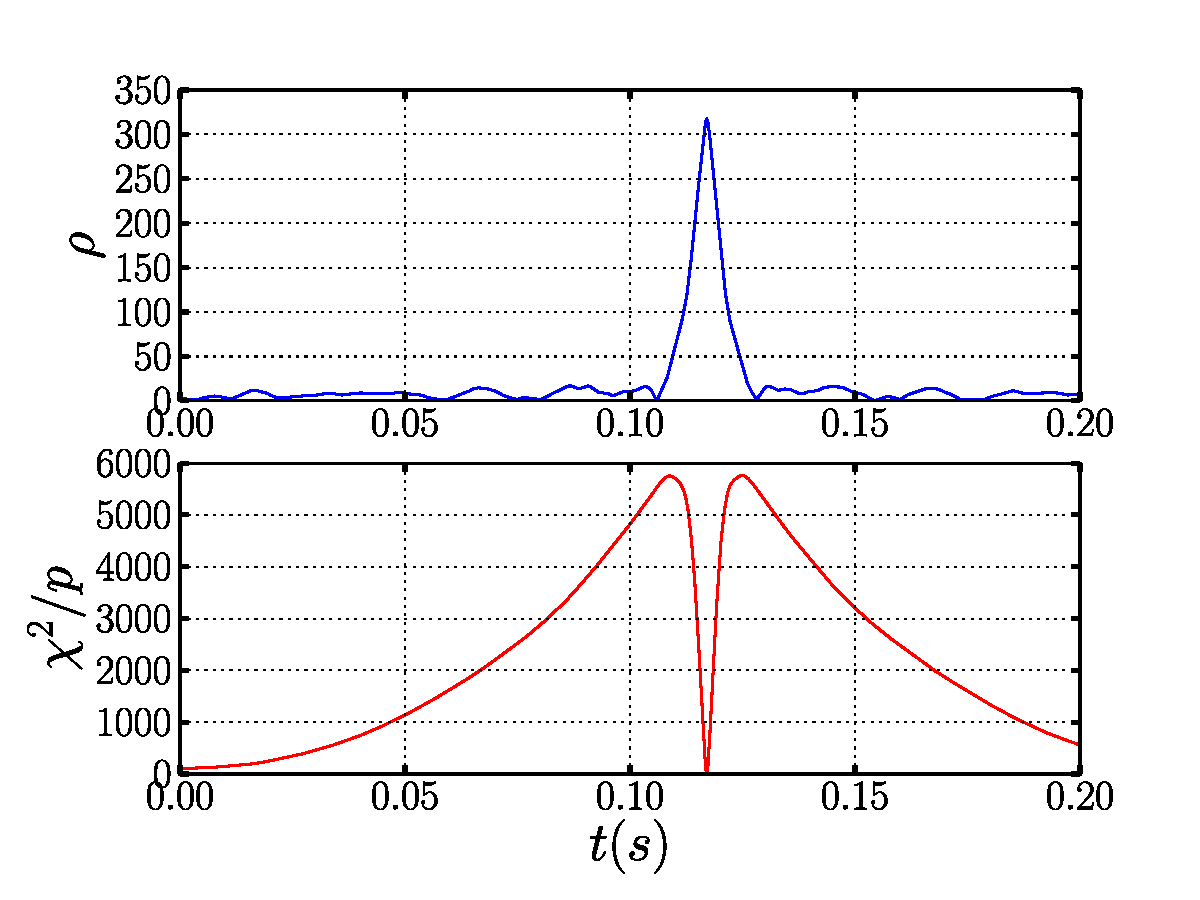
\includegraphics[width=0.75\linewidth]{images/2_searches/ihope_snr_timeseries.pdf}
    \caption{An SNR time series and $\chi^{2}$ time series for a simulated compact binary coalescence injected into S5~\cite{S5:2012} data with an SNR of $300$. Taken from~\cite{IHOPE:2012zx}.}
    \label{2:fig:ihope-snr-timeseries}
\end{figure}
%
The \( r^{2} \) test sets an upper threshold on the amount of time prior to the trigger as \(\chi^{2} \ge p r^{2}\), where \( p \) is the number of \(\chi^{2}\) sub-templates, with both the time window and \( r \) being determined empirically. The amount of time, $\Delta T$, threshold is a function of SNR
%
\begin{equation}
    \Delta T < 
    \begin{cases}
        2 \times 10^{-4} \, \text{s} \quad \text{for} \quad \rho < 12, \\
        \rho^{9/8} \times 7.5 \times 10^{3} \, \text{s} \quad \text{for} \quad \rho \ge 12.
    \end{cases}
\end{equation}
%
The amplitude consistency tests suppose the ratio of detector SNRs for true \gwadj signals should equal the ratio of detector sensitivities. We quantify detector sensitivity using the \textit{effective distance} $D_{eff, A}$, which is the distance at which an optimally located and oriented source would give the SNR observed by detector A. With an amplitude ratio threshold, $\mathfrak{A}^{*}$, we can construct another noise trigger discriminator
%
\begin{equation}
    \mathfrak{A} = 2 \frac{|D_{eff, A} - D_{eff, B}|}{D_{eff, A} + D_{eff, B}} \le \mathfrak{A}^{*}.
\end{equation}
%
The empirically determined threshold was found $\mathfrak{A}^{*} = 0.6$. We can also have the requirement that if a trigger is loud enough in detector A that we \textbf{should} have seen it in detector B, but we didn't, then we remove those triggers from the list. We note that historically this test was applied to the LIGO-Hanford-1 and LIGO-Hanford-2 detector combination which shared the same vacuum tubes at the LIGO-Hanford site, this test was not applied to another other combination of detector due to the different locations and orientations of the detectors producing any possible ratio of effective distances.

The final addition to this step is the inclusion of data quality vetoes where periods of increased glitch rate in the detectors have been removed from the analysis using data quality (DQ) flags~\cite{Slutsky:2010}. The detector's have many auxiliary channels which record environmental and instrumental information such as seismic noise monitors. These DQ flags are created automatically when periods of heightened detector noise is detected in these channel. The severity of the veto is divided into four categories where category 1 vetoes indicate data is entirely unusable and category 4 refers to good, science quality, data.

\subsubsection{Calculation of ranking statistic, false-alarm rates and search sensitivity}

The ranking statistic and false-alarm rates are calculated for each of these triggers as described in the previous section. The sensitivity of the search pipeline can be evaluated by injection a large number of simulated \gwadj signals into the data and recovering them with the search pipeline. The most realistic injections are hardware injections~\cite{Brown:2003, Biwer:2016} in which an actuator exerts a force on the end test mass to simulate the response of a real \gwadj signal. These injections are rarely performed because the data is now contaminated and cannot be used to search for real \gwadj signals. The injections used for large scale injection campaigns are software injections, in which the \gwadj signal is added to the data. These injections are added to add detectors with the correct time, phase and amplitude differences and are placed so as to probe the full population of potential \gwadj events. The injection campaigns are a very powerful tool that can reveal search pipeline sensitivity and we have used them extensively throughout this thesis to test the sensitivity increase of changes made to search pipelines.


%---% Detector Characterisation %---%
\chapter[Detector Characterisation]{\label{chapter:3-detchar}Detector Characterisation}\chapterquote{``This chapter needs a quote'' - Arthur Tolley}
%%%%%%%%%% %%%%%%%%%% %%%%%%%%%%

% Purpose of the chapter
In this thesis, we have made improvements to the search for \gws by improving the quality of the detector data and understanding the noise background of the detectors. 

% Section by section of chapter
This chapter is laid out as follows: we briefly repeat the state of the current \gwadj detector network in Section~\ref{3:sec:gw_detectors}, in Section~\ref{3:sec:detchar_calib} we define the research area of detector characterisation, the systematic sources of noise faced in the detectors are described in Section~\ref{3:sec:detector-analysis}, some common detector data noise transients in Section~\ref{3:sec:noise-transients} and finally, the detector characterisation tools most commonly used and referred to throughout this thesis in Section~\ref{3:sec:detchar-tools}.

\section{\label{3:sec:gw_detectors}\Gwadj detectors}

% To understand the importance of Detector Characterisation we must understand the detectors
\Gwadj astronomy in the present day is performed by ground-based detectors at different locations globally: the LIGO-Livingston and LIGO-Hanford detectors are located in the United States of America, the Virgo interferometer in Italy, and the KAGRA telescope in Japan. We will primarily reference the LIGO detectors in the United States of America when discussing the challenges faced in detector characterisation. 

As described in Chapter~\ref{chapter:1-gravitational-waves}, the LIGO detectors work on the principle of laser interferometry to detect \gwadj signals. The sensitivity~\cite{aLIGO_design_curve:2018} of \gwadj detectors is limited by fundamental sources of noise~\cite{PSD_var:2020} such as seismic noise~\cite{Glanzer:2023}, thermal noise~\cite{thermal_noise:2018} and quantum noise~\cite{quantum_noise:2003}. Additionally, we have non-Gaussian noise~\cite{Noise_Guide:2020}, which manifests as transient noise bursts in the data, which can contribute to false positives in \gwadj searches and the obscuring of real \gwadj signals~\cite{GW170817:2017, GW150914_noise:2016}.

\subsection{\label{3:sec:detector-analysis}Detector analysis}

% Noise analysis
%    Different sources of noise
%    Seismic, thermal, shot, radiation pressure
%    Noise Curve

Systematic sources of noise are the dominating limitation in the sensitivity of ground-based detectors. The sources of noise with the greatest contributions are
%
\begin{itemize}
    \item Seismic noise~\cite{Glanzer:2023}: the vibrations of the ground causes a coupled vibration motion in the mirrors of the interferometer. Higher frequency seismic noise ($1-10$Hz) is often caused by local ground movements typically anthropogenic in nature, or greater magnitude earthquakes~\cite{Nuttall:2018}. Lower frequency seismic noise ($<1$Hz) is caused by larger-scale geophysical processes such as ocean waves, tidal effects, or smaller local earthquakes~\cite{aLIGO:2015}. Seismic noise can be mitigated with advanced suspension systems to isolate mirrors and end-station components from the ground to prevent coupling to seismic motion~\cite{seismic_isolation:2015}.
    \item Thermal noise~\cite{thermal_noise:2018}: the thermal energy of interferometer components will cause them to vibrate. This noise can be reduced with new mirror materials with resonant frequencies outside the sensitive regions or with cryogenically cooled mirrors such as those used by KAGRA~\cite{KAGRA:2021}.
    \item Shot noise~\cite{quantum_noise:2003}: the distribution in the number of photons observed by the interferometer photodetector in any time interval is Poisson distributed, and the error in the photon count places limits on the sensitivity. The error is proportional to the square-root of the count ($\sigma \propto \sqrt{\lambda}$) therefore, the simplest way to reduce this error is to increase the laser power and increase the photon count in the time interval.
    \item Radiation pressure~\cite{quantum_noise:2003}: the pressure exerted by the photons hitting the end mirrors will decrease search sensitivity. To reduce this noise the laser power can be reduced; however, this will increase the shot noise.
\end{itemize}

It can be seen that the laser power must be calibrated to balance the impact of increasing the photon count which will decrease shot noise but simultaneously increase radiation pressure noise. A figure displaying these systematic noise sources and their limitations in the LIGO detector case can be seen in Figure~\ref{3:fig:aLIGO_noise}.
%
\begin{figure}
    \centering
    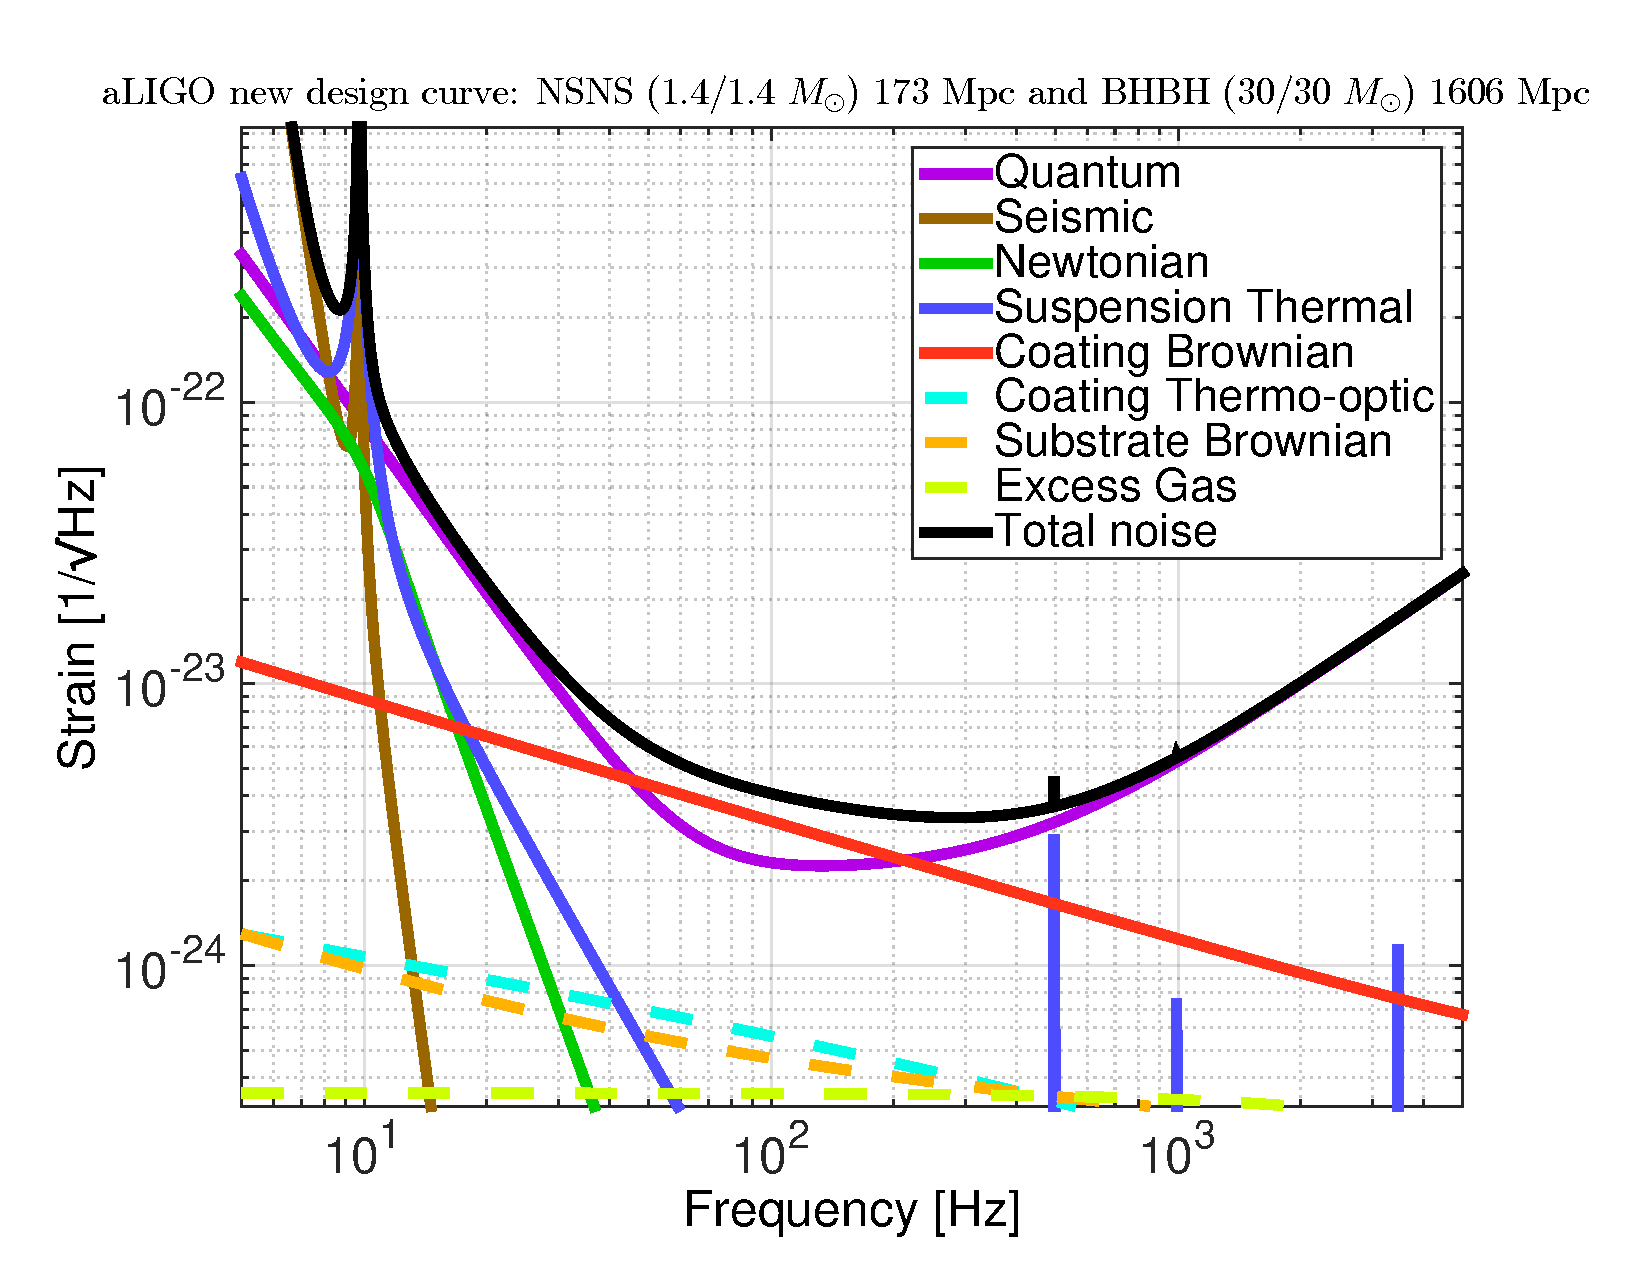
\includegraphics[width=0.75\linewidth]{images/3_detector_characterisation/aLIGO_newDesign.pdf}
    \caption{The Advanced LIGO~\cite{aLIGO:2015} strain sensitivity as a function of frequency (black solid line), accompanied by the systematic noise sources which limit the sensitivity of the detector. Taken from~\cite{aLIGO_design_curve:2018}.}
    \label{3:fig:aLIGO_noise}
\end{figure}
%

% Sensitivity Analysis
%    BNS Distance
%    Sensitivity Measurement
To monitor detector sensitivity, the binary neutron star inspiral range is calculated. This is the range at which a binary neutron star signal, with both components having a mass of $1.4$ M$_{\odot}$, will be detected given the characteristic noise (PSD) of the data. The PSD is calculated by taking an average of the detector noise in the previous minute~\cite{range_calculation:2003, ota:2023}. Figure~\ref{3:fig:bns_range} shows an example of the binary neutron star range for a day of LIGO-Hanford during the fourth observing run.
%
\begin{figure}
    \centering
    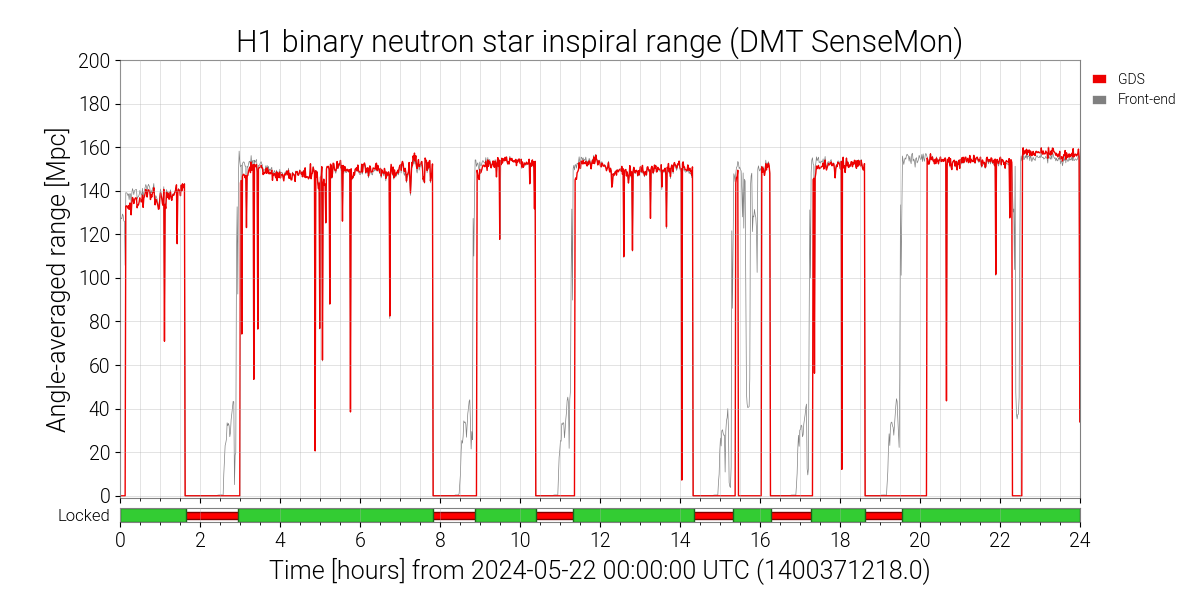
\includegraphics[width=1\linewidth]{images/3_detector_characterisation/may22_bns_range.png}
    \caption{The LIGO-Hanford binary neutron star inspiral range for the 22nd May 2024, created using GWSumm~\cite{gwsumm:2024} and taken from the LIGO Summary Pages-\href{https://summary.ligo.org/}{https://summary.ligo.org/}, please see \href{https://gwosc.org/detector_status/}{https://gwosc.org/detector\_status/} for the public summary pages.}
    \label{3:fig:bns_range}
\end{figure}
%

\subsection{\label{3:sec:noise-transients}Noise transients}

% Introduction to Noise Transients

Noise transients, commonly referred to as glitches, are short duration bursts of noise found in \gwadj data. The systematic sources of noise described in Section~\ref{3:sec:detector-analysis} limit the sensitivity of the detector to a certain frequency range, glitches appear within this sensitivity frequency range. The specific noise transients investigated by detector characterisation are non-Gaussian noise artefacts that have the ability to obscure~\cite{GW170817:2017} or mimic \gwadj signals~\cite{GWMimicking:2010}, producing false-alarms in our \gwadj search pipelines. Understanding these glitches is crucial for \gwadj detection; they have the potential to reduce the sensitivity and hinder the reliability of the detectors.
%
% GW170817 Obscured
%

% Characteristics of Noise Transients

There are at least $27$~\cite{gravityspy:2023, gravityspy:2024} different classes of glitch which all manifest with different durations (typically in the millisecond to second range), amplitudes, and glitch morphology. Glitches populate the whole sensitive frequency range of the detectors with some glitches being broadband, affecting up to the whole frequency bandwidth, to others being narrowband and affecting only specific frequency ranges. Glitches are commonly characterised and studied in 2-dimensional time-frequency representations of the one-dimensional strain time series that the detector outputs. The typical time-frequency representation used is the OmegaScan~\cite{qscan:2004} (referred to as `Omega scan' or `Q-scan') which is described later in this chapter.

% Common Sources of Noise Transients

Glitches originate from either environmental sources, instrumental sources, or a coupling of the two. As mentioned previously, seismic noise limits the sensitivity of the detectors below ${\sim}10 \, \text{Hz}$, but the coupling of seismic motion into interferometer components can cause one of the more common glitches---\scl. Other environmental noise sources are heavy winds, lightning, and human activity (traffic, construction, trains). A historical glitch identified at LIGO-Livingston was caused by an air conditioning compressor cycling, these glitches were seen by both a magnetometer and the \gwadj strain channel. Other instrumental glitches might be caused by mirror suspensions, electronics, control systems or laser fluctuations.

% Other examples of some common glitches

The most common glitches are: blips~\cite{blips:2019}, \scl~\cite{ArchEnemy:2023} and whistles~\cite{glitschen:2021}, Omega scans of these glitches can be seen in Figure~\ref{3:fig:glitches_subset}. The sources of these glitches have been studied. For example, whistles are caused by the beating of radio frequencies in the detector; however, some glitches come from unknown sources, such as blips. \Scl has been found from many sources in the detector and great effort has been made to reduce the presence of \scl in the data~\cite{reducing_scattering:2020} but as of the fourth observing run some \scl still remains.
%
\begin{figure}
    \centering
    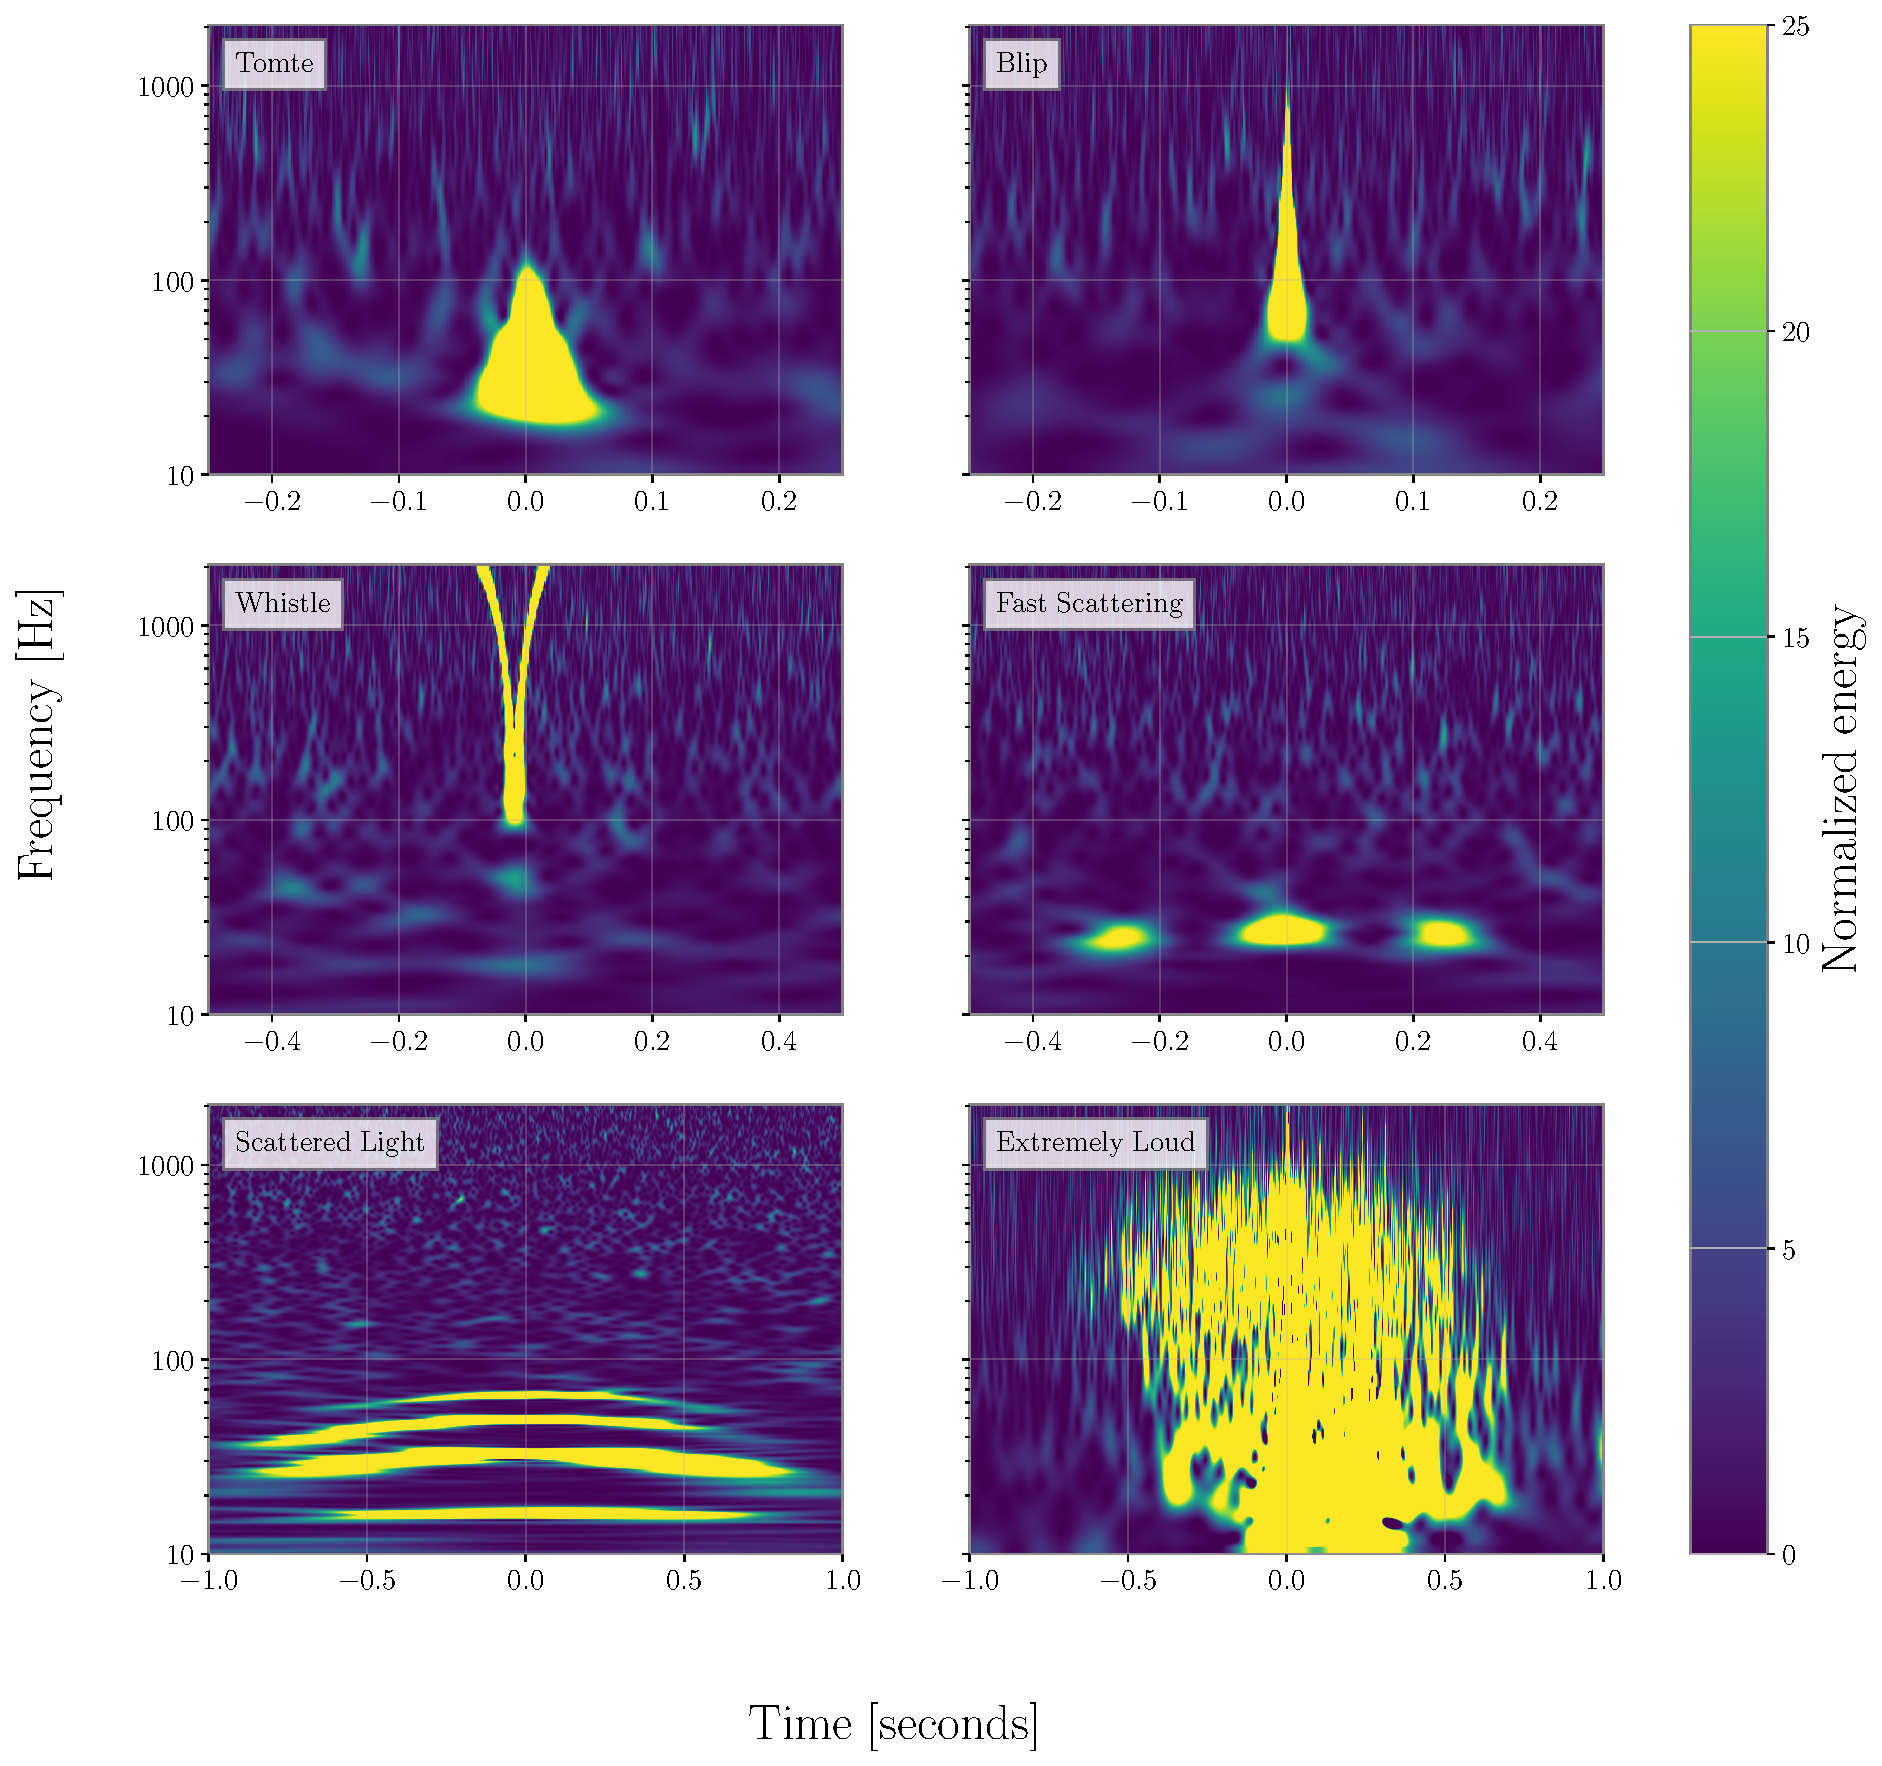
\includegraphics[width=1.0\linewidth]{images/3_detector_characterisation/glitches_subset.pdf}
    \caption{Six classes of glitch commonly found in LIGO detector data. Taken from~\cite{GlitchPlot:2024, gravityspy:2023}.}
    \label{3:fig:glitches_subset}
\end{figure}
%

% Detection and Characterisation of Noise Transients

A number of algorithms and tools have been developed to detect and characterise noise transients in \gwadj data~\cite{ArchEnemy:2023, reducing_scattering:2020, Glanzer:2023, gravityspy:2017, gravityspy:2021, gravityspy:2023, glitschen:2021,  BayesWave:2015, gwadaptive:2022, O3_subtraction:2022, Powell:2016, glitschen:2021}. The primary aim of these tools is the identification of glitches and analysis of properties of the glitches (amplitude, frequency, duration, waveform shape) to determine the source of the noise. Once the noise source has been identified improvements to the detector can be made to eliminate it. Other tools focus on modelling noise transients for the purpose of subtracting them from affected \gwadj data~\cite{ArchEnemy:2023, BayesWave:2015, glitschen:2021, antiglitch:2023}.
%
% GravitySpy figure of a bunch of glitch classes
%

% Auxiliary Channels

Another tool used in the identification and classification of glitches is the thousands of auxiliary channels alongside the main strain channel~\cite{iDQ:2020}, which monitor the many subsystems of the detector and can be used to find noise correlations between the different parts of the instrument~\cite{DQ_vetoes:2017}. The auxiliary channels which are not sensitive to \gws are very useful in identifying any correlations between noise in the gravitational strain channel and noise also seen in another channel which cannot observe \gws, an example of this is the magnetometer recording the same glitch as seen in the \gwadj strain channel when the air conditioning compressor was cycling at LIGO-Livingston~\cite{Nuttall:2018}.

\section{\label{3:sec:detchar_calib}Detector characterisation and calibration}

Detector characterisation is a field of study which assess and improves the performance of \gwadj detectors to ensure accurate and reliable detection of \gws. \Gwadj detector calibration determines how the response of the detector translates to astrophysical signals, ensuring accuracy in extracted astrophysical information. Detector characterisation is responsible for identifying and mitigating the many sources of noise that can obscure or mimic real signals. The optimisation of detector sensitivity is also studied, whereby different designs and components can be fine-tuned to increase sensitivity. Another responsibility of detector characterisation is the monitoring of detector performance in real-time to assess sensitivity changes.

Overall, effective detector characterisation ensures that \gwadj observatories can operate at maximum potential and provide accurate and reliable observations of \gws. The \gwadj detector organisations have dedicated working groups for detector characterisation and calibration~\cite{O2O3_DetChar:2021, VirgoDetChar:2023}. In this thesis, chapter~\ref{chapter:4-archenemy} is a direct contribution to the field of detector characterisation with a contribution to the LIGO detector characterisation working group.

The detector characterisation group has the important task of verifying data quality when a \gwadj signal is detected by live detection pipelines, giving the confirmation that the \gwadj signal isn't a false alarm potentially caused by noise transients or poor data quality immediately surrounding the \gwadj signal.

\subsection{\label{3:sec:detchar-tools}Detector characterisation tools}

\paragraph{Omega scans}

are two-dimensional time-frequency representations of \gwadj data used very commonly to display \gwadj data in a human interpretable fashion, which contains more information than a simple spectrogram and can reveal time-frequency relationships that are virtually impossible for humans to see in the time series. Example Omega scans can be seen in Figure~\ref{3:fig:glitches_subset} for a number of glitches.

Detector characterisation uses Omega scans to highlight glitches which can have sharp and localised features in the time-frequency plane. Omega scans calculate the amplitude of strain power at each pixel using the \textit{Q-transform}~\cite{qscan:2004}, where for each point in time and frequency a number of wavelets are created with a varying \textit{quality factor} ($Q$). $Q$ is calculated using
%
\begin{equation}
    Q = \frac{f_{c}}{\sigma_{f}},
\end{equation}
%
where $f_{c}$ is the central frequency and $\sigma_{f}$ is the bandwidth of a wavelet. The bandwidth has a uncertainty relation with the duration, $\sigma_{t}$ of the wavelet
%
\begin{equation}
    \sigma_{t} \sigma_{f} \ge \frac{1}{4\pi},
\end{equation}
%
and so a wider frequency bandwidth will lead to a shorter duration for the wavelet, balanced by the Q-factor. The Q-transform of all these wavelets with the \gwadj strain is taken
%
\begin{equation}
    H(\tau, f, Q) = \int^{\infty}_{-\infty} h(t) w(t - \tau, f, Q) dt,
\end{equation}
%
and the Omega scan algorithm will select the wavelet which produces the greatest amount of power ($|H(\tau, f, Q)|^{2}$) per pixel. As an example, a short-duration glitch (like a blip) would be better tiled with multiple low-frequency bandwidth, high-Q tiles which will resolve the glitch in greater definition than a low-Q tile which captures the whole glitch in one tile.

\paragraph{GravitySpy}

is a citizen science machine learning tool for classifying glitches found in \gwadj data~\cite{gravityspy:2017}. GravitySpy has been trained by volunteers at the project website:~\href{https://www.zooniverse.org/projects/zooniverse/gravity-spy}{https://www.zooniverse.org/projects/zooniverse/gravity-spy}, hosted on the Zooniverse~\cite{zooniverse}.

GravitySpy has uploaded more than $1.4$ million of Omega scans of \gwadj data which have been found to contain bursts of power which could be caused by glitches. The Omega scans are published on the GravitySpy project and volunteers are given these images and the option for which glitch they think is contained within the image. Once these images have been classified the machine learning algorithm is trained and it can go further to classify the images without the need of volunteers~\cite{gravityspy:2021}.

GravitySpy has been run on data from the second and third observing runs, where it was able to classify 24 different glitch categories. The downsides of GravitySpy are the constantly changing noise background of the \gwadj detectors and the new glitch types emerging which need to be trained on with volunteering again~\cite{gravityspy:2023}.

\paragraph{Data Quality Vetoes} are a flag applied to periods of data which contain potential data quality issues~\cite{DQ_vetoes:2017}. These periods of data are identified using the ${\sim}200,000$ auxiliary channels~\cite{DQ_vetoes:2017}, an example is a significantly elevated transient noise rate in the strain channel five days prior to GW150914~\cite{GW150914:2016} which was traced back to the $45 \, \text{MHz}$ electro-optic modulator driver system used to generate optical cavity control feedback signals~\cite{aLIGO:2015}. The noise caused by this channel was given a category 1 veto data quality flag and removed 2.62\% of the total coincident time from the analysis period. While there is a significant reduction in the number of high SNR triggers that would've been found during these times, these flags fallen out of favour in the fourth observing run due to removing large amounts of data.


%---% ArchEnemy %---%
\chapter[ArchEnemy]{\label{chapter:4-archenemy}ArchEnemy}
\chapterquote{``This chapter needs a quote'' - Arthur Tolley}
I am first author on a peer-reviewer and published work carrying the name \textit{"ArchEnemy: Removing scattered-light glitches from gravitational wave data"}, within the Institute of Physics journal Classical and Quantum Gravity~\cite{ArchEnemy:2023}.
\section{\label{4:sec:ArchEnemy-intro}Introduction}

The Laser Interferometer Gravitational-Wave Observatory (LIGO)~\cite{aLIGO:2015} and Virgo~\cite{aVirgo:2015} collaborations made the first observation of \gws{} in September 2015~\cite{GW150914:2016}. The detection established the field of \gw{} astronomy and a global network of \gw{} detectors, now joined by KAGRA~\cite{KAGRA:2021}, has allowed for the detection of approximately 100 \gw{} events~\cite{gwtc1:2019, gwtc2:2021, gwtc21:2024, gwtc3:2023, 1OGC:2018, 2OGC:2020, 3OGC:2021}.

The detection of \gws{} is made possible by both the sensitivity of the detectors and the search pipelines~\cite{PyCBC:2016, GstLAL:2020, SPIIR:2020, MBTA:2021, cWB:2020} which analyse raw strain data from the output of the detectors and identify observed \gw{} signals. One of the problems that these search pipelines must deal with is the fact the data contains both non-stationary noise and short duration `glitches'~\cite{Noise_Guide:2020, O2O3_DetChar:2021, VirgoDetChar:2023} where noise power increases rapidly. Glitches are caused by instrument behaviour or interactions between the instrument and the environment~\cite{GW150914_noise:2016, Glanzer:2023} and glitches reduce the sensitivity of the detectors~\cite{O3_sensitivity:2020}, can potentially obscure candidate \gw{} events~\cite{gwtc2:2021} and can even mimic \gw{} events~\cite{GWMimicking:2010, PyCBC_singles:2022}.

Different classes of glitches have been characterised using tools such as Gravity Spy~\cite{gravityspy:2017, gravityspy:2023}. Of the 325,101 glitches classified by Gravity Spy in the third observing run of Advanced LIGO~\cite{gravityspy:2021} with a confidence of $90\%$ or higher, 120,733 ($32.1\%$) were classified as ``Scattered Light''. \Scl{} glitches occur in the 10-120Hz frequency band~\cite{reducing_scattering:2020} which coincides with the frequency band where we observe the inspiral and merger signatures of compact binary coalescences. \Scl{} glitches are characterised by an arch-like pattern in a time-frequency spectrogram of the detector output, as seen in figure~\ref{4:fig:scattered_light}. 
%
\begin{figure}
  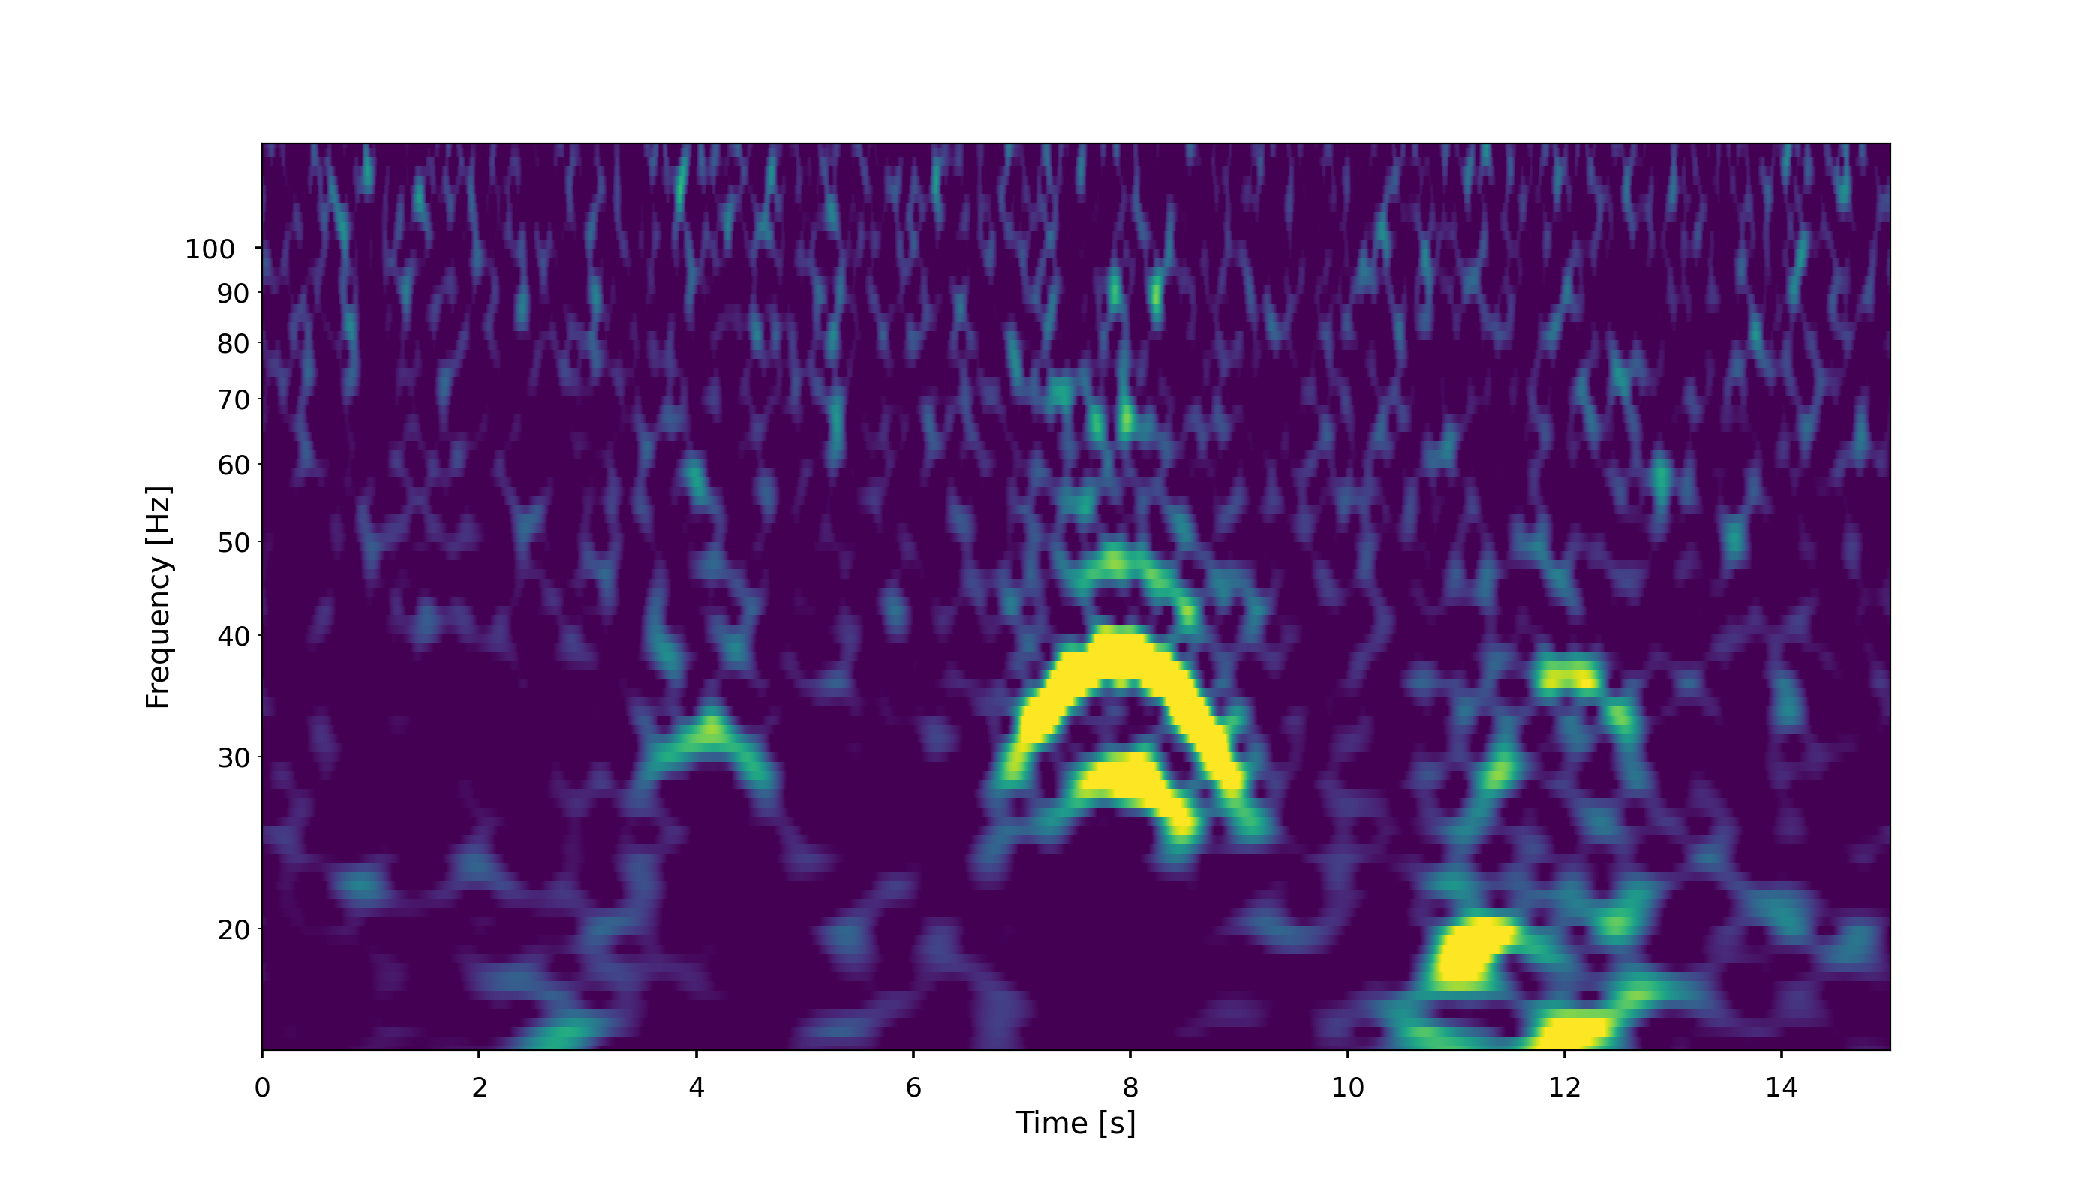
\includegraphics[width=\textwidth]{images/4_archenemy/Section1/single_stack.pdf}
  \caption{An Omega scan \cite{gwdetchar_tools:2021} of \gw{} data containing an example of a \scl{} glitch. \Scl{} glitches are characterised by a symmetric arch-like pattern. Multiple \scl{} glitches can be seen at the 4, 8 \& 12 second marks as well as multiple harmonic glitches at 8 seconds.}
  \label{4:fig:scattered_light}
\end{figure}
%
\Scl{} glitches occur when laser light in the interferometer is scattered from the main optical path by components within the detector. The motion of these components is coupled to seismic motion inducing a phase shift on the light being scattered as the surface moves back and forth. This \scl{} then recombines with the main laser, producing \scl{} glitches in the data. The surfaces from which \scl{} glitches originate have been objects on optical benches such as lenses, mirrors and photo-detectors~\cite{TAccadia:2010}.

\Scl{} glitches have been a significant problem when observing compact binary mergers. As an example, GW190701\_203306 was coincident with a \scl{} glitch, as shown in figure \ref{4:fig:obscured_detection}~\cite{gwtc2:2021}, requiring subtraction from the data before the event could be properly characterised~\cite{O3_subtraction:2022}. A further 7 candidate events were found to be in coincidence with \scl{} glitches in the third observing run~\cite{gwtc3:2023}. For this reason, it is important to reduce the effect of \scl{} glitches in the detectors and \gw{} search pipelines. \Scl{} glitches occur as single or multiple glitches and can appear rapidly in time and simultaneously in frequency (see figure \ref{4:fig:consec_scattered_light}), which we refer to as harmonic glitches.

\begin{figure}
  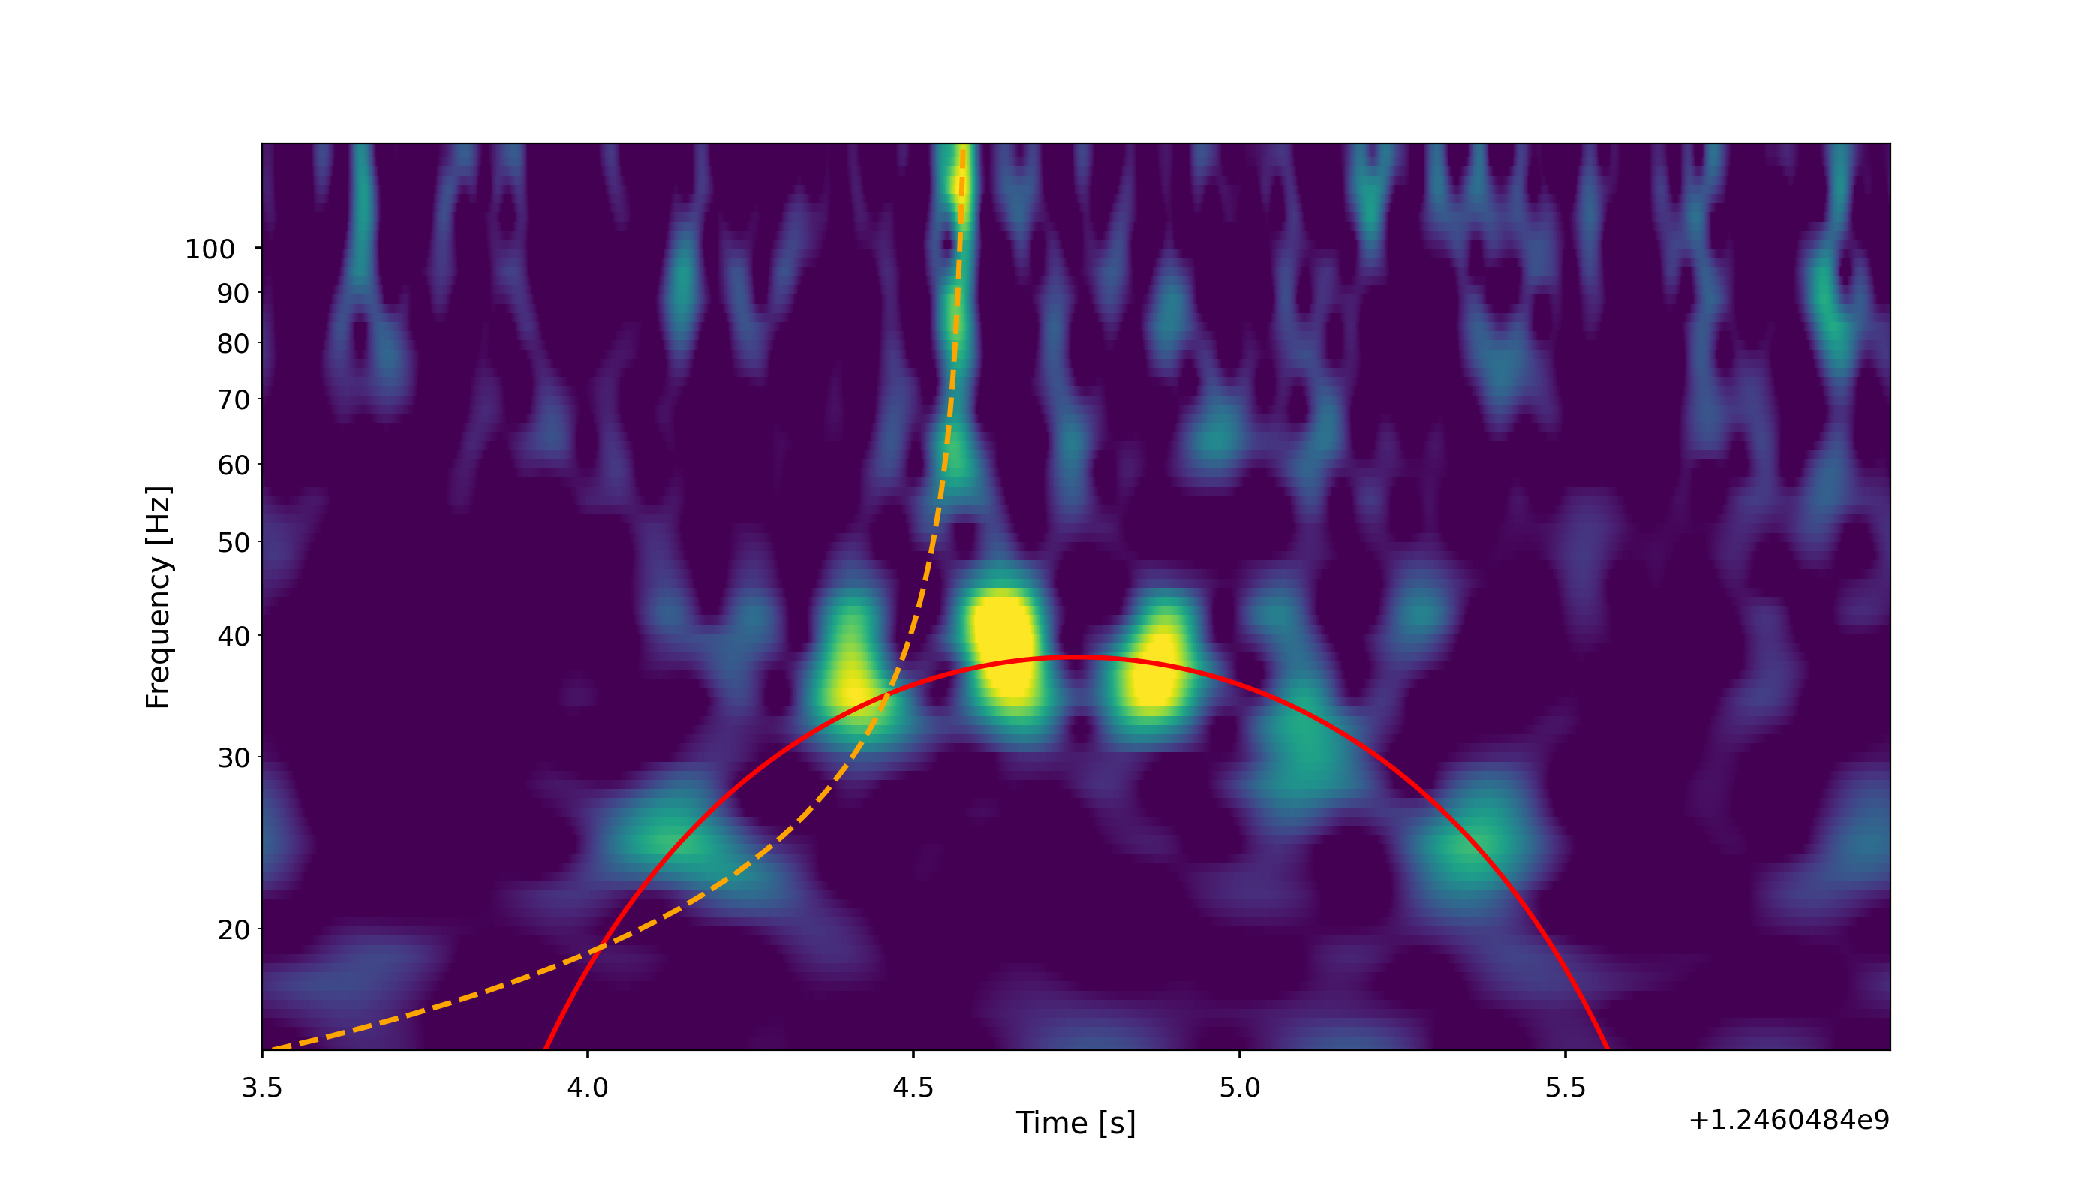
\includegraphics[width=\textwidth]{images/4_archenemy/Section1/GW190701_203306_overlay.pdf}
  \caption{GW190701\_203306, a \gw{} event coincident with a \scl{} glitch in the data from the LIGO Livingston observatory. The orange dashed track shows the inferred time-frequency evolution of a \gw{} event produced by a compact binary merger, the red solid line is an overlaid track of the approximate location of the coincident fast scattering glitches.}
  \label{4:fig:obscured_detection}
\end{figure}

\begin{figure}
  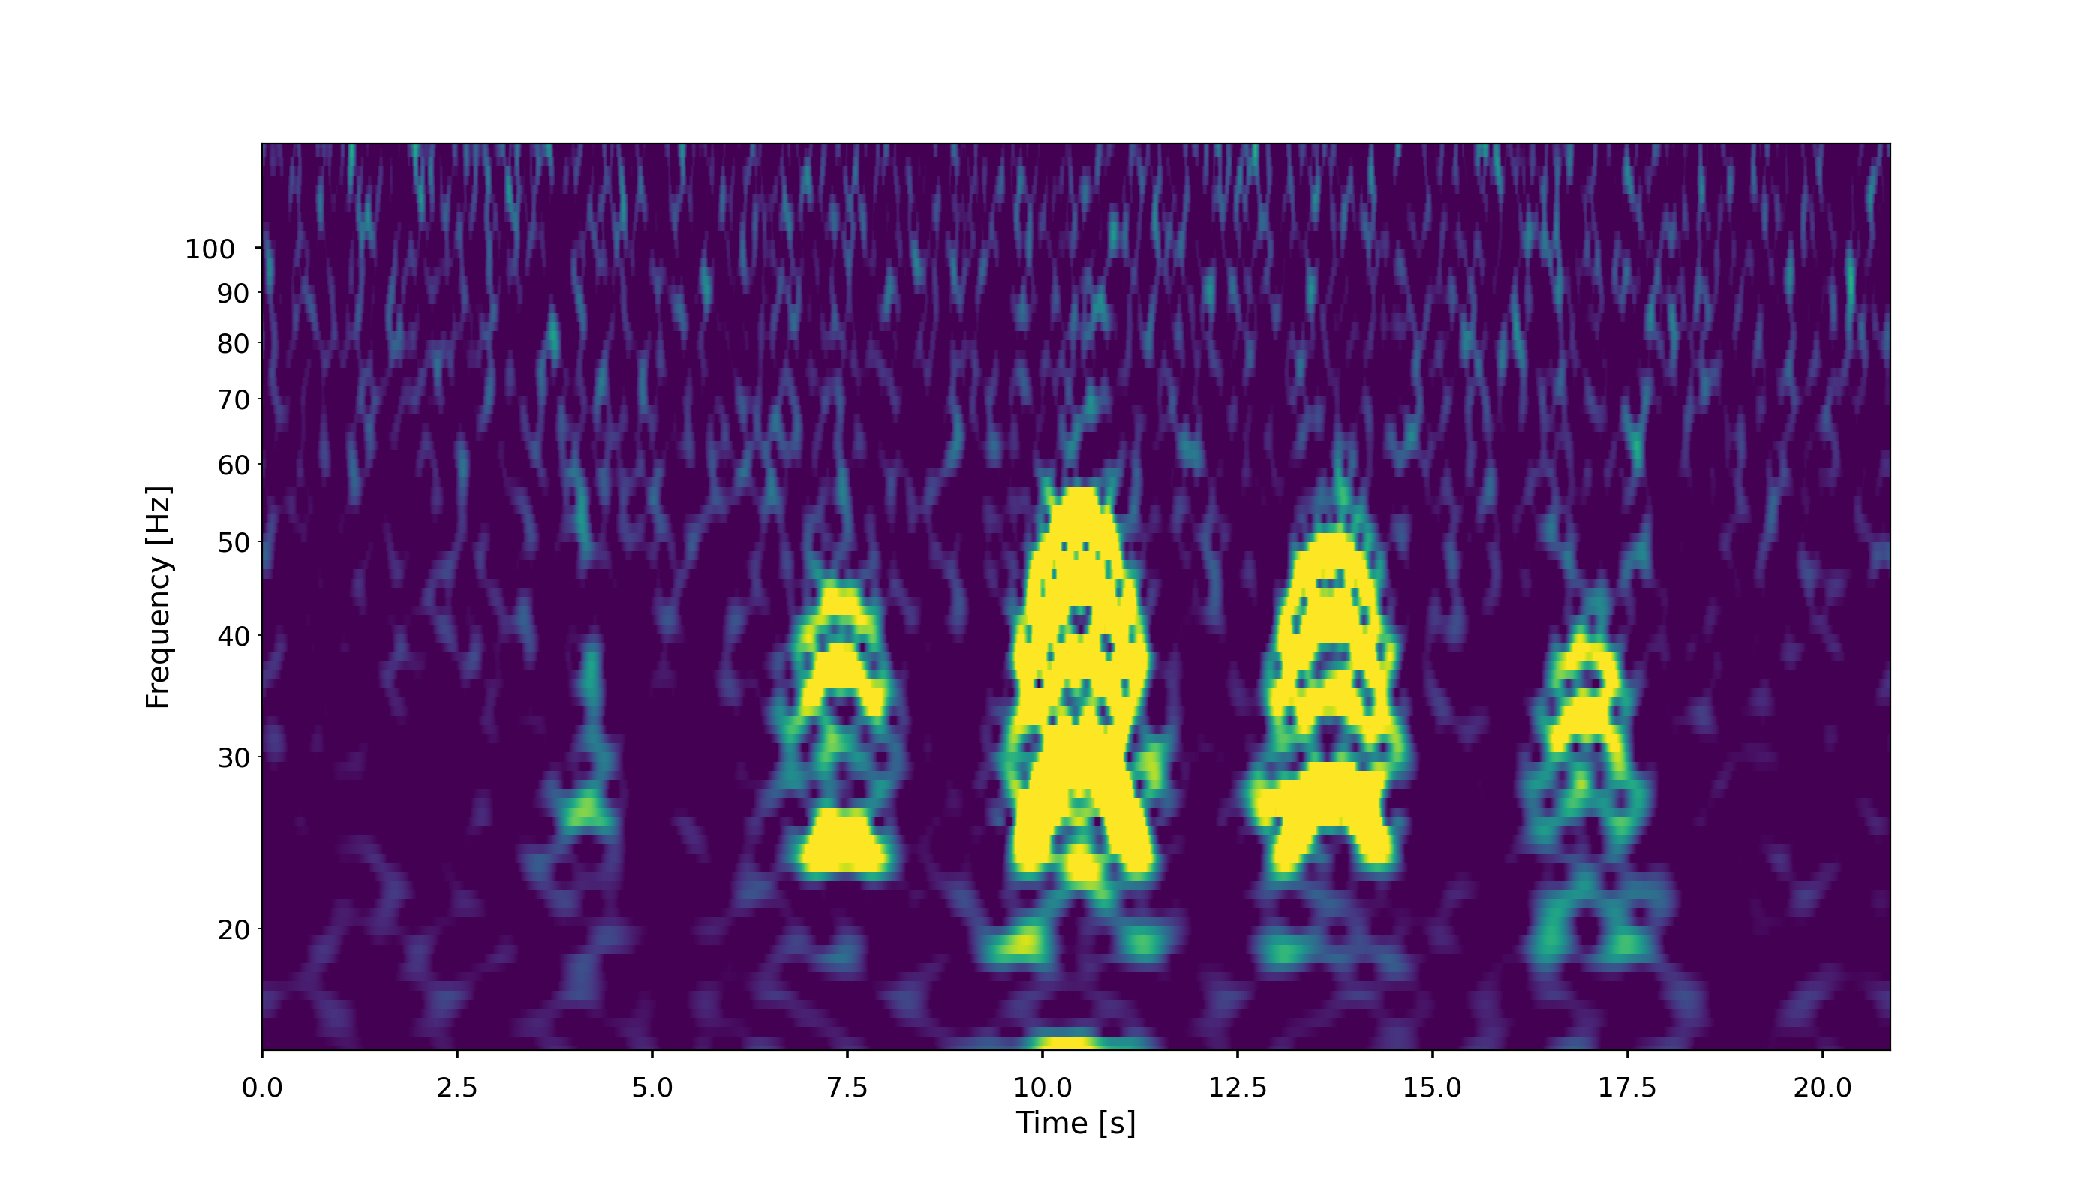
\includegraphics[width=\textwidth]{images/4_archenemy/Section1/multiple_harmonics.pdf}
  \caption{An Omega scan \cite{gwdetchar_tools:2021} of \gw{} data containing multiple examples of \scl{} glitches. Here we see multiple \scl{} glitches repeating periodically in a $20$ second period of time. Harmonic \scl{} glitches are also seen in multiple stacks, the harmonic glitches share \emph{time period} values and the \emph{glitch frequency} values are $n-$multiples of the lowest frequency harmonic within the stack.}
  \label{4:fig:consec_scattered_light}
\end{figure}

The most obvious way to remove the impact of glitches is removing the mechanisms which produce the glitches in the observatories. This has been investigated in previous works~\cite{reducing_scattering:2020, TAccadia:2010, Nuttall:2018, gwadaptive:2022, HilbertHuang:2017, tvf-EMD:2020, Scattering_Monitoring:2022, Was_Subtract:2021}, which focus on identifying the surfaces in which light is being scattered from and then mitigating the scattering by reducing the reflectivity of the surface, seismically isolating it or relocating it. 

An alternative method for reducing \scl{} glitches, known as ``RC tracking'', was implemented in the Advanced LIGO observatories in January 2020~\cite{reducing_scattering:2020}. The Advanced LIGO detectors employ a quadruple pendulum suspension for the test masses where two chains suspend four masses in this suspension system, one for the test mass optic and the other for the reaction mass. The reaction mass is used to impose a force upon the test mass and a significant source of \scl{} glitches was the large relative motion between the test mass chain and the reaction chain. To mitigate this effect, the relative motion between the end test mass and the reaction mass needed to be reduced. This was achieved by ensuring the two chains are moving together by applying force to the top stage of the quadruple suspension system in Advanced LIGO. The implementation of RC tracking represented a decrease from $0.01 s^{-1}$ to $0.0001 s^{-1}$ and $0.0072 s^{-1}$ to $0.0012 s^{-1}$ in the number of \scl{} glitches detected by Gravity Spy for LIGO-Hanford and LIGO-Livingston respectively.

While methods for preventing \scl{} glitches have been developed and have shown success, they have not been able to remove the problem of \scl{} glitches from the data. Additionally, as the detectors continue to be upgraded and increase in sensitivity, new sources of \scl{} glitches will continue to appear. Identifying these new sources and mitigating their effects can take many months, during which time the detectors are taking in data which might be affected by the presence of \scl{} glitches. Therefore, it is not realistic to believe that analyses will be able to regularly run on data that does not contain \scl{} glitches and this motivates us to develop a technique for mitigating the impact of these glitches when trying to identify compact binary mergers in \gw{} data.

In this work we present a new method for identifying and removing \scl{} glitches from \gw{} data in advance of running searches to identify compact binary mergers.
We first introduce a method for identifying when \scl{} glitches are present in detector data, through the creation of a new modelled search for \scl{} glitches, similar to how we search for \gws{} using matched filtering. We can model \scl{} glitches, generate a suitable set of glitch waveforms and perform a matched filter search on detector data. We then subtract identified glitches from the data to increase detector sensitivity. The detector data isn't Gaussian and stationary so the matched filter does have the potential to identify non-\scl{} glitches, and potentially even \gw{} signals, as \scl{} glitches. To prevent this we also demonstrate a new \scl{} $\chi^{2}$ test, which can distinguish between \scl{} glitches, and other glitches---and \gw{} signals---in the data.

We begin by reviewing previous research and describing the formulation of the waveform model used for characterizing \scl{} glitches in section \ref{4:sec:sc_li}. In section \ref{4:sec:search_techniques} we introduce the various techniques used in the search to identify \scl{} glitches in \gw{} data and the results of the \scl{} glitch search. In section \ref{4:sec:results} we describe the results of a ``glitch-subtracted'' \gw{} search and any increases in sensitivity. We conclude in section \ref{4:sec:conclusion} and discuss the implementation of this method in future observing runs.

\section{\label{4:sec:sc_li}\Scl{}}

To identify \scl{} glitches in \gw{} data requires an accurate model of \scl{} glitches. This section details the derivation of the model we will use for generating our \scl{} glitch filter waveforms, along with its parameterisation.

\subsection{Modelling \scl{} glitches - a review}

Our model for \scl{} glitches draws heavily from~\cite{TAccadia:2010}, and we briefly review the main details of the model presented there. In~\cite{TAccadia:2010}, the authors construct a model to accurately predict the increase in noise due to \scl{} during periods of increased micro-seismic activity. The model in~\cite{TAccadia:2010} is constructed from parameters related to physically measurable properties of the detector such as the mirror transmission factor, $T$, the finesse of the Fabry–Pérot cavity, $F$, or the wavelength of the light, $\lambda$.

They define the amplitude of the additional beam produced by light scattering off of a surface as
%
\begin{equation}
    A_{sc} = A_{0} T \sqrt{\frac{2 F}{\pi}} \sqrt{f_{sc}} e^{i \phi_{sc}}\,,
    \label{4:eqn:accadia_amplitude}
\end{equation}

%
where $A_{0}$ is the amplitude of the light resonating in a Fabry–Pérot cavity, $f_{sc}$ is the fraction of the optical power scattered back into the main beam and $\phi_{sc}$ is the phase angle modulated by the displacement of the scattering optics, defined as
%
\begin{equation}
    \phi_{sc}(t) = \frac{4 \pi}{\lambda} ( x_{0} + \delta x_{opt}(t) ),
    \label{4:eqn:accadia_phase_noise}
\end{equation}
%
where $\delta x_{opt}$ is the displacement of the scattering surface and $x_0$ is the static optical path.

The total amplitude of the beam inside the arm is given by $A_{tot} = A_{0} + A_{sc}$, with a phase angle equal to the phase noise introduced by the \scl{} $\delta \Phi = \frac{A_{sc}}{A_{0}} \cdot \sin \phi_{sc}$. The noise introduced by the \scl{}, $h_{sc}$, can be approximated through the relationship $\sin(\Phi_0+ \delta\Phi) \approx \cos(\Phi_0) \times \sin(\delta \Phi)$ for small $\delta\Phi$, and can be expressed as
%
\begin{equation}
    h_{sc}(t) = G \cdot \sin \left(\frac{4 \pi}{\lambda} (x_{0} + \delta x_{sc}(t) ) \right),
    \label{4:eqn:accadia_strain}
\end{equation}
%
where $G$ is the \emph{coupling factor}, defined as $K \cdot \sqrt{f_{sc}}$ where
%
\begin{equation}
K = \frac{\lambda}{4 \pi} \frac{T}{\sqrt{2 F \pi}}.
\end{equation}
%

The displacement of the scatterer when presenting with oscillatory motion is then given as
%
\begin{equation}
    \delta x_{sc} (t) \simeq A_{m} \sin(2 \pi f_{m} t),
    \label{4:eqn:accadia_oscillatory}
\end{equation}
%
where $f_{m}$ is the frequency-modulated signal with modulation index $m = A_{m} \frac{4 \pi}{\lambda}$ and where $A_{m}$ is the amplitude of the $n$th harmonic. Finally, equation~\ref{4:eqn:accadia_strain} can be simplified when considering only small bench motion, according to
%
\begin{equation}
    h_{sc}(t) = G \cdot \cos\phi_{0} \cdot \frac{4 \pi}{\lambda} \cdot \delta x_{sc}(t) \;.
    \label{4:eqn:accadia_strain_linearised}
\end{equation}

\subsection{Model}

The model introduced in~\cite{TAccadia:2010} for the \gw{} strain noise introduced by \scl{} uses a lot of knowledge about the detector state. The model used in this work will be more phenomenological in the parameterisation, allowing us to rely only on the characteristics of the glitches in the strain data and not knowledge of the detector configuration, especially in cases where this detector information might not be known. Each \scl{} glitch, as viewed in a spectrogram (see figure \ref{4:fig:scattered_light}), has two easily identifiable features: the maximum frequency reached, \emph{glitch frequency} ($f_{gl}$); and the period of time the glitch exists in detector data, \emph{time period} ($T$).  In addition we can fully describe an artifact by defining an \emph{amplitude} ($A$), \emph{phase} ($\psi$) and \emph{center time} of the glitch ($t_0$).

To formulate a model of \scl{} glitches in terms of these parameters, we simplify equation \ref{4:eqn:accadia_strain_linearised}, treating the strain noise caused by \scl{} as the sinusoidal function
%
\begin{equation}
  h_{sc}(t) \propto \sin(\phi_{noise}(t)).
  \label{4:eqn:h_sc_initial}
\end{equation}
%
Here the induced phase noise ($\phi_{noise}$) is equal to 
%
\begin{equation}
    \phi_{noise}(t) = 2 \pi f_{rep} t,
     \label{4:eqn:phi_noise}
\end{equation}
%
and $f_{rep}$ is the frequency of repetition of the sinusoid and is directly related to the \emph{time period}, $T$,
%
\begin{equation}
  f_{rep} = \frac{1}{2 T}.
  \label{4:eqn:f_rep}
\end{equation}
%
The \emph{time period} of a \scl{} glitch only corresponds to half of a sinusoidal wave hence the multiplier of 2 on the denominator of equation \ref{4:eqn:f_rep}.

\Scl{} glitches are caused by the physical increase in the distance travelled by the light as a consequence of being reflected off of a surface. The light returning to the beam splitter from one arm will have travelled a different path length compared to the other arm and this path difference will act as a phase difference between the two arms causing non-destructive interference. The path difference and phase difference can be related with
%
\begin{equation}
  \Delta \phi_{scattering}(t) = 2 \cdot \frac{2 \pi}{\lambda} \Delta x(t),
  \label{4:eqn:delta_phi_scat}
\end{equation}
%
where $\Delta x(t)$ indicates the change in the path taken by the light over time. An additional multiplier of 2 indicates our path difference is occurring twice, once when the light approaches the surface and again when leaving.

We assume the scattering surfaces are oscillatory in motion and apply the same simplification made in equation \ref{4:eqn:accadia_oscillatory}, with an initial position $\Delta x = 0$ to a maximum displacement of $x_{0}$. This produces an equation for the path difference of the light,
%
\begin{equation}
  \Delta x(t) = x_{0} \sin(2 \pi f_{rep} t).
  \label{4:eqn:delta_x_t}
\end{equation}
%
We substitute equation \ref{4:eqn:delta_x_t} into equation \ref{4:eqn:delta_phi_scat} and produce an equation for the phase noise induced by \scl{}
%
\begin{equation}
  \phi_{scattering}(t) = \frac{4 \pi}{\lambda} x_{0} \sin(2 \pi f_{rep} t) \;,
  \label{4:eqn:phi_sc}
\end{equation}
%
this equation for the phase noise induced by \scl{}, $\phi_{scattering}(t)$, and the equations for the generic phase noise, $\phi_{noise}(t)$ (equation \ref{4:eqn:phi_noise}), can now be used to create an equation for the strain noise caused by \scl{}.

We take the derivatives of equations \ref{4:eqn:phi_noise} $\&$ \ref{4:eqn:phi_sc} with respect to time:
%
\begin{equation}
  \phi_{noise} ^\prime (t) = 2 \pi F_{inst} (t),
\end{equation}
%
\begin{equation}
  \phi_{scattering} ^\prime (t) = \frac{4 \pi}{\lambda} x_{0} 2 \pi f_{rep} \cos(2 \pi f_{rep} t) \;,
\end{equation}
%
where $F_{inst}$ is the instantaneous frequency at a specific time. We generate \scl{} glitches from $\frac{-T}{2}$ to $\frac{T}{2}$ to ensure their maximum frequency occurs at $t = 0$. We define this maximum frequency as the \emph{glitch frequency}.

We equate the two derivatives and set $t = 0$, this replaces $F_{inst}(t)$ with $f_{gl}$ and $\cos(2\pi f_{rep} t)$ with $1$, then re-arrange to find the maximum displacement of the scattering surface, $x_{0}$, as
%
\begin{equation}
  x_{0} = \frac{f_{gl}}{f_{rep}} \frac{\lambda}{4 \pi}.
  \label{4:eqn:x0}
\end{equation}
%
Substituting equation \ref{4:eqn:x0} into equation \ref{4:eqn:phi_sc} gives us an expression for the \scl{} phase noise,
%
\begin{equation}
  \phi_{scattering}(t) = \frac{f_{gl}}{f_{rep}} \sin(2 \pi f_{rep} t),
  \label{4:eqn:phi_sc2}
\end{equation}
%
and substituting equation \ref{4:eqn:phi_sc2} as our $\phi_{noise}$ in equation \ref{4:eqn:h_sc_initial} we arrive at our model of \scl{} glitches,
%
\begin{equation}
  h_{sc}(t) = A \sin\left(\frac{f_{gl}}{f_{rep}} \sin(2 \pi f_{rep} t) + \psi\right),
  \label{4:eqn:model}
\end{equation}
%
where $A$ and $\psi$ are amplitude and phase parameters to be maximised over.

In~\cite{Was_Subtract:2021} they provide another term to describe \scl{} glitches which uses the instantaneous frequency as a function of time, allowing the identification of the correct amplitude at all frequencies. This term is due to radiation pressure coupling and is thought to be dominant at low frequencies. The relationship between our amplitude and the new amplitude depends on the power in the arm cavities and the signal recycling mirror reflectivity which we do not consider in our model and so disregard this extra term.

\subsection{Harmonics}

As described in~\cite{TAccadia:2010}, harmonic glitches appear at the same time with different \emph{glitch frequencies}. A harmonic glitch is a glitch with a \emph{glitch frequency} that is a positive integer multiple of the glitch frequency of the glitch in the stack with the lowest glitch frequency value. This lowest frequency glitch has the potential to appear below $15$Hz and will be masked by other sources of noise and therefore cannot be seen. An example of harmonics can be seen in figure \ref{4:fig:consec_scattered_light}.

%Section
\section{\label{4:sec:search_techniques}Identifying \scl{} glitches in \gw{} strain data}

Equipped with our model for \scl{} glitches from the previous section, we now discuss how we identify and parameterize \scl{} glitches in a stretch of \gw{} data before we apply this to searches for compact binary mergers in the next section. 

\subsection{\label{4:subsec:MF}Matched filtering}

Given our model of \scl{} glitches, we can consider a realisation with specific values of the parameters discussed above. To identify glitches with these values of the parameterisation, we follow the same technique as that commonly used to identify compact binary mergers and apply matched filtering. The matched filter is defined as~\cite{FINDCHIRP:2012}
%
\begin{equation}
  \rho(t) = \frac{(h | s)}{\sqrt{(h | h)}} \equiv (\hat{h} | s).
  \label{4:eqn:mf_1}
\end{equation}
%
Here $h$ is the model template, $s$ the \gw{} data we are searching and we use the noise-weighted inner product defined between two time series $a(t)$ and $b(t)$ as
%
\begin{equation}
  (a | b) = 4 Re \int^{\infty}_{0} \frac{\tilde{a}(f) \tilde{b}^*(f)}{S_n(f)} 
  %e^{-2 \pi i f t} 
  df.
  \label{4:eqn:inner_product}
\end{equation}
%
The tilde on $\tilde{a}$ and $\tilde{b}$ refer to the Fourier-transform of both variables into the frequency domain. The denominator, $S_n(f)$, represents the one-sided power spectral density (PSD) of the data, defined as
%
\begin{equation}
  \langle \tilde{s}(f) \tilde{s}(f^\prime) \rangle = \frac{1}{2} S_n(f) \delta(f - f^\prime) \;,
  \label{4:eqn:psd}
\end{equation}
%
where the angle brackets denote an average over noise realisations and $\delta$ is the Dirac delta function.

\Scl{} glitches will take a range of values of the parameters describing them and we must be able to identify glitches anywhere in the parameter space. Following~\cite{FINDCHIRP:2012} we can analytically maximize over the \emph{amplitude}, \emph{phase} and the \emph{center time} glitch parameters in equation \ref{4:eqn:model}. The matched filter naturally maximizes over \emph{amplitude} when expressed in terms of signal-to-noise ratio, and can be evaluated as a function of time by including a time shift in equation~\ref{4:eqn:inner_product},
%
\begin{equation}
  (a | b)(t) = \left| 4 Re \int^{\infty}_{0} \frac{\tilde{a}(f) \tilde{b}^*(f)}{S_n(f)} 
  e^{-2 \pi i f t} 
  df \right|.
  \label{4:eqn:inner_product_time}
\end{equation}
%
To maximize over phase we take the absolute value of the inner product, rather than the real part of the integral.

\subsection{Template bank}

Our \scl{} glitch model is parameterised by 5 variables. As shown above, by maximizing over \emph{phase}, \emph{amplitude} and \emph{time}, we can analytically maximize the signal-to-noise ratio over 3 of these variables. However, the remaining two describe the intrinsic evolution of the glitch and we must explicitly search over these parameters. To do this we create and use a ``template bank'' of \scl{} glitch waveforms, created such that it would be able to identify glitches with any value of our 2 remaining parameters, \emph{glitch frequency} and \emph{time period}.

To generate this template bank, a stochastic template placement algorithm~\cite{Harry_sbank:2009} is used. This algorithm randomly generates a new template, places the template in the existing template bank and calculates the ``distance'' (how similar two templates appear) between the new template and existing templates. If the new template is too close to an existing template it is discarded, otherwise, it is accepted into the bank. The density of the bank is dependent on the allowed distance between two templates. The dominant cost of the search for \scl{} glitches is matched filtering and is approximately linear in the number of templates, a larger template bank will find all of the glitches with more accurate parameter values but the computational cost of the search will be increased. The template bank generation alone does not constitute a significant computational cost in the search.

The distance function we have chosen to evaluate templates by is the match between two glitch templates. To calculate the match, we first normalize both templates such that the matched filter between a template and itself would be equal to 1. We can then compute the inner product between the two normalised templates to find their match
%
\begin{equation}
    M = \max_{t, \psi} (\hat{a} | \hat{b}).
  \label{4:eqn:match}
\end{equation}
%
The value for the match, $M$,  is bounded between 0 and 1, where a value of 0 indicates orthogonal waveforms and a value of 1 indicates identical normalised waveforms. The maximum match allowed between any two templates in our bank is 0.97, which implies that a fully converged stochastic bank would have at least one waveform in it with $M \geq 0.97$ for any point in the space of parameters. 

For our \scl{} glitch search, we generated a template bank with \emph{time periods} $\in$ $1.8 \, \text{s}\text{--}5.5 \, \text{s}$ and \emph{glitch frequencies} $\in$ $20 \, \text{Hz}\text{--} 80 \, \text{Hz}$. We chose to use the Advanced LIGO zero-detuned high-power sensitivity curve~\cite{aLIGO_design_curve:2018}\footnote{The zero-detuned high-power sensitivity curve is a broader noise curve than the O3 Advanced LIGO data that we identify \scl{} glitches in. However, this broader noise curve will result in \emph{more} template waveforms that we need, and will therefore overcover the parameter space, rather than potentially miss \scl{} glitches.}. This allowed us to generate a template bank that contains 117,481 templates. We visualize the distribution of the templates as a function of \emph{time period} and \emph{glitch frequency} in figure~\ref{4:fig:sq_bank}, observing a greater density of templates at higher frequencies and longer durations.

\begin{figure}
  \centering
  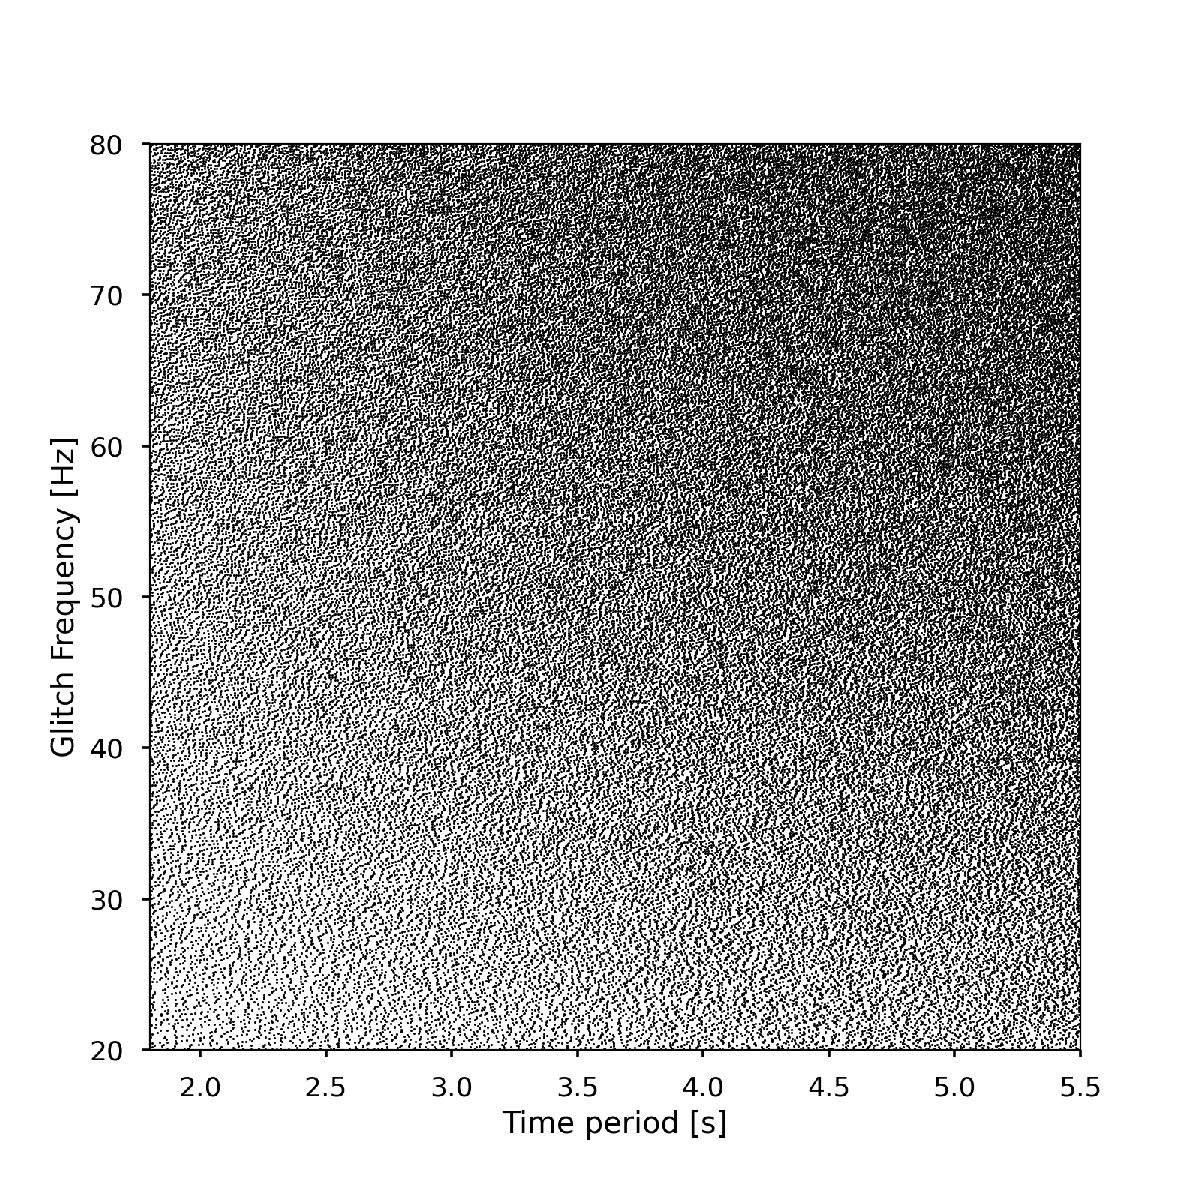
\includegraphics[width=1.0\textwidth]{images/4_archenemy/Section3/3.2/template_bank_square.pdf}
  \caption{The template bank of \scl{} glitch templates (black points) used in the search for \scl{} glitches. The \emph{glitch frequency} parameter values range from $20 \, \text{Hz}\text{--} 80 \, \text{Hz}$ and the \emph{time period} parameter values range from $1.8 \, \text{s}\text{--} 5.5 \, \text{s}$. This bank was created with a maximum match allowed between two templates of $0.97$ and contains 117,481 templates.}
  \label{4:fig:sq_bank}
\end{figure}

\subsection{Identifying potential \scl{} glitches in the data}

We test our method by searching through \gw{} data from 2019-11-18 16:13:05--2019-11-25 22:11:09 for the LIGO-Hanford and LIGO-Livingston detectors. This time corresponds to the 25th period of data used in the LVK analysis of O3 data for compact binary mergers~\cite{gwtc3:2023} and is prior to the implementation of RC tracking~\cite{reducing_scattering:2020} in these detectors. We only analyse data that is flagged as ``suitable for analysis" on the Gravitational Wave Open Science Center~\cite{GWOSC:2021}\footnote{We note that in O3 \emph{only} data suitable for analysis is released, so we simply analyse all of the publicly available data.}. This corresponds to 5.96 days of analysable data for LIGO-Hanford and 5.93 days for LIGO-Livingston.

Equipped with our template bank we now identify potential \scl{} glitches in the data. We matched filter all of the data against all of the templates, producing a signal-to-noise ratio time series for every template in the bank. These signal-to-noise ratio time series will contain peaks which, when above a certain limit, indicate the presence of a \scl{} glitch at a particular time. We retain any maxima within the time series that have a signal-to-noise ratio greater than 8. However, as we do this independently for every template, we will identify multiple peaks for any given glitch, and we will also find peaks that correspond to other types of glitch, or even \gw{} signals. We discuss how we reduce this to a list of identified \scl{} glitches in the following subsections.

\subsection{Scattered-light signal consistency test}

To prevent the search for \scl{} glitches from misclassifying other classes of glitches, or \gw{} signals, we employ a $\chi^2$ consistency test. The $\chi^2$ discriminator introduced in \cite{Allen_Chi:2005} divides \gw{} templates into a number of independent frequency bins. These bins are constructed so as to contain an equal amount of the total signal-to-noise ratio (SNR) of the original matched filter between template and data. The $\chi^{2}$ value is obtained by calculating the SNR of each bin, subtracting this from the expected SNR value for each bin and squaring the output. These values are summed for all bins and this value forms the $\chi^{2}$ statistic,
%
\begin{equation}
  \chi_{r}^{2} = \frac{\chi^{2}}{\textrm{DOF}} = \frac{n}{2n - 2} \sum_{i=1}^n \left(\frac{\rho}{\sqrt{n}} - \rho_{bin,i}\right)^2.
  \label{4:eqn:chi_squared}
\end{equation}
%
Here $n$ is the number of bins, $\rho$ is the SNR of the original matched filter between template and data, and $\rho_{bin}$ is the value of the SNR found when matched filtering one of the divided templates and the data. This test is constructed so as to produce large values when the data contains a glitch, or astrophysical signal, that is not well described by the template, but to follow a $\chi^2$ distribution if a glitch that matches well to the template is present, or if the data is Gaussian and stationary.

The $\chi^2$ test that we employ is similar to that of \cite{Allen_Chi:2005}, however compact binary merger waveforms increase in frequency over time whereas \scl{} glitch templates are symmetric about their centre. We therefore choose to construct our $\chi^2$ test with four non-overlapping bins \emph{in the time domain}, each of which contributes equally to the SNR, an example of the split template can be seen in figure \ref{4:fig:split_temp_subplot}. The matched filter between the bins and data is computed and the $\chi_{r}^{2}$ value is calculated using equation \ref{4:eqn:chi_squared} (where $n=4$). Any glitch, or astrophysical signal, which does not exhibit symmetric morphology should not fit with this deconstruction of the template, and should result in elevated $\chi_{r}^{2}$ values.

\begin{figure}
  \centering
  \begin{minipage}[t]{1.0\linewidth}
  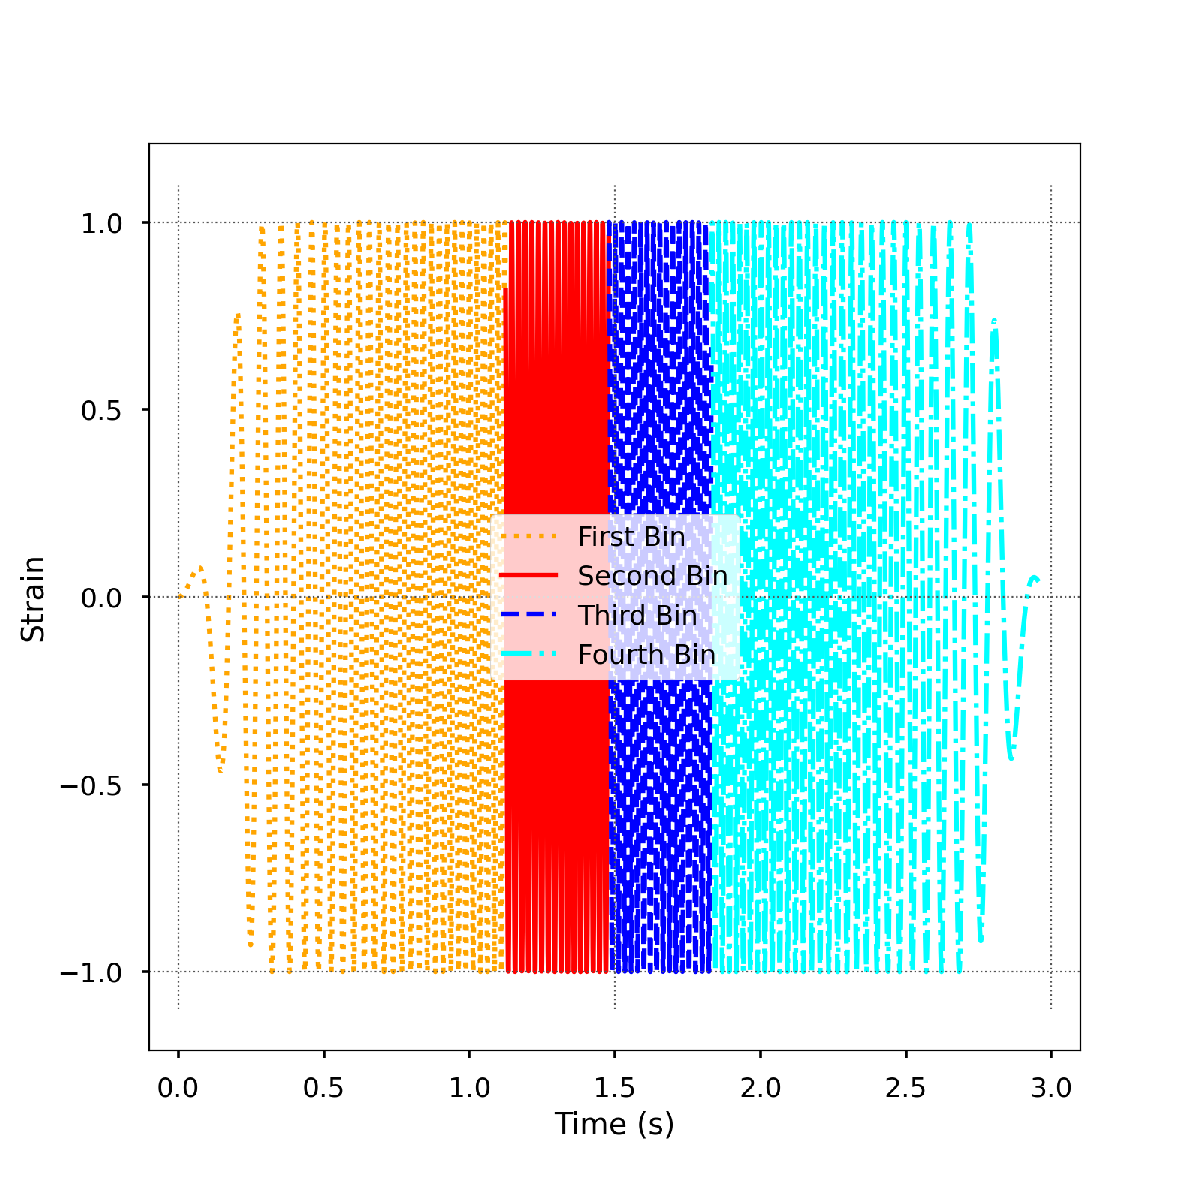
\includegraphics[width=0.49\textwidth]{images/4_archenemy/Section3/3.4/split_bins.pdf}
  \hspace{0.01\linewidth}
  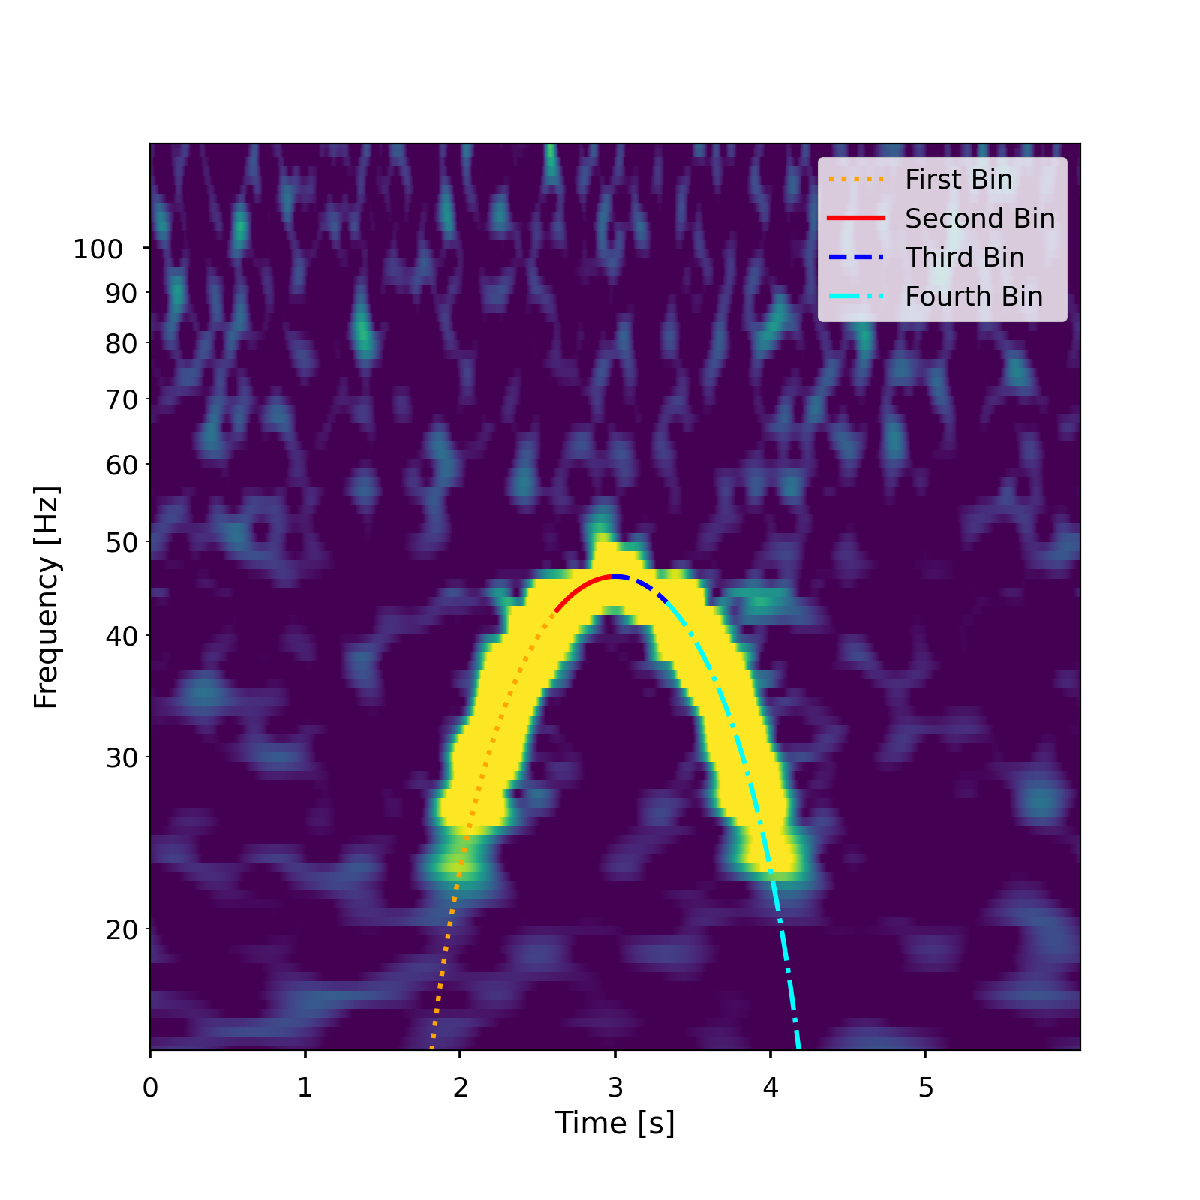
\includegraphics[width=0.49\linewidth]{images/4_archenemy/Section3/3.4/split_bins_qscan.pdf}
  \end{minipage}
  \caption{A \scl{} glitch template (left) where the colours and line-styles are indicative of the four equal SNR time bins to be used in calculating the $\chi_{r}^{2}$ value and re-weighting the SNR. The same \scl{} glitch template bins overlaid on an injection of the \scl{} glitch (right). The inner two bins are considerably shorter than the outer two bins which informs us that the center---higher frequency---region of the \scl{} glitch contributes a larger amount to the SNR per unit time than the lower frequency regions.}
  \label{4:fig:split_temp_subplot}
\end{figure}

After computing the $\chi_{r}^{2}$ value for potential \scl{} glitches, we follow~\cite{rw_snr_eq:2012} to compute a ``re-weighted signal-to-noise ratio'', which is an empirically tuned statistic depending on the signal-to-noise ratio and the $\chi_{r}^{2}$ value.  The re-weighting function we use matches that presented in~\cite{rw_snr_eq:2012},
%
\begin{equation}
\rho_{rw} =  \left\{  \begin{array}{l@{\quad}cr} 
\rho & \mathrm{if} & \chi_{r}^{2} \leq 1, \\  
\rho [(1 + (\chi_{r}^{2})^3)/2]^{-\frac{1}{6}} &  \mathrm{if} & \chi_{r}^{2} \ge 1,   
\end{array}\right.
\label{4:eqn:reweighting}
\end{equation}
%
where $\rho_{rw}$ represents the re-weighted signal-to-noise ratio of the \scl{} glitch template calculated using the signal-to-noise ratio, $\rho$, and the $\chi_{r}^{2}$ value of that template.
We do note that this re-weighting function has been tuned for compact binary merger waveforms and we did not repeat that tuning here with \scl{} glitches. One could retune this statistic, specifically targeting \scl{} glitches, using (for example) the automatic tuning procedure described in~\cite{McIsaac_Chi:2022}. However, we demonstrate the suitability of the $\chi^{2}$ test for our purposes in figure~\ref{4:fig:chi_snr} where we show the $\chi_{r}^{2}$ vs SNR distribution of the triggers found by our \scl{} glitch search when performed on data containing only \scl{} glitches and data containing a binary black hole \gw{} injection.

\begin{figure}
  \makebox[\textwidth][c]{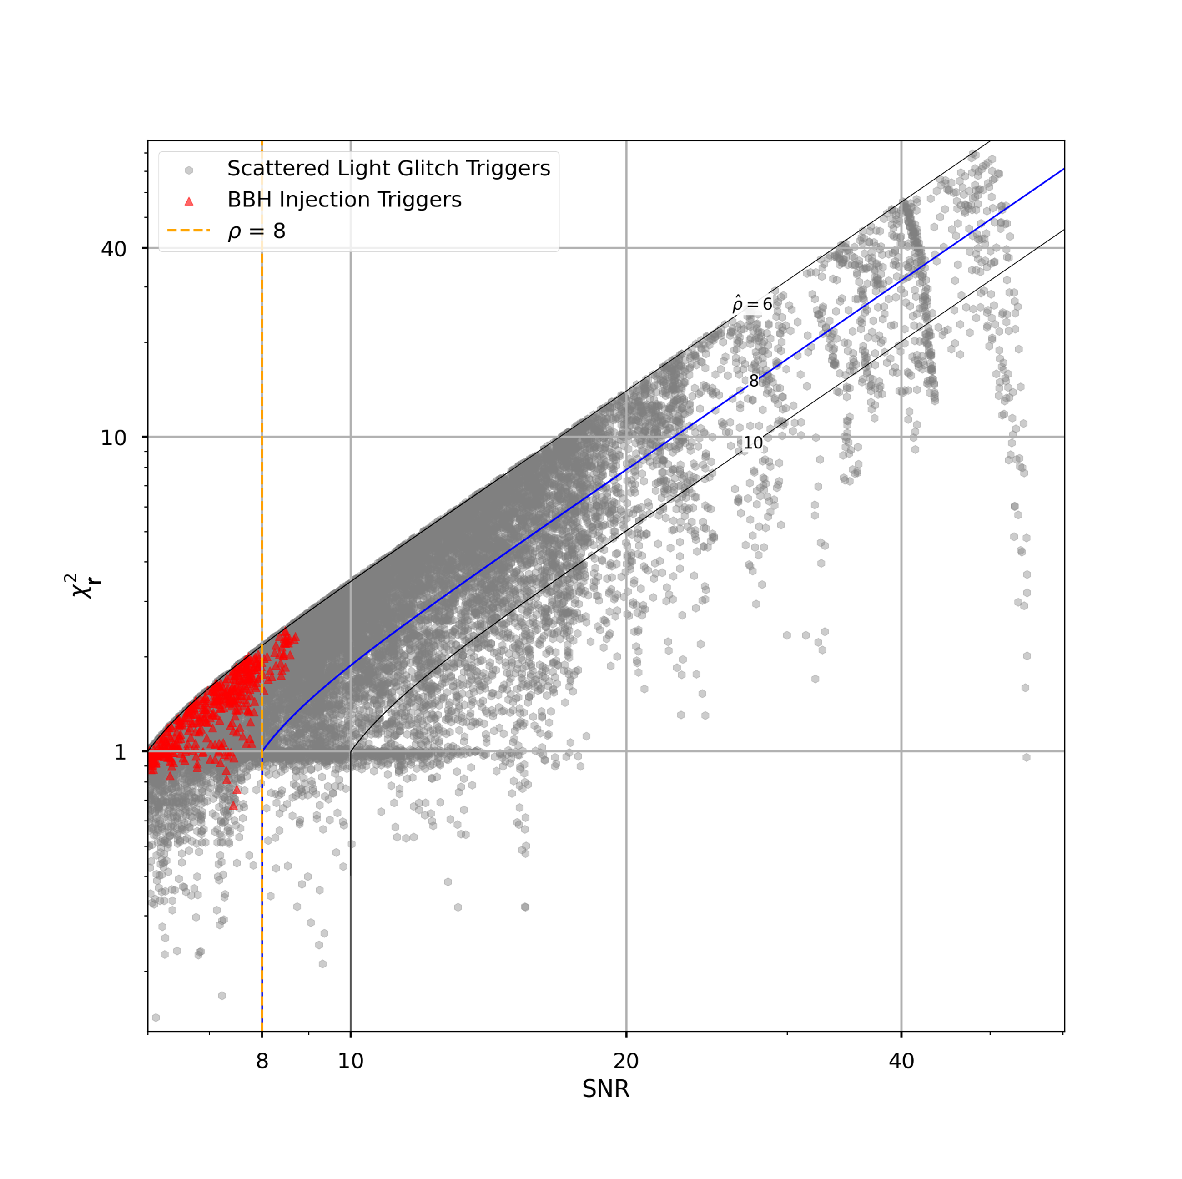
\includegraphics[width=\textwidth]{images/4_archenemy/Section3/3.4/SLvsBBH.pdf}}
  \caption{The signal-to-noise ratio and $\chi_{r}^{2}$ values for the triggers identified by the matched filtering and clustering of the \scl{} glitch template bank with data containing only \scl{} glitches (grey hexagons) and data containing a binary black hole \gw{} injection (red triangles). The black contour lines represent the re-weighted signal-to-noise ratio values the trigger will take when equation \ref{4:eqn:reweighting} is applied. The orange dashed vertical line indicates the signal-to-noise ratio value limit of 8, above which we decide to perform the $\chi^{2}$ test and calculate the re-weighted signal-to-noise ratio. The blue solid contour line indicates a re-weighted signal-to-noise ratio value of 8, which is the limit at which we consider the trigger to be real. Different re-weighting parameter values will produce different contour line shapes. It can be seen that no triggers for the data containing the \gw{} injection lie beneath the contour line and therefore no \scl{} glitches are found on the \gw{} signal.}
  \label{4:fig:chi_snr}
\end{figure}

We note that the $\chi^{2}$ test increases the number of matched filters required by the search and therefore the computational cost of the search. Each template would require the matched filtering of an additional $4$ ``binned'' templates to calculate the $\chi_{r}^{2}$ value to re-weight the SNR time series of that template, increasing computational cost by a maximum factor of $5$. However, we reduce this increase by only computing the $\chi^{2}$ where it is needed, specifically for any template where the SNR time series has values above the threshold of 8.

\subsection{Identifying all \scl{} glitches in the data}

\begin{figure}
      \begin{minipage}[t]{1.0\linewidth}
        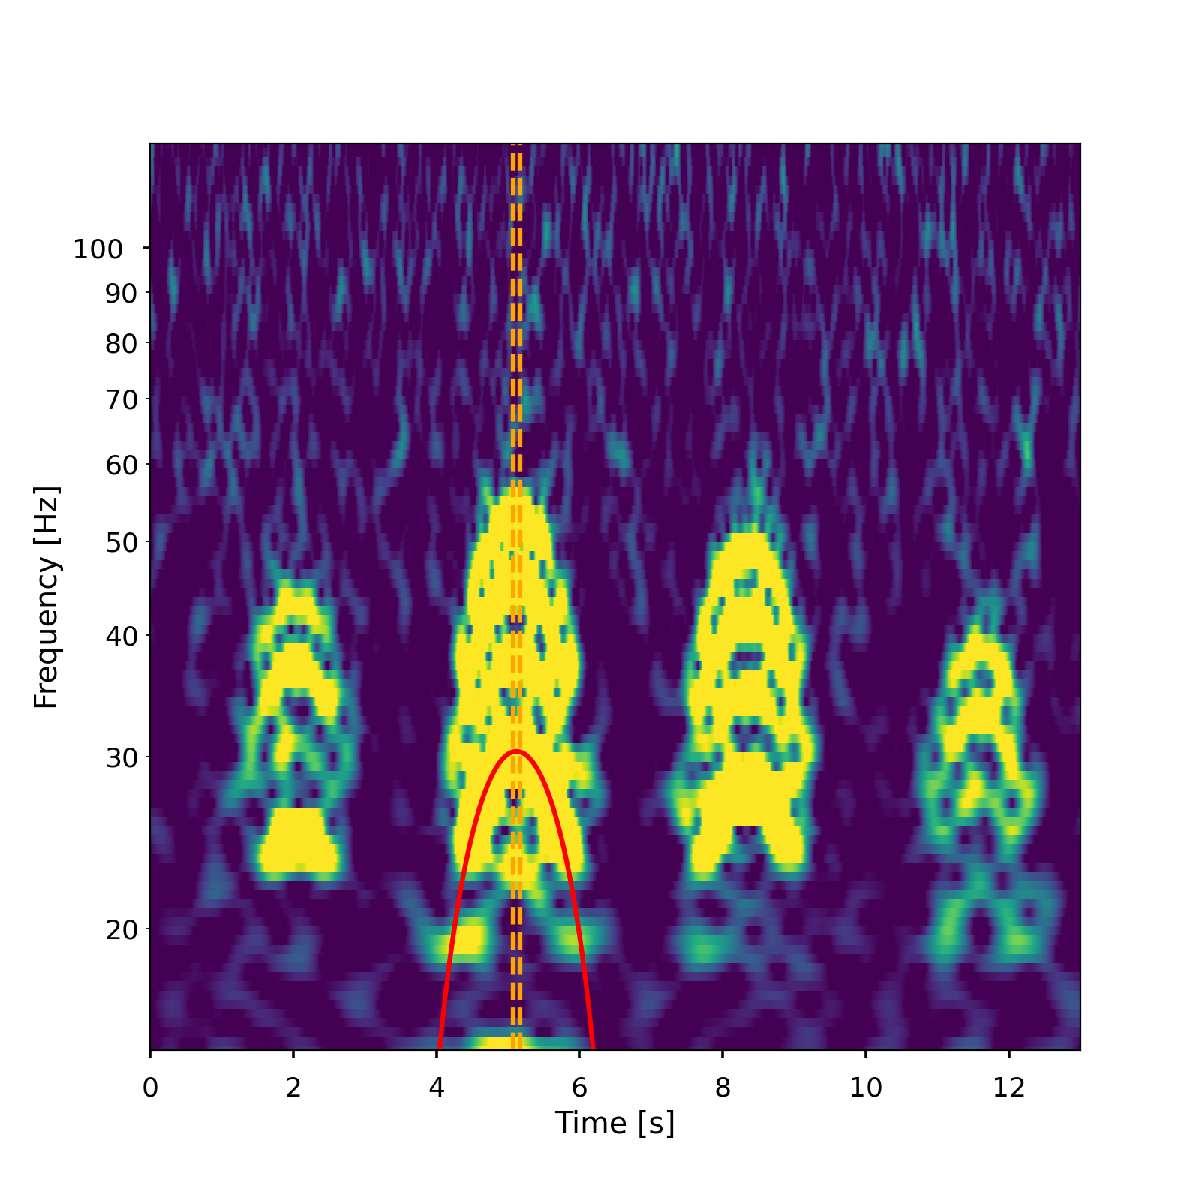
\includegraphics[width=0.49\linewidth]{images/4_archenemy/Section3/3.5/cluster_qscan.pdf}
        \hspace{0.01\linewidth}
        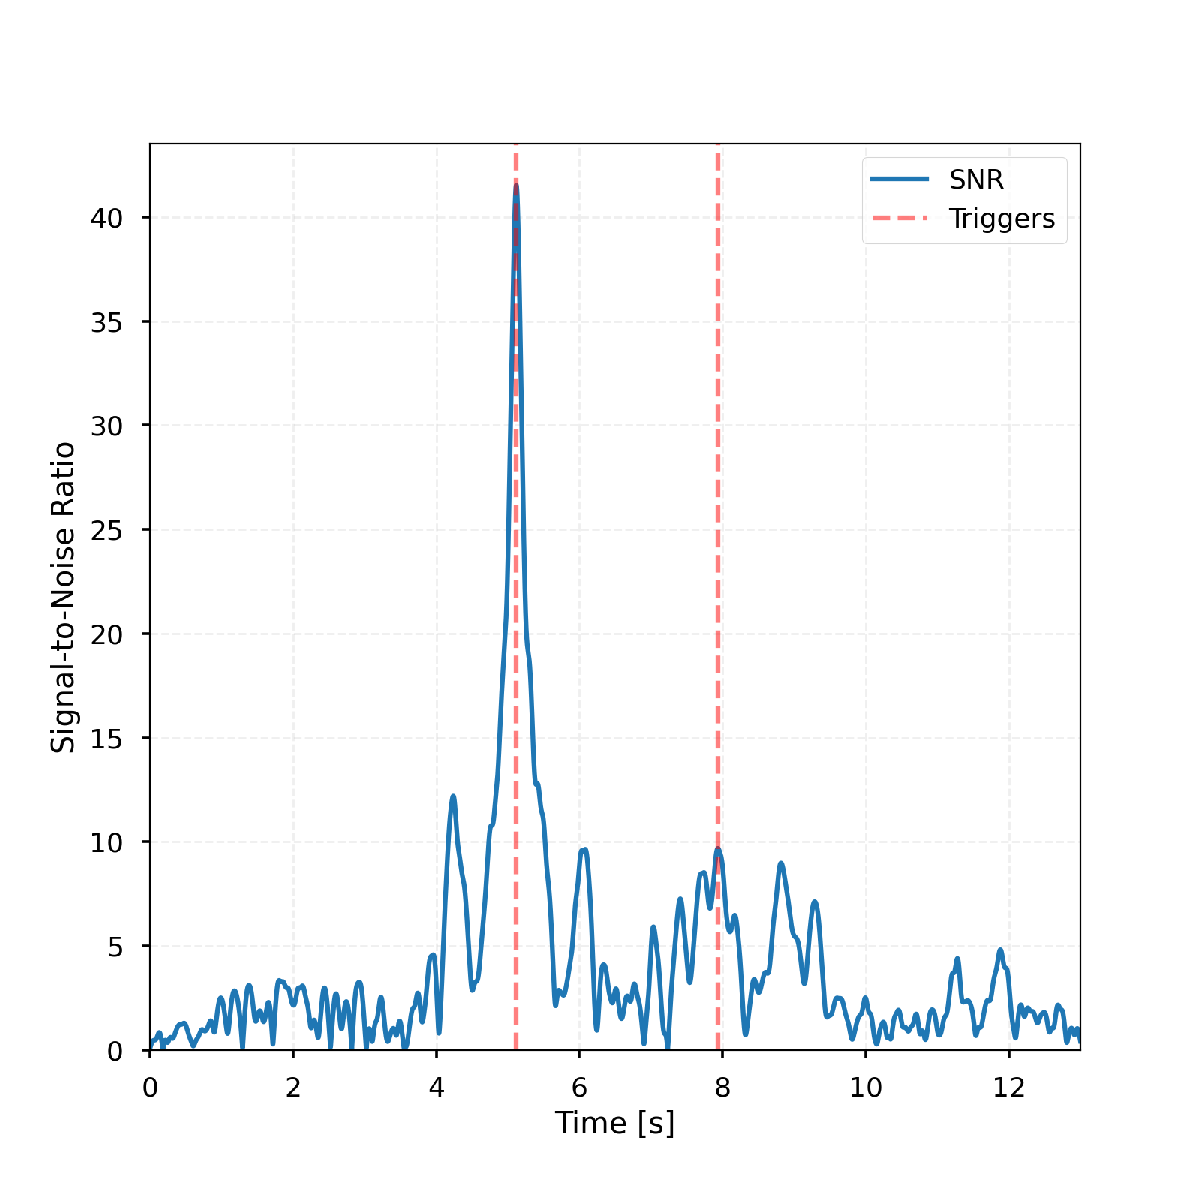
\includegraphics[width=0.49\linewidth]{images/4_archenemy/Section3/3.5/cluster_snr_ts.pdf}
      \end{minipage}
      \begin{minipage}[t]{1.0\linewidth}
        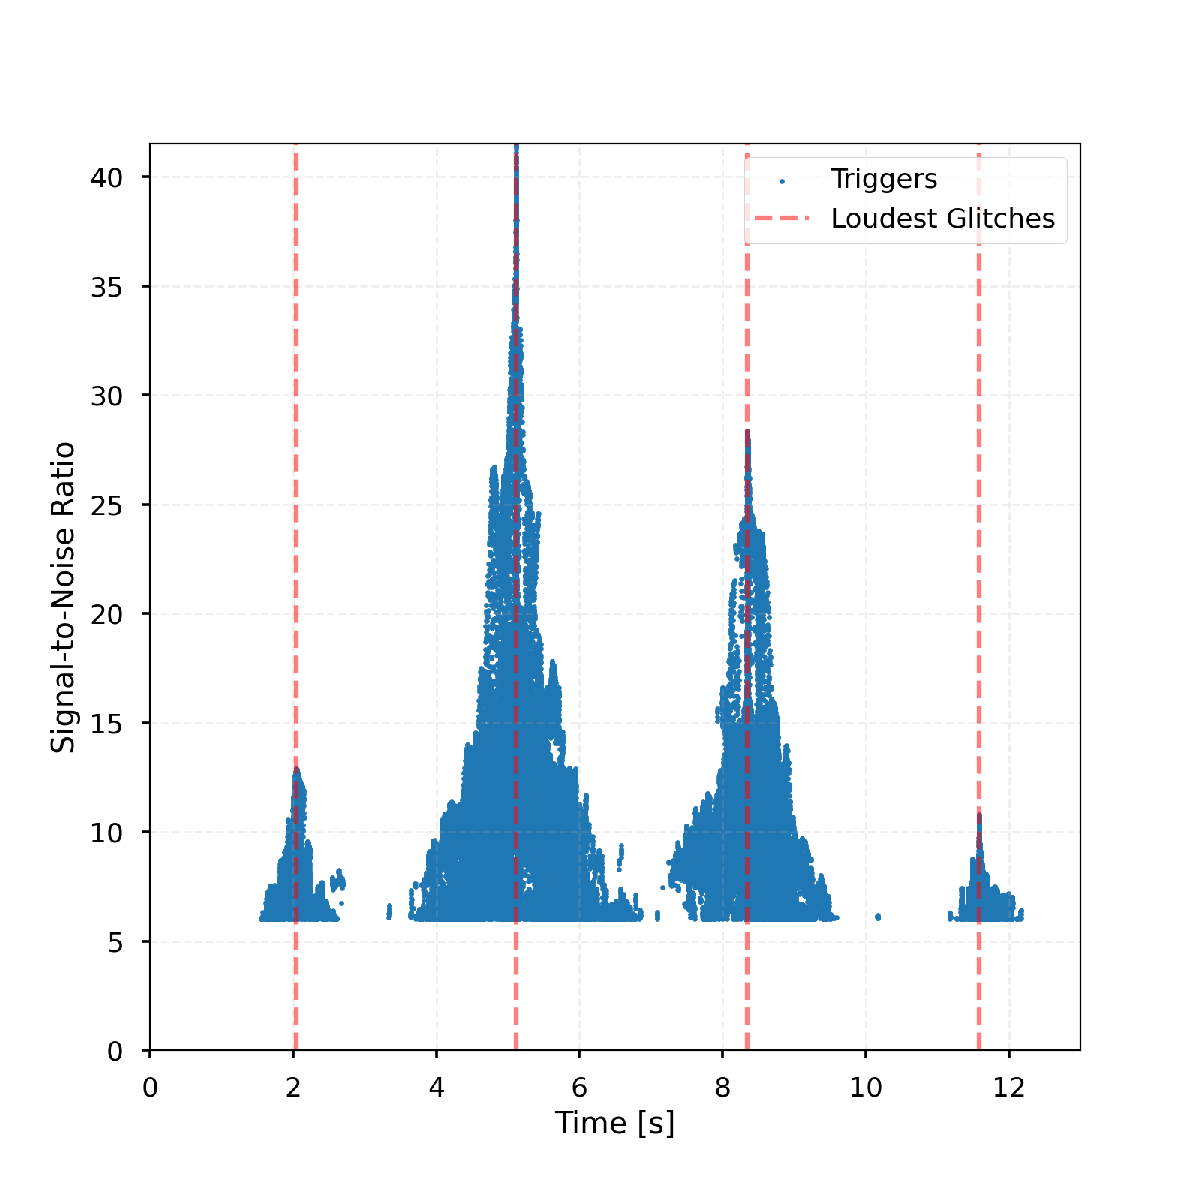
\includegraphics[width=0.49\linewidth]{images/4_archenemy/Section3/3.5/cluster_all_triggers.pdf}
        \hspace{0.01\linewidth}
        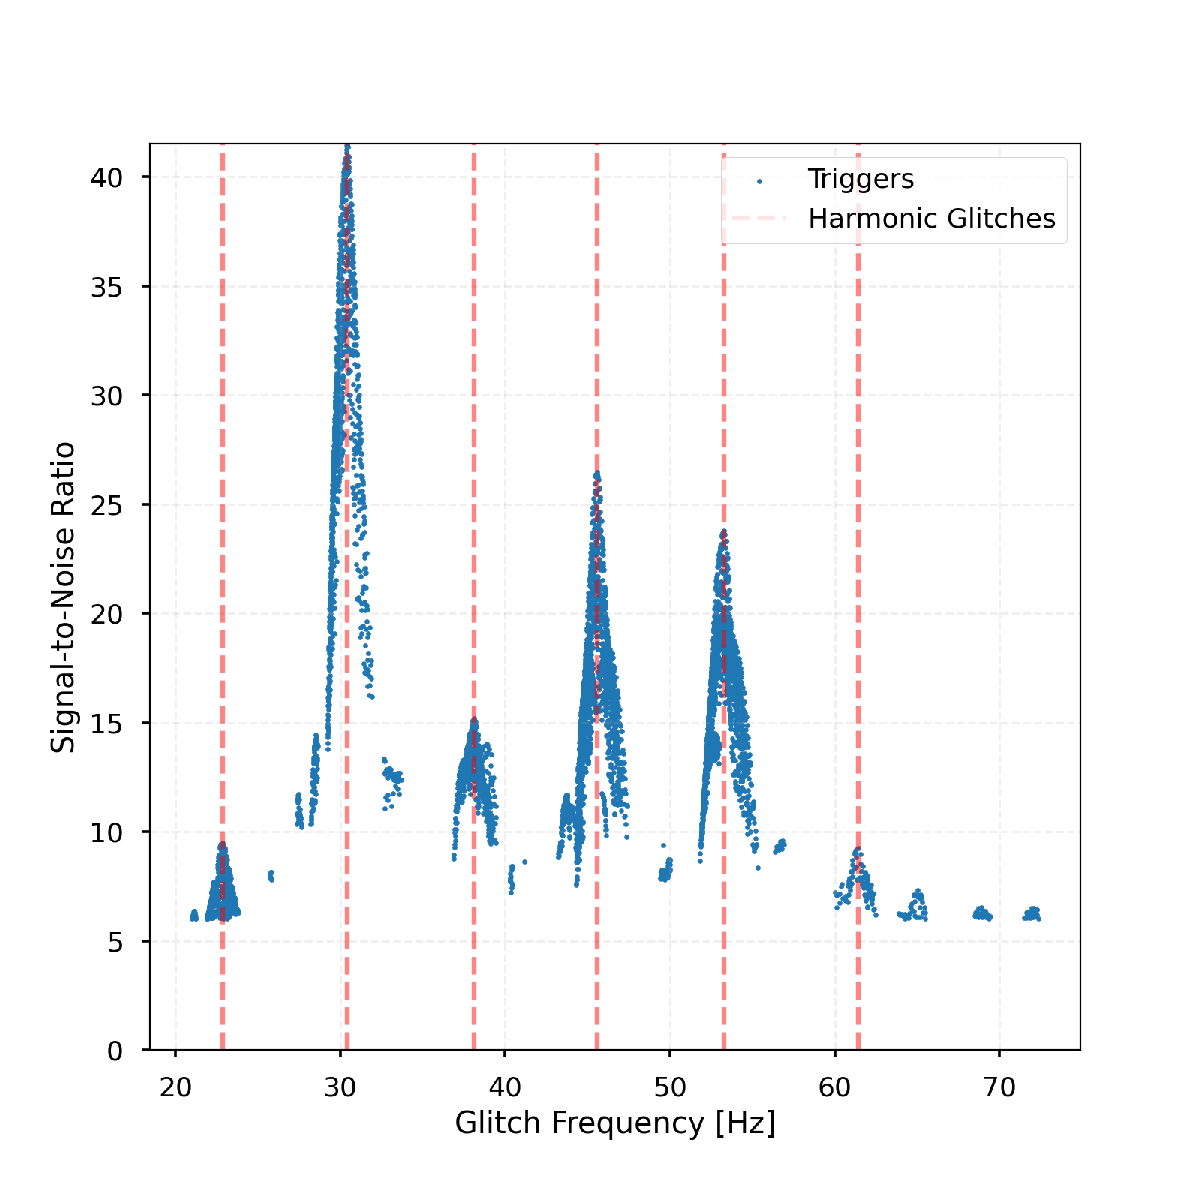
\includegraphics[width=0.49\linewidth]{images/4_archenemy/Section3/3.5/cluster_in_frequency.pdf}
      \end{minipage}
    \caption{The process for identifying all the \scl{} glitches in a period of \gw{} data. The red overlay in the \gw{} data used in this example (top left) indicates the highest re-weighted signal-to-noise trigger found, the dashed vertical lines represent the time slice window around this trigger. The re-weighted signal-to-noise ratio time series resulting from the matched filter of this trigger's template and the data (top right) is clustered in time to identify the triggers found above a signal-to-noise threshold of $8$, indicated by red vertical dashed lines. All the triggers from all of the templates in the template bank are then clustered in time (bottom left) to identify the highest re-weighted signal-to-noise glitches in the data, indicated by the orange vertical dashes lines. The triggers found within the time slice window, with a similar \emph{time period} value---within $\pm 10\%$---of the highest re-weighted signal-to-noise ratio trigger (bottom right) are clustered by their \emph{glitch frequency} value to find the harmonic glitches at the same time, indicated again by red dashed lines.}
    \label{4:fig:clustering_story}
\end{figure}

Our matched filtering process retains ``triggers'' (potential \scl{} glitches) wherever the re-weighted signal-to-noise time series is larger than 8. We retain no more than one trigger within a window size equal to half the \emph{time period} of the template used to produce the re-weighted signal-to-noise time series and only store triggers at local maxima. A re-weighted signal-to-noise time series with multiple peaks and identified triggers can be seen in the top right panel in figure \ref{4:fig:clustering_story}.

After matched filtering all the templates against the data we will recover multiple triggers for any potential \scl{} glitch, as we might expect to independently identify peaks in multiple templates around the true values of the glitch. We therefore collect all of the triggers generated by the template bank and cluster these in time, using a window of half of the shortest duration template---$0.9$ seconds. This will result in a list of triggers corresponding to the highest re-weighted signal-to-noise ratios, where each trigger should correspond to a unique \scl{} glitch. The bottom left panel in figure \ref{4:fig:clustering_story} shows an example of the triggers found by the search and the highest re-weighted signal-to-noise ratio triggers found by clustering.

However, we also expect to see instances of harmonic glitches which are produced by the same scattering surface and so share the same \emph{time period} and have \emph{glitch frequency} values equal to a multiple of the lowest frequency glitch in the harmonic stack~\cite{TAccadia:2010}. We investigate each trigger in the list, searching for harmonic glitches occurring at the same time. We use the first list of triggers identified by all templates across the bank and filter by those that occur within $\pm0.05$ seconds of the \emph{center time} of the trigger we are investigating, an example of this window can be seen in the top left panel of figure \ref{4:fig:clustering_story}. We then filter the triggers again, keeping only those with an associated \emph{time period} value within $\pm 10 \%$ of the trigger's \emph{time period}. Finally we cluster these remaining triggers by their associated \emph{glitch frequency} using a window size of $4$Hz, a lower limit on the frequency separation of harmonic glitches, the bottom right panel in figure \ref{4:fig:clustering_story} shows the identification of harmonic glitches for the overlaid \scl{} glitch in the top left panel of figure \ref{4:fig:clustering_story}.

\subsection{Hierarchical subtraction to find parameter values}

We now have a list of identified \scl{} glitches and their parameter values, however, these might not be fully accurate when there are many glitches close in time and frequency, as illustrated in figure~\ref{4:fig:overlay_goods}. It is important that the parameters we find match well with the glitches in the data to remove as much power as possible.

To better identify the parameter values of the \scl{} glitches, we perform a hierarchical procedure using information about the glitches we have found so far. Firstly, we create new segments of time which we know contain \scl{} glitches, taking a window of $8$ seconds on either side of each previously identified glitch, if two glitch windows overlap they are combined into the same segment.

For each segment we then create a reduced template bank, consisting of templates ``close'' to the \scl{} glitches previously identified in the segment. We take the smallest and largest \emph{time period} and \emph{glitch frequency} glitches in the segment and bound the retained templates by these values with $\pm 0.25$ seconds on the \emph{time period} and $\pm 1$Hz on the \emph{glitch frequency}. For each data segment the reduced template bank is matched filtered with the data, the maximum re-weighted SNR value is found and the corresponding glitch is subtracted. We then matched filter \emph{again} and remove the next largest re-weighted SNR template. This process is repeated until no templates, when matched filtered with the data, produce any re-weighted SNR values above the SNR limit of $8$. This method of hierarchical subtraction produces our final list of \scl{} glitches.

A further benefit of using these shorter data segments is that we are estimating the PSD of the data using only a short period of data close to the \scl{} glitches being removed. This protects us from a rapidly changing PSD in non-stationary data, which might cause Gaussian noise to be identified with larger SNR in the periods where the PSD is larger. This can be resolved by including the variation in the power spectral density as an additional statistic in the re-ranking of triggers, which has been done for compact binary coalescence \gw{} searches in~\cite{PSD_var:2020}.

We demonstrate the hierarchical subtraction step on an amount of data which contains four injected \scl{} glitches in a single harmonic stack, this can be seen in figure \ref{4:fig:injected_glitches}. As shown, the \scl{} glitches are found and subtracted from the data leaving behind a cleaned segment of \gw{} data with no excess noise. Figure~\ref{4:fig:overlay_goods} shows the identified \scl{} glitch triggers before and after performing the hierarchical subtraction step on a stretch of data containing real \scl{} glitches. We identify more triggers prior to performing hierarchical subtraction, however there are more errant mismatches between \scl{} glitches and the overlaid templates. By performing the hierarchical subtraction, we more accurately identify \scl{} glitches, however, we miss some glitches that were previously identified. There is still some imperfection in this process and we do not refine the method further in this work, but highlight this as useful direction for future studies in removing \scl{} glitches. 

\begin{figure}
     \centering
     \begin{minipage}[t]{1.0\linewidth}
        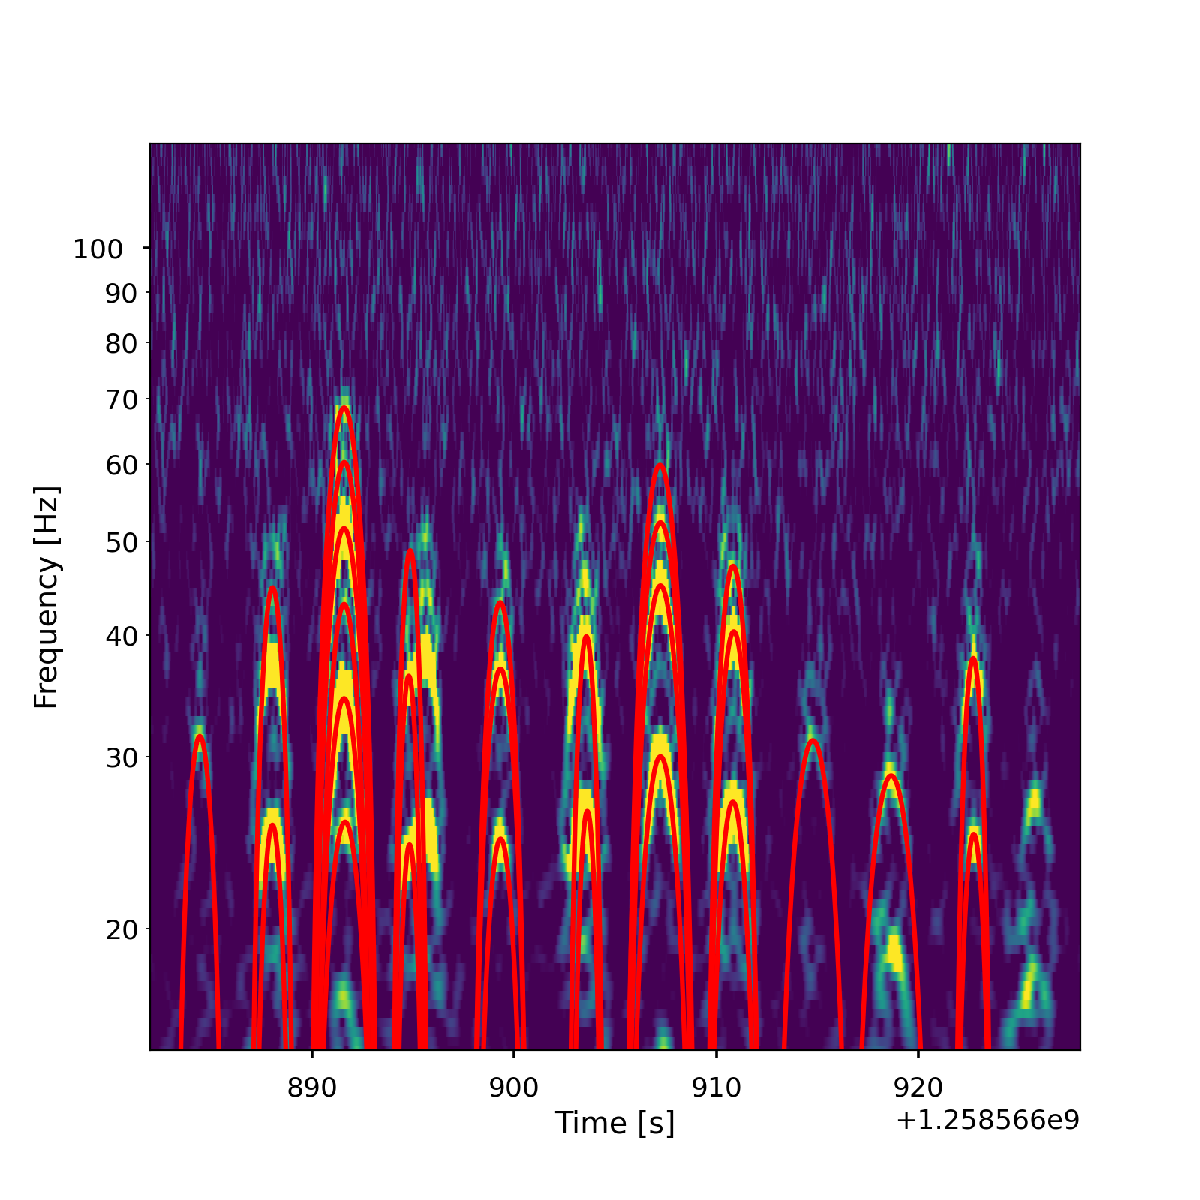
\includegraphics[width=0.49\linewidth]{images/4_archenemy/Section3/3.6/overlay_good_overlays_first.pdf}
        \hspace{0.02\linewidth}
        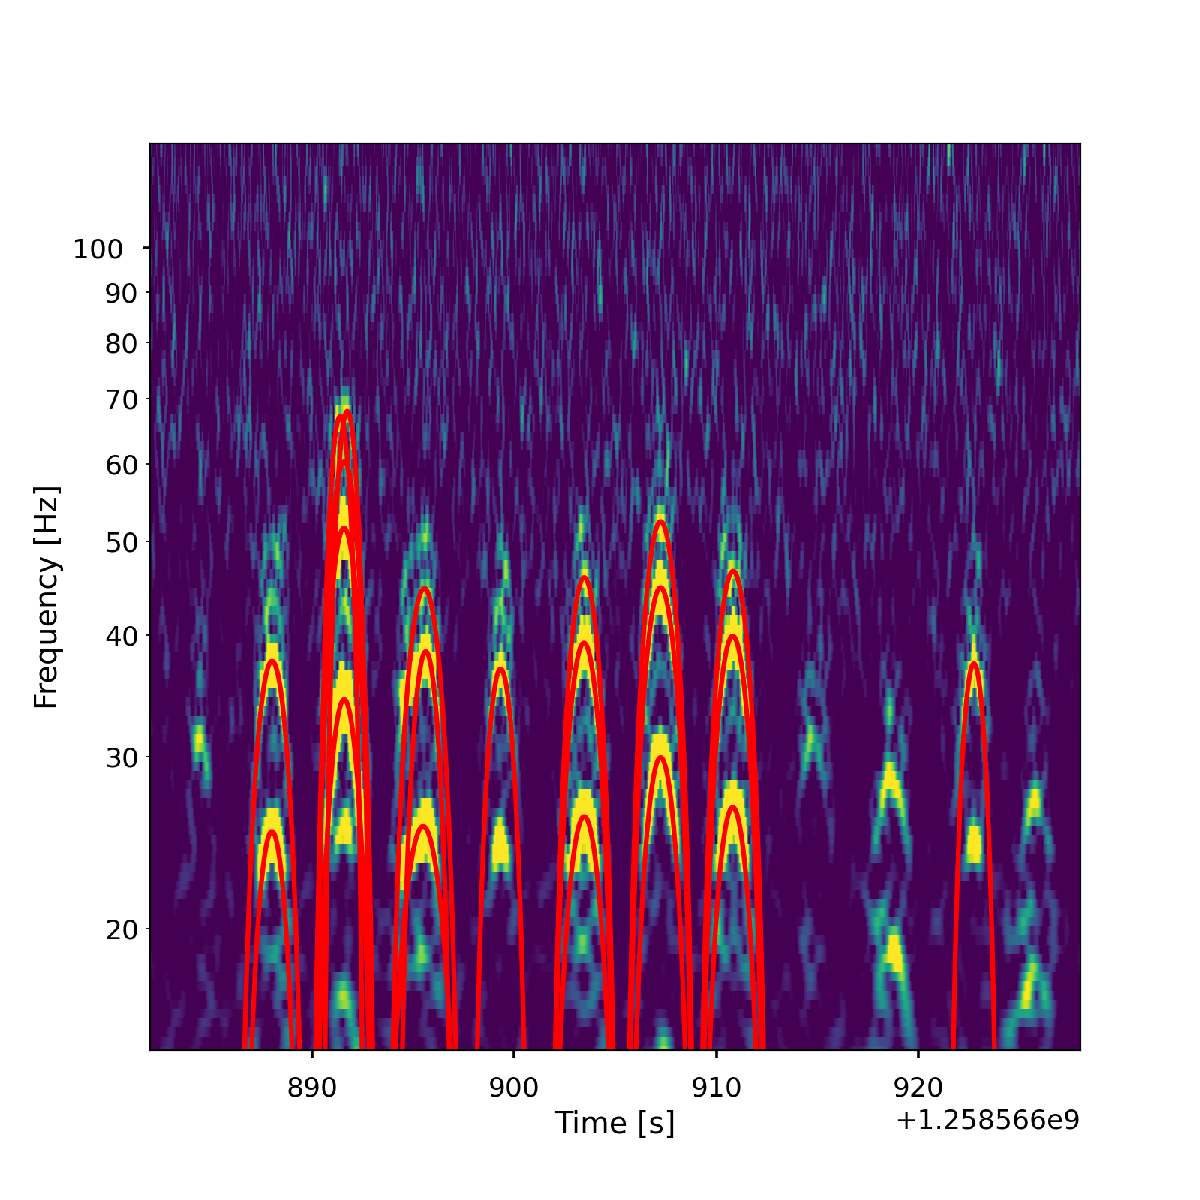
\includegraphics[width=0.49\linewidth]{images/4_archenemy/Section3/3.6/overlay_good_overlays_second.pdf}
     \end{minipage}
         \caption{LIGO-Hanford data from 2019-11-23 17:54:22--2019-11-23 17:55:12 containing \scl{} glitches which have been identified by the ArchEnemy search (left), there is a misalignment in the template found for a number of glitches in this period of data and some missed glitches. \Scl{} glitches remaining after running the hierarchical subtraction search (right) for the same period of data, we have missed more \scl{} glitches however misalignments have been removed. The highest harmonic at approximately $892$ seconds has been incorrectly split into two separate templates.}
    \label{4:fig:overlay_goods}
\end{figure}

\begin{figure}
     \centering
     \begin{minipage}[t]{1.0\linewidth}
        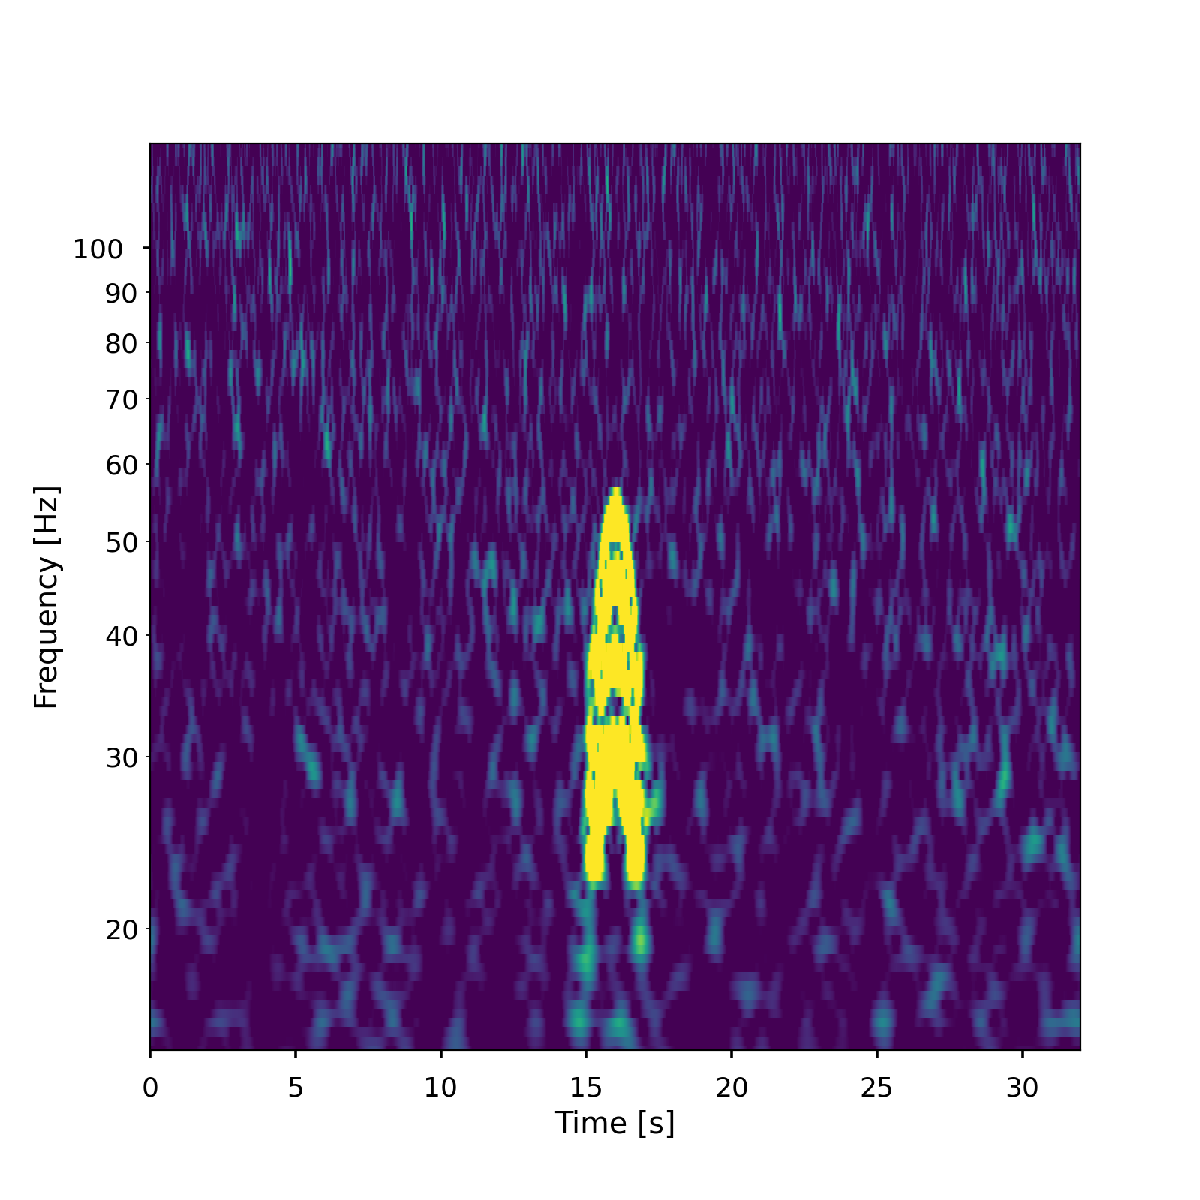
\includegraphics[width=0.49\linewidth]{images/4_archenemy/Section3/3.6/injected_artefacts_initial.pdf}
        \hspace{0.02\linewidth}
        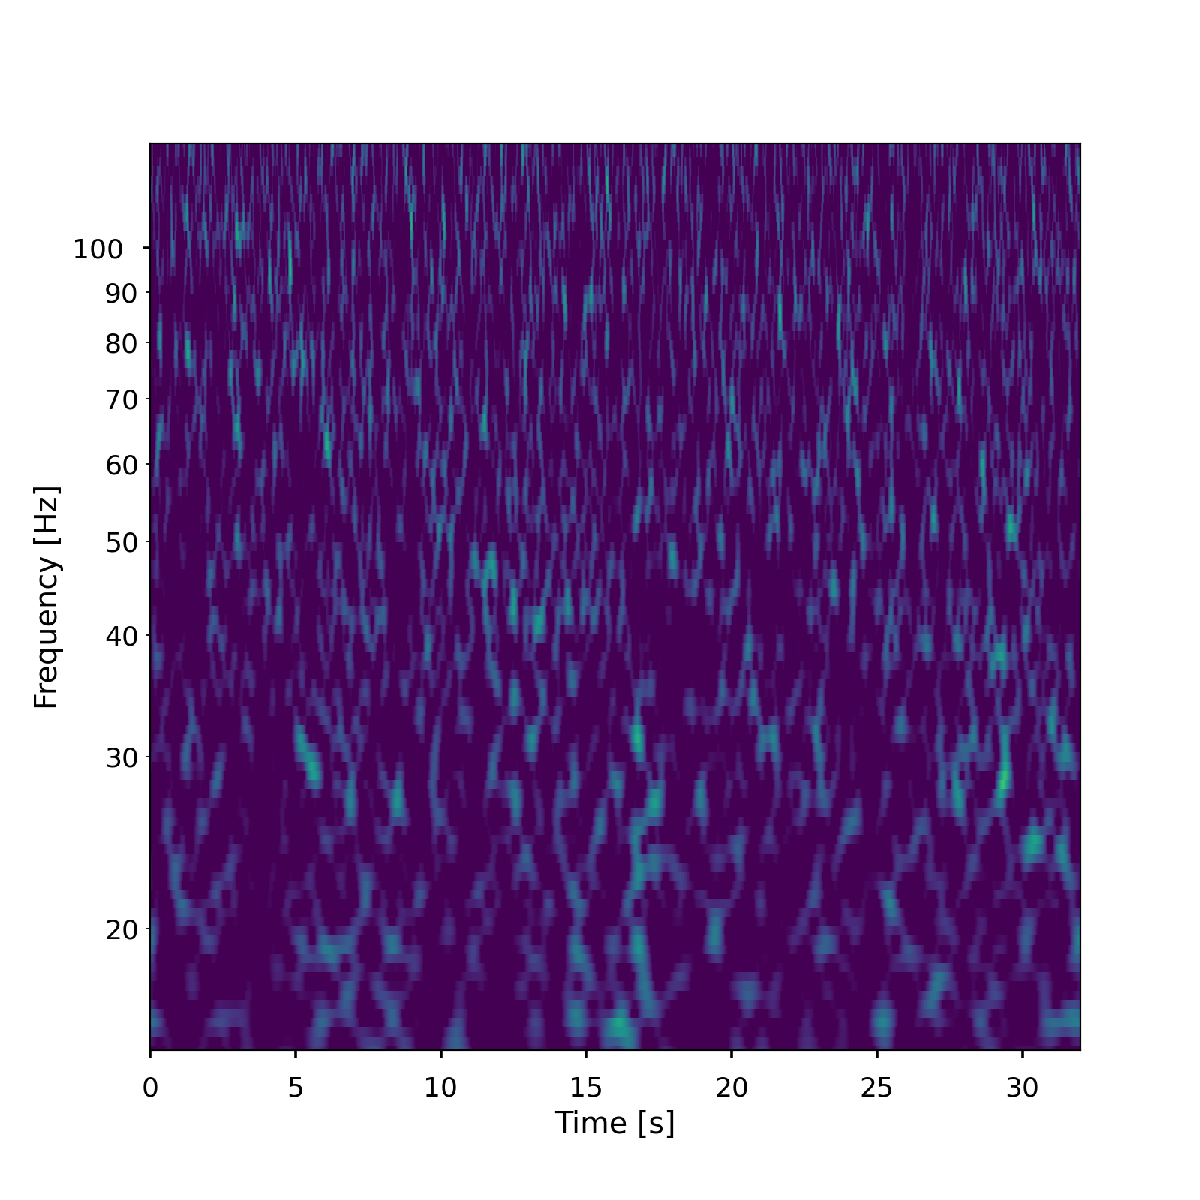
\includegraphics[width=0.49\linewidth]{images/4_archenemy/Section3/3.6/injected_artefacts_subtracted.pdf}
     \end{minipage}
         \caption{Data containing an injected stack of harmonic \scl{} glitches (left) and the corresponding data found when running the hierarchical subtraction search and subtracting the identified \scl{} glitches from the data (right).}
    \label{4:fig:injected_glitches}
\end{figure}

\subsection{Identified \scl{} glitches}

The methodology described in previous sections is implemented in our ``ArchEnemy'' pipeline, which is capable of searching for \scl{} glitches in \gw{} data using a pre-generated bank of glitch templates. We use ArchEnemy to analyse the aforementioned data, which produced a list of $2749$ \scl{} glitches in data from the LIGO-Hanford observatory and $1306$ from the LIGO-Livingston observatory.

The number of \scl{} glitches found by the ArchEnemy pipeline can be compared to Gravity Spy for the same period of time. Gravity Spy finds $2731$ and $1396$ for LIGO-Hanford and LIGO-Livingston respectively~\cite{gravityspy:2023}. There will be a difference in the number of glitches found by ArchEnemy and Gravity Spy for at least two reasons: Gravity Spy treats an entire stack of harmonic glitches as a single \scl{} glitch whereas ArchEnemy will identify each glitch as a separate occurrence. Gravity Spy can also identify \scl{} glitches which are not symmetric and fall outside our template bank, for example, the \scl{} glitches shown in figure~\ref{4:fig:overlay_bads}.

Figure~\ref{4:fig:overlay_goods} is an example of the results of the ArchEnemy pipeline and how well it has identified \scl{} glitches in a period of data. A majority of the glitches have been identified with the correct parameter values and even in cases where the chosen template is not visually perfect, there is a good match between the template and the identified power in the data, particularly in the case of slightly asymmetric glitches. Figure~\ref{4:fig:overlay_bads} demonstrates a period of time where the ArchEnemy pipeline has not fitted well the \scl{} glitches in the data. The glitches at this time are improperly fit by the templates due to asymmetry of the morphology of the glitches and because some of the glitches are outside of our template bank parameter range. However, we note that this is a very extreme period of \scl{} glitching and immediately after this time the detector data is no longer flagged as ``suitable for analysis''.

\begin{figure}
       \centering
    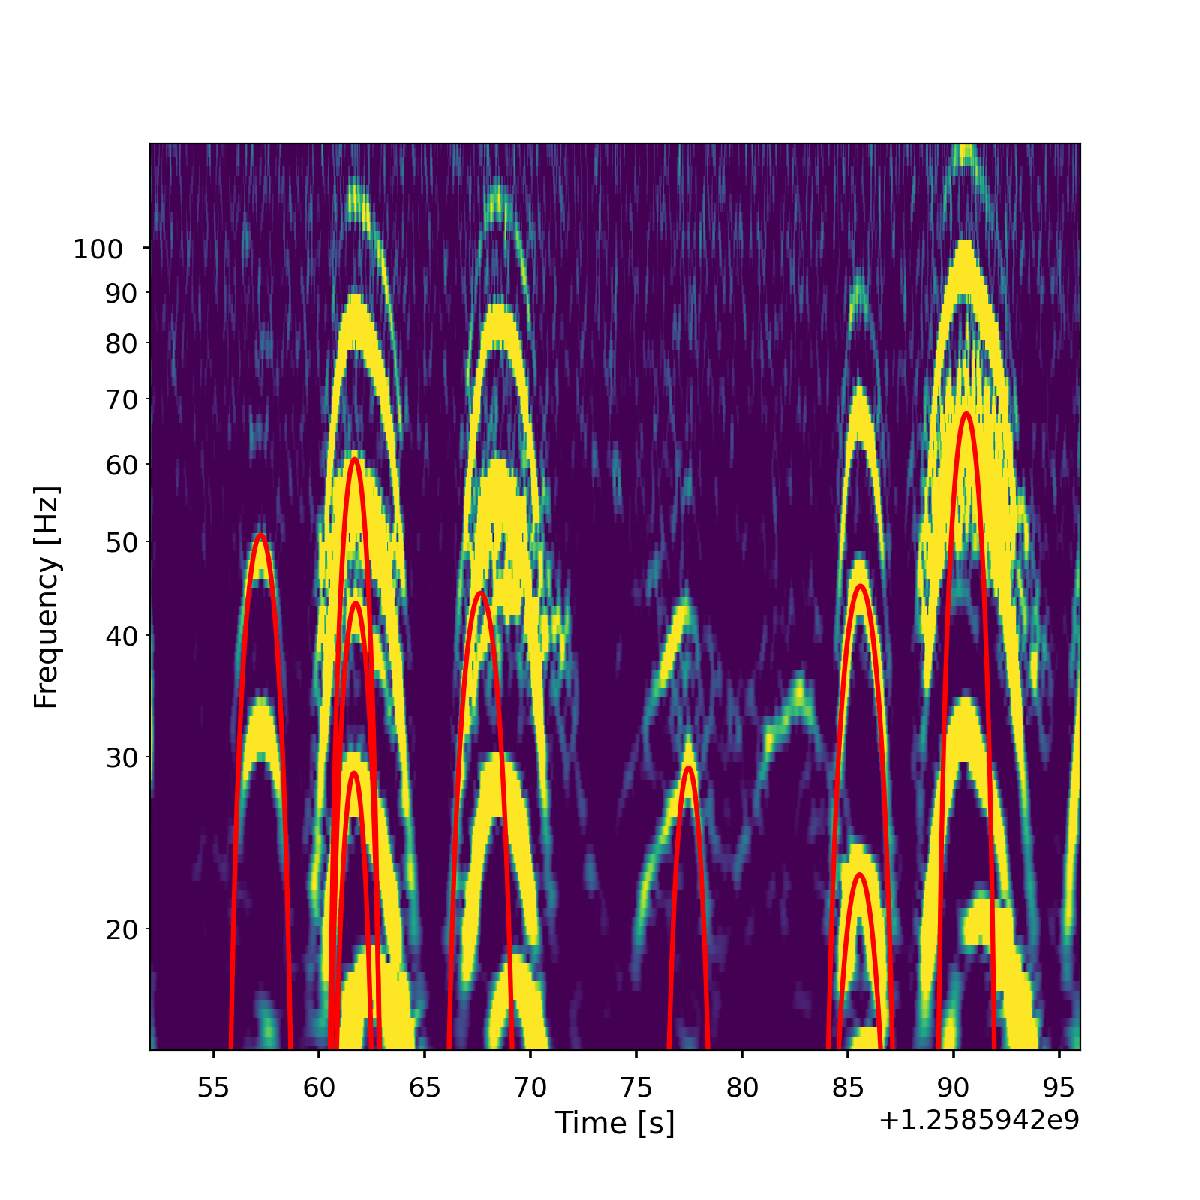
\includegraphics[width=0.7\linewidth]{images/4_archenemy/Section3/3.7/overlay_bad_overlays.pdf}
    \caption{LIGO-Livingston data from 2019-11-24 01:30:32--2019-11-24 01:31:20 containing a very large number of \scl{} glitches at multiple times and frequencies over-plotted with the \scl{} glitches identified by the ArchEnemy search. Very few overlays match well onto \scl{} glitches. The template bank used in this search terminates at $80$ Hz and so the \scl{} glitches located above this value will not be correctly identified. There are also asymmetric \scl{} glitches located which will not be identified correctly by our search which assumes symmetry in the \scl{} glitch.}
    \label{4:fig:overlay_bads}
\end{figure}

We have demonstrated the ArchEnemy pipeline on a stretch of data from O3 and have identified and characterised a list of \scl{} glitches, which could be removed from the data. We do note that there are cases where the identification has not worked well, but we expect that subtracting our list of glitches from the data will reduce their effect on the \gw{} search. In the next section we will demonstrate this by quantifying sensitivity with the PyCBC pipeline.

\subsection{Safety of \scl{} identification}
\label{4:ssec:injsafety}

The data we have searched through contains no previously identified \gw{} signals~\cite{gwtc3:2023}. However, there is a risk that the ArchEnemy search would identify real \gw{} signals as \scl{} glitches. To assess this possibility we simulate and add a large number of \gw{} signals into the data and assess whether any signals are misidentified.

To do this, we use three separate sets of simulated \gw{} signals (or ``injection sets''), one for BBHs, another for binary neutron stars (BNSs) and a third for neutron star black hole (NSBH) systems. We use the same simulations as the LVK search of this data, detailed in the appendix of~\cite{gwtc3:2023}. Each injection set consists of $6200$ simulated signals spaced between $82$ and $120$ seconds apart. We treat these injection sets exactly the same as for the injection-less data, adding the simulations to the data, and then running ArchEnemy to produce a list of \scl{} glitches for each injection set.

To determine whether we have misidentified any \gw{} injections as \scl{} glitches we look for glitches we have found within the overlapping frequency band of \gw{} signals and our \scl{} glitch template bank. This corresponds to approximately $15$ second before merger time for the injections. The simulated signals occur every ${\sim}100$ seconds so we expect to see glitches within this $15$ second window, therefore, we also require that there must be more triggers identified in the \scl{} glitch search \emph{with} injections when compared to the search \emph{without} injections within the window. The details of the number of \gw{} injections with overlapping \scl{} triggers can be seen in table~\ref{4:tab:coincident_triggers}.

\begin{table}[tb]
\caption{\label{4:tab:coincident_triggers}For both interferometers and all $3$ injection sets we identify the number of injections which are found to have \scl{} glitches identified within $15$ seconds of merger time (``Injections with Coincident Triggers''), along with the number of \scl{} glitches found within this window for these injections (``Scattered-Light Coincident Triggers''). We investigated each of these injections and recorded the number which actually had \scl{} glitches identified due to the injected \gw{} signal (``Actual Overlapped Injections'').}
\footnotesize
\renewcommand{\arraystretch}{1.2}
\begin{tabular}{@{}cccccc}
\hline
&    & Injections with& Scattered-Light & Actual Overlapped \\
Interferometer & Injection Set & Coincident Triggers& Coincident Triggers&Injections \\
\hline
H1 & BBH           & 20 & 45 & 1\\
   & BNS           & 23 & 50 & 2\\
   & NSBH          & 38 & 73 & 7\\
L1 & BBH           & 13 & 21 & 2\\
   & BNS           & 18 & 30 & 2\\
   & NSBH          & 35 & 56 & 16\\
\hline
\end{tabular}

\end{table}

A \scl{} glitch will be identified close to a \gw{} signal in two cases: the ArchEnemy search is misidentifying the \gw{} signal as a glitch \emph{or} the simulated signal was added close to actual glitches and a change in the data has meant a different number of glitches has been identified. The presence of real \scl{} glitches means we might miss a \gw{} signal, therefore, we \emph{do} want to find and subtract glitches close to \gw{} signals, but we do not want to subtract power from the \gw{} signal itself. The \scl{} glitch $\chi^{2}$ test was designed to prevent the matching of \scl{} glitch templates on other causes of excess power, however, these results show it is not perfect.

We investigate each injection with coincident \scl{} triggers, seeing how many had misidentified \scl{} glitches on the inspiral of the \gw{} signal, this number can be seen in the column ``Actual Overlapped Injections'' in table~\ref{4:tab:coincident_triggers}. We have included an example of the matching of \scl{} glitches onto \gw{} injections in figure~\ref{4:fig:loud_inj}, the right panel shows the \gw{} data post glitch subtraction where it can be seen there is a portion of the power being subtracted from the signal. Although power is being removed from the signal, the \gw{} injection is still found by the search for \gws{}, which we will describe later. For the cases that we have investigated, we note that the behaviour shown in figure~\ref{4:fig:loud_inj} only happens for signals that have very large signal-to-noise ratio, and are therefore unphysically close to us. A similar effect is observed with the ``autogating'' process, described in~\cite{PyCBC:2016}, which prevents the detection of these loud signals. In contrast to the ``autogating'' though, signals like that illustrated in figure~\ref{4:fig:loud_inj} are still identified as \gw{} signals by the PyCBC search after \scl{} glitch removal.

\begin{figure}
  \centering
  \begin{minipage}[t]{1.0\linewidth}
    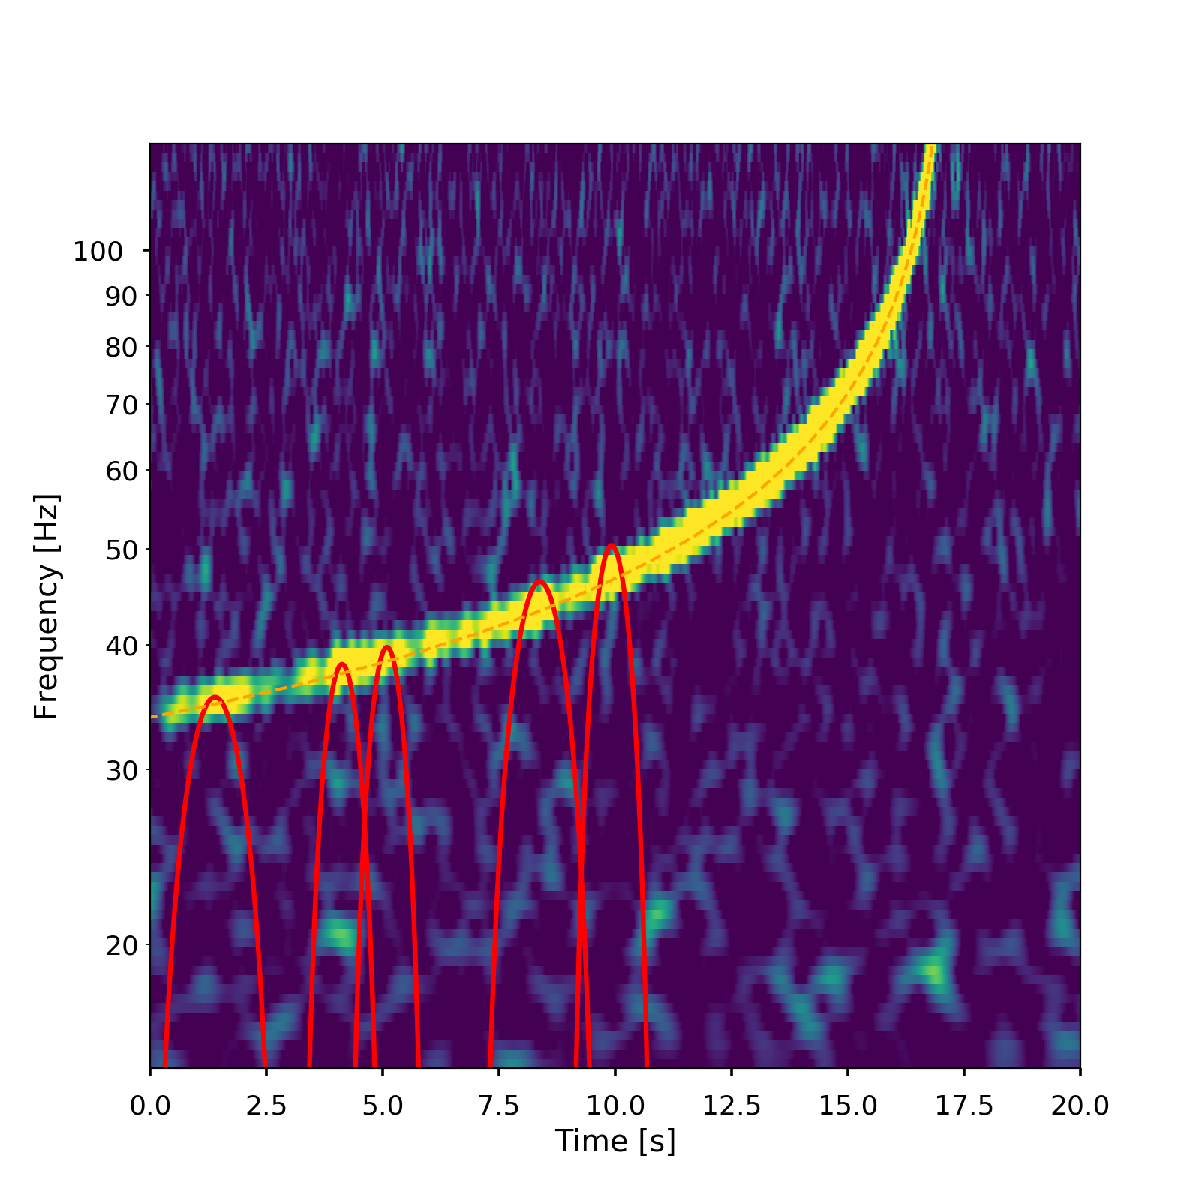
\includegraphics[width=0.49\linewidth]{images/4_archenemy/Section3/3.8/L1_loud_Original.pdf}
    \hspace{0.02\linewidth}
    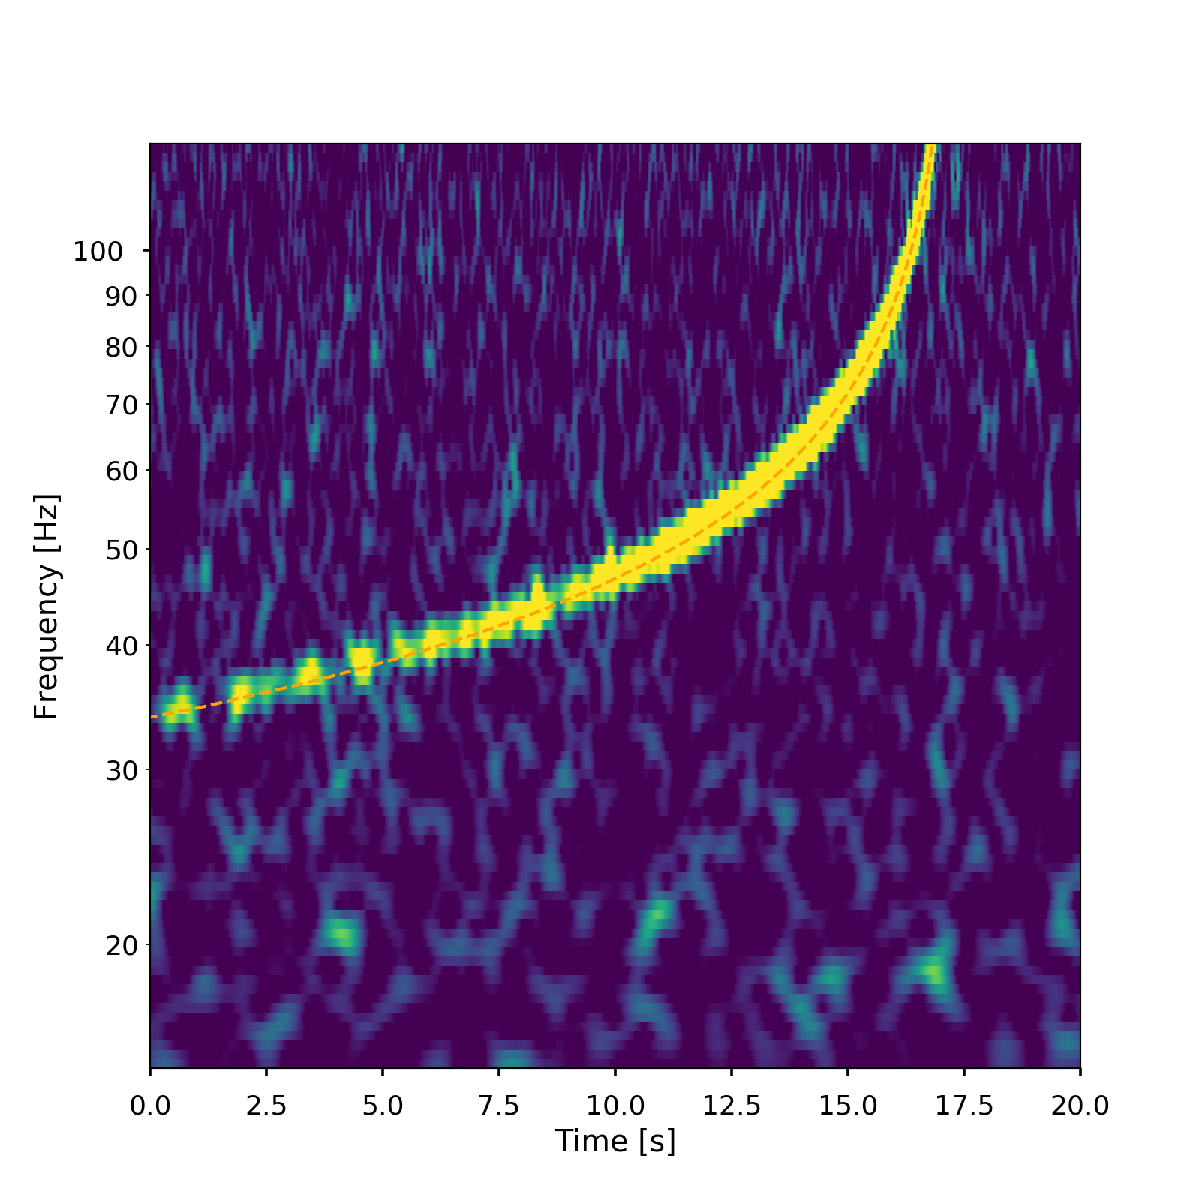
\includegraphics[width=0.49\linewidth]{images/4_archenemy/Section3/3.8/L1_loud_Subtracted.pdf}
  \end{minipage}
    \caption{An injected binary neutron star compact binary coalescence \gw{} signal, with the \scl{} glitches identified by the ArchEnemy search pipeline overlayed in red (left). The same injected signal but with the \scl{} glitches removed from the data (right). It can be seen that power is removed from the signal track and also there is an amount of power added to the data above the track.}
    \label{4:fig:loud_inj}
\end{figure}

\section{\label{4:sec:results}Assessing sensitivity gain from removing \scl{} glitches}

We now assess whether removing our identified list of \scl{} glitches results in a sensitivity gain when searching for compact binary mergers. We do this by comparing the results from the offline PyCBC search on the original data, to the results of the same search but analysing data where the glitches have been removed.

\subsection{Comparing search results with and without glitch subtraction}

The PyCBC pipeline is able to assess significance of potential compact binary mergers in a given stretch of data, and does the same with a set of simulated signals. This significance is quoted in terms of a ``false-alarm rate'', which denotes how often we would expect to see a non-astrophysical event at least as significant as the coincident trigger being considered. In this work we assess sensitivity at a false-alarm threshold of 2 background events every year.

The data we have searched over contained no previously found \gw{} signals~\cite{gwtc3:2023} and our search after subtracting \scl{} glitches identified no new \gw{} signals. While the search hasn't found any \gws{}, we can still measure the improvement in the sensitivity of the detectors by comparing the number of simulated signals identified with a false-alarm rate below 2 per year for each injection set (described in section~\ref{4:ssec:injsafety}) with and without removing glitches from the data. Table \ref{4:tab:found_injs} shows the number of injections found for all injection sets and both searches.
%
\begin{table}[tb]
\centering
\caption{\label{4:tab:found_injs}The number of injections found by each search with a false-alarm rate less than 2 per year alongside the number of newly-found and newly-missed injections, those found by the glitch-subtracted and not the original search and vice versa. We also show the sensitivity ratio of the glitch-subtracted search and original search for each injection set.} 
\footnotesize
\renewcommand{\arraystretch}{1.2}
\begin{tabular}{@{}cccccc}
\hline
Injection & Original  & Glitch- & Sensitivity & Newly & Newly \\
Type & Search & Subtracted & ratio & Found & Missed \\
\hline
BBH & 1215 & 1222 & 1.01 & 10 & 3 \\
BNS & 1315 & 1315 & 1.00 & 5 & 5 \\
NSBH & 1260 & 1265 & 1.00 & 8 & 3 \\
\hline
\end{tabular}


\end{table}

We compare the number of injections found by both searches but also look at the \gw{} injections found by the original search and missed by the glitch-subtracted search and vice versa, this information can be seen in table~\ref{4:tab:found_injs}. Considering signals found by the original search and missed by the glitch-subtracted search there are $3$ binary black hole injections with false-alarm rates in the original search ranging from $0.5\text{--}0.3$ per year, one of which had a glitch removed approximately $9$ seconds after the injection, there are $5$ newly-missed binary neutron star injections with false-alarm rates ranging from $0.5\text{--}0.056$ per year, two of the five binary neutron star injections had glitches removed within $60$ seconds of the injection, and there are $3$ newly-missed neutron star black hole injections with false-alarm rates ranging from $0.5\text{--}0.086$, one had glitches removed within $60$ seconds of the injection. The other newly-missed injections showed no \scl{} glitches within a $20$ second window for binary black hole injections and a $60$ second window for binary neutron star and neutron star black hole injections.

The glitch-subtracted search identifies $10$ additional binary black hole injections, the most significant of which have false-alarm rates of 1 per $190.50$, 1 per $7633.84$ and 1 per $8643.73$ years. We illustrate the last of these in figure~\ref{4:fig:ae_found} (top). $5$ extra binary neutron star injections were found, with false-alarm rates from $0.5\text{--}0.19$ per year and $8$ neutron star black hole injections were found, where the false-alarm rate of the most significant is 1 per $9961.55$ years. This injection can also be seen in figure~\ref{4:fig:ae_found} (bottom). We find $6$ of the $10$ binary black hole injections have \scl{} glitches within a $20$ second window of the injection, $3$ of $5$ binary neutron star injections have \scl{} glitches within a $60$ second window of the injection and, $6$ of the $8$ neutron star black hole injections have \scl{} glitches within a $60$ second window of the injection. We provide more details about the newly-found and newly-missed injections in~\ref{4:sec:apdx_injections_table}

\begin{figure}
  \centering
  \begin{minipage}[t]{1.0\linewidth}
    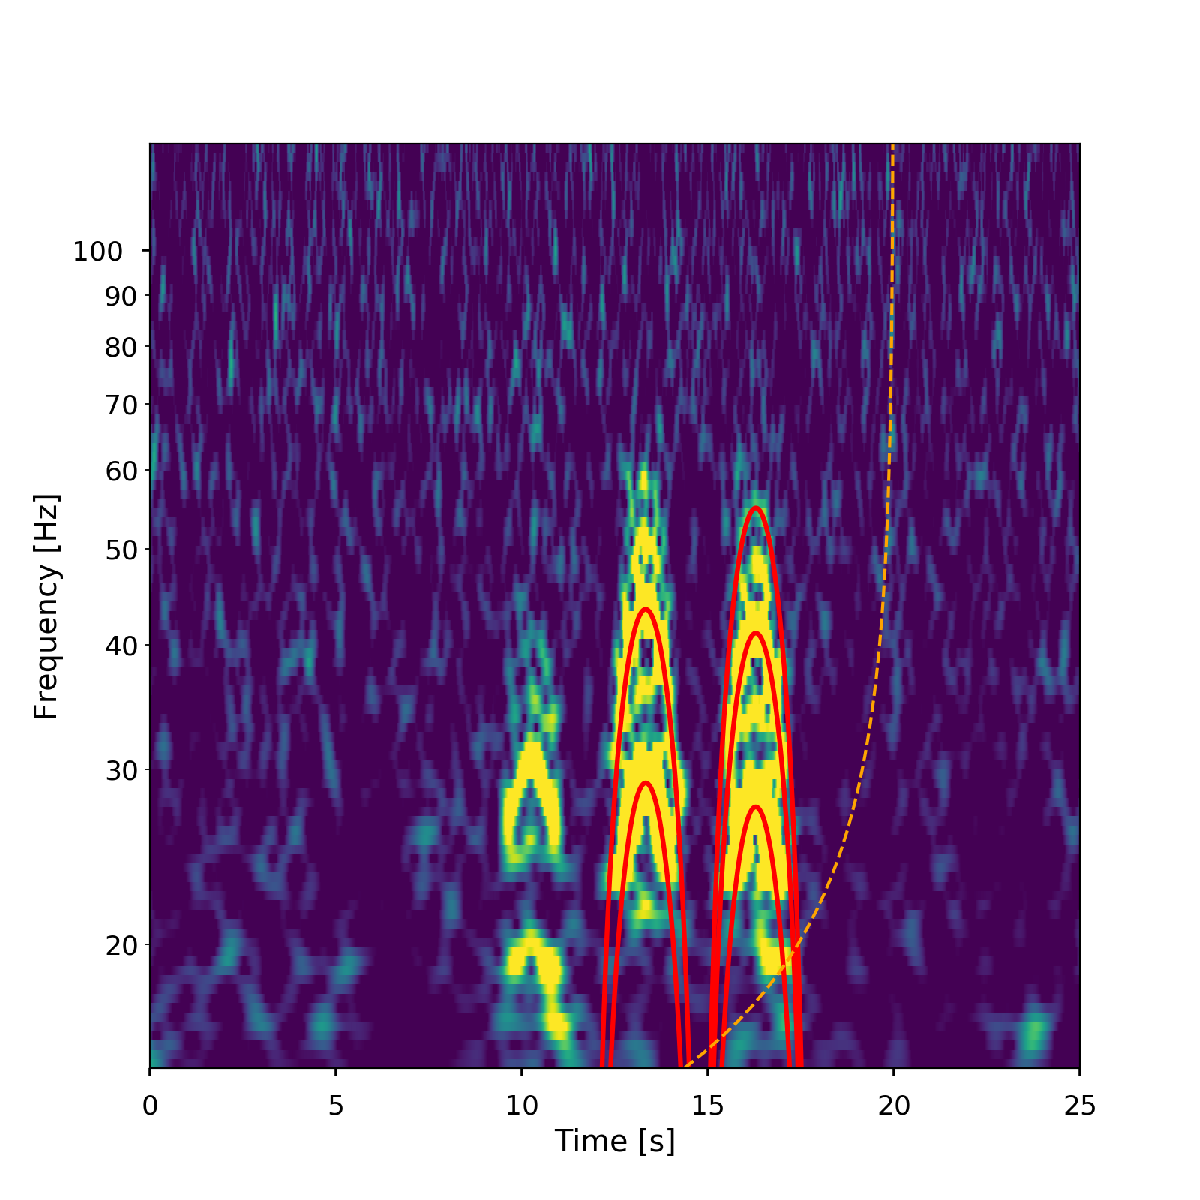
\includegraphics[width=0.49\linewidth]{images/4_archenemy/Section4/4.1/BBH_H1_loud_Original.pdf}
    \hspace{0.02\linewidth}
    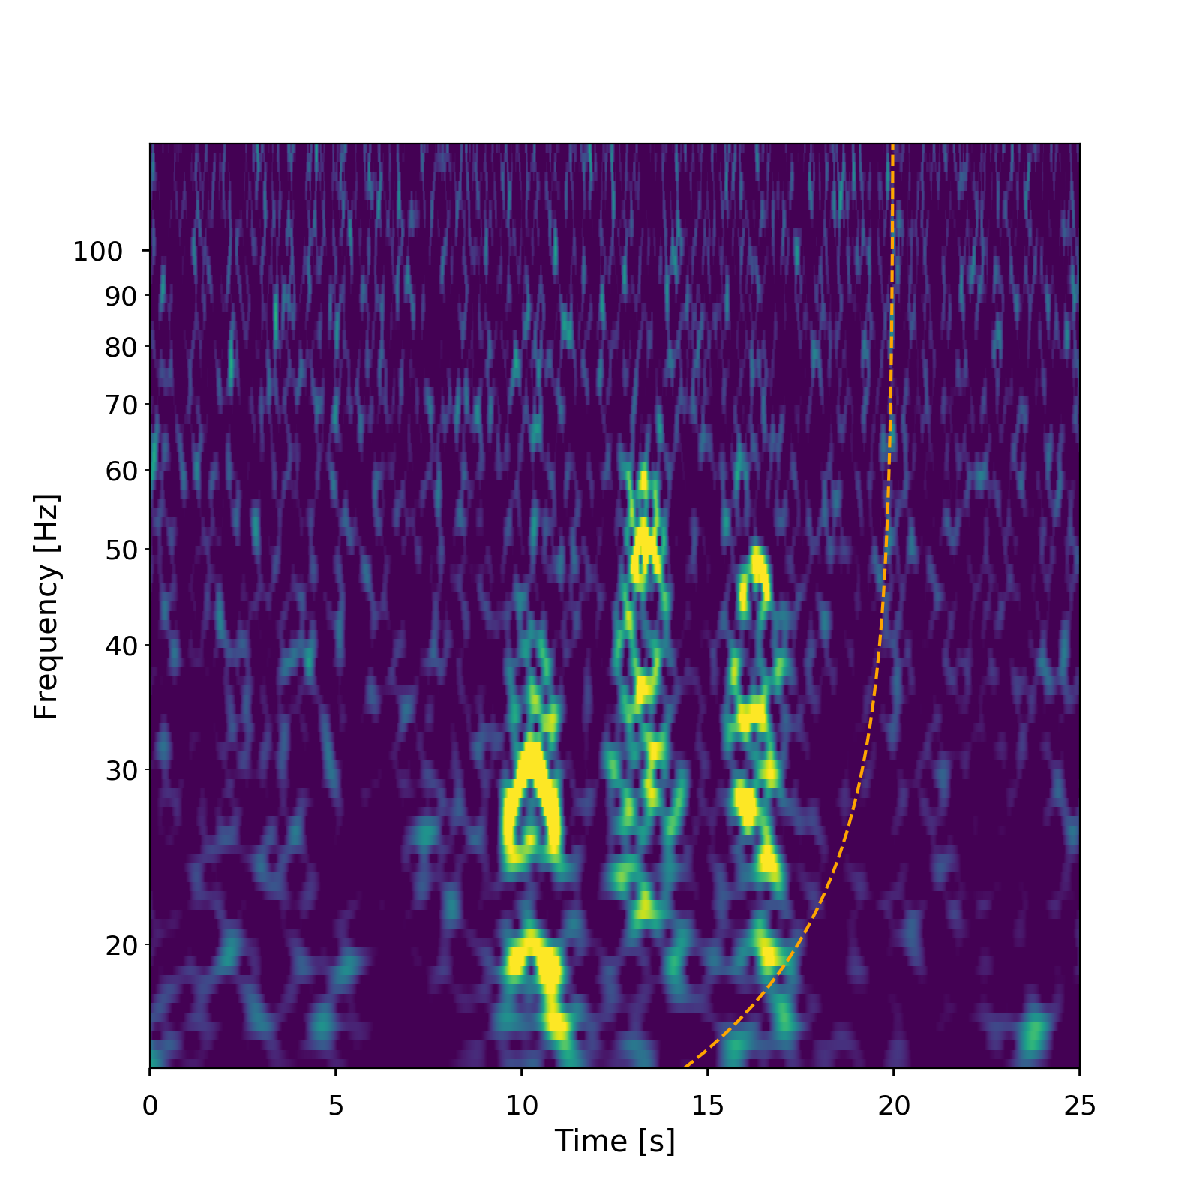
\includegraphics[width=0.49\linewidth]{images/4_archenemy/Section4/4.1/BBH_H1_loud_Subtracted.pdf}
  \end{minipage}
  \begin{minipage}[t]{1.0\linewidth}
    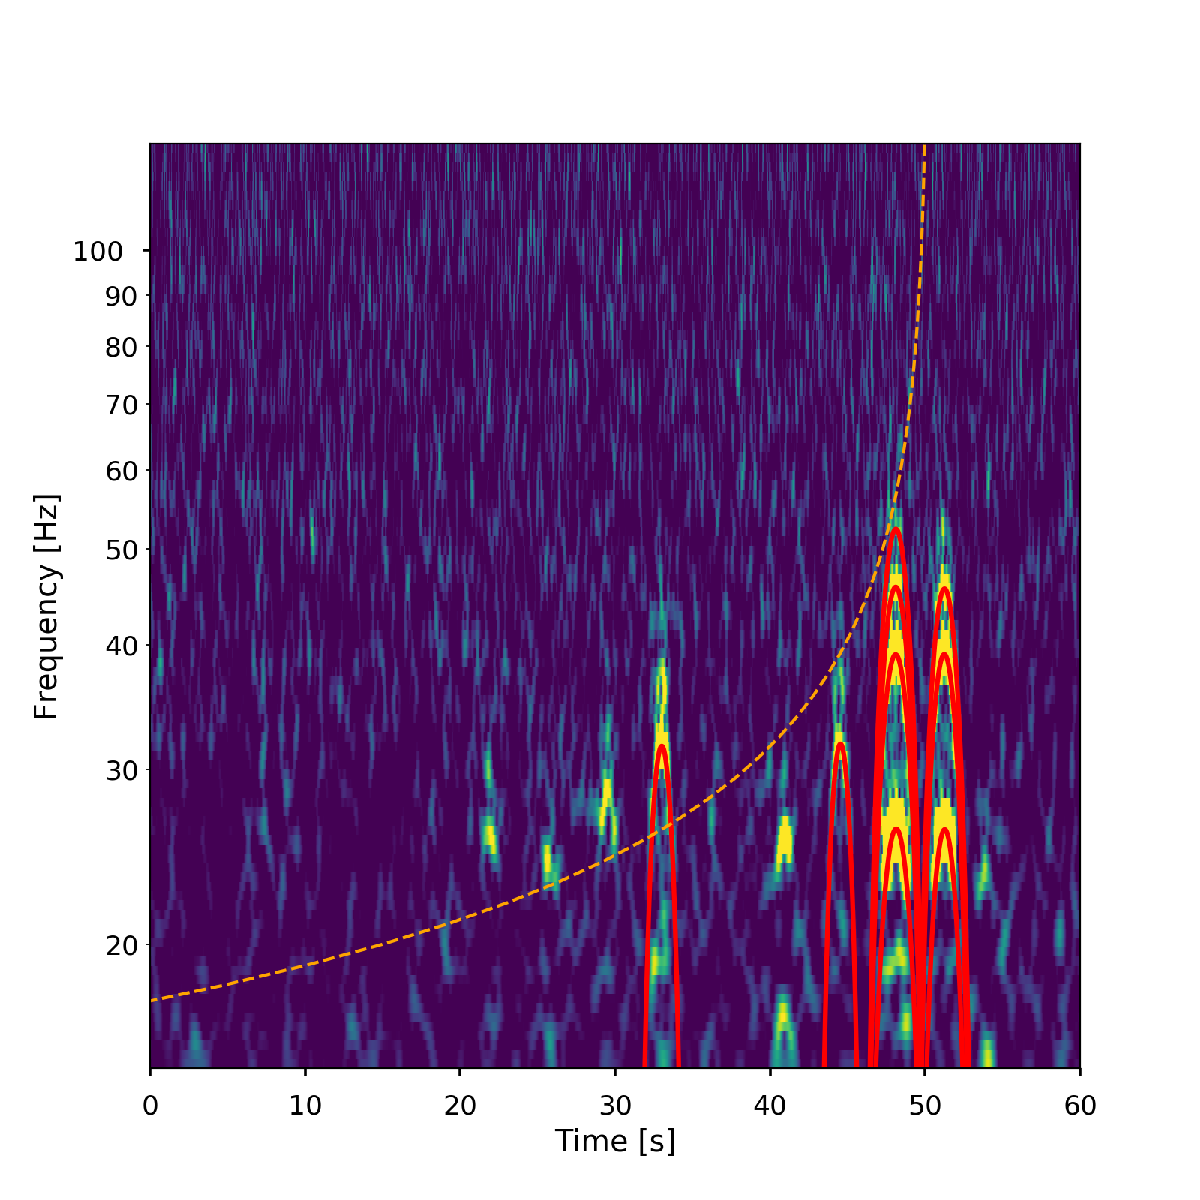
\includegraphics[width=0.49\linewidth]{images/4_archenemy/Section4/4.1/NSBH_H1_loud_Original.pdf}
    \hspace{0.02\linewidth}
    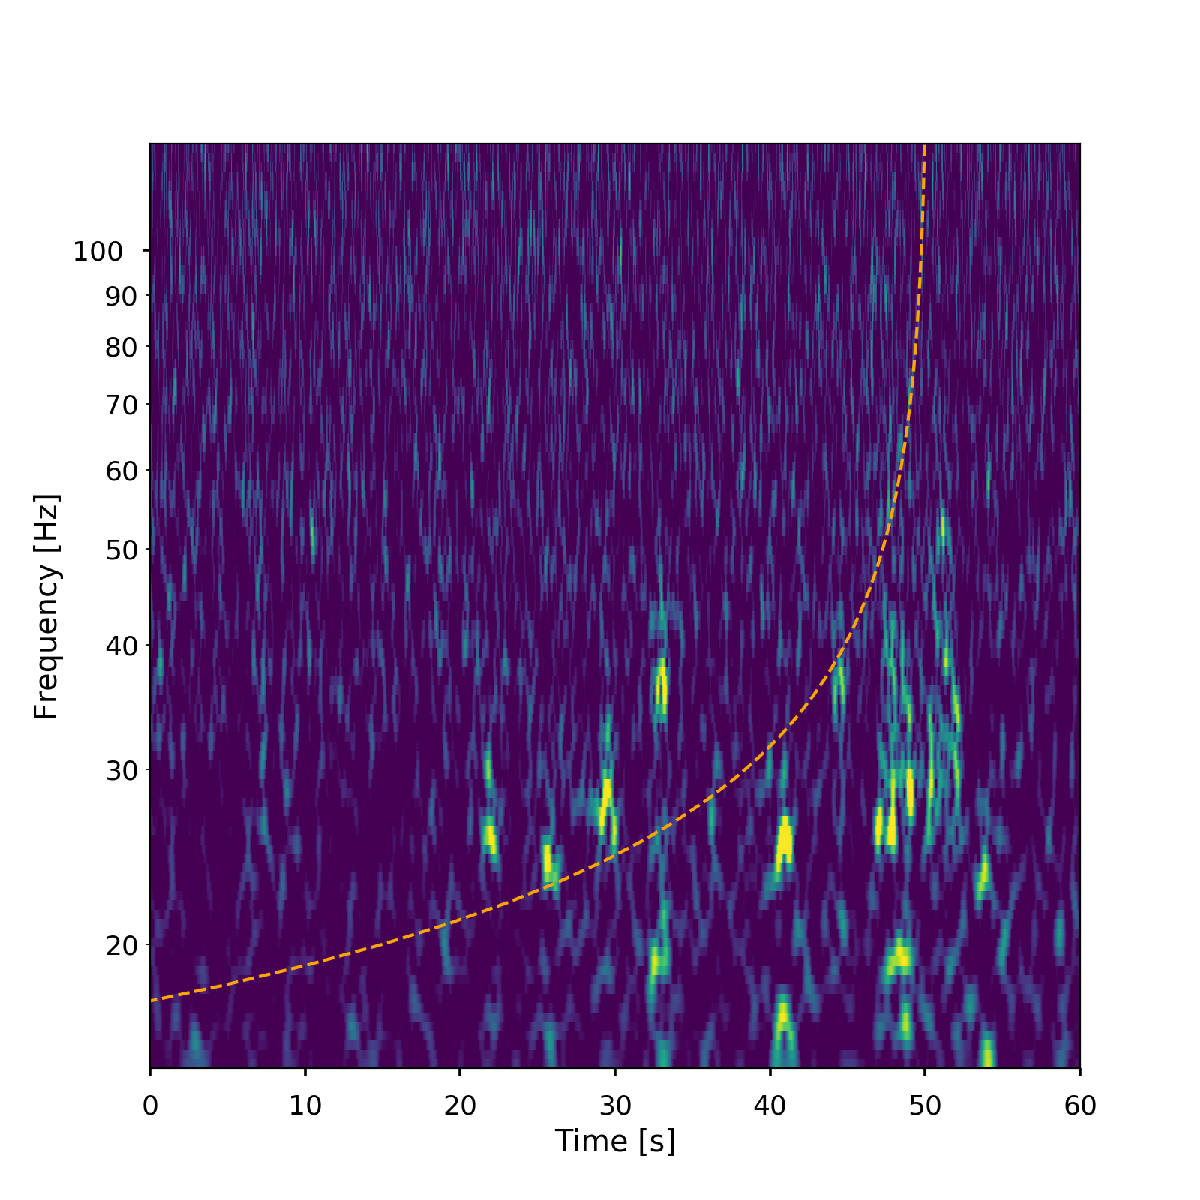
\includegraphics[width=0.49\linewidth]{images/4_archenemy/Section4/4.1/NSBH_H1_loud_Subtracted.pdf}
  \end{minipage}
    \caption{Two examples of \gw{} injections found by the glitch-subtracted search for \gws{} which were not found by the original \gw{} search due to the presence of \scl{} glitches at the same time as the \gw{} inspiral. Top left: A binary black hole injection with a false-alarm rate of 1 per $8643.73$ years is shown alongside the \scl{} glitches found by the ArchEnemy search and subtracted from the data prior to performing the glitch-subtracted PyCBC search for \gws{} (top right). Bottom left: A neutron star black hole injection with a false-alarm rate of 1 per $9961.55$ years and the \scl{} glitches found by the ArchEnemy search and subtracted from the data prior to performing the glitch-subtracted PyCBC search for \gws{} (bottom right).}
    \label{4:fig:ae_found}
\end{figure}

To quantify the sensitivity of the search we calculate the sensitive volume in which we can observe \gw{} signals. To calculate the sensitive volume we measure the detection efficiency of different distance bins taken from the injection sets and then multiply the efficiencies by the volume enclosed by the distance bins, these volumes are then summed to find the total volume the search is sensitive to~\cite{rw_snr_eq:2012}. We are then able to calculate the ratio in sensitivities between the glitch-subtracted \gw{} search and the original \gw{} search,  revealing the improvement that subtracting \scl{} glitches has made.

Figure~\ref{4:fig:allinj_vt_ratio} displays the ratio of the sensitive volume measured for the glitch-subtracted \gw{} search and the original PyCBC \gw{} search, across different false-alarm rate values, we quote our sensitivity ratios at a false-alarm rate value of 2 per year. The same set of injected signals was used for both \gw{} searches and therefore a direct comparison of search sensitivities can be made via this ratio. Disappointingly, the measured sensitivity improvement is small in the results we obtain. For the binary black hole injections we measure a sensitivity ratio at a 2 per year false-alarm rate of $1.01$, for binary neutron stars $1.00$ and neutron-star--black-holes $1.00$. 

The statistical significance of the sensitivity increase we report for the binary black hole injection set can be found by investigating the null hypothesis of seeing the same $1\%$ increase under the assumption that the subtraction of \scl{} glitches does not actually increase sensitivity. When performing this analysis we find that our result is not statistically significant at the 95\% confidence interval --i.e. there is a 5.24\% chance that we would measure such an increase in sensitivity at least as large as this under the null hypothesis-- (see~\ref{4:sec:apdx_stat_sig} for details). However, the marginal sensitivity increase would not justify repeating the \scl{} glitch search and glitch-subtracted \gw{} search on a larger injection set, instead more work is needed to better identify and remove \scl{} glitches while remaining safe in the presence of \gw{} signals.

\begin{figure}
     \centering
     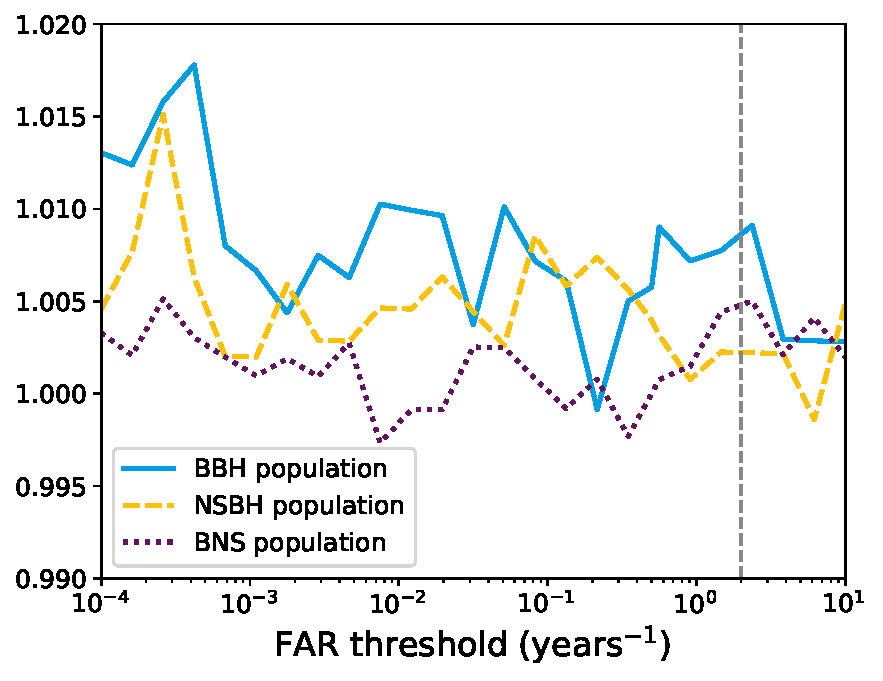
\includegraphics[width=0.7\textwidth]{images/4_archenemy/Section4/4.1/allinj_vt_ratio_ArchEnemy_coinc.pdf}
     \caption{The ratio of the sensitive volume-time of the glitch-subtracted search and the original \gw{} search. The grey dashed line indicates a false-alarm rate of $2$ per year which is our threshold and the point at which we measure any sensitivity improvements of the glitch-subtracted search for each of the three \gw{} injection sets. }
     \label{4:fig:allinj_vt_ratio}
\end{figure}

\section{\label{4:sec:conclusion}Conclusion}

We have demonstrated a new method for modelling \scl{} glitches and identifying and characterizing these glitches in a period of \gw{} data. We have developed a \scl{} glitch specific $\chi^{2}$ test which can discriminate between \scl{} glitches, other types of glitches and \gw{} signals. We have searched through a representative stretch of \gw{} data known to contain \scl{} glitches, found thousands of these glitches and subtracted them from the \gw{} data prior to running a search for \gws{}. The results of this search include a small increase in the measured sensitivity of the \gw{} search for binary black hole \gw{} signals, and modest change to sensitivity for binary neutron star and neutron star black hole \gw{} signals.

We highlight that the task of accurately identifying and parameterizing \scl{} glitches in the data is not a trivial one, especially where there are repeated, and harmonic, glitches present in the data. We have developed a new $\chi^{2}$ test to reduce the number of false identifications of \scl{} glitches, but we do still see cases where we have misidentified other glitches, and even a small number of loud \gw{} signals, as caused by \scl, and cases where we do not correctly identify, or parameterize, actual \scl{} glitches. Improving this identification process would be important in improving the efficacy of this process.

The possibility of using this model of \scl{} glitches as a bespoke application to \gw{} signals which are known to have coincident \scl{} glitches has been explored and implemented into Bilby~\cite{BILBY:2019} to perform a parameter estimation of \scl{} glitches and removing these to produce glitch-free data~\cite{Udall:2023}. The inclusion of the extra term from~\cite{Was_Subtract:2021} within the model can help identify \scl{} glitches more accurately. Selectively subtracting glitches based on the presence of a \gw{} signal is possible by moving the glitch subtraction process inside of the \gw{} searches and including the results of other \gw{} discriminators~\cite{rw_snr_eq:2012, McIsaac_Chi:2022} to determine the legitimacy of an ArchEnemy identified glitch.

The results of the application of the ArchEnemy search pipeline, the list of \scl{} glitches, can also be used in other applications. For example it could be used in the form of a veto~\cite{O2O3_DetChar:2021}, where we use knowledge of the presence of \scl{} glitches to down rank periods of time in \gw{} data. Additionally, we could use \scl{} glitches previously identified by tools such as Gravity Spy~\cite{gravityspy:2023} and target known \scl{} glitches with the ArchEnemy search pipeline.

As a final note, while we acknowledge that the sensitivity improvements that we have observed---${\sim} 1\%$---are very modest, the concept of removing \scl{} glitches, or other identified glitch classes, from the data prior to matched filtering for compact binary mergers is one that we encourage others to explore further. An increase in the rate of events or the rate of \scl{} glitches in future observing runs will mean an increase in the number of affected events, such techniques offer a method for mitigating the effect that these glitches will have on the search, maximizing the number of observations that can be made.
%
%%%%%%%%%%%%%%%%%%%%%%%%%%%%%%%%%%%%%%%%%%%%%%%%%%%%%%%%%%%%%%%%%%%%%%%%%%%%%%%%%%%%%%%%%%%%%%%%%%%
\section*{Appendix}
\section{\label{4:sec:apdx_stat_sig}Statistical significance}

We report a $1\%$ increase in the sensitivity for the binary black hole injection set in the glitch-subtracted \gw{} search (see section~\ref{4:sec:results}). We wish to determine the statistical significance of this result under the null hypothesis that subtracting \scl{} glitches prior to searching for \gws{} does not increase the sensitivity of the \gw{} search. The binary black hole injection set contains $6200$ injected signals, $10$ additional injections were found in the glitch-subtracted \gw{} search, $3$ additional injections were missed in our search, this gives us $13$ injections which have changed state.

First, we calculate the probability that an injection has been affected by the glitch removal, 
%
\begin{equation}
    p = \frac{13}{6200} = 0.21\% ,
\end{equation}
%
then we calculate the standard deviation, 
%
\begin{equation}
    \textrm{std} = \sqrt{n * p * (1 - p)} = 3.60 .
\end{equation}
%
Using the standard deviation we calculate the number of standard deviations our result deviates from the mean. We divide the number of positively changed (newly-found) injections by the standard deviation, 
%
\begin{equation}
    \textrm{standard deviations} = \frac{(10 - 3)}{3.60} = 1.94 .
\end{equation}
%
Under the assumption of no sensitivity increase caused by the subtraction of glitches, we measure our result of +7 newly-found \gw{} injections to lie $1.94$ standard deviations from an expected value of $0$ newly-found injections. The critical value of a 95\% confidence interval, that is to say there is a 1 in 20 chance of our null hypothesis being true, is $1.96$ meaning our result is within the 95\% confidence interval. We can describe this as there being a 5.24\% chance that our result is not caused by the subtraction of glitches but is instead caused by random chance. To reduce the error in the computed sensitivity ratio a larger injection set test would be required, this would need a large time and computational power investment which we do not believe is justified in the case of such a minor increase in the sensitivity.

\section{\label{4:sec:apdx_injections_table}Injections tables}

Here we have three tables which contain data on the newly-found and newly-missed injections for each injection set. The tables are separated into the values for the inverse false-alarm rate and ranking statistic found for each injection in both searches then the signal-to-noise ratio, $\chi^{2}$ and PSD variation values for each detector in both searches. The first table is the results of the binary black hole injection set, the second table is the binary neutron star injection set and the third is the neutron star black hole injection set. A horizontal dashed line separates newly-found and newly-missed injections, using a false-alarm rate threshold of 2 per year. There were 2 newly-found binary black hole injections which were not found at all by the original search and therefore they do not appear in the first table.

There have been 34 newly-found or newly-missed \gw{} injections when subtracting \scl{} glitches, it is informative to understand how the \gw{} search is influenced by the glitch subtraction to cause this outcome. The ranking statistic~\cite{PyCBC_global:2020} represents the legitimacy of a signal being astrophysical in origin and is partially computed using the re-weighted signal-to-noise ratio, which is itself computed using the initial signal-to-noise ratio alongside the various \gw{} discriminators and the PSD variation measurement~\cite{PSD_var:2020}. We use the trigger information saved by the \gw{} search to identify why injections that weren't found previously have been found post-glitch subtraction, and vice versa. 

As an example, we take the smallest false-alarm rate (1 per $8643.73$ years), newly-found, binary black hole injection, and look at the ranking statistic, signal-to-noise ratio, $\chi^{2}$ and, PSD variation measurements in both detectors and both searches -- these values can be found in table~\ref{4:tab:apdx_changed_snr_bbh}. This injection was originally seen with a false-alarm rate of 100 per year, far above our threshold, a very large increase in the ranking statistic from 13.29 to 27.01 is certainly responsible for the decreased false-alarm rate. There were no changes in the values measured by the LIGO-Livingston detector between searches which is expected as no \scl{} glitches were found within $512$ seconds of the injection. The LIGO-Hanford detector sees a small increase in the signal-to-noise ratio measured, from 7.98 to 8.22, a small increase in the $\chi^{2}$ value, from 2.32 to 2.48, and a very significant decrease in the PSD variation measurement, from 3.47 to 1.50. Using equation 18 of~\cite{PSD_var:2020}, we can calculate a re-weighted signal-to-noise ratio of $4.60$ for the original search and $5.67$ for the glitch-subtracted search, a significant increase in the signal-to-noise ratio. Similar analyses for all the newly-found and newly-missed injections can be made using information found in tables~\ref{4:tab:apdx_changed_snr_bns} and~\ref{4:tab:apdx_changed_snr_nsbh}.

The decrease in the PSD variation is true for the three newly-found very low false-alarm rate injections, accompanied by the small changes in signal-to-noise ratio and increase in the $\chi^{2}$ measurement. For newly-found and newly-missed injections which lie close to the 2 per year false-alarm rate threshold there is no definitive reason as to why these injections changed state.

\newpage
\newgeometry{left=2cm,right=2cm,top=2cm,bottom=2cm} % set new margins for one page
\begin{landscape}
\begin{table}[tb]
\centering
\caption{\label{4:tab:apdx_changed_snr_bbh}This table contains the trigger information for the newly-found and newly-missed \textbf{binary black hole injections} recorded by the original search~\cite{gwtc3:2023} and the glitch-subtracted search.} 
\begin{tabular}{|c|c|c|c|c|c|c|c||c|c|c|c|c|c|c|c|}
\hline
\multicolumn{8}{|c||}{Glitch-Subtracted} & \multicolumn{8}{c|}{Original Search} \\
\hline
\multicolumn{2}{|c|}{} & \multicolumn{3}{c|}{H1} & \multicolumn{3}{c||}{L1} & \multicolumn{2}{c|}{} & \multicolumn{3}{c|}{H1} & \multicolumn{3}{c|}{L1}\\
\hline
IFAR & Ranking & SNR & $\chi^{2}$ & PSD & SNR & $\chi^{2}$ & PSD & IFAR & Ranking & SNR & $\chi^{2}$ & PSD & SNR & $\chi^{2}$ & PSD \\ &

Stat. & & & Var. & & & Var. & & Stat. & & & Var. & & & Var.\\
\hline
8643.73 & 27.01 & 8.22 & 2.48 & 1.50 & 8.05 & 2.07 & 1.00 & 0.01 & 13.29 & 7.98 & 2.32 & 3.47 & 8.05 & 2.07 & 1.00 \\
7633.84 & 26.13 & 8.18 & 2.25 & 1.22 & 7.58 & 1.46 & 1.03 & 0.37 & 16.63 & 8.19 & 1.87 & 2.17 & 7.59 & 1.45 & 1.02 \\
4.89 & 19.06 & 7.23 & 1.88 & 0.97 & 10.34 & 3.15 & 1.05 & 1.56 & 18.01 & 7.24 & 2.11 & 0.97 & 10.34 & 3.42 & 1.04 \\
3.14 & 18.65 & 5.89 & 1.54 & 1.01 & 8.86 & 2.40 & 1.09 & 1.52 & 17.99 & 5.89 & 1.54 & 1.01 & 8.86 & 2.40 & 1.09 \\
2.75 & 18.53 & 8.50 & 1.63 & 0.99 & 6.80 & 1.37 & 1.05 & 1.51 & 17.98 & 8.51 & 1.56 & 0.98 & 6.80 & 1.37 & 1.05 \\
2.39 & 18.41 & 7.83 & 2.00 & 1.01 & 8.41 & 3.41 & 1.02 & 1.06 & 17.65 & 7.81 & 2.14 & 1.01 & 8.41 & 3.41 & 1.02 \\
2.18 & 18.32 & 7.02 & 1.90 & 1.02 & 6.35 & 2.15 & 1.01 & 1.79 & 18.14 & 7.05 & 1.92 & 1.02 & 6.35 & 2.16 & 1.01 \\
2.01 & 14.11 & 7.94 & 1.89 & 1.01 & 5.67 & 1.95 & 1.16 & 1.90 & 14.14 & 7.94 & 1.90 & 1.01 & 5.07 & 0.00 & 1.02 \\
\hdashline
1.76 & 18.12 & 6.89 & 1.43 & 1.02 & 6.76 & 2.59 & 0.97 & 3.33 & 18.71 & 6.86 & 1.82 & 1.02 & 6.68 & 2.53 & 0.97 \\
1.79 & 18.14 & 6.40 & 1.69 & 1.02 & 7.56 & 2.01 & 1.01 & 2.05 & 18.27 & 6.40 & 1.69 & 1.02 & 7.56 & 2.00 & 1.01 \\
1.65 & 18.06 & 5.14 & 0.00 & 0.91 & 7.57 & 1.57 & 1.02 & 2.05 & 18.27 & 5.14 & 0.00 & 0.91 & 7.57 & 1.57 & 1.02 \\
\hline
\end{tabular}
\end{table}
\end{landscape}
\restoregeometry % restore the default margins for subsequent pages

\newpage

\newgeometry{left=1cm,right=1cm,top=2cm,bottom=2cm} % set new margins for one page
\begin{landscape}
\begin{table}[tb]
\centering
\caption{\label{4:tab:apdx_changed_snr_bns}This table contains the trigger information for the newly-found and newly-missed \textbf{binary neutron star injections} recorded by the original search~\cite{gwtc3:2023} and the glitch-subtracted search.} 
\begin{tabular}{|c|c|c|c|c|c|c|c||c|c|c|c|c|c|c|c|}
\hline
\multicolumn{8}{|c||}{Glitch-Subtracted} & \multicolumn{8}{c|}{Original Search} \\
\hline
\multicolumn{2}{|c|}{} & \multicolumn{3}{c|}{H1} & \multicolumn{3}{c||}{L1} & \multicolumn{2}{c|}{} & \multicolumn{3}{c|}{H1} & \multicolumn{3}{c|}{L1}\\
\hline
IFAR & Ranking & SNR & $\chi^{2}$ & PSD & SNR & $\chi^{2}$ & PSD & IFAR & Ranking & SNR & $\chi^{2}$ & PSD & SNR & $\chi^{2}$ & PSD \\ &
Stat. & & & Var. & & & Var. & & Stat. & & & Var. & & & Var.\\
\hline
5.12 & 19.12 & 5.86 & 1.99 & 1.01 & 7.15 & 1.94 & 1.02 & 1.49 & 17.96 & 5.74 & 2.14 & 1.01 & 7.15 & 1.94 & 1.02 \\
4.91 & 19.07 & 5.48 & 2.29 & 1.01 & 7.92 & 2.16 & 1.01 & 1.37 & 17.89 & 5.78 & 2.25 & 1.01 & 7.23 & 2.13 & 1.01 \\
4.54 & 18.99 & 4.82 & 0.00 & 1.07 & 8.68 & 2.05 & 1.06 & 1.66 & 18.07 & 4.82 & 0.00 & 1.14 & 8.68 & 2.05 & 1.06 \\
2.46 & 18.43 & 5.48 & 1.95 & 1.05 & 7.61 & 2.03 & 0.99 & 1.78 & 18.13 & 5.48 & 1.94 & 1.05 & 7.62 & 2.08 & 0.99 \\
2.34 & 18.39 & 6.25 & 2.18 & 1.01 & 6.82 & 1.96 & 1.00 & 1.45 & 17.94 & 6.09 & 2.05 & 1.01 & 6.83 & 2.01 & 1.00 \\
\hdashline
1.24 & 17.71 & 6.58 & 2.14 & 1.01 & 6.89 & 2.48 & 1.01 & 17.81 & 20.19 & 6.58 & 2.15 & 1.01 & 7.16 & 2.26 & 1.01 \\
1.14 & 17.72 & 6.00 & 2.67 & 0.98 & 8.07 & 2.66 & 1.22 & 7.14 & 19.44 & 6.17 & 2.45 & 0.97 & 8.26 & 2.80 & 1.22 \\
1.89 & 18.19 & 6.32 & 2.19 & 1.00 & 6.79 & 1.83 & 0.99 & 3.57 & 18.78 & 6.37 & 2.12 & 0.99 & 6.79 & 1.75 & 0.99 \\
0.88 & 17.46 & 6.88 & 2.14 & 0.99 & 6.19 & 2.12 & 0.99 & 2.33 & 18.39 & 6.87 & 2.07 & 0.99 & 6.19 & 1.99 & 0.99 \\
1.36 & 17.80 & 6.20 & 2.02 & 1.00 & 6.83 & 2.35 & 1.00 & 2.07 & 18.18 & 6.20 & 2.02 & 1.00 & 6.83 & 2.28 & 1.00 \\
\hline
\end{tabular}
\end{table}
\end{landscape}
\restoregeometry % restore the default margins for subsequent pages

\newpage

\newgeometry{left=1cm,right=1cm,top=2cm,bottom=2cm} % set new margins for one page
\begin{landscape}
\begin{table}[tb]
\centering
\caption{\label{4:tab:apdx_changed_snr_nsbh}This table contains the trigger information for the newly-found and newly-missed \textbf{neutron star black hole injections} recorded by the original search~\cite{gwtc3:2023} and the glitch-subtracted search.} 
\begin{tabular}{|c|c|c|c|c|c|c|c||c|c|c|c|c|c|c|c|}
\hline
\multicolumn{8}{|c||}{Glitch-Subtracted} & \multicolumn{8}{c|}{Original Search} \\
\hline
\multicolumn{2}{|c|}{} & \multicolumn{3}{c|}{H1} & \multicolumn{3}{c||}{L1} & \multicolumn{2}{c|}{} & \multicolumn{3}{c|}{H1} & \multicolumn{3}{c|}{L1}\\
\hline
IFAR & Ranking & SNR & $\chi^{2}$ & PSD & SNR & $\chi^{2}$ & PSD & IFAR & Ranking & SNR & $\chi^{2}$ & PSD & SNR & $\chi^{2}$ & PSD \\ &
Stat. & & & Var. & & & Var. & & Stat. & & & Var. & & & Var.\\
\hline
9961.55 & 27.41 & 5.55 & 2.08 & 1.23 & 10.26 & 2.27 & 1.12 & 0.01 & 12.83 & 6.01 & 2.39 & 2.25 & 8.54 & 2.37 & 1.12 \\
141.35 & 22.28 & 7.76 & 2.20 & 1.02 & 6.54 & 2.35 & 1.01 & 1.21 & 17.77 & 7.83 & 1.94 & 1.02 & 7.29 & 2.50 & 1.00 \\
18.26 & 20.36 & 5.94 & 2.20 & 1.09 & 6.02 & 1.99 & 1.10 & 1.29 & 17.82 & 5.74 & 2.05 & 1.09 & 6.27 & 2.10 & 1.18 \\
17.12 & 20.29 & 7.64 & 2.00 & 1.11 & 6.66 & 2.15 & 1.05 & 1.37 & 17.89 & 7.36 & 2.35 & 1.11 & 6.66 & 2.15 & 1.05 \\
12.94 & 20.03 & 6.52 & 1.79 & 1.07 & 7.31 & 2.32 & 1.13 & 1.96 & 18.23 & 6.57 & 1.85 & 1.20 & 7.31 & 2.32 & 1.13 \\
7.12 & 19.42 & 5.13 & 0.00 & 1.05 & 8.33 & 2.08 & 1.04 & 0.03 & 14.23 & 5.30 & 2.16 & 1.05 & 7.44 & 2.43 & 1.04 \\
3.61 & 18.77 & 5.80 & 2.01 & 1.02 & 7.43 & 1.88 & 0.93 & 1.81 & 18.15 & 5.80 & 2.01 & 1.02 & 7.43 & 1.97 & 0.93 \\
2.15 & 18.22 & 7.41 & 2.04 & 1.02 & 5.57 & 2.03 & 1.03 & 0.00 & 4.34 & 5.64 & 2.18 & 0.98 & 5.04 & -0.00 & 1.01 \\
\hdashline
0.23 & 16.16 & 5.79 & 1.81 & 0.96 & 8.78 & 3.93 & 1.03 & 11.69 & 19.93 & 5.78 & 1.89 & 0.96 & 8.79 & 3.17 & 1.03 \\
1.56 & 17.92 & 6.71 & 1.91 & 0.99 & 6.73 & 2.50 & 1.05 & 2.68 & 18.41 & 6.71 & 1.90 & 0.99 & 6.72 & 2.39 & 1.05 \\
1.72 & 18.10 & 5.77 & 1.90 & 0.99 & 6.77 & 1.74 & 1.00 & 2.08 & 18.28 & 5.77 & 1.90 & 0.99 & 6.80 & 1.69 & 1.00 \\
\hline
\end{tabular}
\end{table}
\end{landscape}
\restoregeometry % restore the default margins for subsequent pages

%%begin novalidate


%---% PyCBC Live Ranking Statistic %---%
\chapter[Improving the PyCBC Live Ranking Statistic]{\label{chapter:5-pycbc-live}Improving the PyCBC Live Ranking Statistic}
\chapterquote{``This chapter needs a quote'' - Arthur Tolley}
The project described in this chapter required making significant changes to the PyCBC Live search. The changes to the PyCBC Live ranking statistic code were made by myself however, to use these changes in the PyCBC Live search another significant set of changes were required to implement the structural code that defines how PyCBC Live runs on the supercomputer infrastructure. Therefore, this work has not currently been published, it is aimed to form part of the PyCBC Live fourth observing run methods paper which is currently being written. Significant contributions were made by Gareth Cabourn Davies and Max Trevor to enable these changes to be run in the second half of the fourth observing run.

\section{\label{5:sec:introduction}Introduction}

Searching for gravitational waves is done using search pipelines. The search pipelines exist across two timelines: low-latency, rapid detection of gravitational wave signals in real-time; and offline, which is performed months after the data has been obtained. Low-latency search pipelines are optimised for rapid detection to disseminate information about potential gravitational wave signals to the wider scientific community in as little time as possible, the latency between a gravitational wave signal arriving at the detectors and being detected by search pipelines is crucial for multi-messenger events.

There were a number of gravitational wave search pipelines operational in offline during the third observing run: cWB~\cite{cWB:2020}, GstLAL~\cite{GstLAL:2020}, MBTA~\cite{MBTA:2021} and PyCBC Offline~\cite{PyCBC_global:2020}. Table XIV in Appendix D 7a of the second half of the third observing run's catalogue paper~\cite{gwtc3:2023} highlights that the PyCBC Offline search is the most sensitive gravitational wave search pipeline~\cite{PyCBC:2016, PyCBC:2017, PyCBC_package:2021}.

The low-latency gravitational wave search pipelines include: cWB~\cite{cWB:2020}, GstLAL~\cite{GstLAL:2020}, MBTA~\cite{MBTA:2021}, PyCBC Live~\cite{PyCBC_Live:2018}, SPIIR~\cite{SPIIR:2020} and, oLIB~\cite{oLIB:2015}. The PyCBC live search pipeline is not the most sensitive in the low-latency regime. In the third and first half of the fourth observing runs the GstLAL pipeline~\cite{GstLAL:2020} 
%% COUNT THE NUMBER OF EVENTS FOUND INSTEAD OF THE PREFERRED EVENTS %%
was the preferred event for X of the Y low-latency events whereas PyCBC live was only preferred in Z events. We want to improve the PyCBC live search to have the same sensitivity as its offline counterpart and to do this we must look at the key differences between the two searches.

Offline searches for gravitational waves are capable of using post-detection information when processing their results and have no limit on the amount of computational analysis that can be done to find events. Low-latency gravitational wave searches, such as PyCBC Live, receive and analyse data in regular fixed analysis segments and all computational processing must be completed before the next analysis segment arrives. If the triggers in an analysis segment are not processed in time, then lag is introduced as a backlog of triggers builds up faster than they can be processed. The maximum latency between an event arriving and being detected by PyCBC Live during the third observing run was $20$ seconds~\cite{PyCBC:2017}. The latency restriction of the PyCBC Live search prevents PyCBC Live from using post-detection information in its event detection.

PyCBC Offline contains new components and information that can be used by the PyCBC Live search without violating the latency restrictions. Introducing these new components into the live search will improve the sensitivity of the gravitational wave search, bringing the two PyCBC searches closer to parity and detecting more gravitational wave events with greater significance.

This chapter is laid out as follows: in section blah blah blah.

\section{\label{5:sec:ranking-stat}The Ranking Statistic}

% what is a ranking statistic
The ranking statistic produces a post-detection quantification of the legitimacy of a gravitational wave detection. The ranking statistic values can be mapped directly to false-alarm rate (FAR), a key metric used to assess the likelihood that a detected signal is real and not a result of coincident noise triggers being found by the gravitational wave search~\cite{PyCBC_global:2020}.

% What does it do
A ranking statistic combines numerous pieces of information about a candidate event to provide a single measure that reflects the event's significance. The ranking statistic can include information such as: single detector trigger signal-to-noise ratio, $\rho$, signal-consistency tests~\cite{Allen_Chi:2005, rw_snr_eq:2012, PyCBC_sg:2018} and, coincidence tests between detectors. It can also include more complex information like coincident phase and time difference likelihood based on source localisation and detector orientation~\cite{PyCBC:2017, PyCBC_singles:2022}. Different ranking statistics combine different pieces of information to make the final assessment of significance.

% A good description of the effects of having one
Improving the ranking statistic used in the PyCBC Live search will improve the search's ability to distinguish between real gravitational wave events and false-alarms. The PyCBC Offline search's ranking statistic contains more information than the ranking statistic used by PyCBC Live during the third observing run, some of which we can adapt for the PyCBC Live search~\cite{PSD_var:2020, PyCBC:2017, PyCBC_global:2020}.

\section{\label{5:sec:previous-stat}PyCBC Ranking Statistics Used in O3}

% How does a ranking statistic work: single first then coincident
In PyCBC searches the ranking statistic first calculates the single detector ranking statistic for each online detector. The single detector ranking statistic from each detector is then combined and coincidences are formed between triggers to identify potential gravitational wave events. The coincident triggers are then ranked by the coincident ranking statistic to provide the final ranking statistic value. 

% The PyCBC Offline third observing run ranking statistic
The PyCBC Offline search in the third observing run ranked single detector triggers by: signal-to-noise ratio, $\rho$, calculated by the matched filter of template and data~\cite{FINDCHIRP:2012}; the traditional $\chi^{2}$, calculated by measuring the difference in the expected and actual $\rho$ for discrete frequency bins in the signal evolution~\cite{Allen_Chi:2005}; the sine-gaussian $\chi^{2}$, which measures $\rho$ in frequency bins above the signal's maximum frequency~\cite{PyCBC_sg:2018} and; PSD variation, which estimates the effect of non-stationary noise on $\rho$, re-weighting $\rho$ prior to applying the $\chi^{2}$ tests~\cite{PSD_var:2020}. These four single detector ranking statistic components are applied to all triggers found by the search to give a new re-weighted $\rho$ value, $\hat{\rho}$~\cite{rw_snr_eq:2012}. \cite{McIsaac_Chi:2022} provides a detailed review of the $\chi^{2}$ tests currently being used in gravitational wave searches.

After the calculation of $\hat{\rho}$ for each single detector trigger, the different detector triggers are combined and a coincidence test is applied to identify coincident triggers. The coincidence test checks whether the arrival time of the gravitational wave signal at the separate detectors is possible given the light-travel time of the gravitational wave signal, for example, the two LIGO detectors are separated by a straight line through the Earth $3002$ kilometers long. Given the speed of light, c $= 300,000$ km/s, there is a $0.01$ second maximum physical travel time for a signal detected by one detector to appear in the other detector. On top of this time window, we add an additional $0.02$ seconds to account for computational timing differences between the two detectors, giving a total allowed time difference between trigger arrival times at different detectors of $0.03$ seconds.

Triggers across detectors found within the time window and above the $\hat{\rho}$ threshold (typically $4.5$) can be considered coincident and are passed to the coincident ranking statistic for ranking. The PyCBC Offline coincident ranking statistic includes: likelihood of coincident trigger time and phase differences~\cite{PyCBC:2016}, likelihood correction based on data artefacts found in correlated auxiliary channels which are insensitive to gravitational waves~\cite{DQ_vetoes:2017, iDQ:2020}, an exponential noise model which models noise distributions of templates separately and re-ranks single detector ranking statistic based on how frequently a template has historically triggered on noise with high $\hat{\rho}$~\cite{PyCBC:2017}, and a template dependent factor which re-weights templates based on their astrophysical likelihood~\cite{PyCBC_focussed_bbh:2024}.

% The PyCBC Live third observing run ranking statistic
The PyCBC Live ranking statistic used during the third observing run was comparatively simple. The single detector ranking statistic is the same as the PyCBC Offline single detector ranking statistic except without the PSD variation statistic. PyCBC Live only ranks coincident triggers by the likelihood of their time and phase differences~\cite{PyCBC_Live:2018}.

\subsection{\label{5:sec:old-stat-construction}Constructing the O3 PyCBC Live Ranking Statistic}

We describe the ranking statistic used by PyCBC Live during the third observing run in more detail to identify the potential components that can be added from the PyCBC Offline ranking statistic. The construction of the ranking statistic used by PyCBC Live during the third observing run is described in~\cite{PyCBC_Live:2018}. Using approximations of the signal event rate density (signal rate), $p^{S}(\Vec{\theta})$, and noise event rate density (noise rate), $p^{N}(\Vec{\theta})$, over the parameter space $\Vec{\theta} = \left(\hat{\rho}_{H}, \hat{\rho}_{L}, \chi^{2}_{H}, \chi^{2}_{L}, \delta\phi, \delta t, m_{1}, m_{2}, \Vec{s_{1}}, \Vec{s_{2}}\right)$ we can form a general detection statistic from the ratio of the densities,
%
\begin{equation}
    R^{2} \propto 2 [\log p^{S}(\Vec{\theta}) - \log p^{N}(\Vec{\theta})] + constant.
    \label{5:eqn:general-detection-statistic}
\end{equation}
%
This construction is chosen such that the ranking statistic of a two detector coincidence with both Gaussian and stationary noise~\footnote{The detector noise is \textbf{not} assumed to be Gaussian and stationary but this ranking statistic is recovered if that were the case.} will have single detector noise rate that falls off as a Gaussian,
%
\begin{equation}
    r_{n,det} \propto \exp \left( -\frac{(\rho_d - \mu)^2}{2 \sigma^2} \right) ,
    \label{5:eqn:old-noise-rate}
\end{equation}
%
so the combined detector noise rate is the product of both detector noise rates,
%
\begin{equation}
    p^{N}(\Vec{\theta}) \propto \exp \left( -\frac{(\rho_{H}^{2} + \rho_{L}^{2})}{2} \right) ,
    \label{5:eqn:old-comb-noise-rate}
\end{equation}
%
and the standard quadrature sum signal-to-noise ratio statistic is recovered,
%
\begin{equation}
    R^{2} = -2 \log p^{N}(\Vec{\theta}) = \rho^{2}_{H} + \rho^{2}_{L} .
\end{equation}

To expand on the quadrature sum ranking statistic, which only considers the noise rate, we can include information about the signal rate which takes the parameters $(\rho_{H}, \rho_{L}, \delta t, \delta \phi)$: the two detector signal-to-noise ratios, the difference in the time of arrival for the two detectors, $\delta t = t_{H} - t_{L}$, and the difference in phase of the gravitational waveforms, $\delta \phi = \phi_{H} - \phi_{L}$. These parameters, for a real signal, will depend on the source localisation and detector orientation and therefore, some combinations of parameters are more likely than others. The exact process for calculating $p^{S}(\Vec{\theta})$ is provided in detail in~\cite{PyCBC:2017}, for this chapter's purpose a look-up is made to a phase-time histogram which represents the most likely combination of the two parameters in the signal space. Including $p^{S}(\Vec{\theta})$ in the general ranking statistic (equation~\ref{5:eqn:general-detection-statistic}) yields,
%
\begin{equation}
    R = \sqrt{\rho^{2}_{H} + \rho^{2}_{L} + 2 \log\left(p^{S}(\Vec{\theta})\right)}
    \label{5:eqn:original-statistic}
\end{equation}
%
which is the final version of the original ranking statistic used by PyCBC Live in the third observing run.

\section{\label{5:new-additions}Adding to the PyCBC Live Ranking Statistic}

The ranking statistic used by PyCBC Live in the third observing run combines the noise rate contribution, which is the quadrature sum of detector $\hat{\rho}$ in stationary, Gaussian noise, and the signal rate of the trigger. We know our detector noise is \textbf{not} stationary and Gaussian~\cite{LIGO_data_quality:2015} and therefore by including an accurate noise model in the ranking statistic we can improve the sensitivity of the PyCBC Live search.

There are two components of the PyCBC Offline ranking statistic that directly address these two deficiencies in our ranking statistic: PSD variation, which corrects the single detector $\rho$ for non-stationary noise present in the data and; the exponential noise model, which models the noise distribution of each template by fitting an exponential to the noise falloff.

The other components of the PyCBC Offline ranking statistic that we haven't chosen to include are in development in parallel to our changes and can be included in the PyCBC Live ranking statistic in the future.

\subsection{\label{5:sec:psd-var}PSD Variation}

% Motivation
Non-stationary noise is that which originates from instrumental noise such as seismic noise, thermal noise and quantum noise and cannot be mitigated except through detector improvements. The power spectral density (PSD) describes how much power is present in the data at each frequency, essentially how the data power is distributed in the frequency domain. Non-stationary noise will change the noise profile over the period of the search segment, meaning the PSD will be inaccurate at different times. 

Identifying triggers in the PyCBC searches is done by matched filtering the data with a signal template,
%
\begin{equation}
  \rho(t) = \frac{(h | s)}{\sqrt{(h | h)}} \equiv (\hat{h} | s),
  \label{5:eqn:mf_1}
\end{equation}
%
here $h$ is the model template, $s$ the gravitational wave data we are searching and we use the noise-weighted inner product defined between two time series $a(t)$ and $b(t)$ as
%
\begin{equation}
  (a | b) = 4 Re \int^{\infty}_{0} \frac{\tilde{a}(f) \tilde{b}^*(f)}{S_n(f)} 
  %e^{-2 \pi i f t} 
  df.
  \label{5:eqn:inner_product}
\end{equation}
%
The tilde on $\tilde{a}$ and $\tilde{b}$ refer to the Fourier-transform of both variables into the frequency domain and $S_n(f)$ is the one-sided PSD of the data is defined as
%
\begin{equation}
  \langle \tilde{s}(f) \tilde{s}(f^\prime) \rangle = \frac{1}{2} S_n(f) \delta(f - f^\prime) \;,
  \label{5:eqn:psd}
\end{equation}
%
where the angle brackets denote an average over noise realisations and $\delta$ is the Dirac delta function. A PSD which doesn't accurately describe the noise profile of the data will lead to a miss-estimation in the calculation of $\rho$. The offline search empirically measures the PSD of the gravitational wave data being analysed using Welch's method, however, instead of using a mean average of the overlapping PSDs a median average it used to remove the effect of short duration glitches in the data.

% What is the problem of non-stationary noise
The estimated PSD is used for very long search segments ($512$ seconds) and while the effects of short duration glitches have been mitigated with the median average method we still suffer from the effects of non-stationary noise. 

% What is PSD Variation
The mismatch between the estimated PSD, $S_{E}$, and actual PSD, $S_{A}$, of the data will have the effect of underestimating and overestimating the noise at different times in our search segment. We are able to track the sources of the non-stationary noise in some cases, for example, when the source of the non-stationary noise is a period of increased seismic activity this will be identified by the seismometer auxiliary channels and can then be subtracted from the gravitational wave data. This isn't true for all noise however, some non-stationary noise has no immediately identifiable source and we are unable to make the subtraction.

Therefore we must track the difference between $S_{E}$ and $S_{A}$ using the PSD variation statistic~\cite{PSD_var:2020}. The PSD variation statistic models the relationship between $S_{E}$ and $S_{A}$ as,
%
\begin{equation}
    S_{A} = \nu_{s} S_{E}, 
\end{equation}
%
where $\nu_{s}$ is a frequency independent parameter. The PSD variation is defined as the time series which tracks $\nu_{s}$, therefore, by computing $\nu_{s}(t)$ we can calculate the difference between $S_{A}$ and $S_{E}$ for all times in our search data.

In the offline search $\nu_{s}(t)$ is calculated using an approximate expression for a typical CBC template, $|h(f)| \propto f^{\frac{-7}{6}}$, and $S_{E}$ to construct a filter,
%
\begin{equation}
    F = \frac{|h(f)|}{S_{E}} ,
    \label{5:eqn:psd-var-filter}
\end{equation}
%
which is band-passed between $20$Hz and $480$Hz, smoothed with a Hann window and combined with the data to produce an equation for the $\nu_{s}(t)$,
%
\begin{equation}
    \nu_{s}(t) \equiv N \langle \rho \rangle(t), 
\end{equation}
%
where $N$ is a constant such that the expectation value of $\nu_{s}$ in Gaussian noise is $1$ and $\langle\rho\rangle$ is the variance of $\rho$. This produces $\nu_{s}(t)$ that can then be applied to the offline search as part of the single detector ranking statistic where triggers are assigned $\nu_{s}$ at trigger time, $t$, which re-weights $\rho$ prior to any signal consistency tests,
%
\begin{equation}
    \rho_{scaled} = \frac{\rho}{\sqrt{\nu_{s}}} .
    \label{5:eqn:psd-var-snr-reweighting}
\end{equation}

% PSD Variation in Live

% How does the live search differ from the offline search?
The live search maintains a data ring buffer of $512$ seconds, rolling the newest eight seconds of data on as the older eight seconds are rolled off. The live search can be operating for potentially weeks at a time, during which the detector noise can change, this means the live search requires a dynamic PSD which can update during runtime. The initial PSD is estimated using Welch's method with a median average and is first created when enough data has been accumulated after starting the search. Every analysis segment (eight seconds) a new PSD, $S_{N}$, is estimated and compared to the current search PSD, $S_{C}$. The comparison is made by calculating the distance a binary neutron star system with equal $1.4 M_{\odot}$ masses would need to be from the detectors to be observed with $\rho = 8.0$, this is called the BNS distance and it depends exclusively on the PSD. The BNS distance is calculated both $S_{C}$ and $S_{N}$ and if the BNS distance of $S_{N}$ differs from the BNS distance of $S_{C}$ by $\pm1\%$ then $S_{N}$ replaces $S_{C}$. If the BNS distance of $S_{N}$ is within the threshold then $S_{N}$ is discarded and the search keeps using $S_{C}$.

% How is the PSD variation calculated in Live
The live search does not need to calculate $\nu_{s}(t)$ for the entire data ring buffer, new triggers are only ever found in the latest analysis segment and therefore this is the only period of time for which $\nu_{s}(t)$ needs to be calculated and $\nu_{s}$ values distributed to the new triggers. To calculate the PSD variation values we need to track $S_{E}$ for each detector and create a new filter (equation~\ref{5:eqn:psd-var-filter}) for each detector which is updated every time $S_{E}$ is updated. The filters are then convolved with the latest eight seconds in the data ring buffer, the mean square of $\nu_{s}(t)$ is calculated every $0.25$ seconds to find outliers caused by short duration glitches. These outliers and then replaced with an average of the adjacent elements in $\nu_{s}(t)$ and the time series is then further averaged every second to produce the final $\nu_{s}(t)$. For each trigger $\nu_{s}$ is then extracted by interpolating between the two nearest whole seconds in the time series and is then used to scale $\rho$ before $\hat{\rho}$ is calculated, as shown in equation~\ref{5:eqn:psd-var-snr-reweighting}.

\subsection{\label{5:subsec:template-fits}Modelling the Noise Distribution in Live}

% Introduce the need for modelling the noise falloff
Non-gaussian noise artefacts (glitches) can produce high SNR triggers, these are partially mitigated with the single detector ranking statistic signal consistency tests but there is still a long tail in the noise distribution (figure~ADD) that can be attributed to the effects of glitches.
%
% Figure of the noise falloff 
%
This noise falloff has historically been assumed to be gaussian in the PyCBC Live search and all templates are treated equally. There are a number of very common glitches that occur frequently in the data that can match more closely to some templates in the template bank and not others. An example of this is blip glitches~\cite{blips:2019} which resemble the gravitational wave signals of high mass binary black hole mergers, therefore the templates which describe these signals will trigger more regularly on these glitches with higher $\hat{\rho}$ compared to other templates in the bank which do not look similar to any glitch class. Not only will the noise falloff no longer be Gaussian, each template is treated equally where some trigger far more frequently with higher $\hat{\rho}$.

% Introduce the noise falloff model itself
Single detector triggers found by PyCBC searches are only saved if the $\rho > 4.5$. All triggers above the threshold form the noise distribution we want to model. The noise falloff is modelled in PyCBC by taking all the triggers produced by a template and fitting an exponential function to the slope of the falloff giving the exponential fit factor, $\alpha$, and the count of triggers found with $\hat{\rho} > 6.0$, $\mu$. This process is commonly called `template fitting' and the output parameters are called the `template fits' or simply `fits'.

PyCBC Offline searches through pre-defined chunks of IGWN data~\cite{gwtc3:2023}, which are all around one calendar week long. The search will matched filter the template bank and the data in one of these chunks and all triggers above the previously mentioned $\rho$ threshold for each template are collected and saved. These triggers are then used to calculate $\alpha$ and $\mu$ for each template and these parameters are saved to data files which contain all of the template fits for the entire template bank for that chunk of data.
%
% Figure for the template fits
% 
To understand how the template fits contributes to the ranking statistic we must first construct the ranking statistic which includes the exponential noise model. We previously defined a general detection statistic in equation~\ref{5:eqn:general-detection-statistic} which was constructed to obtain the quadrature sum statistic for a detector with stationary, Gaussian noise. This ranking statistic models the noise falloff in the distribution as a Gaussian. The new exponential fit to the noise falloff doesn't make this assumption so the optimal detection statistic is used,
%
\begin{equation}
    R(\Vec{\theta}) = \mu_{s} \frac{p^{S}(\Vec{\theta})}{p^{N}(\Vec{\theta})} ,
    \label{5:eqn:optimal-detection-statistic}
\end{equation}
where $\mu_{s}$ is the astrophysical signal rate and is assumed to be constant, $p^{S}(\Vec{\theta})$ is the signal event rate density (signal rate) and $p^{N}(\Vec{\theta})$ is the noise event rate density (noise rate). The signal and noise rates are calculated and due to expected values spanning many orders of magnitude we take the logarithm of equation~\ref{5:eqn:optimal-detection-statistic},
%
\begin{equation}
    R = \log p^{S}(\Vec{\theta}) - \log p^{N}(\Vec{\theta}).
    \label{5:eqn:signal-minus-noise-rate}
\end{equation}
The noise falloff model manifests in the noise rate. The noise rate is a combination of the single detector noise rates,
%
\begin{equation}
    p^{N}(\Vec{\theta}) = A_{N} \prod_{d} r_{d}(\hat{\rho})_{d} ,
\label{5:eqn:comb-noise-rate}
\end{equation}
%
where $A_{N}$ is the `allowed area' for coincident noise events from two detectors, $A_{N\{12\}} = 2\tau_{12}$, where $\tau_{12}$ is the gravitational wave travel time window between detectors $1$ \& $2$ with a small allowance for timing error (currently $0.03$ seconds) and $r_{d}$ is the single detector noise event rate density for each detector $d$. The natural logarithm of this noise rate is taken to get the final combined log noise rate,
%
\begin{equation}
    \log(p^{N}(\Vec{\theta})) = \log(A_{N}) +  \sum_{d} \log(r_{d}(\hat{\rho}_{d})) .
\label{5:eqn:comb-log-noise-rate}
\end{equation}
%
The single detector noise rate is calculated with the product of the count of triggers above the $\hat{\rho} > 6.0$, $\mu$, and the probability of $\hat{\rho}$ given the template (including $\alpha$ and $\mu$) and noise,
%
\begin{equation}
    r_{d}(\hat{\rho}_{d}; {\Vec{\theta}}; N) = \mu(\Vec{\theta}) p(\hat{\rho} | \Vec{\theta}, N) ,
\label{5:eqn:single-noise-rate}
\end{equation}
%
where
%
\begin{equation}
    p(\hat{\rho} | \Vec{\theta}, N) = \alpha(\Vec{\theta}) \exp\left(-\alpha(\Vec{\theta})\cdot\left(\hat{\rho} - \hat{\rho}_{thresh}\right)\right)
\label{5:eqn:p-definition}
\end{equation}
%
thereby giving the single detector noise rate as,
%
\begin{equation}
    r_{d}(\hat{\rho}; {\Vec{\theta}}, N) = \mu(\Vec{\theta}) \alpha(\Vec{\theta}) \exp\left(-\alpha(\Vec{\theta}) \cdot (\hat{\rho} - \hat{\rho}_{thresh})\right)
\label{5:eqn:single-noise-rate-full}
\end{equation}
%
and when the natural logarithm is taken we arrive at the complete single detector log noise rate,
%
\begin{equation}
    \log r_{d}(\hat{\rho}) = \log\mu(\Vec{\theta}) +  \log\alpha(\Vec{\theta}) - \alpha(\Vec{\theta}) \cdot(\hat{\rho} - \hat{\rho}_{thresh})
\label{5:eqn:single-log-noise-rate}
\end{equation}
%
for each detector, $d$.

% How is this put into PyCBC Live now
Template fits are created for the entire template bank using triggers produced by the templates. The template fits requires a large number of triggers for each template in order for the noise model to be representative of the true noise distribution. PyCBC offline collects all the triggers found by the search to create the template fits from, the triggers are then re-ranked depending on the template fits of their template. The PyCBC Live search latency requirements mean we won't be able to re-rank new triggers by template fits that have been created using noise distributions that include the triggers themselves. The collecting of triggers and creation of the template fits takes $\sim 1$ hour so this is another process that cannot be performed in low-latency. We make the choice to produce template fits from a set of triggers which will not contain the latest PyCBC Live triggers. Every week the PyCBC Live search will collect and create the template fit files from the previous week of triggers, these will then be used for the next week and once again, after a week has passed the template fit files will be created again with the latest week's triggers. 

%%%% IAN COMMENT: WHY ARE YOU SHOWING THIS? COULD WE MAYBE COMPARE ONLINE VS OFFLINE FITS?
% %
% \begin{figure}
%   \centering
%   \begin{minipage}[t]{1.0\linewidth}
  
%     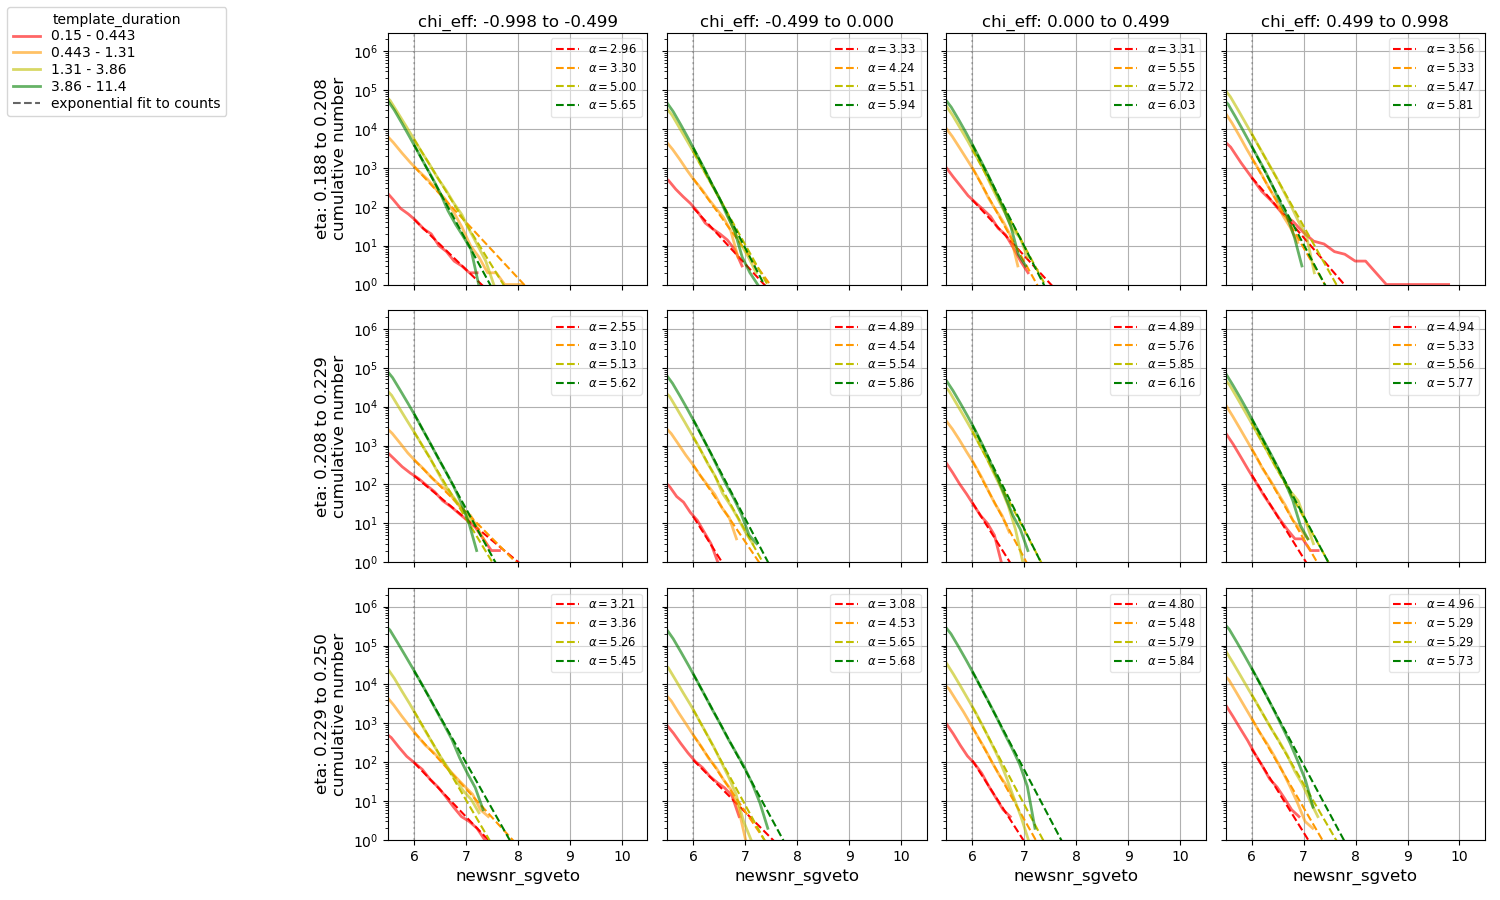
\includegraphics[width=1.0\textwidth]{images/5_pycbclive/H1-template_fits.png}
%     \label{5:fig:template-fits}
  
%     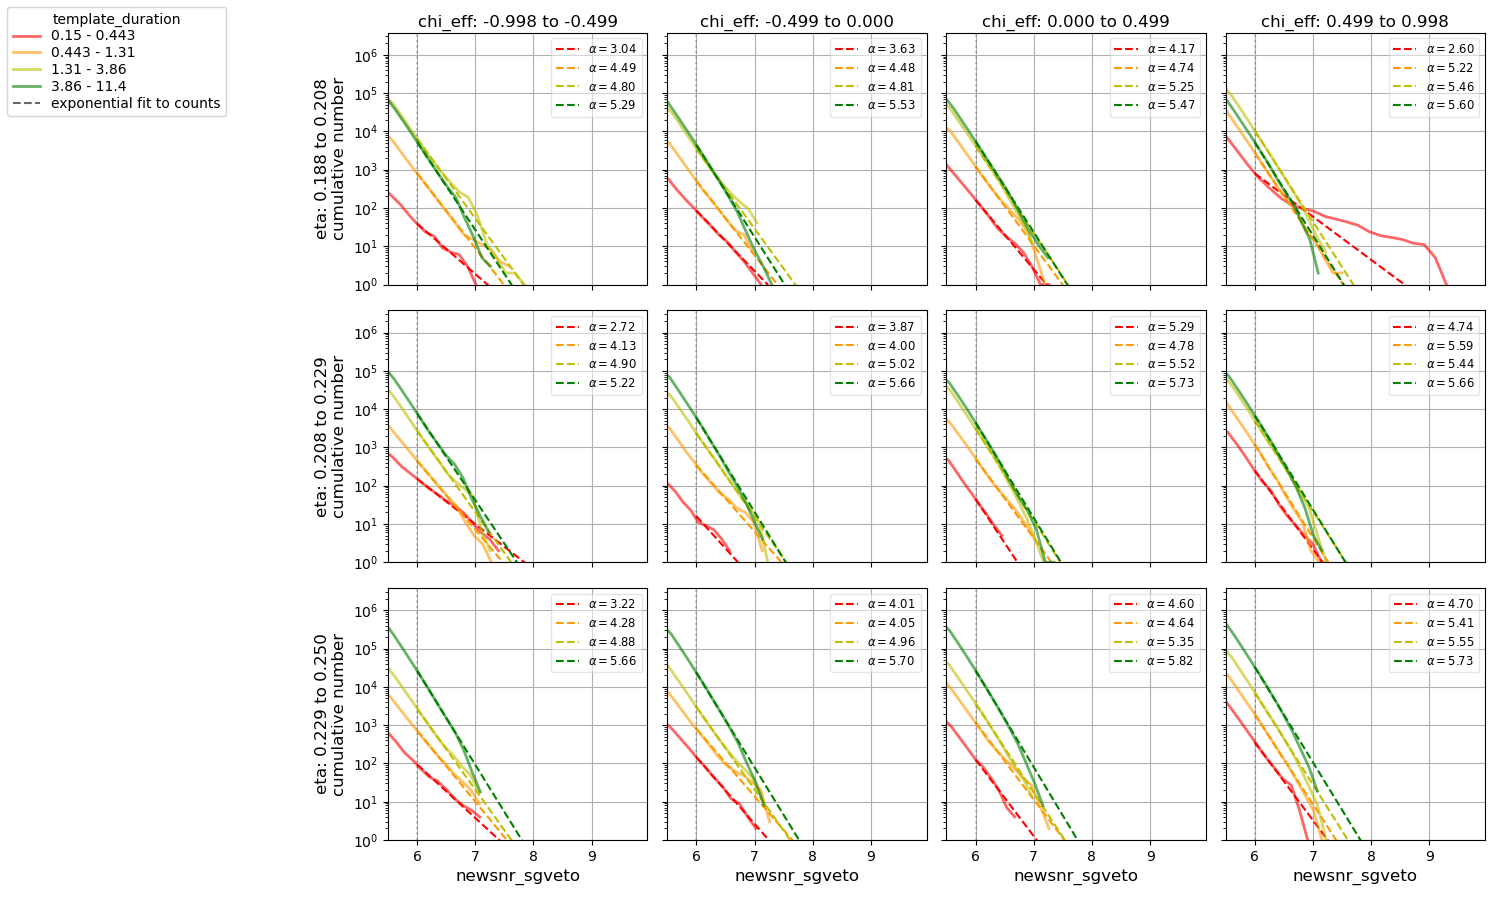
\includegraphics[width=1.0\linewidth]{images/5_pycbclive/L1-template_fits.png}
%     \label{5:fig:L1-fits}

%   \end{minipage}
%   \caption{The noise distributions for 12 discrete bins in the $\chi_{eff}$ and $\eta$ parameter space, with cumulative number on the vertical axis and $\rho_{new}$ on the horizontal axis. Each bin then has four discrete template duration bins plotted on top, alongside the exponential fit factor for each template bin. The top plot represents the triggers from the H1 detector and the bottom plot the L1 detector triggers.}
%   \label{5:fig:template-fits}
% \end{figure}
% %
% An example of template fits generated from a weeks worth of triggers can be seen in figure~\ref{5:fig:template-fits}. These are created from the first week of our injections testing data that was used to calculate increases in the search sensitivity from including the new ranking statistic components. From this figure we can see clearly the difference between `good' and `bad' template fits, a good fit is one with a steep slope (high $\alpha$) and the trigger distribution following closely to the slope line, bad fits have a shallow slop and poor fit to the line. It can be seen in figure~\ref{5:fig:template-fits} that we have binned over three parameters: $\chi_{eff}$, $\eta$, \verb|duration|, and we can see that high $\chi_{eff}$, low $\eta$ and short duration templates have the worst fits, meaning they are more likely to trigger on noise with a high SNR.

\section{\label{5:sec:injection-tests}Measuring Improvements in Search Sensitivity}

% Motivation for investigating the sensitivity increase
% How do we quantify sensitivity
To quantifiably demonstrate that the new additions to the ranking statistic have improved the live search we can investigate the differences in sensitivity when the PSD variation and exponential noise model are included. We quantify the sensitivity of the search by calculating the sensitive volume in which we can observe gravitational wave signals. The sensitive volume is calculated by measuring the detection efficiency of different distance bins that are taken from an injection set and then multiplying by the volume enclosed by the distance bins. The volume of each bin is then summed to find the total sensitive volume of the search~\cite{rw_snr_eq:2012}.

We can search through a period of data which contains an injections set with two instances of the PyCBC Live search, one containing the new ranking statistic additions and one representing the original ranking statistic. The ratio of the new statistic sensitive volume to the original statistic sensitive volume will indicate the change in sensitivity when including the new ranking statistic components.

% What is the injection set
We have chosen to test the ranking statistic changes to PyCBC Live using a smaller template bank than the current PyCBC Live template bank, which contains over $730,000$ templates~\cite{PyCBC_Live:2018}. PyCBC-BBH is a search focussed on binary black hole (BBH) signals performed in the third observing run~\cite{gwtc3:2023, PyCBC_focussed_bbh:2024} and used a template bank with only $15,436$ templates with the drawback that we are only considering BBH signals. This smaller template bank uses fewer computational resources and allows a full week of data to be searched through with PyCBC Live in as little as $1$ day. The injection sets used in the third observing run is shown in table~\ref{5:tab:injection-set}~\cite{gwtc3:2023} with rows for the specific cuts on injections for both the PyCBC-broad (full parameter space search) and PyCBC-BBH search.
% % ORIGINAL TABLE FROM THE PAPER, I'VE REMOVE SOME THINGS
% \begin{table}[]
%     \centering
%     \begin{tabular}{c c cccccc }
%         \multicolumn{2}{c}{ } & Mass & Mass &  Spin & Spin & Redshift & Maximum  \\
%         \multicolumn{2}{c}{ } & distribution & range ($M_{\odot}$) & range & orientations & evolution & redshift  \\
%         \hline
%         \multirow{6}{*}{{Injections}} & \multirow{2}{*}{BBH} &  $\left.p(m_{1}) \propto m_{1}{}^{-2.35}\right.$ \rule{0pt}{1.05\normalbaselineskip} & $2 < m_{1} < 100$ & \multirow{2}{*}{$\left|\chi_{1,2}\right| < 0.998$} & \multirow{2}{*}{Isotropic} & $ \multirow{2}{*}{$\kappa = 1$}$ & \multirow{2}{*}{$1.9$}  \\
%          & & $p(m_{2}|m_{1}) \propto m_{2}$ & $2 < m_{2} < 100$ & & & & \\[0.05\normalbaselineskip]
%          & \multirow{2}{*}{NSBH} & $\left.p(m_{1}) \propto m_{1}^{-2.35}\right.$ & $2.5 < m_{1} < 60$ & $\left|\chi_1\right| < 0.998$ & \multirow{2}{*}{Isotropic} & $ \multirow{2}{*}{$\kappa = 0$}$ &  \multirow{2}{*}{$0.25$} \\
%          & & Uniform & $1 < m_{2} < 2.5$ & $\left|\chi_2\right| < 0.4$ & & &  \\[0.05\normalbaselineskip]
%          & \multirow{2}{*}{BNS} & \multirow{2}{*}{Uniform} & $1 < m_{1} < 2.5$ & \multirow{2}{*}{$\left|\chi_{1,2}\right| < 0.4$} & \multirow{2}{*}{Isotropic} & $ \multirow{2}{*}{$\kappa = 0$}$ & \multirow{2}{*}{$0.15$}  \\
%          & & & $1 < m_{2} < 2.5$ & & & & \\%[0.25\normalbaselineskip]
%         \hline
%         \multirow{3}{*}{PyCBC-broad $p_{astro}$} & BBH & & $\mathcal{M} > 4.353 $ & & & & \\[0.05\normalbaselineskip]
%         & NSBH & & \hspace{-1.25cm} $ 2.176 < \mathcal{M} < 4.353 $ & & & & \\[0.05\normalbaselineskip]
%         & BNS & & $ \mathcal{M} < 2.176 $ & & & & \\%[0.25\normalbaselineskip]
%         \hline
%         {PyCBC-BBH $p_{astro}$} & {BBH} & & $\mathcal{M} > 4.353 $ & & & \\
%     \end{tabular}
% \end{table}
% %
%
\begin{table}[ht]
    \centering
    \begin{tabular}{c c ccc }
        \multicolumn{2}{c}{ } & Mass & Mass &  Spin \\
        \multicolumn{2}{c}{ } & distribution & range ($M_{\odot}$) & range  \\
        \hline
        \multirow{6}{*}{{Injections}} & \multirow{2}{*}{BBH} &  $\left.p(m_{1}) \propto m_{1}{}^{-2.35}\right.$ \rule{0pt}{1.05\normalbaselineskip} & $2 < m_{1} < 100$ & \multirow{2}{*}{$\left|\chi_{1,2}\right| < 0.998$} \\
         & & $p(m_{2}|m_{1}) \propto m_{2}$ & $2 < m_{2} < 100$ & \\[0.05\normalbaselineskip]
         & \multirow{2}{*}{NSBH} & $\left.p(m_{1}) \propto m_{1}^{-2.35}\right.$ & $2.5 < m_{1} < 60$ & $\left|\chi_1\right| < 0.998$ \\
         & & Uniform & $1 < m_{2} < 2.5$ & $\left|\chi_2\right| < 0.4$  \\[0.05\normalbaselineskip]
         & \multirow{2}{*}{BNS} & \multirow{2}{*}{Uniform} & $1 < m_{1} < 2.5$ & \multirow{2}{*}{$\left|\chi_{1,2}\right| < 0.4$} \\
         & & & $1 < m_{2} < 2.5$ & \\%[0.25\normalbaselineskip]
        \hline
        \multirow{3}{*}{PyCBC-broad} & BBH & & $\mathcal{M} > 4.353 $ & \\[0.05\normalbaselineskip]
        & NSBH & & \hspace{-1.25cm} $ 2.176 < \mathcal{M} < 4.353 $ & \\[0.05\normalbaselineskip]
        & BNS & & $ \mathcal{M} < 2.176 $ & \\%[0.25\normalbaselineskip]
        \hline
        {PyCBC-BBH} & {BBH} & & $\mathcal{M} > 4.353 $ \\
    \end{tabular}
    \caption{Recreated from~\cite{gwtc3:2023}. The intrinsic parameter distributions used to generate the injection set used for computing the sensitive volume change when including the PSD variation statistic and exponential noise model. Here PyCBC-broad is the PyCBC offline search across the full template bank and parameter space, including templates representing binary black hole, neutron star black hole and binary neutron star signals. This is comparable to the template bank used by the PyCBC Live full-bandwidth search. PyCBC-BBH considers only templates with chirp mass, $\mathcal{M}$, greater than $4.353 M_{\odot}$ which includes only binary black hole signals. This is the same template bank that is used for the analysis in this chapter.}
    \label{5:tab:injection-set}
\end{table}
%
%
% DESCRIBE WHY THE TEST IS STILL REPRESENTATIVE JUST USING THE BBH INJECTIONS

% How did we test the search changes
As previously mentioned, the template fits are measured from the triggers found in the previous week to the week currently being searched through. Therefore to perform our injection set test we need to do an initial search with PyCBC Live using the original ranking statistic to generate a weeks worth of triggers and create template fit statistics. The second week of data is then created containing a large number of injected gravitational wave signals that is searched through with PyCBC Live using both the original ranking statistic and the new ranking statistic. The two weeks of O3b gravitational wave data used lasted from 06 January 2020 23:59:42 to 20 January 2020 23:59:42 and, according to the gravitational wave catalogue for the third observing run~\cite{gwtc3:2023}, there were no real gravitational wave signals present. After both searches have completed analysing the second week of data we can estimate the sensitivity improvement. We can choose a threshold false-alarm rate (FAR) and count the number of injections in both searches that have been found with a FAR lower than that number, if the counted number of injections is higher when including the new ranking statistic additions we have seen an increase in the sensitivity of the search. We can do this for a range of FAR values from $10^{4} - 10^{-4}$ to build up a picture of the sensitivity ratio curve.

\section{\label{5:sec:sensitivity-improvements}Improvements in Sensitivity}

By adding the PSD variation and the exponential noise model to the ranking statistic we expect to find gravitational wave injections with a greater significance than before. This significance is determined by the FAR of the injection, which has a direct mapping to the ranking statistic value, an event found with a FAR of $1$ per year would indicate that an event with the exact same parameters is expected to be seen in the data caused by non-astrophysical noise-not a real event-once per year of analysis time. We commonly use the inverse false-alarm rate (IFAR) with units of $years$ where a large IFAR indicates a more confident detection. An IFAR threshold is chosen to separate events which are real from those that are false alarms, a balance must be made to avoid contaminating the detection catalogue with a large number of potential false alarms while not missing any real events. In this analysis we are considering only two detectors, allowing potentially more false-alarms from coincident noise when compared to a three detector configuration and therefore we have chosen a more conservative IFAR threshold of $1$ year to assess sensitivity improvements. The current threshold for LIGO/Virgo alert generation is $1$ per $2$ months~\cite{PyCBC_Live:2018} so low-latency gravitational wave searches will identify more gravitational wave events but these detections have additional post detection checks from data quality checks from detector characterisation~\cite{O2O3_DetChar:2021} and parameter estimation~\cite{gwtc3:2023} which can also rule out false-alarms and to prevent catalogue contamination.

% This is a low latency search so a threshold is hard to determine concretely.

% How do we compare sensitivity of the two searches using the significance of the injections
To measure the sensitivity improvement of the new ranking statistic we count the number of injections found by both searches over a range of IFAR values from $10^{-4} - 10^{4}$ and take the ratio of the counts. The injection set is pre-weighted to ensure each injection represents an equal volume, therefore instead distance binning, as described in section~\ref{5:sec:injection-tests}, we can simply count the number of injections seen by each search.
% Sensitivity Increase Plot
%
\begin{figure}
  \centering
  \begin{minipage}[t]{1.0\linewidth}
  
    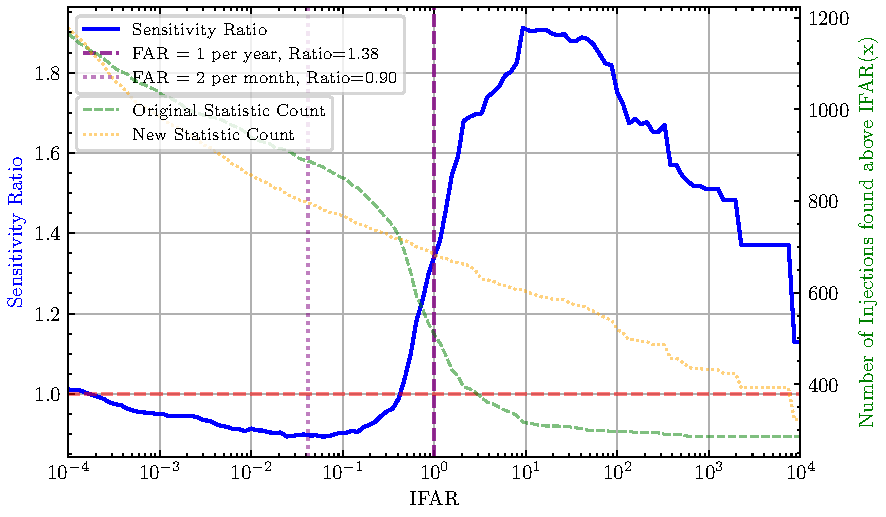
\includegraphics[width=1.0\textwidth]{images/5_pycbclive/fits-psd/fits_psd_vt_ratio_with_counts.pdf}
    \caption{The sensitive volume ratio between a PyCBC Live search whose ranking statistic contains PSD variation and an exponential noise model and a PyCBC Live search using the original ranking statistic used by PyCBC Live during the third observing run as a function of inverse false alarm rate (IFAR). The blue curve represents the sensitivity ratio computed by comparing the number of injections detected with an IFAR exceeding the corresponding x-axis value. An increase in sensitivity is indicated by values greater than 1, the horizontal red-dashed line. Two vertical dashed lines at fixed false-alarm rates (FAR) highlight specific thresholds: FAR = 1 per year (dark purple, dashed) with a sensitivity ratio of 1.38, and FAR = 2 per month (light purple, dotted) with a sensitivity ratio of 0.90. The green and orange curves represent the cumulative number of injections detected in the old and new searches, respectively, as a function of IFAR.}
    \label{5:fig:fits-psdvar-sensitivity}

  \end{minipage}
\end{figure}
%
% Comments about the weird shape of the plot
Figure~\ref{5:fig:fits-psdvar-sensitivity} shows the sensitivity ratio plot comparing the new statistic search to the original statistic search. We see $35\%$ more injections with an IFAR greater than our threshold of $1$ year which is a very large increase in sensitivity however at a FAR of $2$ per month we see a sensitivity decrease of $10\%$. To understand the shape of the sensitivity curve we can look at the new additions to the ranking statistic and understand further how they are changing the significance of individual injections.

\section{\label{5:sec:injection-investigations}Changes in Injection Significance}

% How do we map from Ranking Stat to FAR??

% How do IFAR and Significance relate
\begin{figure}
      \centering
    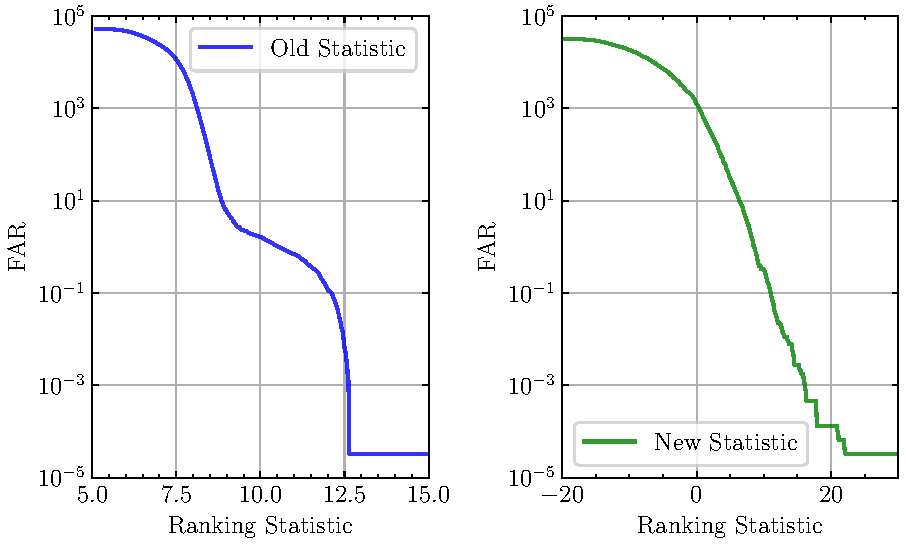
\includegraphics[width=1.0\textwidth]{images/5_pycbclive/fits-psd/fits_psd_far_vs_stat.pdf}
    \caption{The mapping between false-alarm rate (FAR) and ranking statistic for the original PyCBC Live ranking statistic used in the third observing run (left, blue) and the new PyCBC Live ranking statistic including PSD variation and an exponential noise model (right, green). Ranking statistic values cannot be compared between ranking statistics but injection FARs can be. Higher ranking statistic values indicate better, lower FARs. The original ranking statistic has a narrower range of allowed ranking statistic values ($5 - 12.5$) along with a distinct curvature whereas the new statistic ranking statistic can take a broader range of ranking statistic values ($-20-22$) and has a relatively smooth drop off with increasing ranking statistic values.}
    \label{5:fig:fits-psdvar-far-stat}
\end{figure}
%
The ranking statistic assigned to each event can be mapped directly to FAR, shown in figure~\ref{5:fig:fits-psdvar-far-stat}. Changing the ranking statistic calculation will lead to incomparable values between searches but the individual injection IFAR values can be compared. The PyCBC Live search will matched filter the template bank and the data and where the resulting $\rho$ and $\hat{\rho}$ is above pre-defined thresholds (both $4.5$ in the third observing run) the trigger is kept. The coincidence ranking statistic value is calculated and then a ranking statistic value is assigned to the event. The initial $\rho$ values are the same between the two searches because these depend only on template and data but $\hat{\rho}$ depends on the single detector ranking statistic which has the addition of PSD variation in our new statistic, therefore it is possible for the PSD variation to prevent the saving of a trigger due to a trigger's $\hat{\rho}$ being re-weighted below the threshold.

% How does the new statistic change the injections found
We can plot the IFAR value of each injection that has been found in both searches, seen in 
figure~\ref{5:fig:ifar-ifar-fits-psdvar-shaded}.
%
\begin{figure}
      \centering
    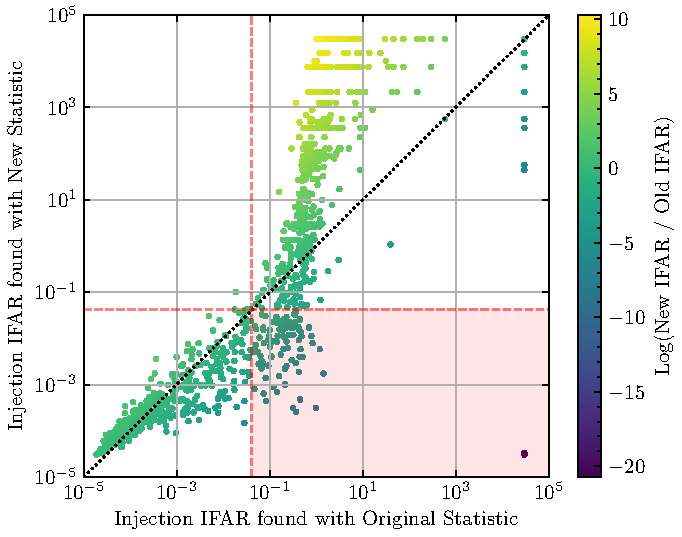
\includegraphics[width=1.0\textwidth]{images/5_pycbclive/fits-psd/fits_psd_ifar_vs_ifar_shaded_region.pdf}
    \caption{The inverse false alarm rate (IFAR) values recorded for each injection that was seen by both the PyCBC Live search that includes the PSD variation and exponential noise model in the ranking statistic and the PyCBC Live search using the same ranking statistic as used in the third observing run. Each point represents an injection from the injection set, with the x-axis showing the IFAR recorded using the original ranking statistic and the y-axis showing the IFAR recorded using the new ranking statistic. The color bar indicates the logarithmic difference in IFAR between the two searches, with positive values (yellow) indicating better performance of the new statistic and negative values (purple) indicating a worse performance with the new statistic. The dashed line at y=x represents equal IFAR values for both searches. The vertical and horizontal red dashed lines denote a false-alarm rate threshold of $2$ per month. The highlighted region in the bottom right of the plot indicates excess injections that have been seen by the original ranking statistic above the $2$ per month threshold and by the new ranking statistic below the $2$ per month threshold.}
    \label{5:fig:ifar-ifar-fits-psdvar-shaded}
\end{figure}
%
Within figure~\ref{5:fig:ifar-ifar-fits-psdvar-shaded} we have plotted a line on the diagonal $y=x$, injections above this line ($y > x$) have been found with a larger IFAR with the new ranking statistic and injections below ($y < x$) have been found with a lower IFAR with the new statistic. Figure~\ref{5:fig:fits-psdvar-sensitivity} highlighted the decrease in sensitivity at a FAR of $2$ per month, this decrease is due to an excess number of injections in the red-shaded box in the bottom-right of figure~\ref{5:fig:ifar-ifar-fits-psdvar-shaded}, this region represents injections which have been found by the original ranking statistic below a FAR of $2$ per month but with a FAR above $2$ per month when found by the new ranking statistic. Understanding why these injections have been down-ranked by the new statistic is crucial.

\subsection{\label{5:sec:ignoring-psdvar}Effects of PSD Variation on Sensitivity}

The injections shown in figure~\ref{5:fig:ifar-ifar-fits-psdvar-shaded} that lie below the $y = x$ diagonal line have been found with a lower significance when including the PSD variation and the exponential noise model in the ranking statistic. We can separate the new additions and investigate the individual contributions to the changes in sensitivity.

The PSD variation statistic measures the non-stationary noise in the data and applies a weighting to the trigger $\rho$ value calculated by the matched filter of template and data, prior to the calculation of $\hat{\rho}$. To understand the effect of the PSD variation statistic on the injection significance we can compare the IFAR of injections found by the new statistic which includes both the PSD variation statistic and the exponential noise model and the IFAR of the same injections but with only the addition of the exponential noise model. This comparison is shown in figure~\ref{5:fig:ifar-ifar-fits-vs-fits-psdvar}
%
\begin{figure}
       \centering
    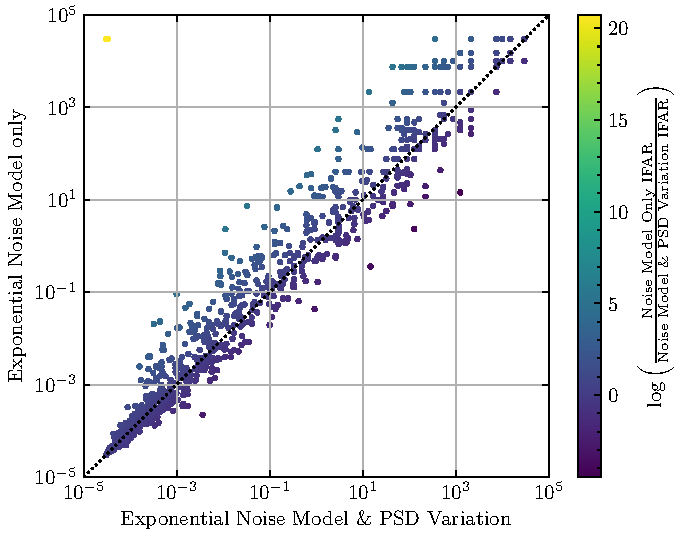
\includegraphics[width=1\textwidth]{images/5_pycbclive/fits-only/fits_only_fits_psd_var_ifar_vs_ifar.pdf}
    \caption{The inverse false alarm rate (IFAR) values recorded for injections that were seen by both the PyCBC Live search that includes new additions of the PSD variation statistic and exponential noise model in the ranking statistic and the PyCBC Live search which has new additions of only the exponential noise model. Each point represents an injection from the injection set, with the x-axis showing the IFAR recorded by the PyCBC Live search including the exponential noise model and PSD variation ranking statistic and the y-axis showing the IFAR recorded by the PyCBC Live search which has added only the exponential noise model. The color bar indicates the logarithmic difference in IFAR between the two searches, with positive values (yellow) indicating better performance when \textbf{not} including PSD variation and negative values (purple) indicating a better performance with the PSD variation statistic. The dashed line at y=x represents equal IFAR values for both searches.}
    \label{5:fig:ifar-ifar-fits-vs-fits-psdvar}
\end{figure}
%
In this comparison, $550$ injections were found with a higher significance when \textbf{not} including PSD variation, $399$ were found with a higher IFAR when including PSD variation and $326$ were found with the same IFAR. We can also observe a greater dispersion of injections found above the diagonal line when compared to those found below it, meaning injections found above the diagonal line are found with a greater significance difference than those found below the line. Alongside this general trend we can see a few injections in the top-left of the plot which have had a very large increase in significance when we do not include PSD variation in the statistic, these injections correspond to the heavily down-ranked injections in the bottom-right of figure~\ref{5:fig:ifar-ifar-fits-psdvar-shaded}.

% Talk about sensitivity difference
We can compare the sensitivity change when including the PSD variation statistic by plotting the sensitivity curve in figure~\ref{5:fig:vt-ratio-f-fo}.
%
\begin{figure}
       \centering
    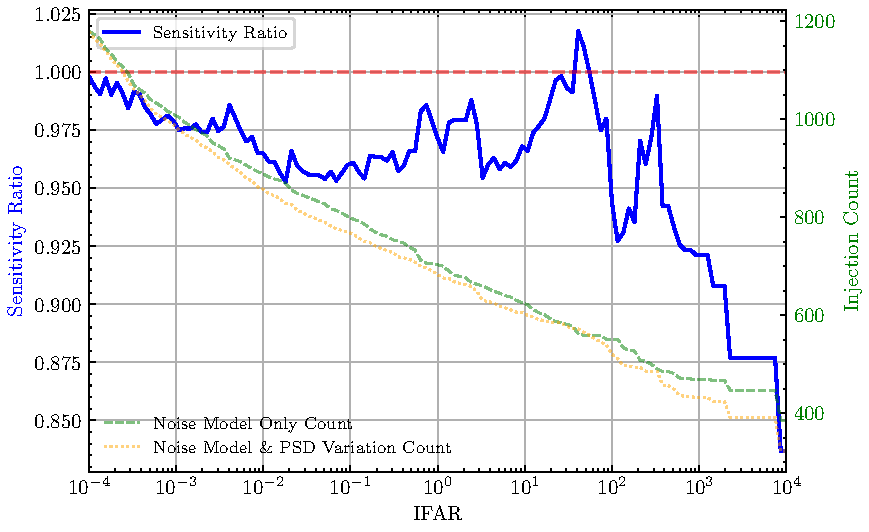
\includegraphics[width=1.0\textwidth]{images/5_pycbclive/fits-only/fits_only_fits_psd_vt_ratio.pdf}
    \caption{A comparison of sensitive volume ratio between two PyCBC Live searches: one which includes the addition of the PSD variation statistic and an exponential noise model in the ranking statistic and one which includes only the addition of the exponential noise model. The blue curve represents the sensitivity ratio computed by comparing the number of injections detected with an inverse false-alarm rate (IFAR) exceeding the corresponding x-axis value. An increase in sensitivity is indicated by values greater than 1, the horizontal red-dashed line. The green dashed curve represents the cumulative number of injections detected as a function of IFAR by the PyCBC Live search with added PSD variation and the exponential noise model. The orange dashed curve represents the cumulative number of injections detected as a function of IFAR by the PyCBC Live search with only the exponential noise model added.}
    \label{5:fig:vt-ratio-f-fo}
\end{figure}
%
From which is it clear to see there is a decrease in sensitivity when including the PSD variation statistic in the new ranking statistic.

We have previously described how the PyCBC Live search re-calculates the PSD every analysis segment and replaces the currently used PSD when the BNS distance of the new PSD differs from the current PSD's by more than $1\%$. This reduces the need to include the PSD variation statistic to tackle non-stationary noise in the data. In light of the sensitivity decrease when including PSD variation we make the choice to not use PSD variation in the ranking statistic going forward.

% Noise model only sensitivity
When adding only the exponential noise model to the ranking statistic we can re-analyse the sensitivity improvements to produce figure~\ref{5:fig:vt-ratio-fits-only}.
%
\begin{figure}
       \centering
    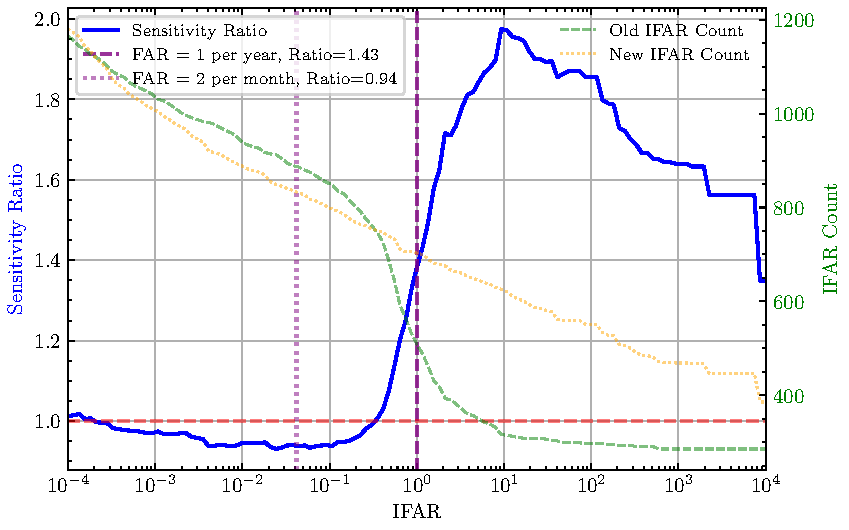
\includegraphics[width=1.0\textwidth]{images/5_pycbclive/fits-only/fits_only_vt_ratio_with_counts.pdf}
    \caption{A comparison of sensitive volume ratio between a PyCBC Live search whose ranking statistic contains an exponential noise model and a PyCBC Live search using the original ranking statistic used by PyCBC Live during the third observing run as a function of inverse false alarm rate (IFAR). The blue curve represents the sensitivity ratio computed by comparing the number of injections detected with an IFAR exceeding the corresponding x-axis value. An increase in sensitivity is indicated by values greater than 1, the horizontal red-dashed line. Two vertical dashed lines at fixed false-alarm rates (FAR) highlight specific thresholds: FAR = 1 per year (dark purple, dashed) with a sensitivity ratio of 1.43, and FAR = 2 per month (light purple, dotted) with a sensitivity ratio of 0.94. The green and orange curves represent the cumulative number of injections detected in the old and new searches, respectively, as a function of IFAR.}
    \label{5:fig:vt-ratio-fits-only}
\end{figure}
%
Which shows a greater increase across the IFAR range, with sensitivity increase at a FAR of $1$ per year of $43\%$ and a decrease of $6\%$ at a FAR of $2$ per month.

% Noise model only IFAR vs IFAR with regions
We can plot the IFAR vs IFAR plot for the search including only the exponential noise model in the ranking statistic compared to the original search, seen in figure~\ref{5:fig:ifar-ifar-fits-only-regions}, and when we compared to figure~\ref{5:fig:ifar-ifar-fits-psdvar-shaded} we can see that the distribution of injections at low IFARs has decreased in dispersion around the diagonal line.
% 
\begin{figure}
       \centering
    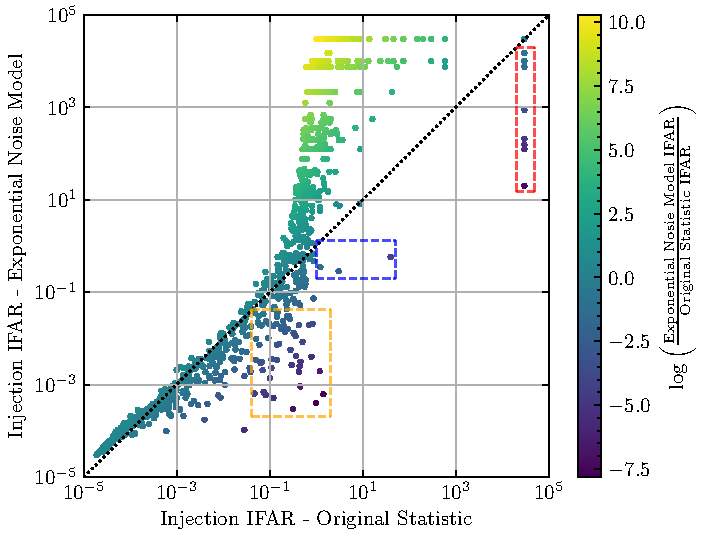
\includegraphics[width=1.0\textwidth]{images/5_pycbclive/fits-only/fits_only_ifar_vs_ifar_regions.pdf}
    \caption{The inverse false alarm rate (IFAR) values recorded for each injection that was seen by both the PyCBC Live search that includes the exponential noise model in the ranking statistic and the PyCBC Live search using the same ranking statistic used in the third observing run. Each point represents an injection from the injection set, with the x-axis showing the IFAR recorded using the original ranking statistic and the y-axis showing the IFAR recorded using the exponential noise model ranking statistic. The color bar indicates the logarithmic difference in IFAR between the two searches, with positive values (yellow) indicating better performance when including the exponential noise model in the statistic and negative values (purple) indicating a better performance with the original statistic. The dashed line at y=x represents equal IFAR values for both searches. Three regions containing injections that have been down-ranked and will be investigated have been highlighted in dashed boxes.}
    \label{5:fig:ifar-ifar-fits-only-regions}
\end{figure}
%
We have highlighted three regions of interest which contains injections that have decreased in significance that we will investigate further and understand the cause of their down-ranking.

\subsection{\label{5:sec:poor-temp-fits}Templates which Trigger Frequently with Large SNRs}

% Log(noise rate) equation
% Combined log(noise rate) equation
% Low Alpha + High Rate == High Combined Log(noise rate)
% Plot Alpha vs Rate, colour Log(noise rate)
% Plot Alpha vs SNR, colour Log(noise rate)

% Motivation here is the separation of PSD Variation and Template Fits to see how they change the sensitivity of each injection or how the sensitivity change manifests

% What identifies a template as having a high noise rate
The new exponential noise model in the ranking statistic allows us to model individual template noise distributions depending using that template's historical triggers. This allows us to down-rank templates which frequently trigger on non-Gaussian noise with a high $\hat{\rho}$. As describe in equation~\ref{5:eqn:comb-noise-rate}, the exponential noise model is characterised by an exponential fit to the slope of the trigger distribution and is quantified by the exponential fit factor, $\alpha$, and the count of triggers above $\hat{\rho}_{thresh}$, $\mu$. Therefore, using these two parameters we must be able to differentiate between templates which trigger frequently on noise with large $\hat{\rho}$ and those that rarely trigger on noise. All templates in the bank will trigger on both Gaussian noise and glitches in our data, and after applying all signal consistency tests these triggers might still might have $\hat{\rho} > 8.0$. 

Figure~\ref{5:fig:template-fits} shows an example of the exponential fitting to a group of template's noise distributions to obtain the exponential fit factors. This group of templates have effective spin, $\chi_{eff} = -0.333 - 0.333$, symmetric mass ratio $\eta = 0.208 - 0.229$ and the different template duration bins and corresponding exponential fitting factors have been plotted over the top.
%
\begin{figure}
    \centering
    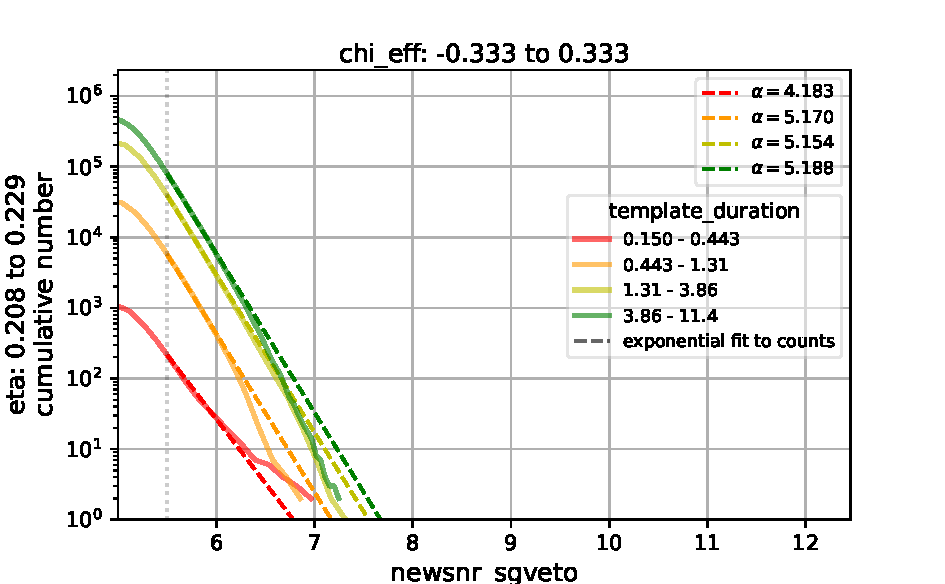
\includegraphics[width=1.0\textwidth]{images/5_pycbclive/others/fit_plot.pdf}
    \caption{The noise distribution and template fits for a bin which contains triggers from templates which have symmetric mass ratio, $\eta$, between $0.208 - 0.229$ and effective spin, $\chi_{eff}$, between $-0.333 - 0.333$. The template triggers are further split into 4 bins depending on the duration of the template responsible for the trigger (in seconds). The solid coloured lines represent the cumulative counts of triggers that have been found in a template duration bin with $\rho$ that has been re-weighted by the traditional $\chi^{2}$~\cite{Allen_Chi:2005} and the sine-gaussian $\chi^{2}$~\cite{PyCBC_sg:2018} to obtain new signal-to-noise ratio, $\hat{\rho}$. The dashed coloured lines represent the exponential fit that has been made to the cumulative counts for each template duration bin where the exponential fit factor value, $\alpha$, is displayed in the top right most legend.}
    \label{5:fig:template-fits}
\end{figure}
%
This figure shows the difference in exponential fit slopes for the varying template bins and it can be seen that the bins which trigger more frequently with a higher new SNR have shallower slopes (lower $\alpha$) compared to the steeper slopes (higher $\alpha$) in other bins. Equation~\ref{5:eqn:single-log-noise-rate} shows that higher $\alpha$ values correspond to lower noise rates and lower $\alpha$ and higher $\mu$ values produce higher noise rates.

Templates which trigger more frequently and with a large $\hat{\rho}$ on noise will be down ranked by the ranking statistic but real gravitational wave signals that match this template will also be down ranked if they have low single detector $\hat{\rho}$. We can plot equation~\ref{5:eqn:single-log-noise-rate}, which calculates the single detector noise rate, in figure~\ref{5:fig:log-noise-static-snr} to show the dependence on $\alpha$ and $\mu$. In our search $\alpha$ can take values $1.5 - 6.0$ and $\mu$ from $5 - 45$ and we have used a static $\hat{\rho}$ of $10.0$ in the equation. It can be seen that a higher $\alpha$ value has a greater effect on the noise rate and the contribution from $\mu$ has a maximum value of $3.8$, $ + \log\mu$ in equation~\ref{5:eqn:single-log-noise-rate}.
%
\begin{figure}
    \centering
    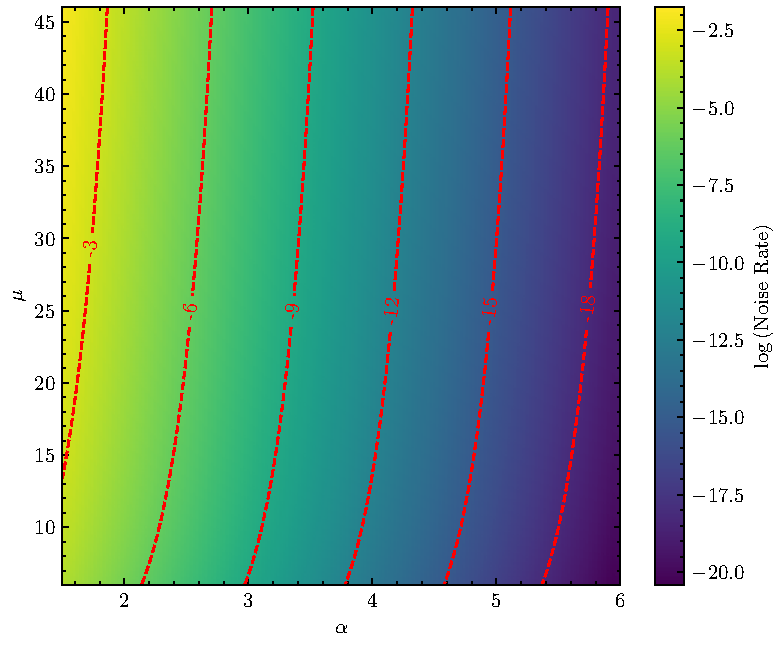
\includegraphics[width=1\textwidth]{images/5_pycbclive/high-noise-rate/lognoise_alpha_rate.pdf}
    \caption{The single detector ($\log$) noise rate for varying combinations of exponential fit factor, $\alpha$, and trigger rates above a single detector statistic value ($\hat{\rho}_{thresh} = 6.0$), $\mu$. Constant contours of single detector noise rate are shown as dashed red lines, with the single detector noise rate value labelled within the contour line. This figure has been made using equation~\ref{5:eqn:single-log-noise-rate} where $\hat{\rho} = 10.0$.}
    \label{5:fig:log-noise-static-snr}
\end{figure}
%
Figure~\ref{5:fig:log-noise-static-rate} shows the noise rate's dependence on $\alpha$ and $\hat{\rho}$ while $\mu$ has been set to the benchmark noise rate of $-14.6$, which is the representative noise rate measured empirically during the second observing run. 
%
\begin{figure}
    \centering
    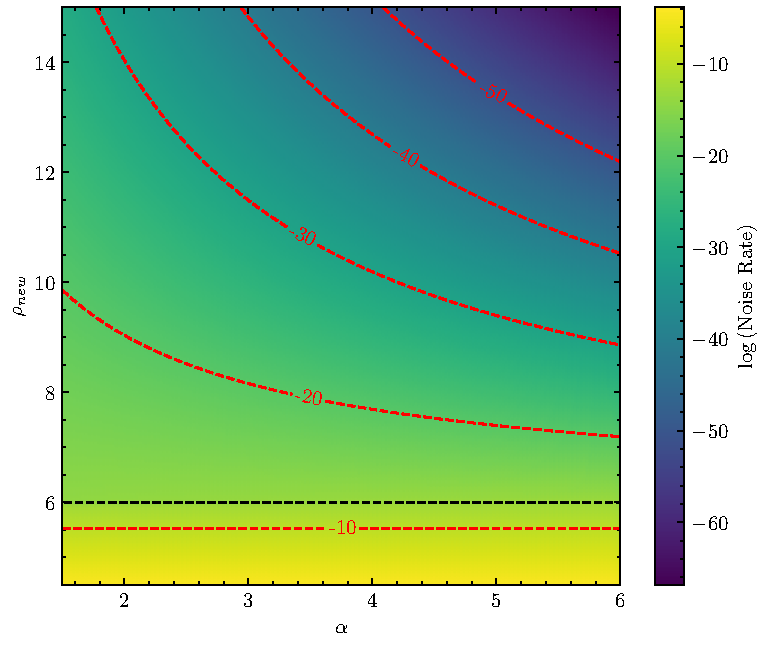
\includegraphics[width=1\textwidth]{images/5_pycbclive/high-noise-rate/lognoise_alpha_snr.pdf}
    \caption{The single detector ($\log$) noise rate for varying combinations of exponential fit factor, $\alpha$, and single detector statistic value, $\hat{\rho}$. Constant contours of single detector noise rate are shown as dashed red lines, with the single detector noise rate value labelled within the contour line. This figure has been made using equation~\ref{5:eqn:single-log-noise-rate} where $\mu$ has been set equal to the benchmark noise rate $-14.6$.}
    \label{5:fig:log-noise-static-rate}
\end{figure}
%
A black dashed line has been plotted at $\hat{\rho} = 6.0$ due to triggers below this $\hat{\rho}$ threshold all being assigned $\alpha = 6.0$, therefore the noise rate below this threshold is constant for all $\alpha$ values on the plot. We can clearly see a strong correlation between $\hat{\rho}$ and noise rate with a heavy dependency on $\alpha$, to the point where high $\hat{\rho}$ triggers with low $\alpha$--while still significant--have higher noise rates than triggers with high $\alpha$.

% Plot IFAR vs IFAR, colour H1 alpha
% Plot IFAR vs IFAR, colour H1 rate
% Plot IFAR vs IFAR, colour H1 noise rate

We can plot the IFAR vs IFAR distribution for the injection set for a single detector's $\alpha$, $\mu$ and log noise rate to see if there is any clear dependence on the template fit parameters, seen in figures~\ref{5:fig:ifar-ifar-subplots}.
%
\begin{figure}
    \centering
    \includegraphics[width=\textwidth]{images/5_pycbclive/fits-only/fits_only_ifar_vs_ifar_subplots.pdf}
    \caption{The inverse false alarm rate (IFAR) values recorded for each injection that was seen by both the PyCBC Live search that includes the exponential noise model in the ranking statistic and the PyCBC Live search using the same ranking statistic used in the third observing run. Each point represents an injection from the injection set, with the x-axis showing the IFAR recorded using the original ranking statistic and the y-axis showing the IFAR recorded using the exponential noise model ranking statistic. The top left plot is coloured by the LIGO-Hanford trigger template's exponential fit factor, $\alpha$. The top right plot is coloured by the LIGO-Hanford trigger template's count of triggers found above $\hat{\rho}_{threshold} = 6.0$, $\mu$. The bottom left plot is coloured by the LIGO-Hanford single detector ($\log$) noise rate, calculated using equation~\ref{5:eqn:single-log-noise-rate}. The bottom right plot is coloured by the combined ($\log$) noise rate, equation~\ref{5:eqn:comb-log-noise-rate}.}
    \label{5:fig:ifar-ifar-subplots}
\end{figure}
%
It is not clear from these figures that $\alpha$ (top-left) and $\mu$ (top-right) are having a large effect on the log noise shown in the bottom-left figure. There is a curve of high $\alpha$ points above the $y=x$ line in the top-left figure but no clear distinction between higher and lower $\alpha$ values corresponding to higher and lower IFAR values. As mentioned before and reinforced by the top-right plot, $\mu$ has a small effect on the noise rate and low $\mu$ values are more common than high ones.

Figure~\ref{5:fig:ifar-ifar-subplots} shows the combined detector noise rates (equation~\ref{5:eqn:comb-log-noise-rate}), where we can see a clearer distinction between high and low noise rates and how this is affecting the IFAR values. However, looking at this plot we can see that combined noise rate does not completely explain the improved significance for a number of injections, we can see clearly there are some low noise rate injections below the $y=x$ line which should have caused an increase in the significance but we have seen a decrease. Therefore we must investigate other changes to the ranking statistic.

\subsection{\label{5:sec:comparing-statistic-construction}Ranking Statistic Construction}

% Motivation
The original ranking statistic and our new ranking statistic both take contributions from the signal event rate density, $p^{S}(\Vec{\theta})$, and the noise event rate density, $p^{N}(\Vec{\theta})$. The construction of these ranking statistics has been detailed in sections~\ref{5:sec:old-stat-construction} and~\ref{5:subsec:template-fits} where it can be seen they include the contributions from $p^{S}(\Vec{\theta})$ differently. For comparison, the original statistic is constructed as,
%
\begin{equation}
    R = \sqrt{\hat{\rho}^{2}_{H} + \hat{\rho}^{2}_{L} + 2\log\left(p^{S}(\Vec{\theta})\right)}
    \label{5:eqn:original-statistic-repeat}
\end{equation}
%
and the statistic including the exponential noise model is,
%
\begin{equation}
    R = \log p^{S}(\Vec{\theta}) - \log\left(A_{N}\right) + \sum_{d} \log\left(r_{d}(\hat{\rho})\right),
    \label{5:eqn:new-statistic}
\end{equation}
%
where $p^{N}(\Vec{\theta})$ has been substituted with the combined noise rate defined in equation~\ref{5:eqn:comb-log-noise-rate}.

The general detection statistic (equation~\ref{5:eqn:general-detection-statistic}) was constructed so that in stationary, Gaussian noise the ranking statistic recovers the quadrature sum ranking statistic. When including the exponential noise model we are explicitly modelling the detector noise and therefore have chosen to use the optimal detection statistic (equation~\ref{5:eqn:optimal-detection-statistic}) which is simply the ratio of signal and noise event rate densities.

Equations~\ref{5:eqn:original-statistic-repeat} and~\ref{5:eqn:new-statistic} show that the original statistic quadratically adds signal rate and noise rate whereas the new noise distribution model ranking statistic will add signal and noise rates linearlly, changing the ratio of contributions from signal rate and noise rate in the ranking statistic calculation.

One particular way the different noise rate models manifests is in the ratio of the two detector $\hat{\rho}$ values. Modelling the noise distribution falloff as Gaussian causes the ranking statistic to attempt to maximise the squared sum of the $\hat{\rho}$ values found by each detector with only the signal-consistency tests to re-weight $\rho$. Our new model adds additional weights in the form of the template fits so that if a different trigger is seen with slightly lower $\hat{\rho}$ in both detectors but the template has a lower noise rate (by having higher $\alpha$ and lower $\mu$), then it will be preferred by the noise rate model. Figure~\ref{5:fig:ifar-ifar-snr-ratio} shows the injections coloured by the SNR ratio in the new statistic search.
%
\begin{figure}
  \centering
  \begin{minipage}[t]{1.0\linewidth}
    \includegraphics[width=1\textwidth]{images/5_pycbclive/regions/fits_only_ifar_vs_ifar_regions_snr_ratio.pdf}
  \end{minipage}
  \caption{The inverse false alarm rate (IFAR) values recorded for each injection that was seen by both the PyCBC Live search that includes the exponential noise model in the ranking statistic and the PyCBC Live search using the same ranking statistic used in the third observing run. Each point represents an injection from the injection set, with the x-axis showing the IFAR recorded using the original ranking statistic and the y-axis showing the IFAR recorded using the exponential noise model ranking statistic. The injections are coloured by the SNR ratio of the two detector $\hat{\rho}$ values, set so that the SNR ratio is always greater than $1$. Three regions containing injections that will be investigated have been highlighted in dashed boxes.}
  \label{5:fig:ifar-ifar-snr-ratio}
\end{figure}
%
It can be seen that there are a number of points in regions of interest that have been down-ranked by the new search specifically because they have a high SNR ratio in the old statistic.


\subsection{\label{5:sec:diff-triggers}Different Triggers Selected by Each Search}

The ranking statistic is responsible for determining the most significant triggers in an analysis segment in the live search. As stated in equation~\ref{5:eqn:signal-minus-noise-rate} the ranking statistic is composed of two primary contributions, the signal rate and the noise rate. As described in the previous section (\ref{5:sec:comparing-statistic-construction}, both the signal and the noise rate are template dependent and therefore when the construction of the ranking statistic is changed a different template might become responsible for the preferred trigger compared with the template chosen by the original statistic search. We investigate some injections which have now been found with a different trigger when compared to the original ranking statistic search to understand how changing ranking statistic individually changes the injections.

%%% FIND SOME NEW INJECTIONS THAT HAVE BEEN FOUND WITH DIFFERENT TRIGGERS IN BOTH SEARCHES THAT HAVE SIMILAR IFAR VALUES PLEASE

Each injection in the initial injection set has an assigned index number. When a trigger is found by the search the identification number of the template responsible is saved with the trigger. Using these two values we can directly compare the template id of each injection index to find injections which have been found with with a different template id and therefore a different trigger in both searches. Table~\ref{5:tab:200-new-stat} shows an injection, with injection index $= 200$, that has been found with a different trigger in both searches.
%
\begin{table}[ht]
    \centering
    \rowcolors{2}{white}{lightgray}
    \begin{tabular}{lcc}
        \toprule
        \textbf{Injection Index = 200} & \textbf{Original Trigger} & \textbf{New Trigger} \\
        \midrule
        $\log p^{N}(\Vec{\theta})$  & -15.53 & -18.79 \\
        $\log p^{S}(\Vec{\theta})$ & -15.77 & -15.67 \\
        $R_{new}$ & -0.24 & 3.12 \\
        % IFAR & 0.00066 & 0.0067\\
        \bottomrule
    \end{tabular}
    \caption{The ($\log$) signal rate, $\log p^{S}(\Vec{\theta})$, ($\log$) noise rate, $\log p^{N}(\Vec{\theta})$, ranking statistic value, $R_{new}$ and inverse false-alarm rate (IFAR), calculated using the ranking statistic which includes an exponential noise model, for the preferred trigger found by the PyCBC Live search when using the original ranking statistic used during the third observing run (Original Trigger) and the different preferred trigger found by the PyCBC Live search using the exponential noise model ranking statistic (New Trigger) for the injection with index = 200. The ranking statistic value for both triggers is calculated from the signal rate and noise rate of the injections using equation~\ref{5:eqn:new-statistic}.}

    \label{5:tab:200-new-stat}
\end{table}
%
This table displays the values for the signal rate, $\log p^{S}(\Vec{\theta})$, the noise rate, $\log p^{N}(\Vec{\theta})$ and the ranking statistic and IFAR for both triggers calculated using the new statistic. The new trigger has a ranking statistic value of $3.12$ which makes it the preferred trigger over the trigger found using the original statistic which has a ranking statistic value of $-0.24$. This increase in ranking statistic is caused almost entirely by the lower noise rate of the new trigger and while it also has a larger signal rate this is a marginal increase. We then compare this with table~\ref{5:tab:200-old-stat} which shows the components needed to calculate the original ranking statistic value and why the original trigger was chosen over the trigger preferred by the new statistic in the original search.
%
\begin{table}[ht]
    \centering
    \rowcolors{2}{white}{lightgray}
    \begin{tabular}{lcc}
        \toprule
        \textbf{Injection Index = 200} & \textbf{Original Trigger} & \textbf{New Trigger} \\
        \midrule
        $\rho_{new, H1}$  & 15.06 & 13.50 \\
        $\rho_{new, L1}$   & 6.67 & 6.58 \\
        $\rho_{new, H1}^2 + \rho_{new, L1}^2$   & 271.29 & 225.25 \\
        $\log p^{S}(\Vec{\theta})$ & -15.77 & -15.67 \\
        $R_{old}$ & 15.48 & 13.93 \\
        % IFAR & 30174.69 & 30174.69 \\
        \bottomrule
    \end{tabular}
    \caption{The H1 new SNR, $\hat{\rho}_{H1}$, L1 new SNR, $\hat{\rho}_{L1}$, squared sum of the H1 and L1 $\hat{\rho}$s, ($\log$) signal rate, $\log p^{S}(\Vec{\theta})$, ranking statistic value, $R_{old}$, and inverse false-alarm rate (IFAR), calculated using the original ranking statistic used by PyCBC Live during the third observing run (equation~\ref{5:eqn:original-statistic}), for the preferred trigger found by the PyCBC Live search when using the original ranking statistic used during the third observing run and the different preferred trigger found by the PyCBC Live search using the exponential noise model ranking statistic for the injection with index = 200.}
    \label{5:tab:200-old-stat}
\end{table}
%
We can see that the new trigger has lower $\hat{\rho}$ in both detectors and a slightly higher signal rate. Therefore, the ranking statistic value of the original trigger is greater than that of the trigger preferred by the new ranking statistic.

We can do another analysis on the injection with index $= 445$ which was also found with different triggers in both searches. Table~\ref{5:tab:445-new-stat} shows the noise and signal rates for the injection where the noise rates are very similar but the new trigger's increase ranking statistic value is primarily due to an increase signal rate with the new trigger's template.
%
\begin{table}[ht]
    \centering
    \rowcolors{2}{white}{lightgray}
    \begin{tabular}{lcc}
        \toprule
        \textbf{Injection Index = 445} & \textbf{Original Trigger} & \textbf{New Trigger} \\
        \midrule
        $\log\left(\text{Noise Rate}\right)$  & -12.96 & -12.69 \\
        $\log\left(\text{Signal Rate}\right)$ & -4.40 & -2.74 \\
        $R_{new}$ & 8.56 & 9.95 \\
        \bottomrule
    \end{tabular}
    \caption{The ($\log$) signal rate, $\log p^{S}(\Vec{\theta})$, ($\log$) noise rate, $\log p^{N}(\Vec{\theta})$, ranking statistic value, $R_{new}$ and inverse false-alarm rate (IFAR), calculated using the ranking statistic which includes an exponential noise model, for the preferred trigger found by the PyCBC Live search when using the original ranking statistic used during the third observing run (Original Trigger) and the different preferred trigger found by the PyCBC Live search using the exponential noise model ranking statistic (New Trigger) for the injection with index = 445. The ranking statistic value for both triggers is calculated from the signal rate and noise rate of the injections using equation~\ref{5:eqn:new-statistic}.}
    \label{5:tab:445-new-stat}
\end{table}
%
Similarly, when we look at the original statistic calculation in table~\ref{5:tab:445-old-stat} we can see very similar original ranking statistic values where the signal rate increase with the new trigger is not great enough to overcome the increased $\hat{\rho}$ of the original triggers.
%
\begin{table}[ht]
    \centering
    \rowcolors{2}{white}{lightgray}
    \begin{tabular}{lcc}
        \toprule
        \textbf{Injection Index = 445} & \textbf{Original Trigger} & \textbf{New Trigger} \\
        \midrule
        $\rho_{H1,new}$  & 10.44 & 10.78 \\
        $\rho_{L1,new}$   & 8.14 & 7.16 \\
        $\rho_{H1,new}^2 + \rho_{L1,new}^2$   & 175.25 & 167.47 \\
        $\log\left(\text{Signal Rate}\right)$ & -4.40 & -2.74 \\
        $R_{old}$ & 12.90 & 12.73 \\
        \bottomrule
    \end{tabular}
    \caption{The H1 new SNR, $\hat{\rho}_{H1}$, L1 new SNR, $\hat{\rho}_{L1}$, squared sum of the H1 and L1 $\hat{\rho}$, ($\log$) signal rate, $\log p^{S}(\Vec{\theta})$, ranking statistic value, $R_{old}$, and inverse false-alarm rate (IFAR), calculated using the original ranking statistic used by PyCBC Live during the third observing run (equation~\ref{5:eqn:original-statistic}), for the preferred trigger found by the PyCBC Live search when using the original ranking statistic used during the third observing run (Original Trigger) and the different preferred trigger found by the PyCBC Live search using the exponential noise model ranking statistic (New Trigger) for the injection with index = 445.}
    \label{5:tab:445-old-stat}
\end{table}
%

The addition of the exponential noise model in the ranking statistic can explain the increase in sensitivity for some injections but others have an increase in sensitivity due to the different constructions of the ranking statistics. Different weighting has been placed on the signal and noise rates between the two searches and therefore a different trigger, with a better significance, can be chosen with a similar noise rate (the container for the exponential noise model) to the original trigger but the template associated with that trigger has a better signal rate.

\section{\label{5:sec:investigating-regions}Investigating Down-ranked Regions}

In sections~\ref{5:sec:ignoring-psdvar} we investigated the effect of including the PSD variation in the ranking statistic and concluded that it will not enter the ranking statistic going forward. However, when looking at the sensitivity ratio for the new ranking statistic, including only the exponential noise model, against the original statistic (figure~\ref{5:fig:vt-ratio-fits-only}) we can see that the decrease in sensitivity around at an FAR of $2$ per month is still around $6\%$.

We have discussed how changing the ranking statistic can change the significance of individual injections in sections~\ref{5:sec:poor-temp-fits}, \ref{5:sec:comparing-statistic-construction} and, \ref{5:sec:diff-triggers} and looking at the IFAR vs IFAR plot in figure~\ref{5:fig:ifar-ifar-fits-only-regions} we can highlight three region of interest which contain down-ranked injections that we must investigate and understand the reasoning behind the down-ranking. The highlighted yellow region is of particular interest as being responsible for the decrease in sensitivity at a FAR of $2$ per month.

\subsection{\label{5:sec:bottom-left-region}Injections Down-Ranked around FAR = 2 per Month}

The sensitive volume ratio between the new ranking statistic search and the original ranking statistic search (figure~\ref{5:fig:vt-ratio-fits-only}) highlights a drop in the sensitive ratio at an approximate FAR of $2$ per month. The region responsible for this drop is highlighted on figure~\ref{5:fig:ifar-ifar-fits-only-regions} in a yellow dashed box and a zoomed in version of this figure can be seen in figure~\ref{5:fig:bottom-left-region}.
%
\begin{figure}
    \centering
    \includegraphics[width=1\textwidth]{images/5_pycbclive/regions/fits_only_ifar_vs_ifar_bottom_left_region.pdf}
    \caption{The inverse false alarm rate (IFAR) values recorded for each injection that was seen by both the PyCBC Live search that includes the exponential noise model in the ranking statistic and the PyCBC Live search using the same ranking statistic used in the third observing run. Each point represents an injection from the injection set, with the x-axis showing the IFAR recorded using the original ranking statistic and the y-axis showing the IFAR recorded using the exponential noise model ranking statistic. The color bar indicates the logarithmic difference in IFAR between the two searches, with positive values (yellow) indicating better performance when including the exponential noise model in the statistic and negative values (purple) indicating a better performance with the original statistic. The dashed line at y=x represents equal IFAR values for both searches. This figure is zooms in on the yellow dashed box shown in figure~\ref{5:fig:ifar-ifar-fits-only-regions}.}
    \label{5:fig:bottom-left-region}
\end{figure}
%
The original IFAR values of the injections found in this region range from $0.02 - 2.5$ years and the new IFAR values range from $0.0015 - 0.0625$ years, all these injections are found below the $y = x$ diagonal line, indicating a lower IFAR found for the injections with the new ranking statistic. 
%
\begin{figure}
    \centering
    \includegraphics[width=1\textwidth]{images/5_pycbclive/regions/fits_only_ifar_vs_ifar_bottom_left_region_subplots.pdf}
    \caption{The inverse false alarm rate (IFAR) values recorded for each injection that was seen by both the PyCBC Live search that includes the exponential noise model in the ranking statistic and the PyCBC Live search using the same ranking statistic used in the third observing run. Each point represents an injection from the injection set, with the x-axis showing the IFAR recorded using the original ranking statistic and the y-axis showing the IFAR recorded using the exponential noise model ranking statistic. The top left plot is coloured by the LIGO-Hanford trigger template's exponential fit factor, $\alpha$. The top right plot is coloured by the LIGO-Hanford trigger template's count of triggers found above $\hat{\rho}_{threshold} = 6.0$, $\mu$. The bottom left plot is coloured by the SNR ratio of the two detector $\hat{\rho}$, chosen such that the SNR ratio is always greater than $1$. The bottom right plot is coloured by the combined ($\log$) noise rate~\ref{5:eqn:comb-log-noise-rate}.}
    \label{5:fig:bottom-left-subplots}
\end{figure}
%
Figure~\ref{5:fig:bottom-left-subplots} highlights four different parameters we can investigate to understand why these injections have been down-ranked. Injections that are found further from the diagonal $y = x$ line have been down-ranked more significantly when using the exponential noise model in the ranking statistic. The 2 figures on the top row of figure~\ref{5:fig:bottom-left-subplots} show H1 $\alpha$ and H1 $\mu$ of the injections which represent the contribution to the ranking statistic from the exponential noise model. The majority of the injections have been found with a high noise rate, indicated by low $\alpha$ and high $\mu$ values but there is no correlation between these values and the distance from the diagonal line.

The bottom right figure shows the combined log noise event rate density for the injections and again, there is no clear correlation between distance from the diagonal and noise rate value, the majority of injections have a high noise rate but some templates which have been heavily down-ranked have low noise rates relative to other injections in this region.

The bottom left figure shows the ratio of the two detector $\hat{\rho}$ values identified in the search using the new statistic, calculated such that the ratio is always greater than $1$. This figure shows that injections that have been most significantly down-ranked when using the new statistic have higher SNR ratios, this is caused by the noise rate contributions to the ranking statistic described in section~\ref{5:sec:comparing-statistic-construction} and how the original statistic maximises the squared sum of the detector $\hat{\rho}$ values in the noise rate calculation and the new statistic takes a linear sum of $\hat{\rho}$ with a weighting based on historical noise rate of the trigger template. Therefore, in the new statistic search a low $\hat{\rho}$ in one detector can no longer be compensated for by a much larger $\hat{\rho}$ in the other detector, leading to a decrease in the significance of the injections. This is a consequence of the ranking statistic formulation.

\subsection{\label{5:sec:top-right-region}Down-Ranked Highly Significant Injections}

The region indicated in the top right of figure~\ref{5:fig:ifar-ifar-fits-only-regions} by a dashed red box contains injections that were found with the maximum IFAR value with the original ranking statistic but have now been down-ranked by including the exponential noise rate model in the ranking statistic. These injections are still found with a high significance in the new statistic. This region contains $24$ injections, which we can split into two groups for investigation: $12$ injections found with the same trigger in both searches and $12$ injections found with different triggers in both searches. 

% Same Triggers
When an injection is found with the same trigger across both searches we can dismiss any changes in $\hat{\rho}$ being the cause for an IFAR drop. We can analyse these injections to understand whether these injections were down-ranked due to high noise rate templates being responsible for the triggers or if the construction of the ranking statistic has changed their significance.

For each injection found with the same trigger in both searches, table~\ref{5:tab:top-right-same-trigs-fits} shows the individual detector $\hat{\rho}$, the template fit parameters $\alpha$ and $\mu$, the single detector noise event rate density, r$_n$, the combined noise event rate density,$p^{N}(\Vec{\theta})$ , the signal event rate density, $p^{S}(\Vec{\theta})$, and finally the ranking statistic value that these injections were found with using the new ranking statistic.
%
\begin{table}[ht]
    \centering
    \small
    \setlength{\tabcolsep}{4pt}
    \rowcolors{2}{white}{lightgray}
    \begin{tabular}{lccccccccccc}
        \toprule
        & \multicolumn{4}{c}{\textbf{H1}} & \multicolumn{4}{c}{\textbf{L1}} \\
        \cmidrule(lr){2-5} \cmidrule(lr){6-9}
        \textbf{Index} & \textbf{$\hat{\rho}$} & \textbf{$\alpha$} & \textbf{$\mu$} & \textbf{$\log r_n$} & \textbf{$\hat{\rho}$} & \textbf{$\alpha$} & \textbf{$\mu$} & \textbf{$\log r_n$} & \textbf{$\log p^{N}(\Vec{\theta})$} & \textbf{$\log p^{S}(\Vec{\theta})$} & \textbf{Rank. Stat.} \\
        \midrule
        8015 & 8.53 & 2.60 & 24.5 & -2.42 & 9.35 & 2.75 & 22.5 & -5.07 & -11.22 & 0.55 & 11.77 \\
        8026 & 9.31 & 2.37 & 9.4 & -4.74 & 8.88 & 2.52 & 14.4 & -3.67 & -12.14 & -0.91 & 11.23 \\
        8110 & 8.99 & 2.37 & 9.4 & -3.97 & 10.30 & 2.52 & 14.4 & -7.26 & -14.96 & -4.78 & 10.18 \\
        9222 & 10.09 & 2.78 & 15.0 & -7.63 & 9.11 & 2.63 & 23.0 & -4.07 & -15.44 & -3.04 & 12.40 \\
        9365 & 7.34 & 2.57 & 24.0 & 0.68 & 10.88 & 2.28 & 29.0 & -6.94 & -9.99 & 0.14 & 10.13 \\
        9777 & 8.33 & 2.57 & 33.75 & -1.51 & 9.30 & 2.78 & 34.25 & -4.63 & -9.86 & 1.91 & 11.77 \\
        10105 & 9.23 & 2.01 & 13.67 & -3.18 & 8.89 & 2.95 & 20.0 & -4.46 & -11.37 & -0.31 & 11.06 \\
        10251 & 9.52 & 2.37 & 9.4 & -5.23 & 10.26 & 2.52 & 14.4 & -7.17 & -16.14 & -10.22 & 5.92 \\
        10979 & 8.31 & 2.01 & 13.67 & -1.33 & 10.23 & 2.95 & 20.0 & -8.41 & -13.47 & -2.02 & 11.45 \\
        11386 & 12.34 & 2.37 & 9.4 & -11.91 & 6.47 & 2.52 & 14.4 & 2.41 & -13.22 & -5.02 & 8.20 \\
        11608 & 9.93 & 1.93 & 14.5 & -4.24 & 7.68 & 2.83 & 23.75 & -0.56 & -8.52 & 1.07 & 9.59 \\
        13845 & 8.40 & 2.37 & 9.4 & -2.57 & 10.37 & 2.52 & 14.4 & -7.44 & -13.74 & -1.53 & 12.21 \\
        \bottomrule
    \end{tabular}
    \caption{Properties of preferred triggers detected by both the LIGO-Hanford (H1) and LIGO-Livingston (L1) detectors for injections indicated by index number in the injection set. The table shows the new signal-to-noise ratio ($\hat{\rho}$), the exponential fit factor ($\alpha$), the number of triggers above the threshold ($\mu$), and the single detector ($\log$) noise rate ($\log r_n$) for the preferred trigger found by both detectors for each injection. The final columns provide the combined ($\log$) noise rate ($\log p^{N}(\Vec{\theta})$), the ($\log$) signal rate ($\log p^{S}(\Vec{\theta})$), and the ranking statistic value calculated using the ranking statistic including the exponential noise model.}
    \label{5:tab:top-right-same-trigs-fits}
\end{table}
%

% MAYBE REPLACE THIS WITH INJECTION 11608

To demonstrate how the addition of the exponential noise model can cause the down-ranking of an injection we pick injection $11608$ which had the most significant drop, from maximum IFAR in the old statistic to an IFAR of $209.55$ years when found with the new statistic. We display the ranking statistic components for both searches in tables~\ref{5:tab:11608-new-stat} and ~\ref{5:tab:11608-old-stat}.
%
\begin{table}[ht]
    \centering
    \setlength{\tabcolsep}{4pt}
    \begin{minipage}{0.48\textwidth}
        \centering
        \rowcolors{2}{white}{lightgray}
        \begin{adjustbox}{minipage=\linewidth-0cm, margin=0.5cm 0cm 0cm 0cm}
        \begin{tabular}{lcc}
            \toprule
            \textbf{Index = 11608} & \textbf{New Trigger} \\
            \midrule
            $\log p^{N}$  & -8.52 \\
            $\log p^{S}$ & 1.07 \\
            $R_{new}$ & 9.59 \\
            IFAR & 209.55 \\
            \bottomrule
        \end{tabular}
        \end{adjustbox}
        \caption{}
        \label{5:tab:11608-new-stat}
    \end{minipage}
    \hfill
    \begin{minipage}{0.48\textwidth}
        \centering
        \rowcolors{2}{white}{lightgray}
        \begin{tabular}{lcc}
            \toprule
            \textbf{Index = 11608} & \textbf{Original Trigger}\\
            \midrule
            $\rho_{H1,new}^2 + \rho_{L1,new}^2$   & 157.59 \\
            $\log p^{S}$ & 1.07 \\
            $R_{new}$ & 12.60 \\
            IFAR & 30174.69 \\
            \bottomrule
        \end{tabular}
        \caption{}
        \label{5:tab:11608-old-stat}
    \end{minipage}
\end{table}
%
It is important to remember that we cannot directly compare ranking statistic values between the searches, the only values we can compare are the signal rate which is the same for both searches due to this injection being found with the same trigger in both, and the IFAR.

Looking at table~\ref{5:tab:top-right-same-trigs-fits} for injection $11608$ it has low $\alpha$ values of $1.93$ and $2.83$ and therefore is being heavily down-ranked by the template fits, these amount to the highest noise rate in the table of $-8.52$. This injection has a signal rate of $1.07$ which is low, the original statistic initially assigned such a large significance to this injection due to the high quadrature sum of the new SNRs heavily outweighing the low signal rate in the ranking statistic calculation (equation~\ref{5:eqn:original-statistic}) whereas the new statistic placed less significance on the $\hat{\rho}$ from both detectors for this injection, with an equal contribution from both the signal and noise rate (equation~\ref{5:eqn:new-statistic}). While the exponential noise model has down-ranked the significance of this injection, it has still been found with a very high IFAR.

% Different Triggers
When an injection has been found with a different trigger by the new ranking statistic and has still been down-ranked with a lower significance it indicates that the original trigger found by the original statistic would have performed even worse than the new trigger. In section~\ref{5:sec:diff-triggers} we have discussed why different triggers are chosen by the new statistic and we can further demonstrate these using the injections in this region that have been found with a different trigger in the new ranking statistic search. We create the same table for the injections found with different template ids, table~\ref{5:tab:top-right-diff-temp-fits}.
%
\begin{table}[ht]
    \centering
    \small
    \setlength{\tabcolsep}{4pt}
    \rowcolors{2}{white}{lightgray}
    \begin{tabular}{lccccccccccc}
        \toprule
        & \multicolumn{4}{c}{\textbf{H1}} & \multicolumn{4}{c}{\textbf{L1}} \\
        \cmidrule(lr){2-5} \cmidrule(lr){6-9}
        \textbf{Index} & \textbf{$\hat{\rho}$} & \textbf{$\alpha$} & \textbf{$\mu$} & \textbf{$\log r_n$} & \textbf{$\hat{\rho}$} & \textbf{$\alpha$} & \textbf{$\mu$} & \textbf{$\log r_n$} & \textbf{$\log p^{N}(\Vec{\theta})$} & \textbf{$\log p^{S}(\Vec{\theta})$} & \textbf{Rank. Stat.} \\
        \midrule
        8466 & 13.50 & 2.78 & 13.00 & -17.27 & 6.58 & 3.01 & 17.50 & 2.21 & -18.79 & -15.67 & 3.12 \\
        8776 & 6.06 & 2.39 & 25.33 & 3.96 & 12.48 & 2.62 & 26.67 & -12.74 & -12.51 & -0.22 & 12.29 \\
        9040 & 6.20 & 1.93 & 14.50 & 2.95 & 11.01 & 2.83 & 23.75 & -9.99 & -10.77 & -1.30 & 9.47 \\
        9338 & 10.78 & 2.68 & 8.73 & -9.66 & 7.16 & 2.08 & 10.96 & 0.70 & -12.69 & -2.74 & 9.95 \\
        9819 & 7.00 & 1.93 & 14.50 & 1.41 & 11.32 & 2.83 & 23.75 & -10.87 & -13.19 & -1.25 & 11.94 \\
        9859 & 10.39 & 2.58 & 12.86 & -7.83 & 6.61 & 3.69 & 14.57 & 1.74 & -9.81 & -4.62 & 5.19 \\
        10071 & 6.65 & 2.09 & 13.43 & 1.97 & 14.53 & 3.03 & 20.71 & -21.69 & -23.45 & -16.34 & 7.11 \\
        10101 & 10.99 & 2.52 & 18.84 & -8.72 & 7.65 & 3.87 & 17.00 & -2.21 & -14.66 & -6.69 & 7.97 \\
        10134 & 6.55 & 2.60 & 24.50 & 2.72 & 8.76 & 2.75 & 22.50 & -3.46 & -4.47 & 0.09 & 4.56 \\
        10297 & 10.59 & 2.58 & 12.86 & -8.35 & 7.96 & 3.69 & 14.57 & -3.27 & -5.35 & -5.53 & -0.18 \\
        10788 & 9.28 & 2.58 & 12.86 & -4.95 & 8.38 & 3.69 & 14.57 & -4.79 & -13.47 & -0.64 & 12.83 \\
        11505 & 10.78 & 2.78 & 13.00 & -9.71 & 6.67 & 3.01 & 17.50 & 1.95 & -11.48 & -5.97 & 5.51 \\
        \bottomrule
    \end{tabular}
    \caption{Properties of preferred triggers detected by both the LIGO-Hanford (H1) and LIGO-Livingston (L1) detectors for injections indicated by index number in the injection set. The table shows the new signal-to-noise ratio ($\hat{\rho}$), the exponential fit factor ($\alpha$), the number of triggers above the threshold ($\mu$), and the single detector ($\log$) noise rate ($\log r_n$) for the preferred trigger found by both detectors for each injection. The final columns provide the combined ($\log$) noise rate ($\log p^{N}$), the ($\log$) signal rate ($\log p^{S}$), and the ranking statistic calculated using the ranking statistic including the exponential noise model.}
    \label{5:tab:top-right-diff-temp-fits}
\end{table}
%
These injections have very poor fit parameter values with low $\alpha$ values (especially in H1) and high $\mu$ values. One thing that is very clear, especially when compared to the same trigger table, is that these injections were all found with substantial SNR ratios. These injections and their SNR ratios can be seen in figure~\ref{5:fig:ifar-ifar-snr-ratio} and this is a clear demonstration of how high SNR ratio triggers are favoured in the old statistic and are not in the new statistic. Overall most injections have been found with high combined detector noise rates and the signal rates aren't large enough to compensate. This region demonstrates that while injections may be down-ranked using the new ranking statistic we are still achieving an overall increase in sensitivity in this IFAR region (figure~\ref{5:fig:vt-ratio-fits-only}) and we understand the causes of the down-ranking of these highly significant injections.


\subsection{\label{5:sec:middle-region}Down-Ranked Marginal Injections}

The injections found in the blue dashed box in the middle of figure~\ref{5:fig:ifar-ifar-fits-only-regions} are injections which have been found with IFAR above $\sim1$ year with the original ranking statistic but have been down-ranked by the new ranking statistic. An IFAR of $1$ year is a conservative threshold that distinguishes gravitational wave events as being real or fake, the sensitive ratio plot (figure~\ref{5:fig:vt-ratio-fits-only}) highlights the sensitivity increase at this IFAR threshold as being $43\%$. These are the few injections in this region that have been down-ranked and so we want to understand what has caused this down-ranking. This region only contains $3$ injections and therefore we can investigate each injection individually to understand the cause of their down-ranking.

We can look at the numerical values associated with each injection, this is shown in table~\ref{5:tab:bottom-right-rank-stat}.
%
\begin{landscape}
\begin{table}[tb]
    \centering
    \small
    \setlength{\tabcolsep}{5pt}
    \rowcolors{2}{white}{lightgray}
    \begin{tabular}{lcccccccccccccc}
        \toprule
        & \multicolumn{4}{c}{\textbf{H1}} & \multicolumn{4}{c}{\textbf{L1}} & \multicolumn{3}{c}{\textbf{New}} & \multicolumn{3}{c}{\textbf{Old}} \\
        \cmidrule(lr){2-5} \cmidrule(lr){6-9} \cmidrule(lr){10-12} \cmidrule(lr){13-15}
        \textbf{Index} & \textbf{$\hat{\rho}$} & \textbf{$\alpha$} & \textbf{$\mu$} & \textbf{$\log r_n$} & \textbf{$\hat{\rho}$} & \textbf{$\alpha$} & \textbf{$\mu$} & \textbf{$\log r_n$} & \textbf{$\log p^{N}$} & \textbf{$\log p^{S}$} & \textbf{IFAR} & \textbf{$\hat{\rho}_{H1}^{2} + \hat{\rho}_{L1}^{2}$} & \textbf{$\log p^{S}$} & \textbf{IFAR} \\
        \midrule
        8313  & 5.87 & 2.39 & 15.50 & 5.33 & 12.21 & 3.28 & 19.75 & -16.20 & -14.60 & -15.17 & 0.57 & 183.43 & -15.17 & 40.18 \\
        
        10256 & 9.57 & 2.71 & 16.16 & -5.92 & 8.04 & 3.77 & 19.30 & 8.95 & -0.69 & -1.65 & 0.35 & 119.74 & -1.65 & 1.24 \\
        
        10995 & 8.73 & 2.32 & 10.00 & -2.05 & 10.07 & 1.44 & 18.21 & -1.26 & -7.04 & -8.38 & 0.28 & 151.36 & -8.38 & 3.06 \\
        \bottomrule
    \end{tabular}
    \caption{Properties of preferred triggers detected by both the LIGO-Hanford (H1) and LIGO-Livingston (L1) detectors for injections indicated by index number in the injection set. The table shows the new signal-to-noise ratio ($\hat{\rho}$), the exponential fit factor ($\alpha$), the number of triggers above the threshold ($\mu$), and the single detector ($\log$) noise rate ($\log r_n$) for the preferred trigger found by both detectors for each injection. The `New' columns provide the combined ($\log$) noise rate ($\log p^{N}$), the ($\log$) signal rate ($\log p^{S}$), and the inverse false-alarm rate (IFAR) calculated using the ranking statistic including the exponential noise model. The `Old' columns provide the squared sum of the two detector $\hat{\rho}$s, the ($\log$) signal rate ($\log p^{S}$), and the IFAR values calculated using the ranking statistic used by the PyCBC Live search during the third observing run.}
    \label{5:tab:bottom-right-rank-stat}
\end{table}
\end{landscape}
%
All three of these injections have been found with the same trigger in both searches and demonstrate a few different cases for injection down-ranking. Injection $8313$ was found with the same trigger in both searches and while the new statistic's combined noise rate is very low it isn't enough to overcome the very low signal rate whereas the original statistic placed more weight on the very high L1 $\hat{\rho}$ which has compensated for the relatively low H1 $\hat{\rho}$. This is another case where the SNR ratio has a big impact on the significance of recovered events in the original statistic search. Injection $10256$ was originally found with an IFAR of $1.24$ and has been down-ranked to an IFAR of $0.35$. The L1 noise rate is very high, contributing to a large combined noise rate which, when matched with the signal rate has not produced a very significant ranking statistic value. Finally, injection $10955$ is seen with decent $\hat{\rho}$ in both detectors but the $\alpha$ values are poor, especially in L1. This produces a high combined log noise rate which the signal rate couldn't overcome. 

\section{\label{5:sec:mdc-test}Testing using the Full Template Bank}

To test the implementation of the new additions to the ranking statistic we ran the PyCBC Live search in an `offline' mode where the PyCBC Live search operates how it will for the real low-latency search but all the data is available before the search begins and there is no need to wait for the next analysis segment. This allows the PyCBC Live search to process the data as fast as possible and when using the PyCBC-BBH template bank we could process one week of gravitational wave data in as little as $1$ day.

The PyCBC-BBH template bank contains $\sim15,000$ templates whereas the template bank used by the PyCBC Live search during the fourth observing run has over $700,000$ templates. Individual users are limited to the amount of memory that can be requested when to perform generating the template bank and so the changes could not be tested using the full template bank during development. To fully test these changes we must use the full template bank and a live dataset which simulates exactly how the real search will operate.

The gravitational wave mock data challenge (MDC) replays data from the third observing run with a known set of injections and streams it to the same data infrastructure which streams live data from the gravitational wave detectors. This allows the full simulation of the low-latency gravitational wave search and unlocks the ability to test changes to the gravitational wave low-latency search pipelines even when the gravitational wave detectors are not operating, either between observing runs, during maintenance downtime or when the detector's are not working correctly.

We were able to test our changes to the PyCBC Live ranking statistic on the PyCBC Live MDC computational resources, allowing the new ranking statistic to be run a low-latency environment with live streamed data to test for any latency introduced into the search by the new ranking statistic components. The computational resources assigned to the PyCBC Live MDC search are equal to those being used in the PyCBC Live search during the fourth observing run and therefore we do not encounter the previously mentioned memory allocation limitations and related issues.

To test the ranking statistic changes we created static template fits for all templates in the full template bank for a week of data and ran the search on the proceeding weeks during the test. The template fits were not updated during this test and the purpose of the test was not to measure sensitivity improvements but to test for bugs in implementation and if the additional ranking statistic components introduce any lag to the search. During this test we identified a number of bugs which were introducing major lag to the search, after fixing the bugs there is no latency difference between the configuration used during the third observing run and the PyCBC Live search including the new ranking statistic components.
%
% INCLUDE A LAG PLOT
%





\section{\label{5:sec:conclusion}Conclusion}

We have demonstrated that two ranking statistic components taken from the PyCBC Offline search's ranking statistic can be adapted and used in the PyCBC Live search's ranking statistic to improve the overall sensitivity of the PyCBC Live search for gravitational waves. We have implemented the new ranking statistic additions, PSD variation and an exponential noise model, into the PyCBC Live ranking statistic and searched through $1$ week of gravitational wave data containing thousands of gravitational wave injections with a PyCBC Live search using the original ranking statistic used by PyCBC Live during the third observing run and another PyCBC Live search using a ranking statistic that includes PSD variation and the exponential noise model and compared the false-alarm rates of the injections found by both searches to measure the increase in sensitivity from including the new additions to the ranking statistic. 

We measure an overall increase in sensitivity when both PSD variation and the exponential noise model are included in the ranking statistic however, we measure a greater increase in sensitivity when we do \textbf{not} include PSD variation in the ranking statistic. We also investigate a decrease in sensitivity around a false-alarm rate of $2$ per month by identifying the changes the exponential noise model has made to the ranking statistic to cause the down-ranking of the injections originally found with this false-alarm rate.

We have tested the changes to the PyCBC Live search using the smaller PyCBC-BBH template bank and the complete PyCBC Live template bank being currently used in the fourth observing run and we highlight the difficulty of increasing the complexity of the low-latency search pipeline ranking statistic where changes have the potential to introduce latency to the search pipeline, delaying the dissemination of search results and how the new additions to ranking statistic have not increased the analysis latency of the PyCBC Live search.

The new additions to the PyCBC Live ranking statistic are currently being tested in completeness alongside PyCBC Live infrastructure changes to allow template fit statistics to update weekly based on the previous week's triggers to adapt to changing template noise distributions. The new PyCBC Live ranking statistic will also include data quality information from \verb|iDQ| \textsc{iDQ} and will be run on the second half of the fourth observing run.


%%%%%%%%%%%%%%%%%%%%%%%%%%%%%%%%%%%%%%%%%%%%%%%


\section*{Appendix}
\section{\label{5:sec:diff-start-times}How do changes to the search PSD affect the search results?}

UNCHANGED

While investigating these regions we discovered a very important contribution to the IFAR vs IFAR distribution that we hadn't intended to include in our injection sets. 

To take a step back to explain how this problem was introduced into our data and describe how the initial searches were performed. We have two searches: one with the old statistic, one with the new statistic (including any new components). One of the new components is the template fitting statistic and this required that an additional week of search had to be performed using the old statistic, a week prior to the actual search. Therefore for simplicity we ran the old statistic live search over two weeks with no interruptions and the new statistic live search simply over the second week only, after creating the template fitting files.

The old statistic search began at a GPS time of $1262390400$, with the second week beginning at $1262995020$ so the new statistic search began at this time. The problem is that the difference between the week 1 and week 2 start time ($604,620$) is not divisible by $8$, which is our stride time in live. This means that when the old statistic search is crossing the boundary between week 1 and week 2 it will start week 2 on the stride time $1262995024$ which is four seconds after the offical beginning of week 2.

An easy to see problem is that the old statistic search will have had more initial time to bed in the search, so it had knowledge of the $256$ seconds prior to the start of week 2, we account for this and exclude $256$ seconds of data from the start of both searches. This should prevent the old statistic search from reporting seeing more injections than the new statistic.

A bigger problem is that the live searches are analysing different data as they are searching, there is always going to be a $4$ second difference in the data being analysed at any one time. While both searches will search through the same data (except the old statistic will miss the final $4$ seconds of week 2) the PSD for the $256$ seconds of data being analysed can be different in every stride. All the injections have the potential to be seen with a different SNR due to different noise in the data that is being analysed, therefore while the injections might've been seen with the same template, it was not seen with the same trigger which will change the significance of our injections.

This was discovered when we were seeing different SNR and $\chi^{2}$ values for injections with identical trigger templates and times. Aside from computing issues, our searches should be identical and if they are searching the same data with the same template they should always recover the same values from matched filtering, evidently they weren't due to this mismatch in data.

To solve this problem we re-ran the new statistic search but with the start time being equal to the start time of the old statistic search, $1262995024$. With this re-run search we can re-plot figure~ADD now that the same data is being analysed in every stride by both searches, this IFAR vs IFAR plot can be seen in figure~\ref{5:fig:ifar-ifar-fits-only-0s},
%
\begin{figure}
       \centering
    \includegraphics[width=1.2\textwidth]{images/5_pycbclive/fits_only_0s_ifar_vs_ifar_log_ifar_diff.png}
    \caption{}
    \label{5:fig:ifar-ifar-fits-only-0s}
\end{figure}
%
and you can see this correction has reduced the spread in the distribution of injections dramatically and is accounting for a lot of the random nature the distribution had in the lower-left quadrant. With this new IFAR vs IFAR plot we are able to re-identify the three regions which will be focus the rest of this section discussing, these regions are highlighted in figure~\ref{5:fig:ifar-ifar-fits-only-0s}.
%
\begin{figure}
    \centering  
    \includegraphics[width=1.2\textwidth]{images/5_pycbclive/fits_only_0s_ifar_vs_ifar_regions.png}
    \caption{}
    \label{5:fig:ifar-ifar-fits-only-0s-regions}
\end{figure}
%
\begin{figure}
    \centering
    \includegraphics[width=1\textwidth]{images/5_pycbclive/fits_only_0s_vt_ratio.png}
    \caption{}
    \label{5:fig:sensitivity-fits-only-0s}
\end{figure}
%
Of the $1275$ jointly observed injections: $704$ are seen with a higher IFAR when including template fits, $309$ with a lower IFAR and, $262$ with the same IFAR. This isn't a complete picture, we don't want to see just an increase in the number of injections with a higher IFAR but higher IFAR values for all out injections. To see this we can look at the VT ratio sensitivity plot, shown in figure~\ref{5:fig:sensitivity-fits-only-0s}.



%---% Early Warning Ranking Statistic %---%
\chapter[Evaluating the PyCBC Live Early Warning Search]{\label{chapter:6-earlywarning}Evaluating the PyCBC Live Early Warning Search}
\chapterquote{``This chapter needs a quote'' - Arthur Tolley}
\section{The Motivation of Multi-Messenger Astronomy}

The previous five chapters of this thesis have demonstrated the capabilities of the gravitational wave detectors and searches and how the field of gravitational wave astronomy has observed events which had previously never been seen. This chapter will cover how gravitational wave astronomy can be paired with traditional electromagnetic astronomy which has been the foundation of astronomy for thousands of years. There are specific events which can be observed with both gravitational waves and electromagnetic radiation, these are some of the most energetic events in our Universe such as the supernova of nearby stars and the kilonova from the merger of two neutron stars. An astrophysical event whose gravitational wave and electromagnetic emission has been detected is called a multi-messenger event.

Multi-messenger astronomy combines the information produced by the independent observations of the same event to understand more about the event itself. The Hubble constant is a measurement of the rate of expansion of the Universe and can be determine from electromagnetic radiation in two ways: from large scale cosmological measurements of the cosmic microwave background and, by using the astrophysical standard candle Cepheid variable stars. Gravitational waves can be used as another measurement of the Hubble constant.

The Hubble constant can be calculated using the very simple relation,
%
\begin{equation}
    cz = H_{0} D_{L}, 
\end{equation}
%
where $c$ is the speed of light, $z$ is redshift, $H_{0}$ is the Hubble constant and $D_{L}$ is the luminosity distance. We can take a gravitational wave event, such as a binary neutron star merger, and as long as we know the redshift and the luminosity distance we can calculate the Hubble constant.

The luminosity distance of a gravitational wave is proportional to the amplitude of the strain,
%
\begin{equation}
    h(t) \propto \frac{1}{D_{L}} , 
\end{equation}
%
which is obtained through gravitational wave searches and parameter estimation. The strain amplitude does have a degeneracy with the inclination angle of the binary neutron star system,
%
\begin{equation}
    h(t) \propto \sqrt{(1+\cos^{2}\iota^){2} + (2\cos\iota)^{2}},
\end{equation}
%
which is the angle between the line of sight to the observer and the orbital angular momentum of the source, affecting both the gravitational wave polarization and the amplitude. This means a source than is closer but edge-on, $\iota = 90^{\circ}$, can produce a similar amplitude to a source further away but face-on, $\iota = 0^{\circ}$. The inclination angle is very difficult to measure with the current detectors.

The redshift of a gravitational wave signal also has a degeneracy with the chirp mass of the source,
%
\begin{equation}
M_{chirp} = \frac{(m_1 m_2)^{\frac{3}{5}}}{(m_1 + m_2)^{\frac{1}{5}}}.
\end{equation}
%
The frequency evolution of the signal is dependent on the chirp mass,
%
\begin{equation}
f(t) \propto M_{chirp}^{\frac{5}{8}}t^{-\frac{3}{8}},
\end{equation}
%
which is directly measured from the gravitational wave signal but will undergo redshifting as it travels to the detectors. Therefore we would require a measurement of the Hubble constant in order to determine the correct amount of redshifting happening to the signal. Using an accompanying electromagnetic emission from an event, a kilonova from a binary neutron star system, we can locate the host galaxy of the source and therefore the redshift for the source.

We have a luminosity distance measured by the gravitational wave signal and a redshift measured by the electromagnetic observation and we can make a new estimation of the Hubble constant. Electromagnetically bright gravitational wave sources can be used as another standard siren for measuring the Hubble constant, highlighting the importance of observing multi-messenger events.

\section{GW170817}

Multi-messenger events are seen via a gravitational wave signal and then multiple electromagnetic signals from across the electromagnetic spectrum. We have observatories around the globe and in space which span this entire spectrum and can observe counterparts to our gravitational wave signal in all of the different frequency ranges: from high frequency gamma rays to long wavelength radio waves. The gravitational wave emissions of a merger event are seen before any optical emissions due to the inspiral of the binary system emitting detectable gravitational waves prior to the merger.

GW170817~\cite{GW170817:2017} is the first and only multi-messenger event observed, the Q-scan of which can be seen in figure~ADD and the GCN circular can be found at: \href{https://gcn.gsfc.nasa.gov/other/G298048.gcn3}{https://gcn.gsfc.nasa.gov/other/G298048.gcn3}. On the 17th August 2017 at precisely 12:41:04 UTC the gravitational waves from the merger of a binary neutron star system were seen by LVK detectors. Only $1.7$ seconds later a gamma-ray burst was seen by Fermi~\cite{Fermi:2022, Fermi_GW170817:2017} and INTEGRAL~\cite{INTEGRAL:2003, INTEGRAL_GW170817:2017}. The kilonova emissions were seen next, visual light by the Hubble Space Telescope (HST)~\cite{HST:2000, HST_GW170817:2021} at 11 hours, infrared by HST, VISTA~\cite{VISTA:2015, VISTA_GW170817:2017} and Spitzer~\cite{Spitzer:2004, Spitzer_GW170817:2018} at 12 hours and UV by Swift's UVOT~\cite{Swift:2004, Swift_GW170817:2017} at 15.3 hours post-merger. The final frequencies to be seen were X-rays by Chandra~\cite{Chandra_GW170817:2017} at 9 days post-merger and radio waves by VLA~\cite{VLA:2019, VLA_GW170817:2017} at 16 days post-merger. 

Analysing GW170817's gravitational wave signal and electromagnetic emissions reveal a binary neutron star system located in the Hydra constellation belonging to the galaxy NGC 4993~\cite{NGC4993:1998}. From these measurements we infer a Hubble constant from $62$ to $107$ $km s^{-1} Mpc^{-1}$~\cite{GW170817_H0:2017}, not accurate enough to break the previous cosmological-astrophysical Hubble constant measurement tension. As we observe more electromagnetically bright events from which we can measure the luminosity distance we will be able to constrain the measured value of the Hubble constant.

\section{GW170817 in Early Warning}

In the future we might not get as lucky as we did with GW170817. Each electromagnetic frequency has different timing windows in which their telescopes can be pointed to observe the event. Fermi detected GW170817 $1.7$ seconds after the merger and is capable of observing the whole sky with the exception of the region occluded by the Earth~\cite{Fermi:2022}, therefore, there is a portion of the sky it cannot view, meaning the initial confirmation of a multi-messenger event could be missed for a future electromagnetically bright event.

The gravitational wave signal from GW170817 was present in the LVK detectable frequency range for $60$ seconds, CUT THIS SENTENCE HERE this is $60$ seconds in which theoretically we already knew that a gravitational wave event was happening, before the merger had even occurred. If we detect events as soon as they appear then we can alert the international scientific community that a gravitational wave event was going to happen so they can be prepared. While $60$ seconds of warning might not be enough for Fermi to FIND THE PROPER WORD point at a different part of the sky, as we improve our detectors we can increase the gap between detection and merger.

Sky maps are used to indicate the area on the sky which contains the most likely source location of the gravitational wave signal. We can improve the sky location with: more detectors at greater geographical distances and with different orientations improves triangulation and more sensitive detectors lead to better SNRs. Other things may also affect the sky localisation such as: the sky position, we are more sensitive to some parts of the sky; the antenna pattern of the detectors, the response of the detector depends on the relative angle of the incoming signal which changes as the Earth rotates. A better sky localisation leads to a more constrained, smaller area sky map.

GW170817 was seen by gravitational wave searches and the initial alert to astronomers was sent $27$ minutes after merger time. The LIGO-Livingston data contained a nasty glitch which had to be removed before a sky map could be made, leading to a sky map latency of $5$ hours and $14$ minutes. The Q-scan containing the glitch can be seen in figure~ADD(reproduced from \cite{GW170817:2017}, figure 2) and the original event was uploaded to GraceDB (the Gravitational Wave Candidate Event Database) and can be seen here: \href{https://gracedb.ligo.org/events/G298048}{https://gracedb.ligo.org/events/G298048}.

We now have more robust and well tested search pipelines which are capable of finding gravitational wave events with a maximum latency of $20$ seconds post-merger~\cite{PyCBC_Live:2018}, with the ability to rapidly make sky maps using BAYESTAR~\cite{BAYESTAR:2016} and have the ability to auto-gate any loud glitches in the data. Assuming the BAYESTAR sky map is good enough and there are enough detectors to effectively cover the whole sky map (we have instruments such as GOTO which are used specifically for gravitational wave event followup~\cite{GOTO:2020}), gamma-ray bursts can arrive less than two seconds after the gravitational wave merger. This is not nearly enough time to produce a sky map or relocate a telescope. As an example, the PyCBC Live full-bandwidth gravitational wave search has a maximum latency between detection and upload to GraceDB of $20$ seconds, as shown by figure~\ref{6:fig:latency_plot}.
%
\begin{figure}
    \centering
    \includegraphics[width=\textwidth]{images/6_earlywarning/gw170817/latency_plot.pdf}
    \caption{}
    \label{6:fig:latency_plot}
\end{figure}
%
An early warning search will search for pre-merger gravitational wave signals. When one has been found it can estimate the time of coalescence, produce a sky map, and send out an alert to the international astronomy community to be prepared for an incoming gravitational wave merger. The details of the PyCBC Live early warning search will be covered in this chapter.

We can demonstrate the early warning search's efficacy on GW170817. When we search through the original data we observe the gravitational wave signal X seconds pre-merger. When we inject a GW170817-like signal into O4 data we see the signal X seconds pre-merger, representative of what we would see if GW170817 happened today. By implementing an early warning search in PyCBC Live we are capable of identifying gravitational signals before merger. This will aid in localising potentially electromagnetically bright gravitational wave signals and inform telescopes of all frequency ranges around the globe and in space to capture as much of the electromagnetic counterpart as possible, enabling greater quality multi-messenger astronomy.

\section{Early Warning Search}

PyCBC Live has two currently active configurations running on real gravitational wave data in real time: the full-bandwidth search aims to identify all gravitational wave signals in the data in low-latency; the early warning search aims to identify potentially electromagnetically bright signals prior to their merger.

The PyCBC Live full bandwidth and early warning searches use the same infrastructure and code. The full bandwidth search uses a data stride of eight seconds, meaning new data is loaded every eight seconds, while the early warning search has a data stride of one second. As shown in figure~ADD the full bandwidth search has a minimum latency of X seconds and a maximum latency of Y seconds between gravitational wave merger and PyCBC Live detection, the corresponding figure can be made for the early warning search, seen in figure~ADD, where we can see that we have a minimum latency between initial gravitational wave detection of -X seconds and a maximum latency of -Y seconds.

The clear difference between the two searches is the ability for the early warning search to detect gravitational wave signals prior to merger using templates which have been truncated a specific frequencies. When a significant amount of SNR has been accumulated in the inspiral region we can detect the signal and predict the time of merger, and with multiple templates for the same signal at different final frequencies we can build up a signal and report multiple events for the same gravitational wave signal. We are even able to make preliminary skymaps from these frequency truncated events, with the skymap becoming more and more accurate as more SNR is accumulated in higher final frequency events.

\section{Template Bank}

The PyCBC Live early warning search uses a frequency truncated template bank to search for gravitational wave signals prior to merger. The full bandwidth gravitational wave templates are generated with the \verb|TaylorF2| waveform model which models the inspiral region of the signals and is unable to accurately model the merger phase, this is acceptable because these low mass signals merge above the upper frequency band of detector sensitivity. The frequency evolution of the inspiral region of \verb|TaylorF2| waveforms is monotonic in time, meaning a specific time before merger corresponds directly to a particular frequency to truncate to. Therefore to observe a template $30$ seconds pre-merger, we can map that directly to a frequency and trunacate the template at that frequency. This is even easier when we consider that \verb|TaylorF2| waveforms are frequency domain so no conversion between time and frequency is required.

Initially the early warning search template bank was spaced to correspond to 5\% increments of the total expect SNR, leading to a template bank with truncated frequencies of \verb|30, 35, 40, 45, 50, 55, 60, 65| (IS THIS ACTUALLY TRUE? LOL?). The current bank we use has truncated frequencies of \verb|29, 32, 38, 44, 49, 56| which match the grid of frequencies used by the other early warning searches of the pipelines: GstLAL~\cite{GstLAL:2020}, MBTA~\cite{MBTA:2021} and SPIIR~\cite{SPIIR:2020}. These templates correspond to roughly \verb|60, 46, 29, 20, 15, 10| seconds before merger for a $1.4M_\odot$-$1.4M_\odot$ BNS signal. The bank is constructed by generating a template bank using the standard geometric placement algorithm (Brown et al. 2012 - FIND THE CITATION) and a minimal match of $0.97$ for each frequency cutoff and then combining the six template banks into one.

The template parameters themselves are chosen to represent potentially electromagnetically bright, low mass BNS or NSBH systems. This means that a single full bandwidth signal isn't simply generated and split into six frequency truncated templates and in fact a full bandwidth template might not have six frequency truncated templates that exactly match but they are covered by a nearby template with a minimum match of $0.97$. The masses of the two systems are limited between $1-3 M_\odot$, with no spins. The PSD used to generate the template bank is \verb|aLIGO140MpcT1800545| which is a representative PSD of (BLAH BLAH BLAH).

The complete early warning template bank is $9180$ templates, making for a very light weight search computationally when compared to the ~$700,000$ templates being used in the full bandwidth PyCBC Live search. Not only are there a smaller number of templates in the template bank, the templates themselves are shorter in duration when compared to their full bandwidth counterparts in the full bandwidth template bank. While low mass signals are typically very long in duration compared to high mass systems, due to existing in the sensitivity band of the detectors for longer, this is countered by the frequency truncation.
%
\begin{figure}
    \centering
    \includegraphics[width=\textwidth]{images/6_earlywarning/search/template_bank_mchirp_duration.pdf}
    \caption{Chirp mass, $\mathcal{M}$, versus template duration for different final frequency cuts in the early warning template bank. Each curve corresponding to a different final frequency, $f_{final}$, (ranging from 29 Hz to 56 Hz). The chirp mass is calculated from the component masses of the binary system, and the template duration is from $17$ Hz to $f_{final}$ Hz).}
    \label{6:fig:tb_mchirp_duration}
\end{figure}
%
The template bank distribution in mass 1 and mass2 can be seen in figure~REMOVED and the template duration and final frequency of the templates in the bank can be seen in figure~REMOVED.

\section{Event Localisation}

(BRILLIANT PAGE FOR THIS https://emfollow.docs.ligo.org/userguide/early\_warning.html)

We have previously mentioned the ability for the early warning search to provide a preliminary sky map of an event to aid in localisation pre-merger when passing information to the wider scientific community for followup in the multi-messenger regime. To demonstrate the sky map localisation as the signal progresses through our template bank we can perform a test using a representative $1.4M_\odot$-$1.4M_\odot$ BNS signal at a random point on the sky, and a few different distances, and evaluate the sky maps produced by BAYESTAR.

We produce the $1.4M_\odot$-$1.4M_\odot$ BNS signal and scale the distance so that it will be seen by the early warning search with SNRs: $10$, $20$, $30$. Then we search for these signals with the early warning search and for each candidate produced by the search we look at the sky map and the number of \verb|degrees|$^2$ in the 50\% credible area to see how the signal becomes more localised as more of the signal is being seen. We plot injection as a star on the sky maps and the $50\%$ confidence interval contours are plotted for each final frequency event belonging to the same injection on the same sky map, these can be seen in figure~\ref{fig:ew_10SNR_multiple} for the 10 SNR injection, figure~\ref{fig:ew_20SNR_multiple} for the 20 SNR injection and, figure~\ref{fig:ew_30SNR_multiple} for the 30 SNR injection. A table has also been produced containing the sky localisation area for each final frequency event for each of the injections, table~\ref{tab:ew_inj_skymaps}.
%
\begin{figure}
    \centering
    \includegraphics[width=\textwidth]{images/6_earlywarning/localisation/10SNR_multiple.png}
    \caption{}
    \label{fig:ew_10SNR_multiple}
\end{figure}
%
\begin{figure}
    \centering
    \includegraphics[width=\textwidth]{images/6_earlywarning/localisation/20SNR_multiple.png}
    \caption{}
    \label{fig:ew_20SNR_multiple}
\end{figure}
%
\begin{figure}
    \centering
    \includegraphics[width=\textwidth]{images/6_earlywarning/localisation/30SNR_multiple.png}
    \caption{}
    \label{fig:ew_30SNR_multiple}
\end{figure}
%
\begin{table}
    \centering
    \begin{tabular}{|l|c|c|c|}
        \hline
        \textbf{Final SNR} & \textbf{10} & \textbf{20} & \textbf{30} \\ \hline
        \textbf{Sky map} & 
        Figure~\ref{fig:ew_10SNR_multiple} &
        Figure~\ref{fig:ew_20SNR_multiple} &
        Figure~\ref{fig:ew_30SNR_multiple} \\ \hline
        \textbf{Frequency} & \multicolumn{3}{|c|}{\textbf{Localization accuracy} (50\% credible area)} \\ \hline
        29 Hz & Not detected    & 9125 deg$^2$ & 3406 deg$^2$ \\ \hline
        32 Hz &  & 6702 deg$^2$ & 2737 deg$^2$ \\ \hline
        38 Hz &  & 3478 deg$^2$ & 2240 deg$^2$ \\ \hline
        44 Hz & 5726 deg$^2$ & 2205 deg$^2$ & 1646 deg$^2$ \\ \hline
        49 Hz & 3965 deg$^2$ & 1756 deg$^2$ & 1345 deg$^2$ \\ \hline
        56 Hz & 2484 deg$^2$ & 939 deg$^2$  & 524 deg$^2$ \\ \hline
        1024 Hz & 449 deg$^2$ & 90 deg$^2$   & 45 deg$^2$ \\ \hline
    \end{tabular}
    \caption{Table with Final SNR, Distance, Sky map, Frequency, and Localization accuracy (50\% credible area)}
    \label{tab:ew_inj_skymaps}
\end{table}
%
It is the case, especially for the low SNR signal, that the injection at every final frequency cutoff. Figure~\ref{fig:ew_10SNR_multiple} is missing the \verb|29, 32| and \verb|38| Hz events. It is very clear to see in table~\ref{tab:ew_inj_skymaps} that a higher SNR directly translates to a better sky localisation. The 30 SNR injection has been constrained sky maps at all frequencies.

DESCRIBE THE SKY MAPS AND THE CONTOUR INTERVALS. 50\% REFERS TO THE SMALLEST AREA ON THE SKY, MINIMIZED. FIND OUT HOW THIS IS DONE. 

\section{Injection Runs in Offline}

To investigate the efficacy of the early warning search I performed an injection campaign very similar to the injection campaigns done in the previous chapters, (ARCHENEMY), (PYCBCLIVE). This time using an injection set I generated myself to include exclusively signals that should be seen by the early warning search, as opposed to the premade rates and populations injection sets.

\subsection{Injection Set \& Data}

The injection set contains 32604 unique injections placed every ~100 seconds, encompassing 3456000 seconds or exactly 40 days worth of data. The parameters which vary by injection and the ranges in which they vary can be seen in table~\ref{tab:ew_inj_params}.
%
\begin{table}
    \centering
    \begin{tabular}{|>{\raggedright}p{3cm}|>{\raggedright}p{5cm}|>{\raggedright\arraybackslash}p{5cm}|}
        \hline
        \multicolumn{3}{|c|}{\textbf{Variable Parameters}} \\
        \hline
        \textbf{Parameter} & \textbf{Value Range} & \textbf{Prior Distribution} \\ \hline
        mass1 & 1.0 - 3.0 & uniform \\ \hline
        mass2 & 1.0 - 3.0 & uniform \\ \hline
        spin1z & -0.05 - 0.05 & uniform \\ \hline
        spin2z & -0.05 - 0.05 & uniform \\ \hline
        distance & 10 - 1000 & uniform radius \\ \hline
        coa\_phase & - & uniform angle \\ \hline
        inclination & - & sin angle \\ \hline
        polarization & - & uniform angle \\ \hline
        ra & - & uniform sky \\ \hline
        dec & - & uniform sky \\ \hline
        \hline
        \multicolumn{3}{|c|}{\textbf{Static Parameters}} \\
        \hline
        \textbf{Parameter} & \textbf{Value} & \textbf{} \\ \hline
        approximant & IMRPhenomXAS & \\ \hline
        f\_lower & 17 & \\ \hline
        f\_ref & 17 & \\ \hline
    \end{tabular}
    \caption{Parameters and their priors}
    \label{tab:ew_inj_params}
\end{table}
%
These injections are made into simulated noise with no non-Gaussian artefacts or non-stationarity and a constant PSD. The distances generated for each injection are re-scaled after the initial injection set has been created to ensure a uniform SNR distribution of the signals between 12 and 60. Therefore the distances might not be exactly uniform in radius and the injection set should be thought to be distributed uniformly in SNR instead.

\subsection{Results}

Each injection has the potential to be seen by six different templates and therefore we might expect to see exactly six times the number of injections in the data. However, for the very low final frequency templates in the bank (29Hz) these would require at least 4 (DOUBLE CHECK) SNR (the SNR threshold for detection) to be accumulated in a very small frequency window, which is very unlikely for the 12 SNR injections but possible for our 60 SNR injections. (CHECK THIS TO SEE WHAT THEY ACTUALLY FOLLOW, MINIMUM SNR FOR 29Hz DETECTION)

Another reduction in the number of candidates found will be caused by a very short time gap between final frequencies 49Hz and 56Hz. The evolution of the gravitational wave signals inspiral increases over time and therefore these two frequencies might be found within a stride and therefore one will be skipped. These two effects will cause a reduction in the total number of candidates seen by this injection test.

The total number of candidates found for all injections is (NUMBER). 

PyCBC Live outputs the candidates found during the search and outputs the time of coalescence of the non-truncated template. Therefore, even if a 29Hz template finishes many seconds before time of coalescence of the gravitational wave signal, we can collect all of the candidates associated with an injection by comparing injection time and time of coalescence of candidates. We look for candidates with a time of coalescence within +-0.5 seconds of the injection time, this ensures that we are looking for candidates which have all been predicted to end in the same search stride.

Figure~(REF) shows a histogram of the number of candidates found per injection. (INSERT THE FIGURE)

\section{Identified Problems}

The purpose of performing this experiment is to see where the early warning search is lacking and could be improved in the future to allow for greater chance of properly detecting these exceedingly rare events when they occur for real.

We have identified some problems with the early warning search during this injection test which we will describe here, where possible I will indicate whether these problems can be solved as of right now or if more work needs to go into developing solutions in the PyCBC Live search. Alongside this, some of these problems are expected and the solutions would harm the search and so are left as is.

\subsection{Low significance candidates}

As with any search, the template bank can match on Gaussian noise in the data and produce low significance candidates that typically only upload a single candidate per injection. These can also end at a similar time of coalescence to another found injection and so can appear in the results as belonging to an injection when they are entirely independent and made of noise.

These can be treated by GraceDB in post-upload and disregarded quite quickly when further candidate uploads from higher final frequency templates have not been made. However, this is another consequence of the low-latency matched filter searches. Figure~REMOVED shows an example of an injection having another associated 29Hz candidate which ends at a similar time of coalescence but is on an entirely different track to the injection's other found candidates.
%
\begin{figure}
       \centering
    \includegraphics[width=\textwidth]{images/6_earlywarning/identified-problems/low_sig_cands.pdf}
    \caption{}
    \label{6:fig:low_significance_candidates}
\end{figure}
%

\subsection{Missing frequencies in signal evolution}

Injections which are missing frequencies are those that might seem to skip a frequency candidate, for example, progressing through from 32Hz to 38Hz, missing a 44Hz candidate and then finding a 49Hz and 56Hz candidate. We want to understand why the 44Hz candidate was missed. The smooth progression of frequency candidates could be used in the future as a measure of how real and event is, so to miss a candidate for a non-astrophysical reason might reduce our sensitivity.

There is a simple explanation for some events which is that the progression through to the higher frequencies might simple be too short for the search to identify a separate candidate. For the higher mass templates there might be few seconds between candidates. Others there is a clear problem and it is useful to understand why this has happened.
%
\begin{figure}
       \centering
    \includegraphics[width=\textwidth]{images/6_earlywarning/identified-problems/missing_freqs.pdf}
    \caption{}
    \label{6:fig:missing_frequencies}
\end{figure}

\subsection{Non-monotonic SNR increases}

As a gravitational wave signal passes through the detectors we can match more and more of it to the gravitational wave template and can expect to see a higher and higher SNR. Therefore, for a specific gravitational wave signal we would expect an increasing SNR from each candidate corresponding to each final frequency in our template bank. We look at the network SNR from each candidate corresponding to a gravitational wave event and we can see if any consecutive candidates have a lower SNR from the previous candidate, an unexpected behaviour.

We find that 1398 injections have a non-monotonically increasing SNR at some point within their evolution. To prevent the effects of small noise fluctuations we compare the SNRs from the two candidates and assess whether there is a greater than 5\% drop in SNR. For example, if the 38Hz candidate has an SNR of 10, the 44Hz candidate must have an SNR of less than 9.5 to be counted as a non-monotonic injection.
%
\begin{figure}
       \centering
    \includegraphics[width=\textwidth]{images/6_earlywarning/identified-problems/non_mono_snr.pdf}
    \caption{}
    \label{6:fig:non-monotonic-snr}
\end{figure}
%
To understand why these are happening, we have to look at the components that not only give us the SNR--the template and the data-- but also the ranking statistic, which might favour a slightly lower SNR template due to other properties of the noise. For example, the same template for the 38Hz and 44Hz candidates might give a monotonic increase in SNR but, a different template with a lower SNR for the 44Hz candidate might be more highly preferred event.

\subsection{Candidates across search boundaries}
%
\begin{figure}
       \centering
    \includegraphics[width=\textwidth]{images/6_earlywarning/identified-problems/cands_across_bounds.pdf}
    \caption{}
    \label{6:fig:candidates_across_boundaries}
\end{figure}
%
The early warning search operates on a one second stride, meaning every single second the template bank is matched filtered with the data to discover any gravitational wave signals. In some cases the SNR of a template match filtered with the data will be above the SNR threshold in one second and again above the SNR threshold in the next second.

There are two scenarios for this case, the first second has a lower SNR than the following second: in this case, there will be two candidates uploaded to GraceDB with the same template and roughly the same time of coalescence (within 0.5 seconds) where one has a higher SNR than the other. We want to reduce the amount of lag from detection to upload so there is no possibilty of keeping a 'buffer' of candidates to hold whether a higher SNR candidate will occur in the next second and this will be a scenario that will just happen.

The second scenario is the same happening but the other way round, the first candidate has a higher SNR than the candidate in the following second. In this case we can happily upload the first candidate to GraceDB and then keep track of the uploaded candidates and prevent the upload of the second candidate if it has a lower SNR. This is already implemented in PyCBC Live for the single detector search and can be easily changed to be used for the early warning search too in the future.

In figure~REMOVED you can see a great example of this happening for one of our injections. It appears that multiple candidates have been created for multiple final frequency templates, these candidates have different SNRs but are found with the same template and the same time of coalescence for the injection.

\subsection{Triggers across search boundaries}
%
\begin{figure}
       \centering
    \includegraphics[width=\textwidth]{images/6_earlywarning/identified-problems/trigs_across_bounds.pdf}
    \caption{}
    \label{6:fig:triggers_across_boundaries}
\end{figure}
%
The early warning search operates using coincidences across detectors which have a phase-time consistency test included in the coincident detection ranking statistic. The time portion of this test allows for a light travel time (plus a small buffer) between triggers in different detectors. This light travel time can mean that triggers in separate detectors for the same gravitational wave injection can fall on different sides of a second stride. Therefore the early warning search will create two candidates with the highest SNR trigger in the first detector with two other triggers for the second detector in two separate second strides.

This is unfortunately unavoidable, we need the light travel time in the ranking statistic and this can straddle two strides. Tracking candidates uploaded in the previous second and holding an upload if the SNR is lower in the second second would still help but the same trigger from a single detector will be uploaded twice.

\section{\label{6:sec:stories}Investigating Individual Injections}

\section{\label{6:sec:potential-improvements}Potential Improvements}

While I am not including the improvements that are suggested here into the early warning search, due to time constraints, I will delve into some of the improvements that can be made and the positives and negatives of their effect upon the search.

\subsection{\label{6:subsec:ranking-statistic}Additions to the Ranking Statistic}

The ranking statistic, as mentioned in previous chapters, is the way in which we can evaluate the likelihood of a particular candidate being 'real'. Therefore, if we include more and more components into the ranking statistic, we can build up a more confident picture of what determines the realness of a candidate and whether we should share this candidate with the wider research community.

The current ranking statistic used by the early warning search is very very simple, in the single detector triggers it is a simple ranking of `newsnr' where the chi squared tests are used to determine if the correct amount of power is located in each bin of the template. For the coincident ranking statistic we used `phasetd' which is another simple check of phase and amplitude consistency between detectors in the time domain.

We have two careful consideration with regards to the ranking statistic. Number 1, computation time and avoiding introducing any lag into the early warning search. The early warning search has a stride length of one second, if any complicate computational steps are added to the ranking statistic we might risk delaying any detected early warning candidates and defeating the purpose of the search. Number 2, eliminating potential candidates before we send them out. No ranking statistic is perfect and the resulting quantitative analysis from the ranking statistic, the false alarm rate, is cut off at a human chosen number (typically one or two per year). Therefore, if we introduce more and more complicated components to the ranking statistic we might risk eliminating early warning candidates which don't meet the PyCBC threshold of a confident event but, other non-IGWN people might take that risk and perform their observations or analyses using our non-confident predictions. Therefore we might actually want to either keep our ranking statistic fairly simple, to not lose these rare events, or lower our threshold when using a complicated ranking statistic so that we still disperse these events but with a big asterisk that we do not think they're real and might fall below someone's threshold.

If we wanted to make some improvements to the ranking statistic we can consider including some early warning specific information which we would know at the time of the search. This is either historical information based on the previous results produced by the early warning search, something similar to the template fits used in offline and the full bandwidth live search, or maybe even an astrophysical analysis of what we expect to see based on a population model, something like the KDE statistic (I think??).

Real time information that could be used in the search pertains to the state of the detector at that very time, inclusion of iDQ and DQ, it could also include the detected candidates that have already been found and are being kept in a rolling buffer. We do expect that for a real gravitational wave signal that can be found in early warning, to see a cascade of events uploaded with subsequent frequencies getting higher and higher. We could check if any previous frequencies were uploaded, or in posterity whether any further frequencies were uploaded. If a candidate has been found first at 38Hz, does this mean we missed a 29Hz and a 32Hz signal or were these too quiet? Can we spin up a small job to do a deep dive on whether these lower frequencies are in-fact there? There are many small changes that can be made to the early warning search to iteratively improve upon it and make it more robust and confident in detecting these rare events.

\subsection{More Frequency Truncations per Template}
We currently have five frequency truncations per template in our bank. This is to prevent a massive amount of templates in the bank and is a good balance for shorter templates which might transition between frequency truncations faster than the search stride time when reaching higher frequencies.

We could produce a template bank with a number of different configurations and requirements:
- Greater number of frequency truncations for all templates
- Template dependent frequency truncations, longer duration templates will have more frequency truncations
- Equal truncations per template but sigma dependent spacing
- Time before merger spacing of templates, 1 template every 3/4/5 seconds or something. Or 8 templates per duration

\subsection{Great parameter distribution in template bank}
The distribution of template parameters is conservative in the early warning search. We only want to find and report on signals that have a potential electromagnetic counterpart however our template bank could be too conservative and by allowing a greater parameter distributions of templates we could discover some templates on the edge of the bank with a greater SNR or templates that previously we wouldn't have seen.

To test a larger template bank we would need to produce an injection set containing a larger number of signals that we might consider EM bright, recent literature has highlighted previously unknown signals that could have EM counterparts~SOURCE SOURCE SOURCE.

\subsection{Adding Spins to the Template Bank}
Currently the template bank is limited to aligned 0 spin templates. We tested the search with an injection set of slightly spinning templates and this spin will not be seen by the early warning search. It is known that neutron stars have theoretical spins up to +-0.4 so there is a potential for us to be missing spinning neutron star signals and therefore precessing signals in our search. While precessing signals are more difficult to see due to difficulties in including the many more parameters requires this search is very light weight currently and more computing power could be added to balance out the lag increase from introducing more complicated template banks to the search.

\subsection{Approximants with greater physics}
Due to the small number of templates and them being only generated once for the live search we might be able to use a more expensive template model which includes physics which can capture some unique properties of low mass signals like tidal deformation or orbital eccentricity, using a better equation of state, higher order modes or high order PN terms.






%%%%%%%%%%%%%%%%%%%%%%%%%%%%%%%%%%%%%%%%%%%%%%%%%%%%%%

\section{Problems Faced when producing Injection Data}

One of the problems experienced while doing the data analysis of this project is an issue caused by the method of creating the data initially. The PyCBC function used was \emph{pycbc\_condition\_strain} which takes an input for the power spectrum density of the noise you with to simulate. We used an analytical PSD (NAME, REF, CITE) which produced discontinuities at the boundaries between our data segments and therefore negative effects on the matched filtering being performed by the live search. An example of one of these discontinuities and an injection missing some candidates can be seen in figure~REMOVED.
% %
% \begin{figure}
%        \centering
%     \includegraphics[width=\textwidth]{}
%     \caption{}
%     \label{fig:ew_boundary_problem}
% \end{figure}
% %
The bug can be explained by the analytical PSD not cutting off naturally when tending towards 0Hz and instead takes on values incompatible with a real PSD. This 'bug' has since been reported and a user-based solution has been found, to include a new argument to condition strain to perform a highpass on all frequencies below 10Hz. Unfortunately we did include a highpass argument on the data originall when creating the data but it was the wrong one!

Since discovering this boundary issue the same data has been re-created with the same PSD but the correct highpass argument has been given and therefore the boundary issue has been resolved and we have re-performed the initial data analysis with the new data.


\section{Existing Limitations}

\subsection{Computational Limitations}

The early warning search is heavily optimized to the point it runs on a single dedicated machine with $10$ processes and $2$ threads per process. Just as the with full bandwidth search, the template bank is parallelised over these processes using MPI so each process will be performing the matched filter for only a few hundred templates before the message passing interface receives all the results and the coicidences are found by the rank 0 process. The search can be badly affected by other processes running on the same machines so this machine is exclusively used by the PyCBC Live early warning search.

The search can suffer heavily from other non-PyCBC processes such as file storage, data frame delivery or GraceDB uploads. These can be mitigated slightly with reserved local storage on the dedicated machine or subprocess multiprocessing for the GraceDB uploads so the search isn't waiting on GraceDB to continue processing, especially at times where multiple events are being uploaded for a single signal and across multiple searches from other pipelines.

Another consideration and computational limitation is the limit in introducing new computationally complex processes to the search that might introduce lag to individual processes. Potential changes to the ranking statistic could be challenging to implement without slowing down individual processes or the coincidence rank 0 process. With a data stride of one second we need to be sure that the data processing for the current second is completed before the next second of data arrives or we will slowly build up a debt of data which the search can never get on top of.

\subsection{Physical Limitations}

The template bank does not include any spins on the templates thereby neglecting any effects on the waveform or from precession, however, it is unlikely to see precession at such low frequencies due to the effect becoming more pronounced over increasing numbers of orbits.

Electromagnetically bright events are very rare in the LVK regime, as of May 2024 only (NUMBER) out of (TOTAL NUMBER) events are within our template bank range, and of those only (NUMBER) have been observed with electromagnetic counterparts.



%---% Other Work %---%
\chapter[Optimising Detection Statistic in PyCBC Live]{\label{chaper:7-snr-optimizer}Optimising Detection Statistic in PyCBC Live}
\chapterquote{``This chapter needs a quote'' - Arthur Tolley}
% Introduction to SNR optimisation in PyCBC Live

\section{\label{7:sec:optimizer-history}The history of the SNR optimizer}
- Need for an optimizer
- Multi-messenger
- Template bank match limit
- 

\section{\label{7:sec:testing}Testing the SNR optimizer}
- Testing on all 3 sources
- Dynamic Evolution (??)
- SHGO

\section{\label{7:sec:improvements}Improvements made to the SNR optimizer}
- PySwarms
- Initial point in swarm
- Better astrophysical bounds
- 

\section{\label{7:sec:future-work}Future improvements to the SNR optimizer}
- Whatever this could be


%---% Placements %---%
\chapter[Working in Industry]{\label{chapter:8-industry}Working in Industry}
\chapterquote{``This chapter needs a quote'' - Arthur Tolley}
As a DISCnet-funded PhD student, I was required to undertake two 3-month placements in industry. These placements were instrumental to my success as a PhD student: the skills, knowledge, and change in environment drove me to learn more in those six months than in some years of my PhD. The placements also helped inform my career decisions and clarified my post-PhD direction.

In this chapter, I will briefly describe the details of my employment and the projects I undertook during these placements. Due to non-disclosure agreements, confidentiality, and the passing of time, I am unable to provide extensive details or specific figures from my work. Section~\ref{8:sec:shell} covers my time at Shell Research UK, while Section~\ref{8:sec:MCA} discusses my work at the Maritime and Coastguard Agency, a UK Government civil service agency.

\section{\label{8:sec:shell}Shell Research UK}

I was hired as a Data Scientist Intern at Shell and placed within the Predictive Maintenance team. The team’s primary focus is to use advanced data science techniques to predict maintenance needs for the many machines at Shell sites globally, helping to prevent unplanned disruptions caused by failing components.

Predictive maintenance aims to anticipate equipment failures by analysing operational data. A machine may refer to anything from a simple pump to a complex refinery system. Components in these machines are fitted with sensors that monitor parameters like temperature, pressure, and vibration. These readings form a high-dimensional dataset reflecting the machine's operational health. For example, a long-term rise in temperature may indicate wear or degradation, signalling an impending failure.

We employed a reconstruction error approach to identify failure patterns. This method involves training machine learning models to understand the normal behaviour of a machine. Reconstruction error measures how closely the model's predictions match actual sensor readings. Significant deviations between predicted and observed values---i.e., a high reconstruction error---can indicate abnormal behaviour and possible component failure.

The machine learning algorithms used in this approach fall under unsupervised learning, which does not rely on labelled data for classification. During my time at Shell, I developed and implemented Principal Component Analysis (PCA) as part of the predictive maintenance pipeline for monitoring machine components.

\section{\label{8:sec:MCA}Maritime and Coastguard Agency}

I worked as a Data Scientist Intern at the Maritime and Coastguard Agency (MCA), which is responsible for maritime safety, environmental protection, and coordinating search and rescue operations under the UK Department for Transport.

I was tasked with on-boarding a new Automatic Identification System (AIS) dataset, containing billions of data points tracking every vessel in UK coastal waters over the past four years. This dataset contained numerous errors and anomalies that needed to be processed efficiently and in parallel to ensure the data was usable by other teams within the agency.

At the MCA, I extensively used PySpark---a Python API for Apache Spark that supports large-scale data processing in distributed environments---and Databricks, a cloud platform that provides these environments. With these tools, I developed scalable pipelines to process billions of geospatial data points, impute missing values, calculate new information, and identify errors in the dataset. The unique nature of working with geospatial data allowed me to focus on identifying vessels moving anomalously over land, analysing historical traffic trends in protected areas, and preventing vessel collisions at sea.


%---% Conclusion %---%
\chapter[Conclusion]{\label{chapter:conclusion}Conclusion}
\chapterquote{``This chapter needs a quote'' - Arthur Tolley}
We have explored the current methods which have been used to directly detect hundreds of gravitational waves from compact binary coalescences using the most sensitive observatories to ever be constructed. In this thesis, the research output has focused on improving the search for gravitational wave signals with both the development of new tools and the implementation of powerful existing tools in new capacities.

First, we created a novel \scladj noise artefact model and searched for these noise artefacts, removing them and re-searching for signals to find previously missed gravitational wave injections. This method was the first of its kind, creating a glitch search pipeline using techniques similar to the gravitational wave search pipelines but with glitch specific techniques to account for properties unique to the glitch class being searched for. We demonstrated that the approach taken in the ArchEnemy pipeline did not produce a significant improvement to the search sensitivity but that it was possible to model and remove glitches to find previously missed gravitational wave injections. In the future, the feasibility of glitch search pipelines can be expanded to include many classes of glitch and a data cleaning step could be made prior to searching for gravitational waves.

We implemented a exponential noise model in the PyCBC Live search for gravitational waves in low-latency, improving the detection ranking statistic estimation of gravitational wave signals. We demonstrated that by using a noise model which is more descriptive of the PyCBC Live noise we are able to gain large increases in detection sensitivity. The PyCBC Live search still lacks ranking statistic components that have been developed for the offline gravitational wave search, in the future these can be converted and optimised for the PyCBC Live search to further improve the detection ranking statistic and significance estimation of gravitational wave signals.

Finally, we have analysed, evaluated and suggested improvements for the PyCBC Live Early Warning search to maximise the number of gravitational wave events that we can see in the early warning regime. Running the PyCBC Live Early Warning search over a gravitational wave injection mock data set of $40$ days has revealed significant deficiencies with the current PyCBC Live Early Warning ranking statistic and suggestions have been made to increase the slop of the coincidence timing window allowance and to recreate the \verb|phasetd| phase-time-amplitude histograms with a specific tuning for the early warning search to allow coincidences to be made when single detector trigger pairs are found outside the light-travel time. With these improvements the future configuration of the PyCBC Live Early Warning search will identify more gravitational wave signals in early warning and this can hopefully be demonstrated on any new binary neutron star events.

The current epoch of gravitational wave astronomy is ripe for development improvements in gravitational wave searches which do not depend on detector improvements. New techniques will power gravitational wave search sensitivity adjacently to detector sensitivity increases and these techniques have applicability to new detectors which will explore the greater gravitational wave parameter space. By improving our searches we can observe a greater number of events, and in the case of early warning, with as much warning as possible to enhance our understanding of the Universe.

%---% Appendix %---%
\appendix
\chapter[Appendix]{Appendix Title}
\chapterquote{``This chapter needs a quote'' - Arthur Tolley}
\input{chapters/content/appendix}

% \bibliographystyle{unsrt}
% \bibliography{refs}
\nocite{*}
\printbibliography

\end{document}
